% Options for packages loaded elsewhere
\PassOptionsToPackage{unicode}{hyperref}
\PassOptionsToPackage{hyphens}{url}
%
\documentclass[
  oneside,
  12pt]{crumpbook}
\usepackage{amsmath,amssymb}
\usepackage{lmodern}
\usepackage{iftex}
\ifPDFTeX
  \usepackage[T1]{fontenc}
  \usepackage[utf8]{inputenc}
  \usepackage{textcomp} % provide euro and other symbols
\else % if luatex or xetex
  \usepackage{unicode-math}
  \defaultfontfeatures{Scale=MatchLowercase}
  \defaultfontfeatures[\rmfamily]{Ligatures=TeX,Scale=1}
\fi
% Use upquote if available, for straight quotes in verbatim environments
\IfFileExists{upquote.sty}{\usepackage{upquote}}{}
\IfFileExists{microtype.sty}{% use microtype if available
  \usepackage[]{microtype}
  \UseMicrotypeSet[protrusion]{basicmath} % disable protrusion for tt fonts
}{}
\makeatletter
\@ifundefined{KOMAClassName}{% if non-KOMA class
  \IfFileExists{parskip.sty}{%
    \usepackage{parskip}
  }{% else
    \setlength{\parindent}{0pt}
    \setlength{\parskip}{6pt plus 2pt minus 1pt}}
}{% if KOMA class
  \KOMAoptions{parskip=half}}
\makeatother
\usepackage{xcolor}
\IfFileExists{xurl.sty}{\usepackage{xurl}}{} % add URL line breaks if available
\IfFileExists{bookmark.sty}{\usepackage{bookmark}}{\usepackage{hyperref}}
\hypersetup{
  pdftitle={Instances of Cognition},
  pdfauthor={Matthew J. C. Crump},
  hidelinks,
  pdfcreator={LaTeX via pandoc}}
\urlstyle{same} % disable monospaced font for URLs
\usepackage{longtable,booktabs,array}
\usepackage{calc} % for calculating minipage widths
% Correct order of tables after \paragraph or \subparagraph
\usepackage{etoolbox}
\makeatletter
\patchcmd\longtable{\par}{\if@noskipsec\mbox{}\fi\par}{}{}
\makeatother
% Allow footnotes in longtable head/foot
\IfFileExists{footnotehyper.sty}{\usepackage{footnotehyper}}{\usepackage{footnote}}
\makesavenoteenv{longtable}
\usepackage{graphicx}
\makeatletter
\def\maxwidth{\ifdim\Gin@nat@width>\linewidth\linewidth\else\Gin@nat@width\fi}
\def\maxheight{\ifdim\Gin@nat@height>\textheight\textheight\else\Gin@nat@height\fi}
\makeatother
% Scale images if necessary, so that they will not overflow the page
% margins by default, and it is still possible to overwrite the defaults
% using explicit options in \includegraphics[width, height, ...]{}
\setkeys{Gin}{width=\maxwidth,height=\maxheight,keepaspectratio}
% Set default figure placement to htbp
\makeatletter
\def\fps@figure{htbp}
\makeatother
\setlength{\emergencystretch}{3em} % prevent overfull lines
\providecommand{\tightlist}{%
  \setlength{\itemsep}{0pt}\setlength{\parskip}{0pt}}
\setcounter{secnumdepth}{5}
\newlength{\cslhangindent}
\setlength{\cslhangindent}{1.5em}
\newlength{\csllabelwidth}
\setlength{\csllabelwidth}{3em}
\newlength{\cslentryspacingunit} % times entry-spacing
\setlength{\cslentryspacingunit}{\parskip}
\newenvironment{CSLReferences}[2] % #1 hanging-ident, #2 entry spacing
 {% don't indent paragraphs
  \setlength{\parindent}{0pt}
  % turn on hanging indent if param 1 is 1
  \ifodd #1
  \let\oldpar\par
  \def\par{\hangindent=\cslhangindent\oldpar}
  \fi
  % set entry spacing
  \setlength{\parskip}{#2\cslentryspacingunit}
 }%
 {}
\usepackage{calc}
\newcommand{\CSLBlock}[1]{#1\hfill\break}
\newcommand{\CSLLeftMargin}[1]{\parbox[t]{\csllabelwidth}{#1}}
\newcommand{\CSLRightInline}[1]{\parbox[t]{\linewidth - \csllabelwidth}{#1}\break}
\newcommand{\CSLIndent}[1]{\hspace{\cslhangindent}#1}
\usepackage[T1]{fontenc}
\usepackage{tgtermes}
\usepackage{booktabs}
\usepackage{wrapfig}
\usepackage{setspace}
\setstretch{1.15}
\newenvironment{floatrightbox25}{%
  \wrapfigure{R}{.25\textwidth}%
  }{%
  \endwrapfigure}
\newenvironment{floatrightbox50}{%
  \wrapfigure{R}{.5\textwidth}%
  }{%
  \endwrapfigure}
\newenvironment{floatright25}{%
  \wrapfigure{R}{.25\textwidth}%
  }{%
  \endwrapfigure}
\newenvironment{floatright50}{%
  \wrapfigure{R}{.5\textwidth}%
  }{%
  \endwrapfigure}
\newenvironment{floatleft25}{%
  \wrapfigure{L}{.25\textwidth}%
  }{%
  \endwrapfigure}
\newenvironment{floatleft50}{%
  \wrapfigure{L}{.5\textwidth}%
  }{%
  \endwrapfigure}

\usepackage{titling}
\pretitle{%
  \begin{center}
  
\includegraphics[width=.7\linewidth]{imgs/cover}
  \newpage
}
\posttitle{\end{center}}
\ifLuaTeX
  \usepackage{selnolig}  % disable illegal ligatures
\fi

\title{Instances of Cognition}
\usepackage{etoolbox}
\makeatletter
\providecommand{\subtitle}[1]{% add subtitle to \maketitle
  \apptocmd{\@title}{\par {\large #1 \par}}{}{}
}
\makeatother
\subtitle{Questions, Methods, Findings, Explanations, Applications, and Implications}
\author{Matthew J. C. Crump}
\date{}

\begin{document}
\maketitle

{
\setcounter{tocdepth}{1}
\tableofcontents
}
\hypertarget{welcome}{%
\chapter*{Welcome}\label{welcome}}
\addcontentsline{toc}{chapter}{Welcome}

This is a free, open-educational textbook and set of course materials for an introductory undergraduate course in cognition. The materials are not yet complete, and I am continuing to develop them across the Fall 2021 semester. All of the materials are \href{https://creativecommons.org/licenses/by-sa/4.0/}{CC BY-SA 4.0 creative-commons licensed} and free for others to use, copy, remix, re-use.

The suite is developed using open-source software (R, RStudio, Bookdown). The source code for this project is available at \url{https://github.com/CrumpLab/cognition}.

The suite includes:

\begin{enumerate}
\def\labelenumi{\arabic{enumi}.}
\tightlist
\item
  This textbook: \url{https://www.crumplab.com/cognition/textbook}
\item
  A course website: \url{https://www.crumplab.com/cognition/}
\item
  Web-based slide decks for a one semester long course (see course website)
\item
  An exam test bank (email \href{mailto:mcrump@brooklyn.cuny.edu}{\nolinkurl{mcrump@brooklyn.cuny.edu}})
\end{enumerate}

The above material is in various stages of development, and should be complete by 2022.

We have plans to continually revise, improve, and add to this suite. In particular, a major stretch goal for the textbook is to embed lab activities in the form of web-based experiment demonstrations, and data-analysis demonstrations. Another goal is to develop tutorials showing others how to copy, use, and/or collaborate on content development.

\hypertarget{preface}{%
\chapter*{Preface}\label{preface}}
\addcontentsline{toc}{chapter}{Preface}

Still under development for Fall 2021, but in draft and in-use.

This will be an open-educational textbook for teaching introductory cognition at the undergraduate level.

\hypertarget{purpose-and-motivation}{%
\section{Purpose and Motivation}\label{purpose-and-motivation}}

Briefly, I haven't found a decent introductory textbook for Cognitive Psychology that is free, open-source, and licensed on creative-commons, which would allow others to freely copy,remix, reuse, and refine the material over time. CUNY graciously awarded me a small grant to develop an OER for intro cognition. And, I decided to take a stab at writing a first draft myself, and then hopefully improve it over time as a larger community effort\ldots So stay tuned, and weigh in if you'd like to contribute.

\hypertarget{about-the-authors}{%
\section{About the Author(s)}\label{about-the-authors}}

Dr.~Matthew Crump is currently writing this textbook so that his students can use it for an introductory undergraduate course in Cognitive Psychology in Fall 2021. Given that this textbook will be released on a creative commons license (see below); I hope to, and have plans to, recruit additional contributors who will help improve this content over time.

Crump became interested in cognition as an undergraduate at the University of Lethbridge, Alberta, Canada, while working as a research assistant in the labs of Dr.~John Vokey, and \& Dr.~Scott Allen. He completed his Ph.D.~in Cognitive Psychology in 2007 at McMaster University, Hamilton, Ontario, Canada, under the supervision of Dr.~Bruce Milliken, and several other fantastic mentors (Dr.~Lorraine Allan, Dr.~Lee Brooks, Dr.~Laurel Trainor, Dr.~Shepard Siegel). He then worked as postdoctoral researcher with Dr.~Gordon Logan at Vanderbilt University, Nashville, Tennessee, before beginning as Assistant Professor in the Department of Psychology at Brooklyn College of the City University of New York in 2011. Crump currently runs the the \href{https://www.crumplab.com}{Computional Cognition Lab at Brooklyn College}. He has published research on several domains in cognition including learning, memory, attention, skilled-performance, contingency judgment, computational modeling, semantic memory, and other topics. He has also contributed to and authored a few other \href{https://www.crumplab.com/Books.html}{open-educational resources for psychologists}.

\hypertarget{for-students}{%
\section{For Students}\label{for-students}}

If you are a student in my class and have questions about what's going on in class, then please ask me or email me.

If you are a student using these materials and you are not in my class, then I hope this introduction to cognitive psychology is helpful for your studies.

\hypertarget{for-instructors}{%
\section{For Instructors}\label{for-instructors}}

These materials are currently under development, but also released under a CC BY-SA 4.0 license. As a result, these materials will be free to remix and re-use under that license.

Feel free to fork the repo and use these materials as you see fit. If you would like to contribute to the development of these materials, feel free to submit a pull-request with suggested changes (or leave a comment in github issues).

In addition to this textbook, I am also releasing a \href{https://www.crumplab.com/cognition/}{course website} and accompanying slide decks. All of the source code for the website, textbook, and slide are maintained in this github repository: \url{https://github.com/CrumpLab/cognition}. These materials were generated using R, R-Studio, and the Bookdown package, and in principle should be reproducible on other computers. I plan to add another section on how to contribute to the development of this project from a content and source code perspective. In the meantime, I have written about the generic process here \url{https://www.crumplab.com/OER_bookdown/}, which is now a bit outdated. The organization of this project is more like a vertical project \url{https://www.crumplab.com/vertical/}, and that website points to numerous tutorials for further background on reproducible document creation with R Markdown. Thank you to the open-source R community for making these tools available.

\hypertarget{cc-by-sa-4.0-license}{%
\section{CC BY-SA 4.0 license}\label{cc-by-sa-4.0-license}}

\href{https://creativecommons.org/licenses/by-sa/4.0/}{License: CC BY-SA 4.0}

This license means that you are free to:

\begin{itemize}
\tightlist
\item
  Share: copy and redistribute the material in any medium or format
\item
  Adapt: remix, transform, and build upon the material for any purpose, even commercially.
\end{itemize}

The licensor cannot revoke these freedoms as long as you follow the license terms.

Under the following terms:

\begin{itemize}
\tightlist
\item
  Attribution: You must give appropriate credit, provide a link to the license, and indicate if changes were made. You may do so in any reasonable manner, but not in any way that suggests the licensor endorses you or your use.
\item
  ShareAlike: If you remix, transform, or build upon the material, you must distribute your contributions under the same license as the original.
\item
  No additional restrictions: You may not apply legal terms or technological measures that legally restrict others from doing anything the license permits.
\end{itemize}

\hypertarget{copying-the-textbook}{%
\section{Copying the textbook}\label{copying-the-textbook}}

This textbook was written in R-Studio, using R Markdown, and compiled into a web-book format using the bookdown package. In general, I thank the larger R community for all of the amazing tools they made.

All of the source code for compiling the book and all of the other course resources is available in the GitHub repository for this book:

\url{https://github.com/CrumpLab/cognition}

In principle, anybody could fork or otherwise download this repository. Load the .Rproj file in R-studio compile the entire book. The individual .rmd files for each chapter could be edited for content and style to better suit your needs.

If you want to contribute to this version of the textbook, you could make pull requests on GitHub, or discuss issues and make requests on the issues tab.

Note to self to come back here with a quick video rundown of this process.

\hypertarget{acknowledgments}{%
\section{Acknowledgments}\label{acknowledgments}}

Thanks to Miriam Deutch (Associate Librarian for Access Services/Art Specialist) who has been spearheading Open-Educational Resource Development at Brooklyn College of the City University of New York, and to the CUNY OER Initiative for funding to develop this project.

\hypertarget{citation}{%
\section{Citation}\label{citation}}

Note, the date reflects the latest compilation of this book. CITATION IS TBD WHILE THE PROJECT IS UNDER DEVELOPMENT.

Crump, M. J. C. (2021, November 05). Instances of Cognition: Questions, Methods, Findings, Explanations, Applications, and Implications.

\hypertarget{reading-formats}{%
\chapter*{Reading Formats}\label{reading-formats}}
\addcontentsline{toc}{chapter}{Reading Formats}

This book is currently readable on the web and as a downloadable .pdf. The web version has better formatting and additional content.

\hypertarget{web-version}{%
\section{Web-version}\label{web-version}}

This book was written with the web in mind, and may contain additional features compared to the hard-copy. The web-based version of this book is located at:

\url{https://www.crumplab.com/cognition/textbook/}

\hypertarget{pdf-version}{%
\section{PDF version}\label{pdf-version}}

The pdf version of this book is available, but may be missing some features not available in hard copy (e.g., videos, audio, animations etc.). Also, the pdf has some remaining formatting issues. Nevertheless, it is available here:

\url{https://github.com/CrumpLab/cognition/raw/main/docs/textbook/instances_of_cognition_Crump.pdf}

\hypertarget{epub-version}{%
\section{EPUB version}\label{epub-version}}

The epub version of this book is available, but may be missing some features not available in hard copy (e.g., videos, audio, animations etc.). The epub version may also have unexpected formatting issues. Nevertheless, it is available here:

\url{https://github.com/CrumpLab/cognition/raw/main/docs/textbook/instances_of_cognition_Crump.epub}

\hypertarget{what-is-cognition}{%
\chapter{What is cognition?}\label{what-is-cognition}}

\begin{tabular}{r|l|l}
\hline
Word Count & Reading Time & Last Compiled\\
\hline
8124 & 40.6 minutes & 2021-09-08 17:26:12 GMT\\
\hline
\end{tabular}

\hypertarget{chapter-overview}{%
\section{Chapter Overview}\label{chapter-overview}}

This chapter introduces the structure of the textbook and how it will cover aspects of cognition across the remaining chapters. The title of the textbook is ``Instances of Cognition: Questions, Methods, Findings, Explanations, Applications, and Implications'', which summarizes key elements of the approach. The rest of this chapter elaborates on each in turn.

\hypertarget{instances-of-cognition}{%
\section{Instances of Cognition}\label{instances-of-cognition}}

What is cognition and how does it work? These are questions I have been wondering about ever since I started doing research into human cognition, when I started as an undergraduate working in cognitive psychology labs in the early 2000s. At that time I discovered that there was a large scientific literature on human and animal cognition that went back over a hundred years. Today, that very same literature has continued to grow and grow. Perhaps I shouldn't admit this, but even though I've dedicated over 20 years of my life to studying and contributing to this literature, I think I can safely say that I have way more questions about cognition than answers. The more I learn about research into cognition, the less I feel I know about how cognition works. It's quite possible that I am more confused about cognitive psychology now (after 20 years as a researcher), than I was before I started!

In my opinion, even though cognitive psychology is a longstanding scientific discipline that has been formally asking and answering questions about how the mind works for well over a hundred years; and, even though substantial progress has been made, there is nevertheless no emerging consensus view among researchers and labs about how cognition works. Instead, there are many labs and researchers and it is not uncommon for everyone to be researching their own unique phenomena, or forwarding their own preferred explanations and theories for the parts of cognition they are studying. I will develop the view across this textbook, that this kind of diversity is OK for cognitive research; and, that a fully grown and well developed science of cognition will continue to have a great diversity of theories and perspectives about how cognition works.

I titled the book, and this first section ``Instances of Cognition'' to alert you to the diversity of ideas, approaches, and interests in cognition. \footnote{We will also learn later that there are ``instance theories of cognition'', so the title is also a reference to those ideas.} I'll use the Metropolitan Museum of Art as a metaphor for the diversity of issues in cognition. The MET is very large and has many rooms containing artifacts from more and less connected cultures across the world. There are many stories behind the artifacts, and there are too many rooms to visit in one day. A tour guide can help you navigate through the museum, tell a story, and give some highlights. Ultimately, the museum and the course of human history contain many elements, and a comprehensive understanding of even single artifacts can require years or lifetimes of careful investigation.

Cognition is like the museum. It contains many artifacts in the form of questions, methods, findings, theories, applications, and implications for society. This textbook is like a museum tour guide. It is intended to highlight different domains in cognition, and hopefully find ways to tell compelling stories along the way. Like the MET is open to the public, much of the research we will discuss is open to you, in the form of published journal articles and books.

\hypertarget{questions-of-cognition}{%
\section{Questions of cognition}\label{questions-of-cognition}}

Let's tackle two different sorts of questions. First, what is cognition? Second, what kinds of questions about cognition are researchers asking and seeking answers to?

\hypertarget{defining-cognition}{%
\subsection{Defining Cognition}\label{defining-cognition}}

An everyday definition of cognition involves pretty much anything to do with how your mind works. If you are reading this, then you have cognition; and, as someone with cognition, I'm sure you can form your own opinions on what counts as cognition for you. This textbook is about cognition in this everyday sense, as well as the field of cognitive psychology and the broader cognitive sciences. These domains of academic inquiry have the goal of studying cognition from many different angles to produce knowledge about how cognition works.

In the first textbook to coin the phrase ``Cognitive Psychology,''\footnote{\protect\hyperlink{ref-neisserCognitivePsychology1967}{Neisser, U. (1967). \emph{Cognitive psychology}. {Meredith Publishing Company}}.} \href{https://en.wikipedia.org/wiki/Ulric_Neisser}{Ulric Neisser} defined cognition as:

\begin{quote}
``\ldots all processes by which the sensory input is transformed, reduced, elaborated, stored, recovered, and used''.
\end{quote}

Neisser's definition remains current and still describes much of the concerns of modern cognitive research. At the same time, Neisser was also known for critiquing research interests in cognition. Here is another Neisser quote:

\begin{quote}
``If X is an interesting or socially important aspect of memory, then psychologists have hardly ever studied X''.\footnote{\protect\hyperlink{ref-RememberingFatherCognitive2012}{Remembering the {Father} of {Cognitive Psychology}. (2012). \emph{APS Observer}, \emph{25}(5). \url{https://www.psychologicalscience.org/observer/remembering-the-father-of-cognitive-psychology}}.}
\end{quote}

Neisser's criticism also remains current. Among the rooms of the cognitive museum, we will encounter examples of research that Neisser might have criticized for being uninteresting or not socially important. And, even though a great deal of research has been conducted, many interesting and socially relevant aspects of cognition remain under investigated.

It would be tempting to define cognition as a discipline in terms of the questions, methods, and findings that researchers in the field have produced over the years. This would define cognition in terms of what the discipline has historically done. However, to Neisser's point, a historical definition would be too limiting because there are many interesting questions, new methods, perspectives and discoveries waiting to shape the future discipline and definition of cognition.

\hypertarget{research-questions}{%
\subsection{Research questions}\label{research-questions}}

I think of cognition as a big list of questions about how cognitive abilities work. For example, How do you remember what you ate for breakfast? How do you remember something that happened when you were a kid? How do you learn a language? How do you know how to say a sentence? How do you think your next thought? How do you imagine things? How do you learn new skills, like walking, riding a bike, playing a musical instrument, playing a sport, or a game? How do you learn new information, and how can you study more efficiently? How do you recognize peoples faces? How do you know a tree is a tree and not some other object? How do you make plans for the future? Do you have an inner voice and if so how do you use it? How do you make decisions in your daily life? What makes you prefer some music and not others? How do you control all of your body movements, from moving your fingers to subtle facial expressions? How do you pay attention to some things while ignoring others? How did you forget that phone number so fast? How did you forget what you were doing while you were in the middle of doing something? How do you learn to read? How do you know the meaning of words? How can you train your brain to get better at something? Why do you think you know a word that is just on the tip of your tongue, but yet you can't say the word, until later it pops in your head? How many memories can a person have? What does it mean to be smart? Can anyone learn anything to a high degree of skill? How do all of these cognitive abilities develop over the lifespan? How do people understand their own cognition? How do people understand other people's cognition? What about non-human animals, what kind of cognitive abilities do they have? Does my cat dream about me?

I could have kept going with those questions, and you probably could too. From my perspective, these kinds of questions are ones that cognition researchers are interested in asking and answering. Most of the above questions are ``how'' questions, and ``how'' questions are all about explaining how things work. So, one of the goals of asking research questions about cognitive abilities is to generate explanations about how the abilities work. The process of generating working explanations involves a research cycle that uses methods to generate new findings and test potential explanations.

\hypertarget{methods}{%
\section{Methods}\label{methods}}

This textbook will mostly survey research about cognition derived from experimental or quasi-experimental methods. We will encounter numerous methods throughout the textbook that have all been specifically crafted to answer detailed research questions about cognition. In this overview section I will discuss research methods in general, in the form of the research cycle, and some examples of measurement techniques commonly employed in cognitive research.

\hypertarget{research-cycle}{%
\subsection{Research Cycle}\label{research-cycle}}

The research cycle involves a wide variety of methods--such as the \href{https://en.wikipedia.org/wiki/Scientific_method}{scientific method}-- that researchers use to generate knowledge about cognition.

\begin{floatright50}
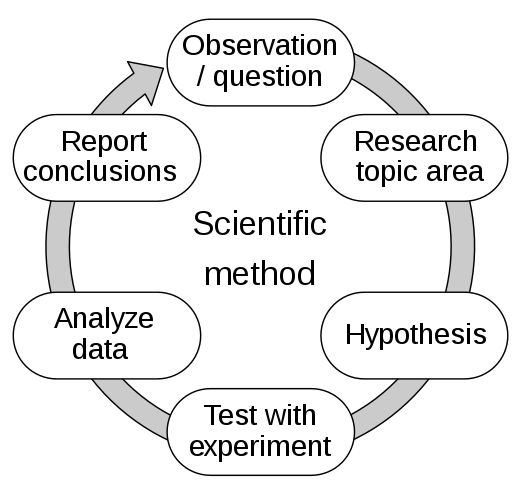
\includegraphics[width=1\linewidth]{imgs/The_Scientific_Method}

\end{floatright50}

A researcher today might begin with an \textbf{observation}--like, I find some tastes delicious and others repulsive-- or, a \textbf{question}-- how can I read a book faster?. Given that cognition has already been studied for well over a hundred years, a next step could be to understand the previous literature, if it exists, on the topic or question. For example, a good place to start would be searching \href{https://scholar.google.com}{Google Scholar} for primary research articles that have asked similar questions.

\textbf{Prior research} can often help you understand the current state of knowledge about a question. For example, if you want to read a book faster, you should read the review article, ``So Much to Read, So Little Time, How Do We Read, and Can Speed Reading Help?.\footnote{\protect\hyperlink{ref-raynerMuchReadLittle2016}{Rayner, K., Schotter, E. R., Masson, M. E., Potter, M. C., \& Treiman, R. (2016). So {Much} to {Read}, {So Little Time How Do We Read}, and {Can Speed Reading Help}? \emph{Psychological Science in the Public Interest}, \emph{17}(1), 4--34. \url{https://doi.org/gdm2ss}}.} This article covers many important previous results in the reading literature that someone should be aware of before they conduct their own research. Unfortunately, it turns out that there is no known simple and easy method to dramatically improve reading speed without also sacrificing comprehension.

Nevertheless, let's imagine a researcher has familiarized themselves with the previous literature, and then they come up with a new \textbf{hypothesis}. For example, maybe reading speed could be improved if fonts for text were redesigned to make visual processing faster. Perhaps similar formatting changes could be made for braille or other reading methods that would influence reading speed. Ideally, hypotheses should have testable implications that can be measured.

Next, the hypothesis is put to a \textbf{test with an experiment}. The purpose of the experiment is to create a controlled situation where aspects of the hypothesis are manipulated to determine whether they influence the measurements. For example, a researcher might create two kinds of fonts, \textbf{some fonts could be presented in bold}, and \emph{other fonts could be presented in italics}. Then, people could volunteer to read words presented in both fonts, and the researcher could measure reading speed.

The experiment generates measurements in the form of data that is collected under different experimental conditions. A next stage in the cycle is to \textbf{analyze the data}, and determine whether the manipulations had any influences. For example, if font type reliably influences reading speed, then the data should show that reading speeds are reliably slow for some fonts, and reliably faster for others.

The research cycle ideally involves a community of peers, so the final stage of a research project could be to \textbf{report conclusions}, or otherwise communicate the results of your research. This is typically done by writing up a research report and submitting it for peer-review to a journal. The peer-review process can help identify areas of improvement that the researcher may address in a revision. If the journal accepts the paper, then it becomes a part of the literature on that subject.

Fact and theory generation are a part of the research cycle. Fact and theory generation is the process of figuring out what facts about cognition are real and in need of explanation, and then coming up with theories that explain the facts. The research cycle can be used to test factual claims and theoretical claims, which can lead researchers to discover new facts and create new theories (i.e., a cyclical process). Last, cognition research is a human activity that is embedded within a socio-historical context. The discoveries of cognitive research can have applications in society (for better and worse), and the potential prospects of these applications can in turn influence the research process by guiding researchers to spend their time on some problems as opposed to others.

\hypertarget{experiments-and-measurements}{%
\subsection{Experiments and measurements}\label{experiments-and-measurements}}

Cognitive research often involves formal experiments and controlled measurements. This textbook assumes you may be unfamiliar some aspects of experimental methods in psychology, and that is OK. We will cover important experimental details when necessary throughout the textbook.

Experiments are used to manipulate an \emph{independent} variable (like type of font) and measure the influence (or lack of influence) on a \emph{dependent} variable (like reading time). If the experiment is properly controlled and free from confounding variables, then experiments showing positive results suggest a causal connection between the manipulation and the measurement. There are an enormous number of experimental procedures, manipulations, and measurements that have been tailor made to answer questions about cognition.

In some research domains the objects of inquiry can be measured directly. For example, geologists can measure rock formations, biologists can inspect cells with a microscope, and neuroscientists can measure action potentials of single neurons. In cognition, the objects of inquiry are often cognitive processes that can not be measured directly. Instead, inferences about cognitive processes are made from indirect measurements.

Consider your ability to form thoughts, and more specifically your ability to generate examples from a category. For example, how many names of mammals can you write down in 5 minutes? Your ability to generate many mammal names is assumed to be driven by cognitive processes involved in language, semantics, categorization, memory, thinking, motor movements, and others; all of which are instantiated in a complex network of physical and physiological processes. As a result, the cognitive processes involved in something as simple as thinking of animal names are complex and not easy to directly measure. Instead, a behavioral measure of task performance is directly observable, and is used to make inferences about the cognitive processes producing the behavior. In this case, example behavioral measures could be the number of animals someone wrote down, how long it took to write each name down, and even patterns like the order and grouping of how the names were written down.

In general, measurements in cognition are taken while a participant is performing a task. Measurements are often behavioral aspects of task performance, but may involve measures of physiological processes like heart rate, or brain processes as well. Common behavioral measurements include accuracy and reaction times to complete actions or portions of a task. Technology like eye-trackers can measure eye-movements during task performance; or systems like the X-box \href{https://en.wikipedia.org/wiki/Kinect}{Kinect} can be used to for body motion sensing. People are often asked to make judgments on various rating scales, and generate or produce information like words or drawings. Common physiological measurements include heart rate, skin-conductance, and pupil-dilation, which sometimes correlates with cognitive activities. Common non-invasive neuro-physiological techniques include \href{https://en.wikipedia.org/wiki/Electroencephalography}{EEG}, \href{https://en.wikipedia.org/wiki/Functional_magnetic_resonance_imaging}{fMRI}, \href{https://en.wikipedia.org/wiki/Magnetoencephalography}{MEG}, and \href{https://en.wikipedia.org/wiki/Positron_emission_tomography}{PET}, for measuring correlated brain activity during task performance.

Finally, measures of cognition are not set in stone, and researchers may find creative ways to gain traction on cognitive phenomena. One of my favorite examples of a clever measurement is from Patrick Rabbitt, who was investigating the skill of typewriting on mechanical typewriters.\footnote{\protect\hyperlink{ref-rabbittDetectionErrorsSkilled1978}{Rabbitt, P. (1978). Detection of errors by skilled typists. \emph{Ergonomics}, \emph{21}(11), 945--958. \url{https://doi.org/bsv6k8}}.} He wondered whether typists might hit keys more softly when they make errors, perhaps because they knew they were making an error, and were trying to stop the keystroke. The clever bit was how to measure response force without creating a special typewriter capable of measuring forces for individual key-presses. Rabbitt had typists type on layers of carbon paper using a mechanical typewriter. With this apparatus harder keystrokes would impress on deeper layers of the carbon paper, while softer keystrokes would only impress faintly on shallower layers. Rabbitt did find evidence that typists pressed keys more softly when they were making some errors. This is an example of a finding or phenomena which we discuss next.

\hypertarget{findings-effects-and-phenomena}{%
\section{Findings, effects, and Phenomena}\label{findings-effects-and-phenomena}}

The research cycle in cognition has produced numerous findings, effects, and phenomena. A \textbf{finding} refers very generally to results from the research cycle. For example, Rabbitt found that typists press keys a little bit more softly for some of the errors that they committed. Another general word for \emph{finding} is observation, and we could say that Rabbitt observed soft responses during error production in his study. I'll reserve the word \textbf{effect} for findings that are the result of an experimental manipulation, especially where the manipulation has an effect on the measurement. Finally, phenomena refers to classes of related findings or effects.

\begin{floatright50}
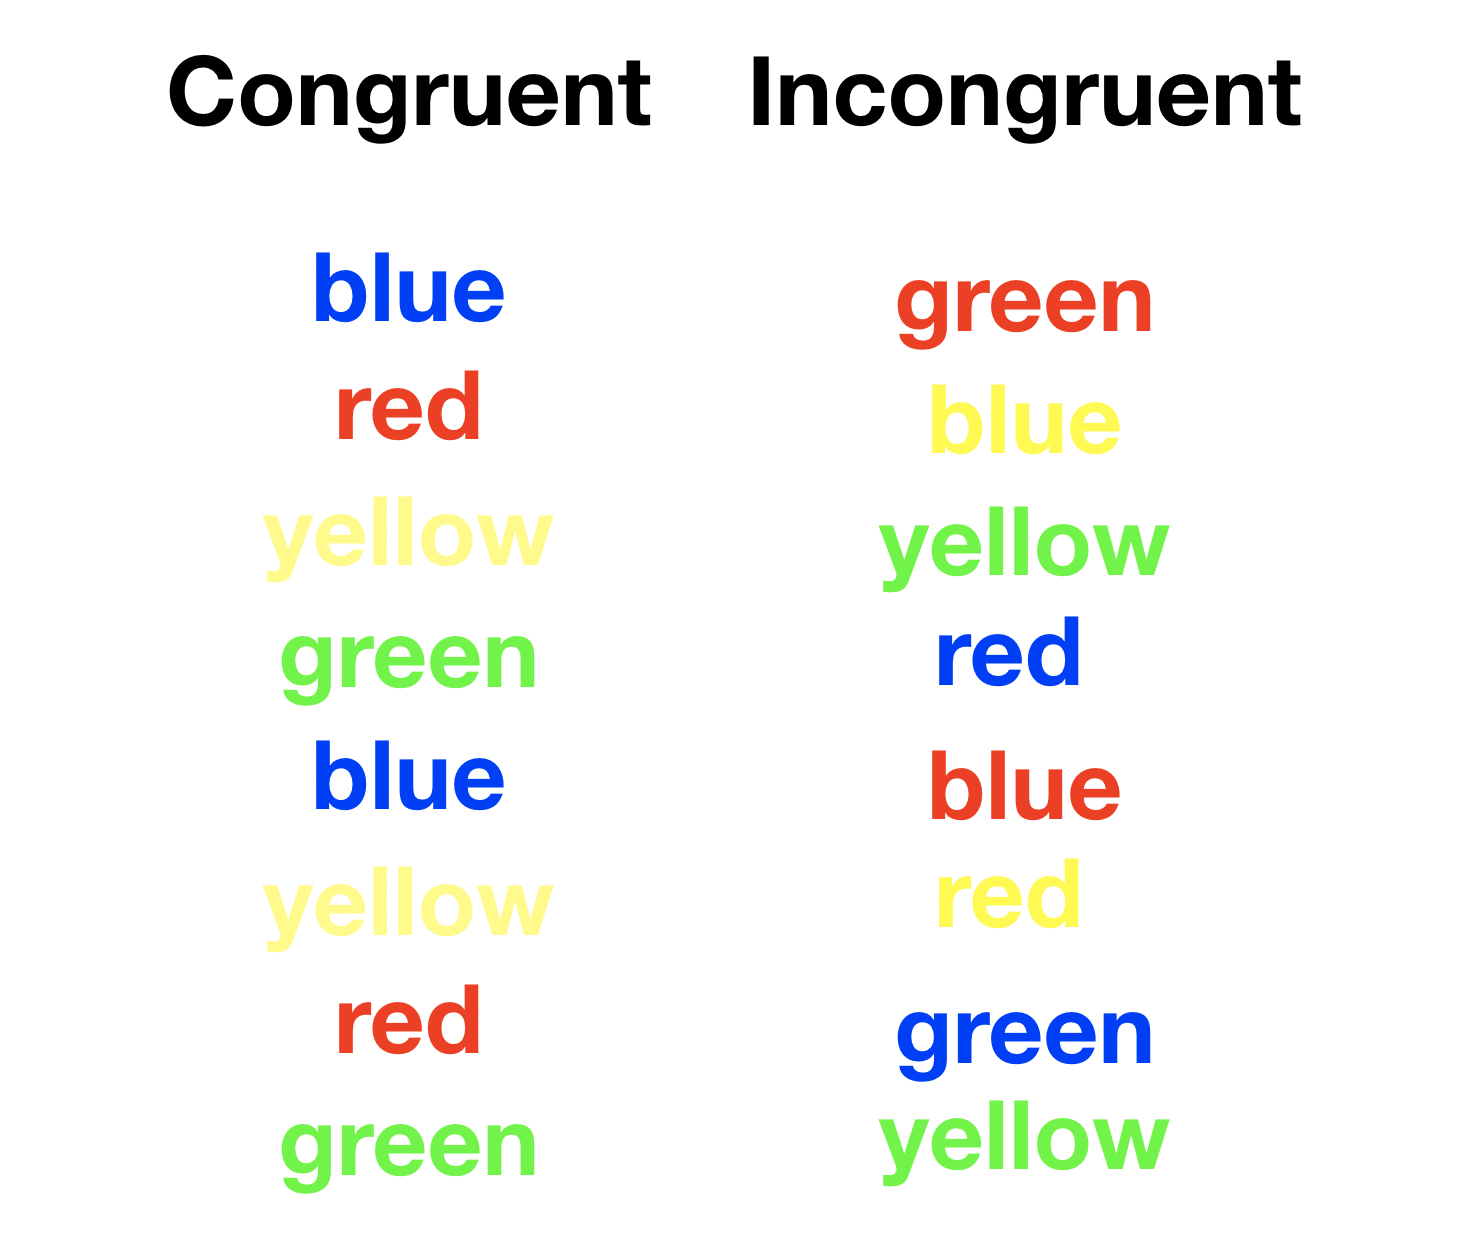
\includegraphics[width=1\linewidth]{imgs/Stroop_stim}

\end{floatright50}

The Stroop effect\footnote{\protect\hyperlink{ref-Stroop1935}{Stroop, J. R. (1935). Studies of interference in serial verbal reactions. \emph{Journal of Experimental Psychology}, \emph{18}(6), 643--662. \url{https://doi.org/b77m95}}.} provides a useful example. In a Stroop task, subjects are shown stimuli like in the example to the right, and asked to name the ink-color of the stimulus on each trial. For congruent stimuli, the ink-color matches the name of the word, like the color blue in the word BLUE. The correct answer for this stimulus is \emph{blue}. For incongruent stimuli, the ink-color does not match the name of the word, like color red in the word GREEN. The correct answer for this stimulus is \emph{red}. The typical finding in this procedure is that participants are faster and more accurate to identify congruent than incongruent stimuli. This difference is termed the Stroop effect \footnote{named after J. R. Stroop who first discovered them}, which refers to the effect of the congruency manipulation on the reaction time or accuracy measure. Stroop effects can be obtained with many different combinations of stimuli that involve manipulations of matching and mismatching target and distractor dimensions, and they have the subject of many investigations for various reasons \footnote{see the chapter on Attention}, and collectively are referred to as Stroop phenomena \footnote{and several other terms, including congruency phenomena, compatibility phenomena, interference phenomena, and cognitive control phenomena}.

There are too many findings in cognition to discuss in a single book. This textbook will aim mostly for breadth to give readers a high level overview of many findings and phenomena. On occasion we will also inspect particular findings and phenomena with additional depth to examine how experiments are used to evaluate process-based explanations of findings and phenomena.

\hypertarget{explanations-theories-and-models}{%
\section{Explanations, Theories, and Models}\label{explanations-theories-and-models}}

Just like we will encounter numerous findings and phenomena across many domains in cognition, we will visit almost as many theories, models and general approaches to explaining those phenomena. There is no single agreed upon format for theories or models, so explanations take a variety of formats, from informal verbal theories to formal mathematical models. Explanations can also be aimed at different levels of analysis, and they are often metaphorical in nature.

One of the problems with explaining how cognition works is that cognitive systems-- like people and animals-- are extremely complex and made up of many interacting physical parts. The complexity makes a reductionist account of cognition very challenging because there are so many parts and pieces of parts to explain. For example, a reductionist theory might attempt to explain a cognitive phenomena like human memory in terms of the operation of physiological substrates in the brain, which would require an explanation of how neuronal processes work at an electrical and biological level, which would require explanations in terms of physics and chemistry and so on. Physiological accounts of cognitive phenomena are one standard for reductive explanation, but there are others as well.

\hypertarget{levels-of-analysis}{%
\subsection{Levels of Analysis}\label{levels-of-analysis}}

Another approach to explanation in cognition invokes the concept of multiple levels of analysis Pylyshyn, Z. W.\footnote{\protect\hyperlink{ref-pylyshynComputationCognitionFoundation1984}{(1984). \emph{Computation and cognition: {Towards} a foundation for cognitive science}. {Cambridge, Ma: MIT Press}}.} For example, vision scientist David Marr described three levels of analysis for the task of explaining visual perception from a computational perspective.

Consider first that vision involves a series of transformations beginning at the moment where light hits the retina. From here, photo-receptors in your eyes convert light into electrical impulses sent through the optic nerve, past the optic chiasm, where they are received by neurons in the lateral geniculate nucleus in the thalamus, which is further connected to primary visual areas at the back of the brain. Somehow the visual processing pathways of the brain turn patterns of light falling on the retina into perceptions. Marr considered this system from a computational perspective involving three levels of analysis \footnote{As a quick sidenote, the computational view of cognition will receive much more elaboration across the textbook}.

Marr's likened visual processing to information processing in a computer system, and suggested that both should be understood in terms of three levels of analysis: computational, representational or algorithmic, implementational or hardware.

\hypertarget{computational-level}{%
\subsubsection{Computational Level}\label{computational-level}}

The computational level refers to the overall goal of a process. For example, what is the computational purpose of an eyeball? At this level, and in the context of the rest of the visual system, the goal of eyeballs could be to transduce light photons into electrical signals for further processing. At the computational level it is possible for the goal to be realizable in multiple ways. For example, smart phones with digital cameras also have a lens system to convert photons into electrical signals. So, if you were to imagine yourself as an alien researcher wondering about eyeballs or digital camera lens, one level of explanation involves understanding the purpose or goal of the system, which in this case would be to capture and convert light for further processing.

\hypertarget{representational-or-algorithmic-level}{%
\subsubsection{Representational or Algorithmic Level}\label{representational-or-algorithmic-level}}

The representational or algorithmic level refers to the steps taken to achieve the computational goal. A The cooking metaphor developed later in the chapter is useful here. For example, you might have the goal (computational level) of making chocolate chip cookies. The ingredients and steps in the recipe you use to make chocolate chip cookies is a good example of the representational or algorithmic level of analysis. The representations refer to the inputs and outputs of the process, such as the raw ingredient inputs, and the cookie outputs. The algorithm refers to the step-by-step instructions for transforming the inputs to the output. A good recipe for making chocolate chips contains a reasonably precise high-level description of the ingredient list (representations), and the combination and cooking instructions (algorithm) to create tasty cookies.

To return to the domain of vision, photons are the representational inputs of eyeballs and digital cameras. The algorithm in either system refers to the steps, or way in which, the inputs are transformed into the electrical signals as outputs.

\hypertarget{hardware-implementation}{%
\subsubsection{Hardware implementation}\label{hardware-implementation}}

The hardware implementation level refers to how the representations and algorithm used to accomplish a computational goal are instantiated in a physical system. For example, what specific physical elements and processes enable an eyeball to transduce light into electrical signals? Similarly, what specific physical elements and processes enable a digital camera to capture images and store them in computer memory?

\hypertarget{summary}{%
\subsubsection{Summary}\label{summary}}

Using Marr's levels as a guide, this textbook will mostly focus on computational and algorithmic levels, rather than on the hardware implementation level. If you are a student at Brooklyn College taking this introductory course in cognitive psychology, you will find more elaboration on brain mechanisms supporting cognition in other courses such as Mind, Brain and Behavior.

\hypertarget{metaphorical-models}{%
\subsection{Metaphorical Models}\label{metaphorical-models}}

Metaphorical models are also common strategies for explanation in cognition. Metaphorical models refer to the process of mapping a simple model system as a metaphor for describing and understanding another more complicated system. For example, horse-racing has been used as a model for explaining the Stroop effect. The basic idea is that word and color (or target and distractor) information compete for identification, just like horses running down a track compete to get across a finish line. The metaphor does not assume that people have horses or a race-track in their brains. Instead, the metaphor provides terms and functional relationships that can provide well-fitting descriptions of Stroop phenomena, and even make predictions about what might happen to the effect under different experimental manipulations. Metaphorical models can be informal and verbal, like how I have just loosely described stimulus identification in terms of a horse-race; and, they can be more formal and mathematical. We devote a whole chapter to computational theories to provide some more detailed examples of formal theorizing in cognition.

\hypertarget{applications}{%
\section{Applications}\label{applications}}

To simplify some of the preceding discussion up to this point, the research cycle in cognition produces theory and phenomena, and both theory and phenomena can lead to applications. For example, theory about how people learn skills could be used to modify training curriculum and enhance the skill-learning process. Even seemingly strange laboratory phenomena like the Stroop effect can have inventive applications. For example, Stroop effects have been used to detect whether or not a person may be a spy. For example, during world war II, a German spy may claim not to speak German, but a Stroop test involving German words could reveal large interference effects, indicating they do speak the language.

Throughout the textbook I will aim to point out similar applications that have already sprouted from various domains in cognition. And, time permitting, I am planning to include a chapter on cognitive technologies to highlight applications from the past and present, as well as expected future directions. Daily life is increasingly mediated by interactions with smart technologies, and applications from cognition to technology are occurring at a rapid pace. For example, when I was an undergraduate in the early 2000s we didn't have smart phones, and the problem of recognizing faces in photographs was not an easy problem for computers at-the-time to solve. However, today most phones have face-recognition built-in, and deep-neural networks can make convincing fake videos of real people--and, the cognitive sciences have facilitated both of those technological developments and more.

\hypertarget{implications}{%
\section{Implications}\label{implications}}

Cognitive research has been developing and ongoing for well over a century. In that time, many theories, findings, and applications have been produced. At the same time, research into cognitive abilities has not always had uniformly positive implications for society, and there are examples where research applications were severely destructive for some groups of people. I think issues of equality and justice are important when discussing cognitive research and its applications, so I will also touch on these topics. One way I will do this is by occasionally discussing historical context around the research and researchers that we discuss. To take one example, we will examine how research on mental imagery ability and the early development of intelligence testing were influenced by the widespread eugenics movement of the time. This era of psychology made a deep impression on subsequent cognitive research, and raises important questions about how psychological can and should be applied in society.

\hypertarget{questions-to-keep-in-mind-as-you-learn-about-cognition}{%
\subsection{Questions to keep in mind as you learn about cognition}\label{questions-to-keep-in-mind-as-you-learn-about-cognition}}

What are the goals of the cognitive sciences and research in cognitive psychology? Who has been involved in setting those goals? Are the goals useful? What kind of questions about cognition have already been asked by researchers? What were the scientific as well as social-historical reasons for why those researchers asked those questions? What answers were found, and how were they informative or not informative about how cognition works? How do the measurements and tools that researchers use to ask questions influence the kind of picture they build about how cognition works? What kinds of questions about cognition are not being asked that should be asked? Why are they not being asked? What benefits to society have been produced by the cognitive sciences? Have the benefits been spread equitably across different groups of people? What costs to society have been produced by the cognitive sciences? How are the costs shared by society? Are there injustices resulting from cognitive science research? Have they been adequately addressed? How should society decide whether or not to proceed with different kinds of research?

\hypertarget{the-cooking-of-science-a-recipe-metaphor}{%
\section{The cooking of science: A recipe metaphor}\label{the-cooking-of-science-a-recipe-metaphor}}

This last section provides a cooking or recipe metaphor for the research cycle in cognition. The recipe metaphor is intended to orient you toward major features of theories, explanations, and how they are tested across the research cycle \footnote{This section starts to get into larger issues in philosophy and the philosophy science, which are beyond the scope of this book. I will attempt to make connections to these domains as much as possible throughout}. A recipe is a set of instructions for how to do something like cook a dish or put together furniture from IKEA. Recipes can take different formats (e.g., written recipes in a cookbook, cartoon's in an IKEA manual, or even do-it-yourself YouTube videos). Recipes can be more or less specific. Some cookbooks break down every single step in making a dish, others give general directions (e.g., cook it until done). Recipes have the goal of communicating instructions about how to do something. And, it is possible to evaluate recipes to see whether or not they accomplish the goal. For example, if a recipe works, and I know how to follow instructions, then I should be able to follow the recipe and make the thing that the recipe produces. Sometimes a recipe turns out (it does what it says it does), and sometimes it doesn't. When a recipe doesn't work it could be that the recipe instructions had mistakes, were confusing, or were not followed properly (problems with execution). It's also possible that a recipe is totally flawed and does not do what it claims to do.

Everyday recipes are explanations about how something works, and the properties of recipes are very much like the properties of theories in cognition. I would say that as a cognitive scientist, I am interested in the ``recipes of cognition'', and I find explanations about cognitive abilities very satisfying when they have all of the properties of a really good recipe. For me, a really good recipe 1) does what it says it does, and 2) strikes a delicate balance between describing all of the necessary steps in intricate detail, and elegantly describing the most important steps, connections between steps, and general principles that provide insight into the steps. In other words, a great recipe achieves a ``productive level of vagueness'' \footnote{I attribute this phrase to Lee Brooks, who often suggested that theories in cognition need to find a productive level of vagueness, that are specific enough to be meaningful, general enough to be interesting, and workable enough to create insights}.

\hypertarget{oven-fries-my-favorite-recipe}{%
\subsection{Oven Fries: My favorite recipe}\label{oven-fries-my-favorite-recipe}}

Let's take a break from asking how a cognitive ability works, and ask how tasty, crispy, super-delicious oven-fries work. For a long time I didn't really like oven-fries, I much preferred french fries. But, my whole life changed when I found my favorite recipe of all-time, the ``Oven Fries'' recipe from America's Test kitchen.\footnote{\protect\hyperlink{ref-illustratedNewBestRecipe2004}{Illustrated, C. (Ed.). (2004). \emph{The {New Best Recipe}}. {America's Test Kitchen}}.}

America's Test Kitchen writes very compelling recipes. I had tried making fries in the oven before. They always came out terrible. They always stuck to the pan, weren't crispy or delicious. But, I knew it must be possible to make yummy fries in the oven because I had them before with friends or at restaurants. I needed to know the magic behind good oven fries, and everything I needed to know was in the America's Test Kitchen recipe.

America's test kitchen uses the same basic research cycle to improve their recipes as cognitive scientists use to study cognition. This involves experimentally manipulating parts of the recipe to see what matters in making a good dish \footnote{there is also a healthy dose of using general principles about cooking food to inform the choices they make about what parts of the recipe to manipulate}. For example, the cookbook I have has both a great recipe for oven fries, and a short research report on all of the experiments that went into figuring out the recipe. They baked potatoes at different temperatures, put the pans on different racks in the oven, boiled the potatoes first, left skin on or skin off, tested different kinds of oil, and so on. They manipulated each of these components, made different batches of fries, and then had people taste the results each time. As they tried different combinations, they kept instructions that seemed to work well, and slowly developed a recipe that produced really tasty fries that were given really high ratings by the tasters. One fantastic insight was to salt the pan before putting the potato wedges on them, which helps reduce sticking to the pan later on. Anyway, I love this recipe for two reasons. First, it works and delivers great tasting oven fries. Second, it is insightful about what the recipe is doing, and helped me appreciate principles of cooking that I have applied to other dishes.

\hypertarget{cooking-competitions-and-the-best-recipe}{%
\subsection{Cooking competitions and the best recipe}\label{cooking-competitions-and-the-best-recipe}}

The last piece of the recipe metaphor I'm building here comes from the TV show Top Chef, where chef contestants compete with each other to become the Top Chef. One of the challenges is about writing a good recipe. Each of the contestants makes up a dish and writes down a recipe for how to make the dish. The big twist is that they don't get to cook the recipe. Instead, other people have to try and follow the recipe to make the dish, and the chef's are judged on how well those dishes turn out. What really matters for this challenge is that the recipe provides a clear explanation of how the dish works. Let's use a similar kind of situation as a metaphor to examine properties and qualities of explanations in cognitive research.

In the metaphor, a recipe is like a theory about how something works. A recipe contains elements, like individual steps to follow to produce an outcome. Similarly, a theory contains components, like individual assumptions and propositions that work together to produce an explanation. So, if we are comfortable with recipes and theories being very similar, how can they be evaluated for their explanatory value? Are some recipes/theories better or worse? Are some recipes/theories true or false? Answering these questions involves an iterative research cycle where recipes/theories are put to the test and refined over time. Let's examine this with an imaginary scenario.

Imagine you are a chef-scientist and chief detective, and you have been asked to solve a food mystery. You arrive at a dinner table, and your host brings in a big silver plate with a big silver dome. The cover is removed to reveal your favorite dish. You eat it, and it is the best version of this dish you have ever tasted. The host challenges you to explain how the dish was made. Your task is to make a recipe and show that you can use it to recreate the dish.

Fortunately, you do not have to start entirely from scratch. There is a well-stocked kitchen with all of the ingredients and equipment that you might need, and even many cookbooks that might contain the recipe you are looking for. You are allowed to run experiments in the kitchen to help you figure out how to make the recipe. What do you do? How do you figure out the recipe? I will offer some opinions on things that could happen in this scenario and relate them to parts of the research cycle in cognition.

First of all, you would probably use some \emph{background knowledge} to help guide you toward a solution. For example, if you knew some of the ingredients in your dish, you would probably use those in your experiments. If you knew the name of the dish, then you might search the cookbooks for different versions of recipes for the dish, and try each of those out to see if one of them made the dish. People have unique background knowledge, and in the context of research bring different initial working assumptions to the research cycle. If you didn't know oven fries used potatoes, you might have test out different vegetables until you found the right ingredients.

The goal is to create a recipe that recreates the dish, and there are many available recipes in the cookbooks. Similarly, a goal in cognition is to explain cognitive abilities with theories, and there many available theories in the literature. One way to test the recipes is to try them out, and examine the final product to see if it is the same as the dish you are trying to recreate. Let's consider going through the motions of testing many different recipes.

\hypertarget{recipe-quality}{%
\subsection{Recipe Quality}\label{recipe-quality}}

Some recipes will work pretty well, and if you try them out you might produce dishes that are close to the dish you are trying to recreate. For example, you could easily find three longer recipes for oven fries that all work well. Similarly, in cognition it is possible to find multiple working theories of a cognitive ability that all do an OK job of explanation.

Some recipes might be extremely vague. For example, Oven Fries: Get some potatoes, and bake them on a pan in the oven until they are perfect. This is a like a ``theory'' that is really just a couple basic claims, and not much else.

Some recipes will be broken or nonsense. Here is a nonsense recipe for oven fries: peel bananas, put them in a blender, pour them over coffee, stick the coffee in the microwave, and then eat a raw potato. This has the appearance of a recipe because it lists ingredients and steps, but upon closer inspection, it should be clear that following the steps will not lead to the creation of oven fries. In the domain of cooking, broken recipes fail to produce the dish they claim to make. In cognition, theories can fail to produce explanations they claim to make. Just like a nonsense recipe, a theory might not contain enough coherent assumptions and steps to produce a desired explanation.

I described good, bad, and ugly recipes that range in quality for producing a dish. If we are still trying to recreate create the best dish, a next task is to refine and improve the recipe using a research cycle. This will involve testing assumptions in the recipes to learn which steps and ingredients are necessary, proposing and testing new steps in the recipe that weren't there before, and possibly even completely rewriting the recipe if you found a more compelling way to make the dish.

\hypertarget{testing-recipes}{%
\subsection{Testing Recipes}\label{testing-recipes}}

I'll finish off this metaphor by discussing two kinds of tests that are relevant when we go back to examining theories in cognition. \textbf{Logical tests} are useful for examining the internal structure of a theory to determine whether it is logically possible that the theory can do what it claims to do. This is like evaluating whether or not a recipe can make the dish it claims to make. Logical tests can often be conducted just by reasoning through the theory (or reading through the recipe). For example, it is clear by reading the nonsense recipe from above that it will not do what it claims to do. When you are visited with theoretical claims about cognitive abilities, it should be possible to read through the theory like a recipe and clearly appreciate how the claims about cognition work.

\textbf{Empirical Tests} are useful for examining components of a theory, and they typically involve experiments to measure phenomena that are associated with claims or assumptions from a theory. For example, in my favorite recipe for oven fries, one of the tips is to salt the pan that you put your potato slices on\ldots this is supposed to help reduce the fries sticking to the pan. Let's think of ``Salting the pan'' as one critical part of the ``theory of oven fries''. How critical is this assumption? Is it necessary for making oven fries? Does salting the pan actually reduce stickiness? These questions can be answered with an experiment to address the question.

The experiment will involve making different batches of oven fries, some where the pan is salted, and others where it is not, and then measuring how much the fries stick to the pan. More formally, this experiment will involve an \textbf{independent variable} that is manipulated by me, the experimenter--the experimental manipulation is salting the pan. The manipulation will have at least two levels or conditions, so that the outcomes can be compared between them. In the \textbf{control} condition I won't add salt to the pan. In the \textbf{experimental} conditions, I will add salt to the pan. I could even try different amounts of salt if I wanted. To run the experiment I would try to follow the oven fries recipe exactly the same way for every batch of fries of that I make, with the only difference being whether or not I salted the pan. I will even make sure that each pan has the same number of potato wedges on it. Then, for each batch I will need to measure the stickiness of the fries somehow. This measurement is called the \textbf{dependent variable}, because it is supposed to depend (or be influenced by the experimental manipulation). How about this, after baking, I will turn the pan upside down. All of the fries that fall off didn't stick. Then I will count all of the fries that did stick.

I can use my observations in the form of counts to evaluate my \textbf{empirical question}, which is a kind of question that can be answered by observing what happens under controlled conditions. My question was whether salting a pan actually reduces the number of fries stuck on the pan. I can count how many fries stuck to pans that were salted, and how many fries stuck to pans that were not salted. And, then I can compare the numbers. If salting the pan doesn't really change fry stickiness, then I would expect roughly the same number of fries on salted and unsalted pans. If salting the pan reduces fry stickiness, then there should be fewer fries stuck on the salted pan than the unsalted pan. Maybe salting the pan actually does the opposite of what the theory claimed, and then there would be more fries stuck on the salted pan than the unsalted pan. If everyone in the world tried making oven fries using different kinds of potatoes, and different ovens, and different pans, and everyone found pretty much the same results, we could become fairly confident in decidedly answering this one question. Or, the results could be a little bit messy, maybe some salt works sometimes for some potatoes on some pans in some ovens, but not others\ldots the empirical answer could be ``maybe, it depends''.

Because I am having fun with this recipe metaphor for science, I'm going to keep going. Let's imagine our experiment shows consistent evidence that salting the pan does reduce the number of fries stuck to the pan. By consistent evidence I mean that I ran the whole experiment a bunch of times and kept getting the same results, so I stopped running the experiment because I felt confident that the result can be trusted. For example, if someone else came over to my kitchen and did my experiment under the same conditions, they would also find that salting the pan reduces how many fries are stuck the pan. Reproducibility of results is also important in cognition, and sometimes it is a concern because there are numerous examples of reported experiments whose results have not been consistently reproducible \footnote{we will discuss some examples throughout the textbook and elaborate on issues of reproducibility later on}.

\hypertarget{making-inferences-about-recipes}{%
\subsection{Making inferences about recipes}\label{making-inferences-about-recipes}}

But, for sake of argument, we will assume the salting the pan trick is reproducible. Great. Now what. Let's not forget some of the larger issues at hand. Sometimes we can sucked into a long and detailed story about a specific thing-- like salting a pan of oven fries--and lose track of how this little story fits into the bigger issues. I set up the salting-the-pan experiment because it was a way to put a component of the oven fry recipe to the test. What have we learned through the process of putting this one component of the recipe to an empirical test? How are results from empirical tests used in the process of improving our explanations of the things we are testing? In my opinion, there is a long and artful dance that occurs between explanations (in the form of theory) and empirical results (in the form of data), that eventually lead them to embrace one another.

In our thought experiment, the original question of interest was ``how do the best oven fries work?''. What inferences about the overall recipe can we make based on the empirical test of one of its assumptions? In terms of making inferences about theoretical assumptions from data, the available inferences will be limited by how the assumptions fits in the theory, and what the pattern of data says about the assumption. Is salting-the-pan a necessary assumption for really great oven fries? That invites another empirical question that we didn't ask. Are the fries from the unsalted pans still really good? If so, then salting the pans might not be a necessary step in the recipe (even if it does reduce stickiness). What are the necessary steps from the recipe? We could spend time creating individual experiments to test whether each step and ingredient, or specific combinations of the steps and ingredients are all necessary or not necessary to make great fries. When you consider the number of steps, ingredients, and slightly different variations, and number of ways that all of these things can be combined, there are a never-ending number of experiments that could be run to empirically test assumptions of the recipe. I'm exhausted just thinking about it. If we forced ourselves to test all of the combinations we would never leave the kitchen, or do anything else.

Asking empirical questions to settle one issue can easily open new questions about other issues that may or may not be of interest. For example, demonstrating empirically that salting the pan does reduce the number of fries stuck to it, raises new questions about how stickiness works. How does salt change the stickiness of pans? The evidence that salt does change stickiness becomes a phenomena in and of itself that requires explanation, and we would need to drop into the territory of chemistry and physics to examine those issues.

\hypertarget{dessert}{%
\subsection{Dessert}\label{dessert}}

I should bring this metaphor to a close, but here are some parting thoughts. The things that you might want out of a cooking recipe are not too different from what you might want out a theory in cognition. And, you should feel empowered to evaluate what you learn about cognition from this point of view. It is OK to be unsatisfied with a recipe for many reasons, it might be unclear, it might be complicated, it might not work very well, it might have extra unnecessary stuff; it might look pretty good until it tells you use apply some magic sauce that was never explained. Same goes for explanations of cognition, where you might be unsatisfied for similar reasons.

It is also OK to like different recipes for many reasons. Some recipes are inspiring to read and get you excited, some recipes give super-specific instructions for doing one thing really well, some recipes are surprising and make you wonder what the food would taste like, and some recipes are very insightful and show you techniques that can be used over and over again for other recipes. Same goes for explanations of cognition, where there can be different reasons to appreciate the value of a theory, even if it isn't perfect.

Last, consider the concept of truth in the metaphor between recipes and theories. In the domain of cooking and recipes is there such a thing as true recipes? Is there one true oven fries recipe? I don't think so. There are lots of oven fries recipes. They all make oven fries. Some of them make oven fries that I like more than others. Also, there is an entire world of other recipes and it is very exciting to explore all of the tasty ways that different people and cultures prepare food. What about theories in cognition? Is there one true theory of cognition? If there is, I haven't heard about it. Instead, like recipes there are lots of different theories about cognition, and it is OK to appreciate that variety as we learn about how different researchers have prepared their explanations of different cognitive abilities.

\hypertarget{mental-imagery}{%
\chapter{Mental Imagery}\label{mental-imagery}}

\begin{tabular}{r|l|l}
\hline
Word Count & Reading Time & Last Compiled\\
\hline
8002 & 40 minutes & 2021-09-21 19:59:30 GMT\\
\hline
\end{tabular}

\hypertarget{chapter-overview-1}{%
\section{Chapter Overview}\label{chapter-overview-1}}

This chapter discusses historical and current research on mental imagery. It begins with a review of Sir Francis Galton's early work showing evidence of individual differences in mental imagery. We then turn to more recent work describing extreme differences in mental imagery in terms of aphantasia (lack of mental imagery) and hyperphantasia (very vivid mental imagery). The chapter ends with mental imagery as a possible explanatory process in the domain of memory and mental scanning.

\hypertarget{what-is-mental-imagery}{%
\section{What is mental imagery?}\label{what-is-mental-imagery}}

Close your eyes, and think about what you can see or hear in your ``mind's eye'' or ``mind's ear''. Some people report being able to see life-like images that are extremely clear and vivid, almost as if there is no difference between what they can imagine seeing and what they can see when they are looking at something when their eyes are open. Some people report seeing less vivid mental imagery that is more spatial in nature. For example, they could close their eyes and imagine their kitchen; but they wouldn't ``see'' their kitchen as it appears when they are looking at it for real; but, they would nevertheless have some spatial sense about the shape of the kitchen, and where things are stored in the kitchen. Other people report having very little to no mental imagery.

For fun, I'll tell you what I see when I close my eyes. My eyelids, and not much else\ldots{} it's pretty dark when I close my eyes. At the same, I can imagine my kitchen pretty easily, although, I wouldn't say that I ``see'' it very clearly, I ``see'' it more spatially. However, sometimes I do ``see'' images that are more visual, that look like things I see when I have my eyes open. Also, I've had lots of dreams that seemed very visually vivid and real, just like visual experiences appear to me in waking life. So, according to me, my mental imagery is all of the above, and can include imagery about other kinds of senses, like sounds, taste, touch, and smells.

Let's assume for the moment that mental imagery is a real cognitive ability, and that different people experience mental imagery in different ways. How does mental imagery work? What kind of explanation would we be looking for to answer this question? What steps could we take to start answering this question? How have prior researchers tackled these questions, and what have we learned about mental imagery? How has society been influenced by research into mental imagery and vice versa?

\hypertarget{generating-facts-about-mental-imagery}{%
\section{Generating facts about mental imagery}\label{generating-facts-about-mental-imagery}}

In general, before progress can be made on all of those questions, a first step is to collect information about the features or facts about a phenomena like mental imagery. If we have no facts, there wouldn't be much to explain. So, how do we get facts that we can trust, and collectively agree upon, about a subjective phenomena like mental imagery? My assessment is that the literature has produced many kinds of imperfect measurements that are relevant to the task of establishing facts about mental imagery. Still, a healthy amount of skepticism is required for evaluating what the findings mean. Let's start with perhaps the most obvious way of knowing about mental imagery. Ask yourself what it is like to you, and ask other people what it is like to them.

\hypertarget{methods-of-introspection-and-subjective-report}{%
\subsection{Methods of Introspection and Subjective report}\label{methods-of-introspection-and-subjective-report}}

Mental imagery is all about the subjective experience of being in your own mind. So, by this definition, there is only one person who really knows what it is like to be you, and you are that person. So, if you want to get the facts about your own mental imagery, is it possible for you to do that?

One imperfect solution is called the method of introspection, which means to self-reflect on your experience of your own cognition. Introspection has been, and still is, employed as a tool by many psychologists. For example, early German psychologist \href{https://en.wikipedia.org/wiki/Wilhelm_Wundt}{Wilhem Wundt} (1832-1920) and American psychologist \href{https://en.wikipedia.org/wiki/Edward_B._Titchener}{Edward Titchener} (1867-1927) advocated the use of introspection as a technique to generate knowledge about the mind. The related method of subjective report involves asking other people to introspect and then report on aspects of their own psychology. Subjective report methods are very common today in the form of questionnaires that ask people to make subjective judgments about their own psychology. Before considering the limitations of introspection and subjective report, let's see an example from mental imagery research.

\hypertarget{galtons-statistics-of-mental-imagery}{%
\subsection{Galton's Statistics of mental imagery}\label{galtons-statistics-of-mental-imagery}}

\begin{floatrightbox25}
\textbf{Sir Francis Galton}

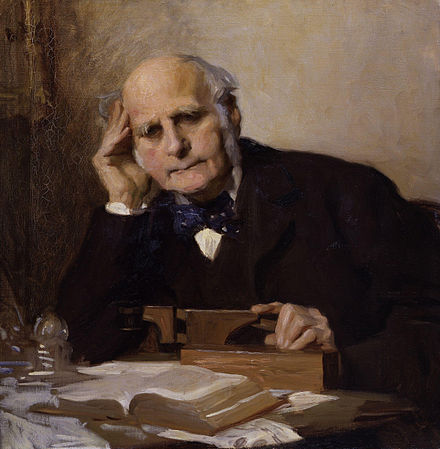
\includegraphics[width=1\linewidth]{imgs/Francis_Galton}

\end{floatrightbox25}

One of the first attempts at studying mental imagery was by Sir Francis Galton.\footnote{\protect\hyperlink{ref-galtonStatisticsMentalImagery1880}{Galton, F. (1880). Statistics of {Mental Imagery}. \emph{Mind}, \emph{5}, 301--318. \url{https://doi.org/gg5vkv}}.} In his paper on ``Statistics of mental Imagery'', Galton set out to ``to define the different degrees of vividness with which different persons have the faculty of recalling familiar scenes under the form of mental pictures, and the peculiarities of the mental visions of different persons.'' How did Galton go about doing this?

\hypertarget{galtons-method-of-subjective-report}{%
\subsubsection{Galton's Method of Subjective Report}\label{galtons-method-of-subjective-report}}

Galton came up with the ``Breakfast table task'', which is a series of structured questions about mental imagery, and then asked 100 people to answer his questions. The basic set of questions is reprinted below:

``Before addressing yourself to any of the Questions on the opposite page, think of some definite object -- suppose it is your breakfast-table as you sat down to it this morning -- and consider carefully the picture that rises before your mind's eye. {[}p.~302{]}

\begin{enumerate}
\def\labelenumi{\arabic{enumi}.}
\tightlist
\item
  Illumination. -- Is the image dim or fairly clear? Is its brightness comparable to that of the actual scene ?
\item
  Definition. -- Are all the objects pretty well defined at the same time, or is the place of sharpest definition at any one moment more contracted than it is in a real scene?
\item
  Colouring. -- Are the colours of the china, of the toast, bread-crust, mustard, meat, parsley, or whatever may have been on the table, quite distinct and natural?''
\end{enumerate}

\hypertarget{galtons-results}{%
\subsubsection{Galton's results}\label{galtons-results}}

Then, Galton recorded the answers that people gave and tried to make sense of them. Here are some of the answers from ``100 men, at least half of whom are distinguished in science or in other fields of intellectual work.'' (reprinted from his original manuscript):

\emph{Cases where the faculty is very high.}

\begin{enumerate}
\def\labelenumi{\arabic{enumi}.}
\item
  Brilliant, distinct, never blotchy.
\item
  Quite comparable to the real object. I feel as though I was dazzled, e.g., when recalling the sun to my mental vision.
\item
  In some instances quite as bright as an actual scene.
\end{enumerate}

\emph{Cases where the faculty is mediocre.}

\begin{enumerate}
\def\labelenumi{\arabic{enumi}.}
\setcounter{enumi}{45}
\item
  Fairly clear and not incomparable in illumination with that of the real scene, especially when I first catch it. Apt to become fainter when more particularly attended to.
\item
  Fairly clear, not quite comparable to that of the actual scene. Some objects are more sharply defined than others, the more familiar objects coming more distinctly in my mind.
\item
  Fairly clear as a general image; details rather misty.
\end{enumerate}

\emph{Cases where the faculty is at the lowest.}

\begin{enumerate}
\def\labelenumi{\arabic{enumi}.}
\setcounter{enumi}{88}
\item
  Dim and indistinct, yet I can give an account of this morning's breakfast table; -- split herrings, broiled chickens, bacon, rolls, rather light coloured marmalade, faint green plates with stiff pink flowers, the girls' dresses, \&c., \&c.~I can also tell where all the dishes were, and where the people sat (I was on a visit). But my imagination is seldom pictorial except between sleeping and waking, when I sometimes see rather vivid forms.
\item
  I am very rarely able to recall any object whatever with any sort of distinctness. Very occasionally an object or image will recall itself, but even then it is more like a generalised image than an individual image. I seem to be almost destitute of visualising power, as under control.
\item
  My powers are zero. To my consciousness there is almost no association of memory with objective visual impressions. I recollect the breakfast table, but do not see it.
\end{enumerate}

\hypertarget{galtons-conclusion}{%
\subsubsection{Galton's conclusion}\label{galtons-conclusion}}

First consider what Galton could have found, and what he might have concluded instead. If you, the reader, have vivid mental imagery, then you might have expected that everyone else does too. In this case, Galton could have found his respondents giving similar descriptions of their imagery. Everybody might have said that they have very strong and vivid visualizing powers. But, it turns out, this is not what people said. Instead, Galton's major conclusion and potential discovery was evidence for a wide variety of individual differences in mental imagery. Some people reported having very strong powers of mental visualization, some people reported having medium abilities, and other people reported having no abilities to visualize anything in their mind's eye at all.

If we are attempting to explain a cognitive ability like mental imagery, and Galton's results provide facts that we can trust, then the task of explaining mental imagery just got a little bit harder. For example, not only do we have to explain how people could visualize a picture in their minds eye, we also have to explain the facts that some people may do this differently, and some people may not be able to do it at all. This is a good example of the increasing complexity that comes along with the research process of gathering facts about a phenomena: asking questions uncovers more facts that raise more questions and require even more explanation.

\hypertarget{limitations-with-galtons-method}{%
\subsubsection{Limitations with Galton's method}\label{limitations-with-galtons-method}}

Galton argued that his methods were useful and appropriate to the task of measuring people's mental imagery abilities, but these introspection and subjective report also have many shortcomings that could easily invalidate all of the results. For example, what if everybody that Galton talked to lied about their mental imagery? In this case, none of Galton's results would be meaningful with respect to understanding mental imagery. Similarly, how accurate are people at describing their own mental imagery? If people are not very accurate, then their descriptions will not be very meaningful for describing their actual experiences. Or, what if people are having the same kinds of subjective mental imagery experiences, but they just use different words to describe the same kinds of experiences. And, of course, maybe everybody was telling the truth and there really are big differences in mental imagery across people.

One big issue here for establishing facts about mental imagery, is that the internal experience of mental imagery is not easy for other people to observe directly. In other domains of inquiry, direct observation can help people quickly establish a set of agreed upon facts. For example, a group of geologists can all look and point at a rock formation, and agree that the rock formation is there, and then proceed to further inspect and measure the rock formation to gather more directly observable facts about it. Galton's method of subjective report does have some directly observable measurements, such as the words that people said about their mental imagery; but, people's verbal statements are at best an indirect attempt to communicate an experience, and do not provide an objective lens for other observers to directly view the experience itself.

If it is not possible to establish objective facts about something subjective like mental imagery, how could we possibly hope to explain those facts given that we may not be able to agree on what the facts are in the first place!?! This is undoubtedly a challenge, and there many tools and methods that cognitive researchers have developed since Galton to help make progress on the issues. One common requirement for establishing facts is to show that they are reproducible. Let's take a look a the reproducibility of some of Galton's claims and findings

\hypertarget{reproducing-galtons-mental-imagery-work}{%
\subsection{Reproducing Galton's mental imagery work}\label{reproducing-galtons-mental-imagery-work}}

Galton conducted his work in the United Kingdom throughout the last half of the 1800s, and like some of his other ideas (that we will discuss in the next chapter), they tended to spread among psychologists in other countries. At the turn of the century, American psychologists were busy using Galton's methods and publishing on the mental imagery abilities of college students. For example, in 1896, Armstrong\footnote{\protect\hyperlink{ref-armstrongjrImageryAmericanStudents1894}{Armstrong Jr, A. C. (1894). The imagery of {American} students. \emph{Psychological Review}, \emph{1}(5), 496. \url{https://doi.org/dkhdx2}}.} used the same ``Breakfast Table'' questions as Galton did, but gave them to students at Wesleyan University (a male college). The general pattern of results was similar to what Galton found. The students reported a wide range of mental imagery abilities, including a small proportion of students who were classified as having little to no visual imagery.

However, in 1902, French\footnote{\protect\hyperlink{ref-frenchMentalImageryStudents1902}{French, F. C. (1902). Mental imagery of students: {A} summary of the replies given to {Titchener}'s questionary by 118 juniors in {Vassar} college. \emph{Psychological Review}, \emph{9}(1), 40. \url{https://doi.org/cqj438}}.} asked students at Vassar college (a female college) about their mental imagery abilities with a longer mental imagery questionnaire (by Titchener),\footnote{\protect\hyperlink{ref-titchenerExperimentalPsychologyManual1905}{Titchener, E. B. (1905). \emph{Experimental psychology: {A} manual of laboratory practice} (Vol. 2). {Johnson Reprint Company}}.} that was intended to improve on Galton's original questions. The results were mostly consistent with prior results, and the Vassar students reported a wide range of different mental imagery abilities. But, one finding was not reproduced. All of the 118 students reported at least some mental imagery abilities, and none of them reported that they had zero mental imagery abilities. This could mean all of the students happened to have mental imagery abilities, or it could call into question the claims that some people do not have mental imagery. One possibility is that the results depend on the questionnaire. Galton had 10 questions about mental imagery, Titchener had almost 90 questions that covered imagery for more senses, and potentially gave students more opportunities to claim that they had at least some mental imagery. Perhaps, Galton and Armstrong would have found all of their participants reporting at least a little bit of mental imagery if they had used the newer questionnaire by Titchener.

\hypertarget{aphantasia-and-hyperphantasia}{%
\subsection{Aphantasia and Hyperphantasia}\label{aphantasia-and-hyperphantasia}}

Let's skip over a century and ask what recent research on mental imagery looks like. In 2010, Zeman and colleagues reported a case of a patient with ``imagery generation disorder''\footnote{\protect\hyperlink{ref-zemanLossImageryPhenomenology2010}{Zeman, A. Z., Della Sala, S., Torrens, L. A., Gountouna, V.-E., McGonigle, D. J., \& Logie, R. H. (2010). Loss of imagery phenomenology with intact visuo-spatial task performance: {A} case of {``blind imagination.''} \emph{Neuropsychologia}, \emph{48}(1), 145--155. \url{https://doi.org/cmfgxv}}.} that got picked up in the media. Several people who heard about the finding contacted the researchers to let them know that they also did not experience visual imagery. This led the research group to begin examining these claims in more detail and in 2015\footnote{\protect\hyperlink{ref-zemanLivesImageryCongenital2015}{Zeman, A., Dewar, M., \& Della Sala, S. (2015). Lives without imagery - {Congenital} aphantasia. \emph{Cortex; a Journal Devoted to the Study of the Nervous System and Behavior}, \emph{73}, 378--380. \url{https://doi.org/gdf5hc}}.} they did something very similar to what Galton did; namely, ask people questions about the vividness of their mental imagery. They used a newer questionnaire developed to assess the vividness of visual imagery;\footnote{\protect\hyperlink{ref-marksVisualImageryDifferences1973}{Marks, D. F. (1973). Visual imagery differences in the recall of pictures. \emph{British Journal of Psychology}, \emph{64}(1), 17--24. \url{https://doi.org/b6v5wv}}.} and gave it to the people who claimed they had no visual imagery. Perhaps not surprisingly, those same people gave answers to the questionnaire that were consistent with their claims that they had visual imagery. Zeman coined the term ``aphantasia'' to describe the condition of having little to no mental imagery.

The media attention to Zeman's work on aphantasia caused a great of deal of interest across the world. One of the research participants 2015 study created the \href{https://aphantasia.com}{Aphantasia Network} website, which has grown into a large online community for people with aphantasia. By 2020,\footnote{\protect\hyperlink{ref-zemanPhantasiaPsychologicalSignificance2020}{Zeman, A., Milton, F., Della Sala, S., Dewar, M., Frayling, T., Gaddum, J., Hattersley, A., Heuerman-Williamson, B., Jones, K., \& MacKisack, M. (2020). Phantasia--the psychological significance of lifelong visual imagery vividness extremes. \emph{Cortex}, \emph{130}, 426--440. \url{https://doi.org/ghdxvf}}.} Zeman's group had been contacted by 14,000 people who either claimed they had aphantasia, or the opposite -- extremely vivid and life-like mental imagery, termed ``hyperphantasia''. Some of the claims are really quite extraordinary. For example, in a 2021 New York Times article,\footnote{\protect\hyperlink{ref-zimmerManyPeopleHave2021}{Zimmer, C. (2021, June 8). Many {People Have} a {Vivid} {``{Mind}'s {Eye},''} {While Others Have None} at {All}. \emph{The New York Times: Science}. \url{https://www.nytimes.com/2021/06/08/science/minds-eye-mental-pictures-psychology.html}}.} cognitive neuroscientist Joel Pearson claimed that `hyperphantasia could go far beyond just having an active imagination\ldots and that ``People {[}with hyperphantasia{]} watch a movie, and then they can watch it again in their mind, and it's indistinguishable.''\,'.

I can't accurately replay a whole movie in my head. That is pretty incredible. To me, this claim is so incredible that I wonder if the person was exaggerating their ability a little bit. Although I am skeptical, there is no shortage of people accomplishing astounding, and objectively verifiable feats of cognition. Daniel Tammet\footnote{\protect\hyperlink{ref-DanielTammet2021}{Daniel {Tammet}. (2021). In \emph{Wikipedia}. \url{https://en.wikipedia.org/w/index.php?title=Daniel_Tammet\&oldid=1027943120}}.} is famous for breaking the European record for correctly reciting from memory, the first 22,514 digits of the number pi. So, if Daniel Tammet can accurately ``replay'' the digits of pi for five hours, maybe someone else can replay a whole movie in their mind. Again, the role of direct observation comes into play for lending support to an extraordinary claim. The fact that Daniel could say the digits of pi out loud for other observers to hear, under controlled conditions (where those observers could verify he wasn't cheating somehow), makes it easier to believe that Daniel's ability is real. Similarly, if there were more direct methods to test claims about extreme differences in mental imagery abilities, this would lend more support to those extraordinary claims.

\hypertarget{taking-stock-of-the-facts-so-far}{%
\subsection{Taking stock of the facts so far}\label{taking-stock-of-the-facts-so-far}}

We have just surveyed a few examples of research into mental imagery abilities. These examples were chosen to highlight some of the challenges with establishing facts about cognitive abilities. I deliberately chose a tough example like mental imagery where it is inherently difficult to obtain clear, objective facts, that everyone can agree upon. So, before we consider an example of theorizing about mental imagery, and the larger task of explaining how an ability like mental imagery works; let's consider the kinds of facts that we have so far, and the role that they play in the research cycle.

I consider the work we reviewed so far as preliminary \emph{exploratory research} that has been on a fact-finding mission. From Galton to Zemon, the questionnaires have been developed to ask ``what'' questions, rather than ``how'' questions. And, it is of course useful to establish facts about ``what mental imagery is like'', before developing and testing theories about ``how mental imagery works''.

What facts about mental imagery can we say have been established by the research? First, reasonable people can have different answers to this question, which adds to the complexity of trying to explain cognitive abilities like mental imagery. To give my perspective, I'll list a few questions about mental imagery facts, and discuss what kind of evidence we have for the facts.

Is mental imagery a real cognitive ability? Are there individual differences in mental imagery abilities? Do some people really have zero mental imagery abilities? Do some people have truly life-like mental imagery?

The research we reviewed all used introspection and subjective report methods (questionnaires) to ask people questions about their own subjective experience of mental imagery. These methods have limitations as we discussed previously: people might be lying, inaccurate, inattentive, unable to describe their own experience, or describe similar experiences differently. As a consequence, the quality of the results is limited by the quality of the measurement tool. I would not claim that the questionnaire data provides clear, objective facts about a person's internal subjective experience of mental imagery. At the same time, I would agree that the research has produced some objective facts about how people describe their own mental imagery. Across centuries, and thousands of participants, people consistently claim that mental imagery is real for them, and similar proportions of people consistently claim that they have extremely different kinds of mental imagery abilities. So, if you were to make your own questionnaire to ask random people on the street about their mental imagery abilities, what do you think would happen given the existing research we discussed? My prediction would be that you would find the same kinds of results that Galton did in 1880, and Zeman did in the 2010s.

Some of the big takeaways for me from reviewing this slice of the literature are the following. First, asking people about their own experience is a useful thing to do, especially when you want to learn something about their subjective experience. People make consistent claims about mental imagery, and provide preliminary forms of subjective evidence about features of their own mental imagery. There are limitations due to subjective report, and it would be useful to develop alternative tools to measure different aspects of mental imagery in a more objective way.

\hypertarget{theories-explanation-and-mental-imagery}{%
\section{Theories, explanation and mental imagery}\label{theories-explanation-and-mental-imagery}}

The cognitive sciences is not only concerned with discovering the facts about cognitive abilities like mental imagery, it is also interested in explaining how the abilities work. Explanations can take different forms, and across the textbook we will encounter relatively simple claims about how something might work, to well-developed verbal theories, to highly specified computer simulations that propose working algorithms for specific cognitive abilities. And, throughout, I will encourage us to keep wondering about what kind of explanation would be satisfying to you, to explain how different cognitive abilities work.

I think I can safely say that as of right now, there is no broadly accepted theory or explanation about how mental imagery works. As we already discussed, there isn't really great consensus on the features of mental imagery itself, so the absence of a theory isn't too surprising. However, there has been a great deal of theoretical debate about mental imagery, and this debate provides a really nice example to discuss how theories and explanations are used in cognitive research.

\hypertarget{mental-imagery-as-explanation}{%
\subsection{Mental Imagery as explanation}\label{mental-imagery-as-explanation}}

In the previous section, I mentioned that we skipped about a hundred years of research. And there were some general trends in psychology that shaped how researchers asked questions about mental imagery. Some of the general trends correspond to gradual transitions between ``schools'' of thought in psychology. At the beginning of psychology in the USA, Titchener (1867-1927) developed the ``Structuralist'' school of thought, and used careful, but subjective, introspection techniques to interrogate and discover individual components of cognition. Behaviorism was another school of thought that favored asking questions that could only be answered with objective measures of behavior. Some ``hard-core'' behaviorists like B.F. Skinner (1904-1990), claimed that internal processes of the mind were simply outside the boundaries of scientific inquiry, and that psychology should only study observable phenomena like behavior. So, whole topics like mental imagery received less attention by researchers. However, in the 1950s 60s, and 70s, there was a ``cognitive revolution'' of sorts, and more psychologists returned to asking questions about cognitive abilities, including mental imagery.

Curiously, when mental imagery began re-appearing in scientific journals in the 1960s and 1970s, it came back as a potential explanation of other cognitive abilities. For example, by the 1960s there was already a very large literature on human memory abilities, which was often focused on examining factors that influence how well people can remember verbal stimuli like words. In 1963, Allan Paivio\footnote{\protect\hyperlink{ref-paivioLearningAdjectivenounPaired1963}{Paivio, A. (1963). Learning of adjective-noun paired associates as a function of adjective-noun word order and noun abstractness. \emph{Canadian Journal of Psychology/Revue Canadienne de Psychologie}, \emph{17}(4), 370. \url{https://doi.org/d2s523}}.} considered the possibility that mental imagery might be involved in tasks where people attempt to remember words from a list. He suggested that experiencing strong mental imagery when reading a word could make it easier to remember that word later on. Similarly, other words might not be associated with strong mental imagery, and those kinds of words might be harder to remember later on. Paivio also provided some experimental evidence that was consistent with the idea that mental imagery is involved in memory abilities.

\hypertarget{paivios-concrete-versus-abstract-memory-task}{%
\subsection{Paivio's concrete versus abstract memory task}\label{paivios-concrete-versus-abstract-memory-task}}

Paivio used a standard paired-associate learning task. He ran experiments on elementary school students, and on college students, and found similar results. Here's what happened if you were a subject in the experiment.

Everyone was given pairs of words to remember for a later memory test. Each pair involved an adjective and a noun, like ``Ingenious-Inventor''. Importantly, there were two different kinds of word-pairs, and this was the critical manipulation in the experiment. The manipulation was whether the noun was more concrete or more abstract. Examples of the two kinds of word pairs are presented below:

\begin{longtable}[]{@{}ll@{}}
\toprule
Concrete pairs & Abstract Pairs \\
\midrule
\endhead
Ingenious-Inventor & Ingenious-Interpretation \\
Technical-Advertisement & Technical-Discourse \\
Massive-Granite & Massive-Rebellion \\
Subtle-Magician & Subtle-Prejudice \\
Profound-Philosopher & Profound-Analysis \\
Rugged-Arctic & Rugged-Locality \\
Shabby-Hermit & Shabby-Client \\
Clumsy-Burglar & Clumsy-Imitation \\
Unpleasant-Bruise & Unpleasant-Scandal \\
Sensitive-Lungs & Sensitive-Tissue \\
Colourful-Maple & Colourful-Scenery \\
Reliable-Luggage & Reliable-Merchandize \\
Expressive-Actress & Expressive-Temperament \\
Amazing-Circus & Amazing-Crusade \\
Noisy-Trumpet & Noisy-Gossip \\
Fashionable-Overcoat & Fashionable-Apparel \\
\bottomrule
\end{longtable}

What makes a noun more concrete or abstract? I think this remains a good question, and the distinction isn't always so clear to me. The general idea was that concrete words are potentially more evocative, meaningful, and easier to mentally image than abstract words. For example, hearing or reading the word ``Magician'' might cause you to think of a colorful magician's hat, whereas the word ``Discourse'' might not bring to mind specific mental images. Paivio chose the words that he considered more concrete and more abstract when constructing the lists for his experiment.

During the encoding phase, the experimenter read lists of 16 word pairs out loud, with a two second pause in between. Half of the word pairs had a concrete noun, and the other half had an abstract noun. During the memory test, the experimenter read out only the first word from each pair (the adjective), and participants were asked to remember the word it was paired with and write it down. If you heard the word ``Amazing'', and you were given the concrete pair, the correct answer would be to write down ``Circus''. If you were given the abstract pair then the correct answer would be ``Crusade''.

The empirical question was whether people would have better memory for the concrete nouns compared to the abstract nouns, and this is exactly what Paivio found. In the second experiment, he found that people remembered on average about 4.5 words correctly if they were concrete nouns, but only about 2 words correctly if they were abstract nouns. This is only a difference of 2.5 words, but the result seemed to be consistent across 120 university students, and it suggested that something about the concrete versus abstract quality of these words caused differences in memory performance for the words.

\hypertarget{paivios-explanations}{%
\subsubsection{Paivio's explanations}\label{paivios-explanations}}

Paivio entertained different explanations of his results, and the way he related results to explanations is fairly common in cognitive psychology. In the introduction of his paper he referred to new ideas about how memory might work from Miller, Galanter, \& Pribram,\footnote{\protect\hyperlink{ref-millerPlansStructureBehavior1960}{Miller, George A., Galanter, E., \& Pribram, K. H. (1960). \emph{Plans and the structure of behavior}. {Adams-Bannister-Cox}}.} who suggested that mental imagery could help people efficiently organize, store, and then later retrieve information in memory. And, he raised the possibility that mental imagery was the reason why participants remembered concrete (more image-able) better than abstract nouns (less image-able). Let's call this the mental imagery explanation.

However, Paivio actually concluded that the ``concept of mediating imagery\ldots may be unnecessary'' to explain his results. Instead, de described another possibility that memory performance was being determined by pre-existing associations between the word pairs. For example, some words are more likely to follow other words, and people may have different learned associations between different words. For example, it's possible that I have a stronger learned association between ``Noisy-Trumpet'' (which was a concrete pair) than ``Noisy-Gossip'' (which was an abstract pair). If I was in this experiment and was given the cue word ``Noisy'', I might be better able to remember ``Trumpet'' not because I formed an mental of image of a ``Trumpet'', but because ``Noisy'' was already more strongly associated with ``Trumpet'' in the first place. Let's call this the pre-existing association explanation.

\hypertarget{the-research-cycle-and-theory-testing}{%
\subsubsection{The research cycle and theory testing}\label{the-research-cycle-and-theory-testing}}

More interestingly, Paivio ended his paper with a proposal for another experiment that could put these two explanations to the test. This is an instructive example of how the research cycle is used in cognition to refine questions from one experiment to another. A key ingredient is having at least two tentative explanations of the experimental results that make different testable predictions. Paivio's were the mental imagery explanation and the pre-existing association explanation. The next ingredient is researcher creativity to come up with a new experiment that is capable of putting the predictions to the test.

For example, imagine that there was a drug that immediately turned off everyone's mental imagery. If mental imagery is responsible for people remembering concrete nouns better than abstract nouns, and if we repeated the experiment but gave people the drug to turn off their mental imagery, then what should happen to memory for the words? According to the mental imagery explanation, the difference in memory performance between concrete and abstract words should disappear. This is because mental imagery would be ``turned off'', and would not be able to cause any differences in memory between the words. If there were still differences in memory between the words, this would be good evidence against the mental imagery explanation.

Paivio didn't have a magic wand to make mental imagery turn off, so he suggested a different approach, to control for aspects of the pre-existing association explanation. He proposed a new experiment could be repeated with random pairings between adjectives and concrete versus abstract nouns. For example, Noisy-Trumpet isn't very random because the adjective noisy happens to be meaningful for some trumpets, and there could easily be pre-existing associations between Noisy and Trumpet. However, the influence of pre-existing associations could potentially be eliminated by randomly assigning unrelated adjectives to the nouns. If the advantage for remembering concrete over abstract nouns persisted under these new control conditions, then Paivio would have evidence that pre-existing associations do not explain his findings. And, perhaps the concept of ``mediating imagery'' would be necessary to explain these influences on memory for words.

\hypertarget{theories-of-mental-representation}{%
\subsection{Theories of Mental Representation}\label{theories-of-mental-representation}}

Before evaluating the kinds of explanations of cognitive abilities we have seen so far, let's do one more example from the literature. Throughout the 60s and 70s, there were many other studies like Paivio's that invoked the concept of mental imagery as potentially necessary to explain how people were performing different kinds of tasks. In 1973, Zenon Pylyshyn\footnote{\protect\hyperlink{ref-pylyshynWhatMindEye1973}{Pylyshyn, Z. W. (1973). What the mind's eye tells the mind's brain: {A} critique of mental imagery. \emph{Psychological Bulletin}, \emph{80}(1), 1. \url{https://doi.org/dbrvzx}}.} published a critique of the emerging mental imagery explanations, and initiated a lengthy debate with Stephen Kosslyn about the form of mental representations. This debate led to a number of experiments attempting to provide evidence in favor and/or against either position.

I will use the terms pictorial versus propositional to distinguish between the two theoretical ideas about mental representations. The pictorial representation idea is that perceptual experiences and mental imagery experiences are represented in somewhat similar formats. This could imply that perception is involved somehow in mental imagery, and that mental imagery might behave similarly to perception in some circumstances. The term ``pictorial representation'' is meant to evoke the really simple idea that perceiving and imagining an image might rely on closely related mental representations.

Alternatively, the propositional representation assumption is that mental representations are really fundamentally different from our perceptual experiences. A propositional system uses symbols and rules for their combination and recombination to describe mental representations. We'll see a more concrete example shortly, but propositional systems aren't too different from using words to describe an image. A paragraph of words to describe an image involves word symbols and rules for putting words together in order. A well-written paragraph can do an OK job of representing a visual scene. And, it is hopefully clear enough that using words to describe an image involves a totally different kind of representation, than say taking a picture of the image. On this view, people don't actually have pictures in their mind, instead cognitive abilities are controlled by propositional knowledge and representation systems.

The pictorial and propositional ideas about cognitive representation are two very different takes on the fabric of cognition. Is our cognition running on picture-like or perception-like representations of our experiences with the world? Or, is our cognition running on totally abstract propositional codes that are qualitatively different from perception? Do these alternative ideas about mental representation make different predictions? If so, can the predictions be tested with experiments? To answer these questions, let's look at an experiment using the mental chronometry technique.

\hypertarget{mental-chronometry}{%
\subsubsection{Mental Chronometry}\label{mental-chronometry}}

In 1978, Stephen Kosslyn and colleagues\footnote{\protect\hyperlink{ref-kosslynVisualImagesPreserve1978}{Kosslyn, S. M., Ball, T. M., \& Reiser, B. J. (1978). Visual images preserve metric spatial information: Evidence from studies of image scanning. \emph{Journal of Experimental Psychology: Human Perception and Performance}, \emph{4}(1), 47. \url{https://doi.org/c8z6r3}}.} did some clever experiments on scanning of mental images. Here's the quick and dirty version. Imagine a map of the USA, now zoom in on New York City and imagine a little black dot hovering over the city. Whenever you are ready, zoom that little black dot all the way over to Los Angeles. How long it did it take you to mentally scan across your mental image of the map? Mental chronometry refers to measuring how long it takes to perform mental operations like scanning a mental image.

Instead of a map of the USA, participants were shown the map below, and were given practice mentally imaging the map and drawing it from memory until they could reproduce it to a high degree of accuracy. The map shows an island with a hut, tree, rock, well, lake, sand, and grass, all spread about the island.

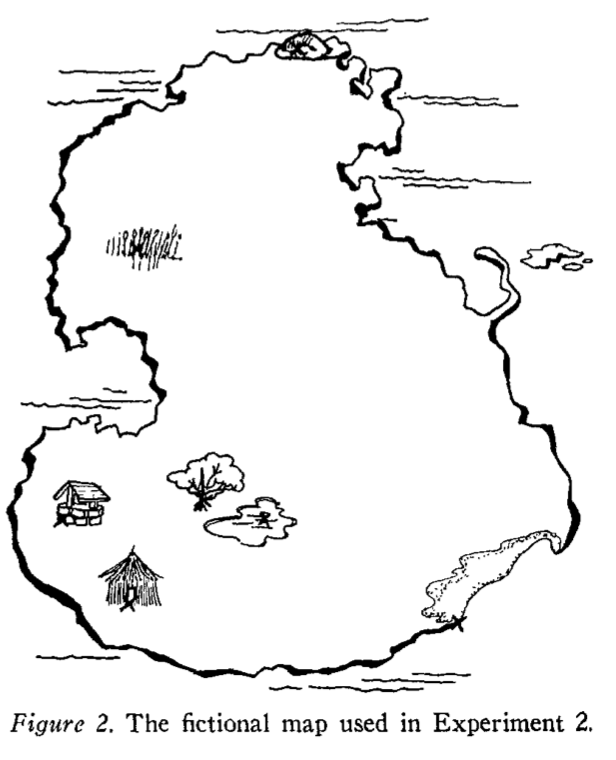
\includegraphics[width=1\linewidth]{imgs/KosslynEtAl1978Fig2}

The map was taken away and participants were asked to mentally image the map in their mind's eye. Then, the main task began. The task was split up into individual trials where the participant was asked to focus on one of the depicted locations on their mental image of the map (by imagining a black dot on top of it), and then mentally scan to a different location by moving their imagined black dot to the new location. For example, you might focus on the tree and the scan to the grass (a longer distance); or focus on the hut and scan to the lake (a shorter distance). Importantly, the researchers measured the time taken to make each scan. The empirical question was whether or not the amount of time to mentally scan from one imagined location to another would depend on the distance between the imagined locations.

Before we look at the actual data, let's consider three ways the experiment could have turned out. First, let's assume that people can scan between different locations immediately without taking any time at all, I will call this the ``no-time'' hypothesis. Second, let's assume that people will take some random amount of time to scan between the locations, the ``random-time'' hypothesis. And third, let's assume that people's scanning times will increase with the distance between the imagined locations, the ``distance-time'' hypothesis. Each of the these hypotheses makes a different prediction about how the results might turn out. Consider the three graphs below which show predictions for each hypothesis. These are examples of how the results could have turned out according to each hypothesis

\begin{figure}
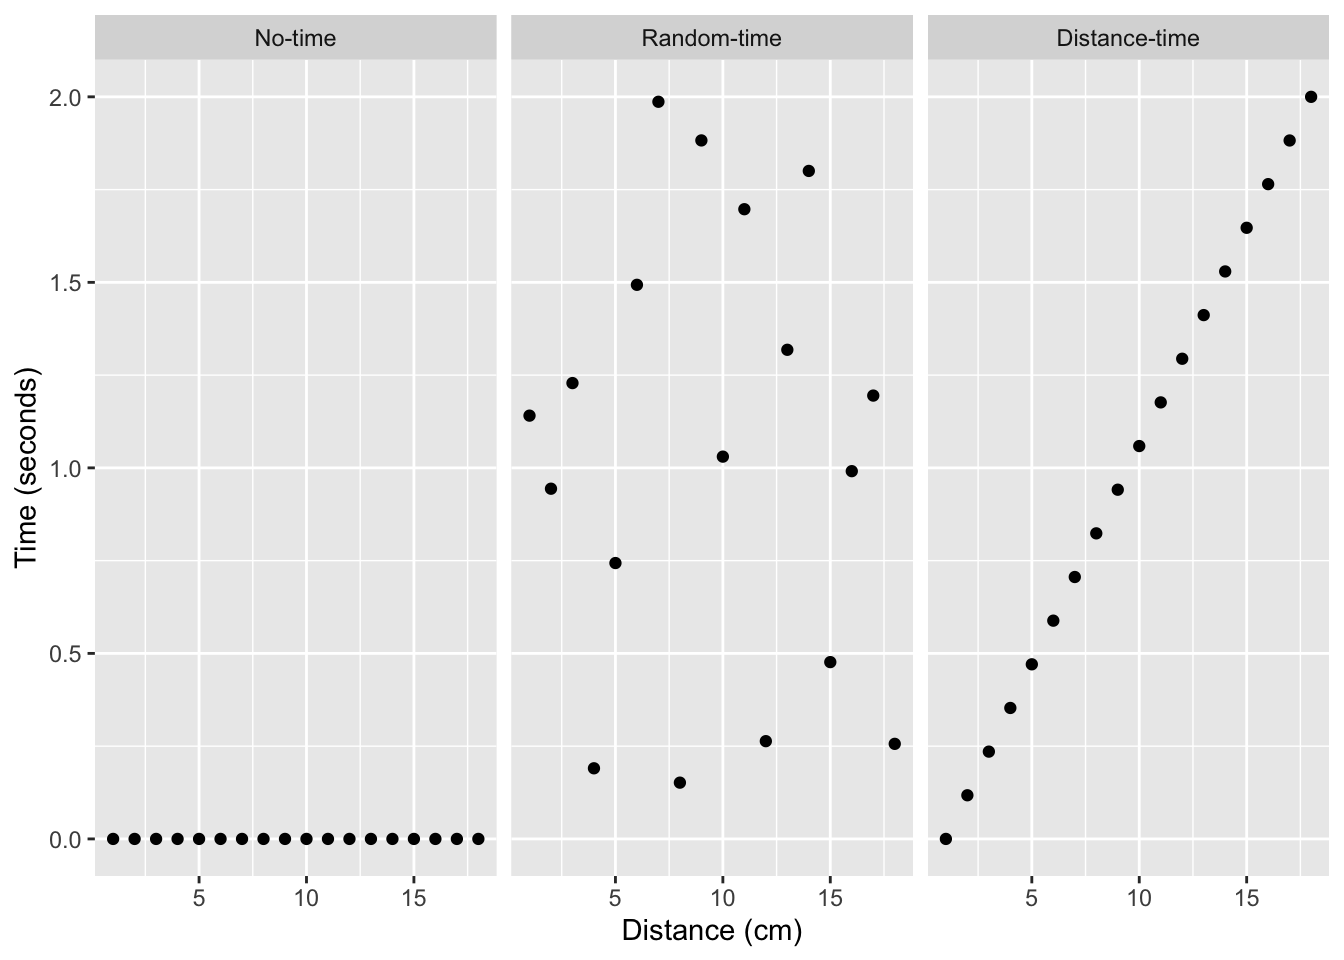
\includegraphics[width=1\linewidth]{C2_Mental_Imagery_files/figure-latex/predictScanning-1} \caption{Hypothetical results of the mental scanning task for the no-time, random-time, and distance-time hypotheses}\label{fig:predictScanning}
\end{figure}

Each of the panels shows a scatter plot of possible results. The y-axis (vertical axis) represents amount of time in seconds and ranges from zero to two seconds. Dots that are near the bottom of the plot represent shorter scanning times, and dots closer to the top represent longer scanning times. The x-axis (horizontal axis) represents the distance between locations in centimeters on the real map that participants saw before they had to imagine it. Dots closer to the left of a plot represent scanning times between locations that were close together, and dots closer to the right side represent scanning times between locations that were far apart.

The ``no-time'' plot shows all of the dots in a line at the bottom, which represents 0 seconds. This is what would happen if people could instantaneously scan from any location to any other location. Even though some locations would be closer together or further apart (represented by the fact that there are dots that go all the way from 1 cm to 15 cm), all of the scanning times would be 0.

The ``random-time'' plot shows dots spread about randomly. When I drew this graph, I had my computer pick random numbers. This is what would happen if people do take different amounts of time to scan between locations, but the amount of time would be unpredictable, and it would not depend on the distance between the imagined locations. People might be fast or slow to scan between locations that were close or far apart, and scanning speed could fluctuate based on other factors like how motivated or sleepy people were.

Finally, the ``distance-time'' plot shows dots in a tilted line (going from the bottom left to the top right) showing a positive relationship or correlation between distance and time. This is what could happen if the distance between imagined locations influences scanning time in a systematic way. Specifically, this graph shows a linear relationship. As the distance between locations increases, so does scanning time. Shorter distances take less time, and longer distances take more time.

What were the results of the study, and did they look like any of the hypothetical results that we just discussed? The original results are shown below:

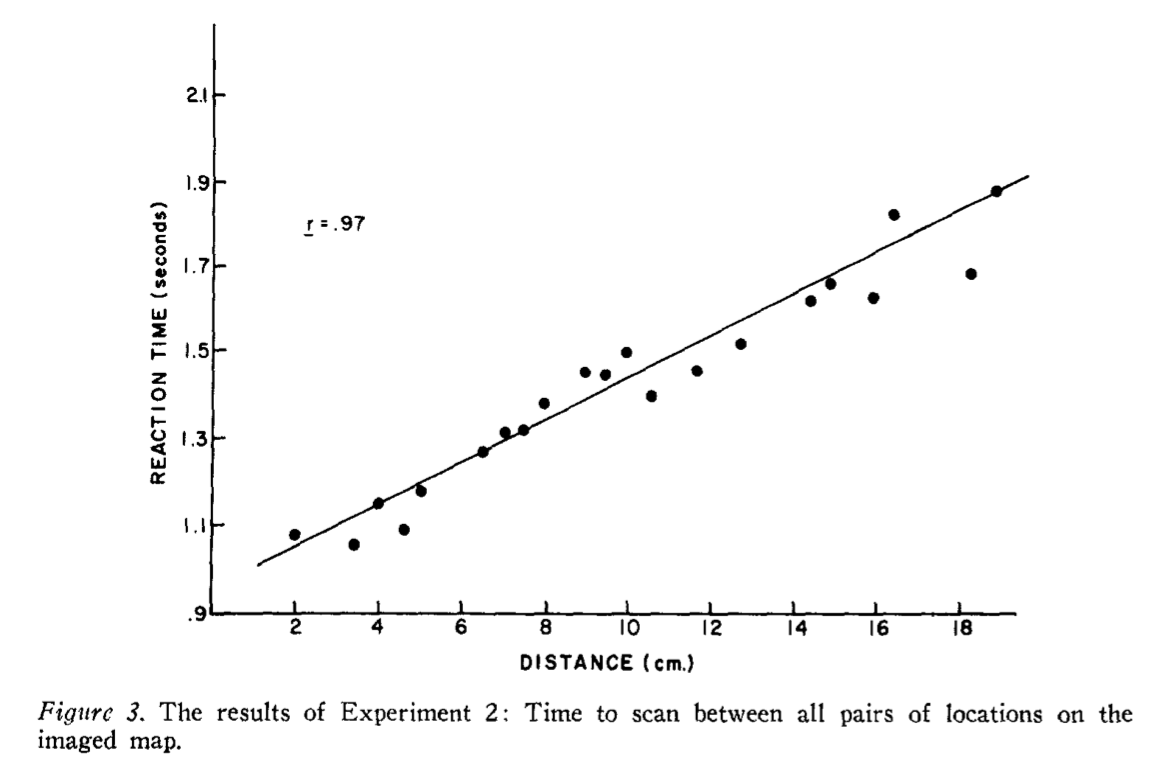
\includegraphics[width=1\linewidth]{imgs/KosslynEtAl1978Fig3}

The dots represent average scanning times between specific locations for all of the participants, and they mostly fall on the straight line. To me, the results look most like the hypothetical ``distance-time'' results. The data points are a little bit noisy, and they don't fall precisely on the line every time, so there is a bit of randomness or variability in mental scanning time too. But overall, people appear to take longer to scan between imagined locations on the map as the distance between the locations increases.

Before considering what these results could mean for theories of mental representation, let's note that this study made an attempt at advancing how mental imagery could be investigated using more objective behavioral measures. In this case, the measurement of time to make a mental scan was directly observable. Although directly observable measures of behavior have many desirable properties, including the possibility that multiple observers can mutually confirm and reach consensus on what they are observing, there are also big limitations when it comes to cognition. The biggest limitation is that direct measures of behavior are not direct measures of cognitive processes. The assumption is that cognitive processes are involved in producing the behavior in question, and that measures of behavior therefore indirectly reflect the underlying mechanisms of the mind causing the behavior. So, when someone measures ``mental scanning time'', we are only measuring the time associated with whatever happened during ``mental scanning''. The measure of time does not directly show whether or not a mental image is like a picture or a proposition. Instead, a common strategy in cognitive research is to theorize about how cognitive processes might work, and attempt to explain how those cognitive processes would result in the observable measures of behavior.

\hypertarget{explaining-mental-scanning-times}{%
\subsection{Explaining mental scanning times}\label{explaining-mental-scanning-times}}

Let's assume that Kosslyn et al's results can be trusted as a fact, and that when people scan a mental image it really does take longer to scan across longer than shorter distances in the mental image. What does this factoid tell us about the nature of mental representation? Perhaps a better question is, how are factoids like this one used in cognitive research to generate knowledge about cognitive processes?

One strategy involves inventing theories and hypotheses about cognition, and then evaluating whether or not they can predict, anticipate, and/or explain the patterns of measurements found by experiment. If a theory can explain a finding maybe it is correct. If a theory can not explain a finding, maybe it is wrong and should be discarded. Over time the process of theory building and testing would lead to a great many discarded theories that couldn't explain the findings, and what would be left could be plausible working theories that do a pretty good job explaining the findings. This characterization of how the scientific method incrementally hones in on better explanations is connects with issues in the philosophy of science,\footnote{E.g., \protect\hyperlink{ref-popperLogicScientificDiscovery1959}{Popper, K. (1959). \emph{The logic of scientific discovery}. {(First English Edition) Hutchinson \& Co}}.} which I will elaborate on over the book.

Let's finish this section by returning to the distinction between pictorial and propositional mental representations, and ask whether the pattern of data is consistent or inconsistent with either of those ideas.

\hypertarget{a-pictorial-explanation-of-scanning-time}{%
\subsubsection{A pictorial explanation of scanning time}\label{a-pictorial-explanation-of-scanning-time}}

Are the findings consistent with the assumption that people have picture-like mental representations of visual images? I don't think this question can be answered without first speculating more about how pictorial representations might work, and how they could lead to the results reported by Kosslyn et al.~Here's a simple metaphorical elaboration. I could propose that mental imagery for visual images is like perception for visual scenes, and that because of this relationship, mental imagery should behave in similar ways to visual perception. For example, objects in visual scenes have spatial distances between them, and by analogy mental images of scenes should preserve the spatial distances between imaginary objects. When looking from one object to another in the real world, it can takes time to move your eyes, and the amount of time naturally depends on how far the eyes need to move. If the metaphor holds, it is possible that mentally scanning an image will behave in the same way. So, my answer is yes. The findings could be consistent with the pictorial mental representation assumption, but only if I created a story that established how this assumption would work.

\hypertarget{a-propositional-explanation-of-scanning-time}{%
\subsubsection{A propositional explanation of scanning time}\label{a-propositional-explanation-of-scanning-time}}

Let's ask whether the results are consistent with the propositional assumption about mental representations. Pylyshyn argued that Kosslyn's results could be explained without assuming any role for pictorial mental representations. Again, to consider the propositional assumption we need to embed it into a working hypothesis about how people use propositional knowledge. First, consider how propositions could be used to code relations between objects in the scene. I will use sentences as an example of combining abstract symbols (words) to represent relations between objects in the scene.

\begin{enumerate}
\def\labelenumi{\arabic{enumi}.}
\tightlist
\item
  The island contains objects
\item
  The rock is on the north end of the island
\item
  The grass is on the north-west side of the island.
\item
  The grass is south-west of the rock
\item
  The tree is south of the grass, in the southwest of the island
\item
  The well is due west of the tree
\item
  The hut is just south of well
\item
  The lake is close to the tree, just to the southeast
\end{enumerate}

The next step is to consider how people might rely on propositions during the mental scanning task. For example, maybe the time to mentally scan between one object and another actually reflects the time it takes to activate knowledge about different objects in the propositional network. Lake and tree are close in the image, but they are also coded together in the same proposition, which could make it easier to go from the lake concept to the tree concept. Similarly, the rock is far from the tree in the image, but the way I wrote the propositions, rock is not directly coded in relation to the tree, but that relation can be established by moving through multiple propositions: the tree is south of the grass, and the grass is south-west of the rock. It might take more time to scan longer distances in the mental image because of the requirement to process multiple propositions.

As an aside, given that we have learned about aphantasia (people with no mental imagery), I wonder how aphantasics would perform in Kosslyn's task--if mental imagery is not required to perform the task, maybe they would be just fine and show the same results as everyone else\ldots or maybe they would refuse to do the task because they would be unable to imagine the map.

\hypertarget{evaluating-the-explanations}{%
\subsubsection{Evaluating the explanations}\label{evaluating-the-explanations}}

Near the beginning of this chapter I suggested that the cognitive sciences are interested in explaining how cognition works. Throughout this book we will examine how the research process is used to construct explanations about how cognition works. There are different approaches to explanation, and some of the explanations will be more or less satisfying than others. I would like to briefly evaluate the kind of explanations that I just discussed to explain the mental scanning time results. For example, there are some ways in which I find the pictorial and propositional explanations satisfying and unsatisfying. And, talking about this a little bit should help us focus on useful features of the research process that push the cognitive sciences forward. However, I think a quick detour is necessary to prepare us with some basic concepts about theories and explanations, and how they can be tested.

\hypertarget{society-and-historical-context}{%
\section{Society and Historical context}\label{society-and-historical-context}}

One outgrowth of the mental imagery research we discussed was the creation of the website \url{aphantasia.com}, where many people from across the world are creating an online community to discuss and learn more about their own extreme differences in mental imagery abilities. This is a great example of people being interested in how their own cognition works, and wanting learn to more about it. For me personally, I think it would be great if research into mental imagery could help me increase how much control I have over the vividness of my mental imagery. Maybe continued research on this topic will lead to discoveries on this issue. That could be a positive development for me and other people interested in controlling the vividness of their mental imagery.

As I mentioned before, research into cognitive abilities has not always had uniformly positive implications for society, and there are examples where research applications were severely destructive for some groups of people. For example, remember Sir Francis Galton? In 1880 he published the first study showing evidence for individual differences in mental imagery. Mental imagery is a fascinating topic about how people experience their own mental life. You might assume that Galton was interested in answering questions like, ``how does mental imagery work?''. Perhaps this was part of Galton's motivation for running the study. But, I have purposefully been silent so far about other reasons why Galton ran the study. He tells us the main reason at the beginning of his paper, which reads:

``The larger object of my inquiry is to elicit facts that shall define the natural varieties of mental disposition in the two sexes and in different races, and afford trustworthy data as to the relative frequency with which different faculties are inherited in different degrees.''

Why do you think Galton was trying to measure if mental imagery is different between people? Was he trying to explain how mental imagery works?

What was going on at the time that led Galton to ask his questions about mental imagery? How did his results and larger research program influence society? Unfortunately, I should warn you that if you do not already know the answers to these questions, you may find the history deeply disturbing, I know I did.

I mentioned earlier that Galton was in the United Kingdom, and that some of his ideas tended to spread among psychologists in other countries. Galton is famous for many things because he happened to make contributions in many different fields. For example, he is involved with inventing the statistical concept of correlation.\footnote{\protect\hyperlink{ref-galtonCorelationsTheirMeasurement1889}{Galton, F. (1889). I. {Co}-relations and their measurement, chiefly from anthropometric data. \emph{Proceedings of the Royal Society of London}, \emph{45}(273-279), 135--145. \url{https://doi.org/dz5sd6}}; \protect\hyperlink{ref-stiglerFrancisGaltonAccount1989}{Stigler, S. M. (1989). Francis {Galton}'s account of the invention of correlation. \emph{Statistical Science}, 73--79. \url{https://doi.org/dg8nxj}}.} He was interested in correlation because he was interested in inheritance, especially the idea that children inherit mental abilities from their parents.\footnote{\protect\hyperlink{ref-galtonKinshipCorrelation1890}{Galton, F. (1890). Kinship and correlation. \emph{The North American Review}, \emph{150}(401), 419--431}.} And, Galton was interested in the inheritance of mental abilities because he was also the father of the eugenics movement.\footnote{\protect\hyperlink{ref-galtonHereditaryTalentCharacter1865}{Galton, F. (1865). Hereditary talent and character. \emph{Macmillan's Magazine}, \emph{12}(157-166), 318--327}, \protect\hyperlink{ref-galtonHereditaryGenius1869}{(1869). \emph{Hereditary genius}. {Macmillan}}.} Eugenics became a world-wide social movement partly interested in ``improving'' society across generations through selective human breeding programs. Eugenics programs, ideology, and social policies led to numerous historical injustices and violations of human rights and atrocities.

After spending a great deal of time learning about the lasting legacy of eugenics in society, along with the fact that the discipline of psychology played a very large role facilitating the eugenics movement; I have decided that it would be irresponsible of me to write a survey textbook on cognitive research without acknowledging the historical background of eugenics. I review this background in the next chapter, and then connect it with psychological research into cognitive abilities in the upcoming chapter on intelligence testing, as well as a few other aspects of cognitive research throughout the textbook.

\hypertarget{eugenics-and-psychology}{%
\chapter{Eugenics and Psychology}\label{eugenics-and-psychology}}

\begin{tabular}{r|l|l}
\hline
Word Count & Reading Time & Last Compiled\\
\hline
4581 & 22.9 minutes & 2021-11-05 17:31:32 GMT\\
\hline
\end{tabular}

\hypertarget{chapter-overview-2}{%
\section{Chapter Overview}\label{chapter-overview-2}}

This chapter describes the eugenics movement and points to some its connections with the larger discipline of psychology and research into cognition. Some of these connections are expanded upon in later chapters, especially the next chapter on mental testing.

As an editorial note, throughout this chapter we will encounter descriptions of people from the perspective of eugenics. For example, eugenics differentiated people on the basis of human characteristics that eugenicists decided were desirable or undesirable. As a result, people who had eugenically desired traits were labelled as ``high-quality'' or ``superior'' compared to people who had eugenically undesired traits, who were labelled as ``low-quality'' or ``inferior''. These and other similar descriptors of human beings will sometimes be used in this chapter for the purpose of describing de-humanizing aspects of eugenics ideology.

\hypertarget{eugenics-psychology-and-the-cognitive-sciences}{%
\section{Eugenics, psychology and the cognitive sciences}\label{eugenics-psychology-and-the-cognitive-sciences}}

Including a chapter about eugenics is not very common in introductory psychology textbooks. When I learned about histories of psychology and cognitive psychology the topic of eugenics was rarely discussed. One reason for the lack of coverage might be that cognitive psychology and the cognitive sciences became established academic disciplines well after the primary eugenics movements had come and gone; and, eugenics may be viewed as ``ancient history'' or irrelevant to discussions of modern day cognitive sciences. I share the view that the rise and gradual fall of the eugenics movement is inextricably intertwined with psychology especially between the turn of the 20th century (1890s-ish) and 1950s (ish).\footnote{\protect\hyperlink{ref-yakushkoEugenicsItsEvolution2019}{Yakushko, O. (2019a). Eugenics and its evolution in the history of western psychology: {A} critical archival review. \emph{Psychotherapy and Politics International}, \emph{17}(2). \url{https://doi.org/gg3hsf}}.} Although the modern cognitive sciences were established between the 1950s and 1980s, research into cognitive abilities had been ongoing for decades prior to the so-called ``cognitive revolution''. The eugenics movement substantially influenced early branches of research into cognitive abilities, and shaped the kinds of questions, tools/methods, and applications that the research enterprise held for society, and the development of the cognitive sciences, then and now.

Last chapter we learned that Sir Francis Galton was interested in mental abilities because of his research into individual differences in the vividness of mental imagery. However, throughout the chapter I did not elaborate on the fact that Galton was also interested in Eugenics, which motivated him conduct the research in the first place.

What was the Eugenics movement? How did it get started, what did it do, when did it end? I will address these questions in this chapter. How was psychology involved? And what does eugenics have to do with cognition? I will attempt to establish these connections in the next chapter, and to a lesser extent the remaining chapters.

\hypertarget{eugenics-an-overview}{%
\section{Eugenics: an overview}\label{eugenics-an-overview}}

Here is a brief overview of eugenics. Galton published on eugenics as early as 1865.\footnote{\protect\hyperlink{ref-galtonHereditaryTalentCharacter1865}{Galton, 1865}.} Eugenics transitioned from ideas about ``improving society'' in journal pages read by small groups of academics elites, into a large and complex social movement that was broadly accepted-- from everyday citizens to national leaders-- in numerous countries around the world\footnote{\protect\hyperlink{ref-kuhlBettermentRaceRise2013}{Kühl, S. (2013). \emph{For the {Betterment} of the {Race} - {The Rise} and {Fall} of the {International Movement} for {Eugenics} and {Racial Hygiene}}. {Palgrave Macmillan}. \url{https://www.palgrave.com/gp/book/9781137286116}}.} up until the 1940s and 50s.

A basic idea in eugenics was that society could be improved and its problems solved by selectively breeding humans just like other animals. Eugenicists assumed that traits they considered desirable, like human ``intelligence'', were inherited from parents; and, they argued that society as a whole could be made more intelligent over generations by breeding more intelligent people with each other. Similarly, eugenicists assumed that traits they considered undesirable, like ``feeble-mindedness'' \footnote{a generic word commonly used to describe mental illness}, were inherited from parents; and they argued that society as a whole could eliminate undesirables over generations by preventing people deemed undesirable from having offspring.

The eugenics movement established itself in many countries and sought to enact social polices to forward the aims of the eugenics movement. Their policies were responsible for many human rights violations and atrocities. The legacy of eugenics campaigns has left lasting impacts on society that continue today.

The early discipline of psychology was complicit in eugenics, and large numbers of psychologists were eugenicists. The general involvement of psychology reflects the widespread acceptance of eugenics in society (psychology wasn't special in this regard). It was the specific aspects of psychology's involvement that warrants the descriptor ``complicit''.

Eugenics needed ways to ``scientifically'' measure physical and mental qualities of individual people. Psychologists helped create and deploy the tests of human ability (e.g., intelligence tests, see next chapter) that would be used to carry out eugenics campaigns on society. Research concerned with cognitive abilities was motivated and deeply entrenched in eugenics for well over half a century (1900s-1950s). The cognitive sciences did not emerge unscathed from this historical backdrop while advancing attempts to explain how cognitive abilities work, and connections to cognitive science are mentioned in upcoming chapters.

\hypertarget{galtons-eugenics}{%
\section{Galton's Eugenics}\label{galtons-eugenics}}

Eugenics was a potent mix of ideas ranging from scientific claims, social policy, religion, and visions of Utopia. Although eugenics ideology morphed over time and geographical place,\footnote{\protect\hyperlink{ref-bashfordOxfordHandbookHistory2010}{Bashford, A., \& Levine, P. (Eds.). (2010). \emph{The {Oxford Handbook} of the {History} of {Eugenics}}. {Oxford University Press}. \url{https://doi.org/10.1093/oxfordhb/9780195373141.001.0001}}.} the basic tenets of the movement are still captured well by Galton's early writings. In 1865, Galton wrote ``Hereditary talent and character,''\footnote{\protect\hyperlink{ref-galtonHereditaryTalentCharacter1865}{Galton, 1865}.} a short paper that was expanded to a book a few years later, ``Hereditary Genius.''\footnote{\protect\hyperlink{ref-galtonHereditaryGenius1869}{Galton, 1869}.} These works describe Galton's ideas about human quality-- that some humans are much more superior in quality than others-- his research claiming that the most important human qualities are hereditary (biologically inherited from parents), his fears that society was degrading all around him, and his plan to save society by creating a new scientific religion capable of engineering a supreme human race over generations, simply by controlling human reproduction.

Galton referenced the practice of dog breeding, which involves selectively mating dogs with particular physical and behavioral traits over generations of broods. Dog-breeding was a choice example, because it would have been obvious to anyone that breeding over generations can produce dramatic results: all of the many different dog breeds have been achieved through breeding. One of Galton's radical claims for the time, was that breeding should be used on humans, just like dogs, and that breeding programs would be a simple, straightforward, and already well-understood method to produce a superior race of humans over generations.

Galton's eugenics ideas did not appear in a vacuum, and they were influenced by the scientific and social context he was working in. Galton's eugenics writings appeared just after 1859, when his cousin Charles Darwin published the theory of evolution in the \emph{Origin of the species}.\footnote{\protect\hyperlink{ref-darwinOriginSpecies1859}{Darwin, C. (1859). \emph{The origin of species}. {John Murray, Albemarle Street}}.} Darwin's theory, described how animal species evolved over time through a process of natural selection, and continues to stand today as a powerful explanatory theory of life on earth. This same time period included threats to British imperialism and efforts by many nations to establish dominance and socio-cultural order across the globe. Galton was an esteemed upper-class British man of science (eventually knighted in 1909), who held sexist and racist views common among his peers. For example, long before genetics would show that there is no biological basis for race,\footnote{\protect\hyperlink{ref-yudellTakingRaceOut2016}{Yudell, M., Roberts, D., DeSalle, R., \& Tishkoff, S. (2016). Taking race out of human genetics. \emph{Science}, \emph{351}(6273), 564--565. \url{https://doi.org/gfkndx}}.} academics like Galton assumed that people from ``uncivilized'' countries were of much lower quality than people from ``civilized'' countries, and that these differences must have evolved, and must be heritable. Furthermore, in the tradition of \href{https://en.wikipedia.org/wiki/Thomas_Robert_Malthus}{Thomas Malthus} -- who is famous for speculating about the imminent collapse of society as a result of population growth-- Galton feared that society would deteriorate over the generations due to increased global interactions between people across the world. Specifically, Galton feared that ``natural selection'' left to chance would allow inferior, low-quality and uncivilized people to reproduce, pollute the gene pool, spread inferior genes across the world, and cause the slow decline and ultimate destruction of the human race.

Galton saw eugenics as a way to arrest human destiny from natural selection, and use the new powers of science and technology to save humanity from itself. Eugenics was not only about improving society for one generation, it would be sold as a quasi-religious movement dedicated to improving humanity across generations, for the rest of time. Although improving humanity might not seem like a frightening goal, it is worth considering questions like: What is being improved? Who get's to decide what needs improving? What kinds of changes count as improvement? Who will benefit from the improvement? Will the costs of improvement be shared equally? In answering these questions, the eugenics movement argued that improving humanity meant identifying and eliminating eugenically low quality humans from the species; which is a frightening prospect for large groups of people who were dehumanized by eugenicists.

\hypertarget{the-eugenics-movement}{%
\section{The Eugenics movement}\label{the-eugenics-movement}}

Galton's eugenics ideas could have stayed on the page like most dystopian science fiction novels, but unfortunately they took on a life of their own. In this section, we establish the scale of eugenics by examining its dimensions as a social movement.

\hypertarget{a-timeline}{%
\subsection{A Timeline}\label{a-timeline}}

The eugenics movement spread from Britain around the world and impacted different countries in similar and unique ways. For a very informative timeline on major events in the eugenics movement take a look at the \href{https://eugenicsarchive.ca/discover/timeline}{interactive timeline} created by the Canadian funded \href{https://eugenicsarchive.ca/}{eugenics archive} project. Although the timeline includes many events relevant to Canada's eugenics legacy, it also provides comprehensive coverage of important historical events in eugenics movements worldwide.

\hypertarget{from-ideas-to-internationalization}{%
\subsection{From ideas to internationalization}\label{from-ideas-to-internationalization}}

Galton continued to expand and popularize his ideas from 1865, and coined the phrase eugenics in 1883.\footnote{\protect\hyperlink{ref-galtonInquiriesHumanFaculty1883}{Galton, F. (1883). \emph{Inquiries into human faculty and its development}. {Macmillan}}.} In these few decades eugenics proponents had succeeded in blaming an array of social problems on diverse groups of people labelled as undesirable and inferior, on the basis of characteristics like skin color, ethnicity, and mental illness or disability. Furthermore, these undesirable characteristics were argued by eugenicists to be heritable traits. Eugenics promoted fears that hoards of undesirable people were breeding and spreading their undesirable traits throughout society, and that society would ultimately degenerate and collapse unless actions proposed by eugenicists were taken to save society.

By 1882, fear of undesirables spread to American immigration policy, and immigrants who were found to be ``undesirable'' could be denied entry to the USA.\footnote{\protect\hyperlink{ref-bayntonDefectivesLandDisability2005}{Baynton, D. C. (2005). Defectives in the land: {Disability} and {American} immigration policy, 1882-1924. \emph{Journal of American Ethnic History}, \emph{24}(3), 31--44}; \protect\hyperlink{ref-chenFitCitizenshipEugenics2015}{Chen, M. (2015). Fit for {Citizenship}?: {The Eugenics Movement} and {Immigration Policy}. \emph{Dissent}, \emph{62}(2), 73--86. \url{https://doi.org/gmqz7d}}.} By 1897, fear that ``degenerates'' would reproduce and overwhelm society led lawmakers in Michigan to propose a compulsory sterilization law--where the state would forcibly sterilize any woman deemed to be a degenerate. Compulsory sterilization laws were adopted by over 30 states and led to 60,000 forced sterilizations.\footnote{\protect\hyperlink{ref-EugenicsCompulsorySterilization}{\emph{Eugenics: {Compulsory Sterilization} in 50 {American States}}. (n.d.). Retrieved September 8, 2021, from \url{https://www.uvm.edu/~lkaelber/eugenics/}}.} By the early 1900s, the formal eugenics societies were being established around the world.

In Britain, Galton sat as the first president of the Eugenics Education Society in 1907. One year earlier, Charles Davenport formed a Eugenics committee in the American breeders association-- a pre-cursor to the Eugenics Record Office, which was the national headquarters of eugenics in the USA (located at Cold Springs Harbor Laboratory in Huntington, Long Island, NY).\footnote{\protect\hyperlink{ref-allenEugenicsRecordOffice1986}{Allen, G. E. (1986). The eugenics record office at {Cold Spring Harbor}, 1910-1940: An essay in institutional history. \emph{Osiris}, \emph{2}, 225--264. \url{https://doi.org/fqthgg}}.} Eugenics societies spread across the world. The Oxford handbook of the history of eugenics,\footnote{\protect\hyperlink{ref-bashfordOxfordHandbookHistory2010}{Bashford \& Levine, 2010}.} has individual chapters describing the aftermath of eugenics in Britain, South Asia, Australia and New Zealand, China and Hong Kong, South Africa, Colonial Kenya, Germany, France, the Netherlands and the Dutch East Indies, the Scandinavian States, Southern Europe, Eastern Europe, Russia and the Soviet Union, Japan, Iran, the Jewish Diaspora; Cuba Puerto, Rico, and Mexico; Brazil, the United Sates, and Canada.

\hypertarget{conferences-and-popularity}{%
\subsection{Conferences and popularity}\label{conferences-and-popularity}}

\begin{floatright50}
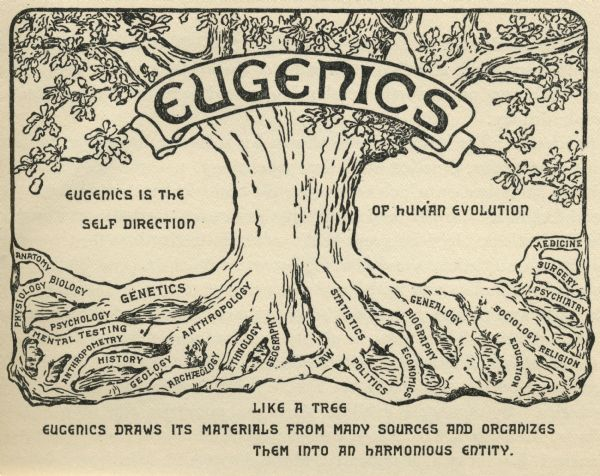
\includegraphics[width=1\linewidth]{imgs/Eugenics_tree}

\end{floatright50}

There were many national and international conferences where elites in the eugenics movement gathered to popularize and discuss eugenical solutions to improve society. For example, the first national conference on race betterment was held in Battle Creek Michigan in 1914 \footnote{the conference proceedings are available from internet archive \url{https://archive.org/details/proceedingsoffir14nati}}. The first (1912), second (1921) and third (1932) International Eugenics Congresses were held in London, and New York (last two). The tree of eugenics was created for the second conference and depicts how the movement saw itself as, ``the self-direction of human evolution'', that would harmoniously integrate many fields of study for the purpose of bettering mankind. Just like each of the countries listed at the end of the last section, the academic fields listed in the roots of the tree of eugenics also have their own eugenics legacies to contend with.

In America, eugenics appealed to large segments of society and was embraced by celebrities, national leaders, and everyday people across country. Some famous Americans who were strong proponents of eugenics include Alexander Graham Bell (inventor of the telephone), John Harvey Kellogg (Kellog's Corn Flakes), and Theodore Roosevelt (American President). During the height of its activity, the Eugenics Record Office trained scores of operators to disseminate information about eugenics across the states. For example, it would be common to attend a county fair and learn about eugenics at a eugenics information tent. Or, to participate in eugenics contests, like the ``better babies'' contests, where families had their baby's judged and won prize for having the highest quality baby (by eugenical standards).\footnote{\protect\hyperlink{ref-seldenTransformingBetterBabies2005}{Selden, S. (2005). Transforming better babies into fitter families: {Archival} resources and the history of the {American} eugenics movement, 1908-1930. \emph{Proceedings of the American Philosophical Society}, 199--225}.} The take home message here is that the eugenics movement was highly organized and its proposals for improving society were very well known, commonly accepted, and fanatically embraced by its strongest adherents.

\hypertarget{eugenics-journals}{%
\subsection{Eugenics Journals}\label{eugenics-journals}}

As the tree of eugenics shows, the movement thought of itself as the culmination of many academic disciplines. Although eugenics did not succeed in perpetuating itself as a new academic department, it claimed to be a science for many years, and established academic journals and related publications. A few English language eugenics journals include: \href{https://www.ncbi.nlm.nih.gov/pmc/journals/1186/}{The Eugenics Review}, The Eugenical News \footnote{several volumes are available on the internet archive \url{https://archive.org/search.php?query=Eugenical\%20News}}, \href{https://www.jstor.org/journal/jracedeve}{The Journal of Race Development} (whose first editor was the first president of the American Psychological Association, Granville Stanley Hall), and the \href{https://onlinelibrary.wiley.com/toc/20501439/1925/1/1}{Annals of Eugenics} (which was renamed Annals of Human Genetics).

It is highly informative, eye-opening, and even terrifying to read through the papers in these journals. One notable feature of the journals was that the eugenics enterprise was not hidden, but visible and open to the reading public. This allows unusual access to the history of the movement because the development of eugenical ideology, and its claims and methods for influencing society are all written down in the journals, books, conference proceedings, and other propaganda (including textbooks, pamphlets, and movies). Some of the eugenics journals stopped publishing, and others renamed themselves (and continue to publish) after the eugenics movement became socially unacceptable.

\hypertarget{eugenics-fears}{%
\subsection{Eugenics Fears}\label{eugenics-fears}}

Fear of people on the margins of society was a common feature of eugenics movements across countries. Fear was created in two ways. First, fear was created by sub-humanizing already marginalized groups of people, labeling them as mentally and physically inferior, and using adjectives like, degenerate, impure, and moral monsters, to underline the message. Many different groups of people were targeted by eugenics and deemed unfit, from people with physical and mental disabilities, to immigrants, and people with different colored skin from the dominant eugenics movement in a particular country. In majority white countries like Britain, Germany, Canada, Australia, and the United States, the eugenics movement forwarded an agenda of white supremacy and reinforced existing forms of racism against non-whites. Non-white citizens were deemed inferior, and a common strategy was to fabricate scientific evidence showing that white people were superior in terms of eugenically desired traits (like intelligence) compared to non-whites.

Second, eugenicists suggested that marginalized groups of people would cause the collapse of society. The following characterization of ``eugenics logic'' is similar to what you might read in eugenics propaganda: ``Inferior people are inferior because they have inferior genes. Inferior people pass on their inferior genes to their offspring when they have children, and they create inferior children with inferior genes. Also, many disgusting and inferior moral degenerates reproduce at very high rates. Society is deteriorating as we speak because so many inferior people are breeding, and society as we know it will collapse unless we follow eugenics solutions to the problem.''

\hypertarget{positive-and-negative-eugenics}{%
\subsection{Positive and Negative Eugenics}\label{positive-and-negative-eugenics}}

Eugenics promised scientific solutions to the problems it identified in society, and presented itself as a progressive social movement. Eugenicists distinguished between positive and negative eugenics as two general directions that would help improve the human race across generations through breeding.

Positive eugenics were ostensibly methods that would increase or encourage reproduction between high quality people (as determined by eugenics values). Negative eugenics involved methods for decreasing reproduction between low quality people (as determined by eugenics values). In practice, eugenics methods increased inequalities in society-- positive eugenic methods gave more privileges to already powerful and privileged groups, and negative eugenic methods took away privileges from already marginalized groups, and worse. Wide-ranging positive and negative eugenics policies were deliberately deployed in many countries for many decades, and remnants of these policies continue to influence modern society in many ways. The following quote from Galton in 1883\footnote{\protect\hyperlink{ref-galtonInquiriesHumanFaculty1883}{Galton, 1883}.} was prescient in describing the many ways that eugenicists attempted to influence society with their social policies.

\begin{quote}
``a brief word to express the science of improving stock, which is by no means confined to questions of judicious mating, but which, especially in the case of man, takes cognizance of all influences that tend in however remote a degree to give to the more suitable races or strains of blood a better chance of prevailing speedily over the less suitable than they otherwise would have had (Galton, 1883, p.17)''
\end{quote}

The next section lists some of the eugenics policies that had lasting impacts on society.

\hypertarget{influences-on-society}{%
\section{Influences on society}\label{influences-on-society}}

Because eugenics was so widespread and common in many countries for a very long time, it had the opportunity to influence society in numerous and sometimes unexpected ways. Here is a short list.

\hypertarget{eugenics-and-mental-health}{%
\subsection{Eugenics and Mental health}\label{eugenics-and-mental-health}}

Eugenics ideology shaped the history of mental health treatment.\footnote{\protect\hyperlink{ref-dowbigginKeepingAmericaSane1997}{Dowbiggin, I. R. (1997). \emph{Keeping {America Sane}: {Psychiatry} and {Eugenics} in the {United States} and {Canada}, 1880-1940}. {Cornell University Press}. \url{https://books.google.com?id=tMTJG0E4PPMC}}; \protect\hyperlink{ref-fischerMaltreatmentPeopleSerious2012}{Fischer, B. A. (2012). Maltreatment of people with serious mental illness in the early 20th century: A focus on {Nazi Germany} and eugenics in {America}. \emph{The Journal of Nervous and Mental Disease}, \emph{200}(12), 1096--1100. \url{https://doi.org/f4f3pz}}; \protect\hyperlink{ref-thomsonDisabilityPsychiatryEugenics2010}{Thomson, M. (2010). Disability, psychiatry, and eugenics. \emph{The Oxford Handbook of the History of Eugenics}, 116--133}.} People with mental illness were treated as genetically inferior, and negative eugenics was used to prevent people with mental illness from reproducing. One strategy was to institutionalize patients in mental hospitals that were in distant locations--which would prevent them from breeding with the general public. Another strategy was to forcibly sterilize patients against their will to ensure they could never reproduce. For example, the United States passed compulsory sterilization laws for ``defectives'' in over 30 states.

\hypertarget{eugenics-and-racism}{%
\subsection{Eugenics and Racism}\label{eugenics-and-racism}}

Eugenics reinforced existing forms of racism in several ways. White eugenicists were concerned that the ``white race'' would degenerate if it mixed with ``inferior'' non-white races. In America, eugenicists supported increased segregation between whites and blacks, which would limit inter-marriage; and, they supported miscegenation laws to make inter-marriage illegal.\footnote{\protect\hyperlink{ref-lombardoMiscegenationEugenicsRacism1987}{Lombardo, P. A. (1987). Miscegenation, eugenics, and racism: {Historical} footnotes to {Loving} v. {Virginia}. \emph{UC Davis L. Rev.}, \emph{21}, 421}.}

\hypertarget{eugenics-and-fertility-control}{%
\subsection{Eugenics and Fertility control}\label{eugenics-and-fertility-control}}

Eugenics was highly concerned with fertility control issues. As a result, eugenics overlapped with other progressive movements, such as the womens movement to legalize abortion. For example, Margaret Sanger, the founder of planned parenthood, was also a eugenicist. Abortion would be a welcome tool for eugenics because it could be used to terminate pregnancies resulting in eugenically ``defective'' or inferior offspring. Margaret Sanger, like other eugenicists at the time in America, was also involved in the white supremacy movement, and promoted her views by giving talks to white supremacy groups. Many modern institutions and organizations have eugenic legacies in their past, and it is notable that planned parenthood has recently begun publicly acknowledging and reckoning with this history.\footnote{\protect\hyperlink{ref-johnsonOpinionHeadPlanned2021}{Johnson, A. M. (2021, April 17). Opinion \textbar{} {I}'m the {Head} of {Planned Parenthood}. {We}'re {Done Making Excuses} for {Our Founder}. \emph{The New York Times: Opinion}. \url{https://www.nytimes.com/2021/04/17/opinion/planned-parenthood-margaret-sanger.html}}; \protect\hyperlink{ref-plannedparenthoodStatementMargaretSanger2020}{Parenthood, P. (2020). \emph{Statement about {Margaret Sanger} and {Planned Parenthood}'s mission}. \url{https://www.plannedparenthood.org/planned-parenthood-north-central-states/about-ppncs/media-relations/statement-about-margaret-sanger-and-planned-parenthoods-mission}}.}

\hypertarget{eugenics-and-education}{%
\subsection{Eugenics and Education}\label{eugenics-and-education}}

Eugenics was involved in American education in numerous and sometimes unexpected ways. Eugenicists spread their views in schools through textbooks, such as high school biology textbooks, that reinforced eugenics beliefs and ideas.\footnote{\protect\hyperlink{ref-seldenInheritingShameStory1999}{Selden, S. (1999). \emph{Inheriting shame: {The} story of eugenics and racism in {America}}. {Teachers College Press}}.} Gifted school programs were born out of positive eugenics to develop eugenically ``superior'' children,\footnote{\protect\hyperlink{ref-mansfieldGiftednessPropertyTroubling2015}{Mansfield, K. C. (2015). Giftedness as property: {Troubling} whiteness, wealth, and gifted education in the {US}. \emph{International Journal of Multicultural Education}, \emph{17}(1), 121. \url{https://doi.org/gg47h8}}.} and concerns about racial bias for admission to these programs remain current \footnote{for example, the serial podcast nice white parents discusses a modern history and concerns of bias in gifted school programs in New York City \url{https://www.nytimes.com/2020/07/23/podcasts/nice-white-parents-serial.html}}. Standardized testing in education was created and proliferated by psychologists who were committed to the cause of eugenics, such as \href{https://en.wikipedia.org/wiki/Carl_Brigham}{Carl Brigham} a psychologist and eugenicist who was hired by the College Board to create the \href{https://en.wikipedia.org/wiki/SAT}{SAT}. \href{https://en.wikipedia.org/wiki/Edward_Thorndike}{Edward Thorndike}, sometimes lauded as the father of educational psychology, was a prominent eugenicist who wanted to use education for purposes of eugenics. Even the playground movement, which advocated for schools to include playgrounds, was mired in eugenics.\footnote{\protect\hyperlink{ref-mobilyEugenicsPlaygroundMovement2018}{Mobily, K. E. (2018). Eugenics and the playground movement. \emph{Annals of Leisure Research}, \emph{21}(2), 145--160. \url{https://doi.org/gg4652}}.}

An example of the continuing trauma from eugenics policies in education\footnote{\protect\hyperlink{ref-chapmanColonialismDisabilityPossible2012}{Chapman, C. (2012). Colonialism, disability, and possible lives: {The} residential treatment of children whose parents survived {Indian Residential Schools}. \emph{Journal of Progressive Human Services}, \emph{23}(2), 127--158. \url{https://doi.org/gmq2n5}}.} comes from \href{https://en.wikipedia.org/wiki/Canadian_Indian_residential_school_system}{Canada's residential school system}. These schools were in mandatory operation from 1894 to 1947, and the last one closed in 1996. In this boarding school system indigenous children were separated from their parents ostensibly for the purpose of assimilating them into Canadian culture. Eugenics policies included the practices of segregation and institutionalization (by sending the children to remote locations); and, many indigenous female students were involuntary sterilized.\footnote{\protect\hyperlink{ref-pegoraroSecondrateVictimsForced2015}{Pegoraro, L. (2015). Second-rate victims: {The} forced sterilization of {Indigenous} peoples in the {USA} and {Canada}. \emph{Settler Colonial Studies}, \emph{5}(2), 161--173. \url{https://doi.org/gmq2pm}}.} Child abuse was rampant. In 2021, the remains of children in unmarked gravesites were discovered on the grounds of several residential schools across Canada, with victims numbering in the thousands. The Canadian government is attempting reconciliation for survivors, families, and communities affected by the residential school system through the \href{https://www.rcaanc-cirnac.gc.ca/eng/1450124405592/1529106060525}{Truth and Reconciliation Commission}.

\hypertarget{eugenics-and-genocide}{%
\subsection{Eugenics and Genocide}\label{eugenics-and-genocide}}

One of the most notorious outcomes of the eugenics movement occurred in Germany during world war II. While America had its eugenics societies, like the \href{https://en.wikipedia.org/wiki/Human_Betterment_Foundation}{Human Betterment Foundation}, Germany's eugenic movement had established itself beginning in 1905 as ``Deutsche Gesellschaft für Rassenhygiene'', or the ``German Society for Racial Hygiene''. Here, eugenic goals included creating a purified and superior white race, and these goals were acted upon by committing atrocities like the holocaust.

The precursors of the Nazi eugenics program were already well-established by eugenicists in other countries. For example, the English statistician Karl Pearson (the inventor of Pearson's correlation co-efficient) was Galton's protege, and became the first ``Galton Chair in National Eugenics'' at the University College London, after Galton's death in 1911. Pearson used his statistics research for eugenics. To take one example, Pearson established the journal ``Annals of eugenics'' in 1925, and published a series of four lengthy (approximately 400-500 pages in total) research papers that demonstrated how to ``scientifically'' measure Jewish children and their parents to identify eugenically inferior Jews, so that the ``cold light of statistical inquiry'' could be used ultimately to stop Jewish immigration to Britain.\footnote{\protect\hyperlink{ref-pearsonProblemAlienImmigration1925}{Pearson, K., \& Moul, M. (1925). The problem of alien immigration into {Great Britain}, illustrated by an examination of {Russian} and {Polish Jewish} children. \emph{Annals of Eugenics}, \emph{1}(1), 5--54. \url{https://doi.org/cvn6gq}}.} The Nazi regime would elaborate on these publicized methods and take them to their extreme conclusion, which included the genocide of an estimated six million Jews in the holocaust, and mass killing of other groups deemed to be eugenically inferior such as homosexuals, and mentally disabled people.

The numerous Nazi war atrocities which were clearly driven by and connected to the German eugenics movement are commonly cited as a reason for the world-wide decline of the eugenics movement after world war II. In America, the previously very public eugenics movement became unpopular. Eugenics journals changed their names. Eugenics societies stopped publishing their member lists. The damaging legacy and history of eugenics movements continues to the present day, and additional coverage is beyond the scope of this chapter. For further reading on this topic consider these books.\footnote{\protect\hyperlink{ref-bashfordOxfordHandbookHistory2010}{Bashford \& Levine, 2010}; \protect\hyperlink{ref-kuhlBettermentRaceRise2013}{Kühl, 2013}; \protect\hyperlink{ref-wilsonEugenicThinking2018}{Wilson, R. A. (2018). Eugenic {Thinking}. \emph{Philosophy, Theory, and Practice in Biology}, \emph{10}(20200624). \url{https://doi.org/gg386w}}.}

\hypertarget{psychology-and-eugenics}{%
\section{Psychology and Eugenics}\label{psychology-and-eugenics}}

In the preceding sections my aim was to convey ideologies of eugenics, the tremendous scale and acceptance of eugenics across the world for at least half a century, and some of the fallout from the movement. In the last section, I briefly review some connections between psychology and eugenics, and elaborate on primary connections in the next chapter on mental testing.

\hypertarget{emergence-of-psychology}{%
\subsection{Emergence of Psychology}\label{emergence-of-psychology}}

In 1879, the first experimental psychology lab was established by Wilhelm Wundt in Leipzig, Germany. The first psychology department in the United States was established by Granville Stanley Hall at Johns Hopkins University in 1883. Psychology spread quickly as a new academic discipline that would require new infrastructure, including whole new departments in universities, new journals to publish in, new Ph.D.~programs to train more psychologists and spread the budding science of psychology.

The growth of psychology occurred in tandem with the popularization of eugenics movements across the world; and, the temporal overlap is more than just a coincidence. Eugenics required tests of human mental abilities to identify eugenically inferior people from eugenically superior people. Psychologists created the tests, and established whole domains of psychology, like psychometrics, to measure individual differences in qualities of humans of interest to eugenics. Many psychologists were also proponents of eugenics: they wrote about their eugenics views in eugenics journals, and about their psychological research (that would be useful for eugenics) in psychology journals.

\hypertarget{leadership-by-eugenicists}{%
\subsection{Leadership by eugenicists}\label{leadership-by-eugenicists}}

I have not yet seen exhaustive historical research estimating how many psychologists were committed to the eugenics movements, in what capacity, for how long, and how their involvement differed across countries \footnote{and I will update this section to the extent that this information becomes available}. Nevertheless, there are some clear clues in the historical record, especially for American psychology. Yakushko\footnote{\protect\hyperlink{ref-yakushkoEugenicsItsEvolution2019}{Yakushko, 2019a}.} determined that 31 presidents of the American Psychological Association (APA) between 1892 and 1947 were affiliated with or leaders in eugenics societies. Eugenics affiliations are known from published documentation like membership lists in eugenics organizations.

My first thought when I read those numbers was: I wonder what the American Psychological Association conferences were like for over half a century, during the time when many of the presidents (elected by other psychologists) were publicly committed to the cause of eugenics. If similar proportions of academic psychologists at large were also proponents of eugenics like their leaders, what kinds of eugenic ideology was passed on to their students and to the general public as they taught about psychology? Did eugenic beliefs among psychologists influence the kinds of students they chose to admit into graduate schools? Did eugenic beliefs influence the kinds of research questions that psychologists asked? I think a total picture on these kinds of questions remains to be adequately answered by future research into the history of psychology.

Unfortunately, although it is clear that early psychology and psychologists were deeply involved in eugenics, it is not as clear that modern institutions of psychology have widely acknowledged or reckoned with this history. For example, psychological associations continue to name prestigious awards after famous psychologists who also played large roles in the eugenics movement. To name a few, the APA gives the \href{https://www.apa.org/about/awards/div-15-thorndike}{E. L. Thorndike Career Achievement Award} to recognize achievements in educational psychology; the \href{https://www.apadivisions.org/division-7/awards/hall}{Granville Stanley Hall Award} for achievements in Developmental Psychology; and the \href{https://www.apa.org/about/awards/div-19-yerkes}{Robert M. Yerkes Award} for achievements in Military Psychology by non-psychologists. The Association for Psychological Sciences (APS) gives the \href{https://www.psychologicalscience.org/members/awards-and-honors/cattell-award}{James McKeen Cattell Fellow Award} for contributions to applied research; and, the Society for Experimental Psychology gives the \href{https://www.sepsych.org/warren_medal.php}{Howard Crosby Warren Medal} for outstanding achievement in experimental psychology.

There are many ways to explore connections between psychology and eugenics. For example, the domains of clinical psychology, social psychology, developmental psychology, personality psychology, and others each have their own historical connections with the eugenics movement. We will explore a major connection in the next chapter on early intelligence testing that is also relevant to broad topics in cognition.

\hypertarget{addendum-apas-apology-to-people-of-color}{%
\subsection{Addendum: APA's apology to People of Color}\label{addendum-apas-apology-to-people-of-color}}

On October 29, 2021, the American Psychological Association council of representatives released a resolution titled, ``Apology to People of Color for APA's Role in Promoting, Perpetuating, and Failing to Challenge Racism, Racial Discrimination, and Human Hierarchy in U.S.''. The link to the statement can be viewed here: \url{https://www.apa.org/about/policy/racism-apology}.

This webpage contains additional links relevant to the content of this chapter, including a historical chronology examining psychology's contributions to the belief in racial hierarchy and perpetuation of inequality of color in the U.S. The chronology can be viewed here: \url{https://www.apa.org/about/apa/addressing-racism/historical-chronology}

\hypertarget{intelligence-testing}{%
\chapter{Intelligence Testing}\label{intelligence-testing}}

\begin{tabular}{r|l|l}
\hline
Word Count & Reading Time & Last Compiled\\
\hline
6724 & 33.6 minutes & 2021-09-21 17:57:52 GMT\\
\hline
\end{tabular}

\hypertarget{chapter-overview-3}{%
\section{Chapter Overview}\label{chapter-overview-3}}

Warning, my training as a cognitive psychologist mostly skipped over the topic of mental testing, especially the history and development of intelligence tests. So, this is my ongoing attempt to organize some of that history and connect it with issues in cognition. I have found the history to be complex and often extremely fraught. Although mental testing is widespread and has many proponents and use cases; mental testing is also intertwined with the eugenics movement, and the practice of mental testing has negatively impacted marginalized groups. The scientific and social merits/pitfalls of intelligence testing have been continuously debated in domains where mental testing has been introduced.

This section will cover aspects of the socio-historical context around the development of intelligence tests, a quick look at examples of early intelligence tests and how the tests work, some discussion of the concept of intelligence in relation to these tests, and some historical examples of how the tests were used in the context of the eugenics movement.

\hypertarget{the-intelligence-test-race}{%
\section{The intelligence test race}\label{the-intelligence-test-race}}

The Stanford-Binet test was among the first intelligence tests to be widely adopted and used in America. Alfred Binet (1857-1911) was a French psychologist who published the Binet-Simon test (with his student Theodore Simon) in 1905,\footnote{\protect\hyperlink{ref-binetNewMethodsDiagnosis1905}{Binet, A., \& Simon, T. (1905b). New methods for the diagnosis of the intellectual level of subnormals. \emph{L'Année Psychologique}, \emph{12}, 191--244}.} which described revised intelligence tests Binet was working on for over a decade prior.\footnote{\protect\hyperlink{ref-nicolasProgramIndividualPsychology2014}{Nicolas, S., Coubart, A., \& Lubart, T. (2014). The program of individual psychology (1895-1896) by {Alfred Binet} and {Victor Henri}. \emph{LAnnee Psychologique}, \emph{Vol. 114}(1), 5--60. \url{https://www.cairn.info/revue-l-annee-psychologique1-2014-1-page-5.htm}}.} Lewis Terman was an American psychologist at Stanford University, who helped popularize Binet's test in America,\footnote{\protect\hyperlink{ref-termanMeasurementIntelligenceExplanation1916}{Terman, L. M. (1916). \emph{The {Measurement} of intelligence: {An} explanation of and complete guide for the use of the stanford revision and extension of the {Binet}-{Simon Intelligence Scale}}. {Houghton Mifflin}. \url{https://books.google.com?id=qtmdqoFx55YC}}.} hence Stanford-Binet. Also in 1916, Psychologist \href{https://en.wikipedia.org/wiki/Henry_H._Goddard}{Henry Goddard} published an English translation (by Elizabeth Kite) of five of Binet's papers on intelligence testing in a book titled ``The Development of Intelligence in Children.''\footnote{\protect\hyperlink{ref-kiteDevelopmentIntelligenceChildren1916}{Kite, E. S. (1916). \emph{The development of intelligence in children ({The Binet}-{Simon Scale})}. {Williams \& Wilkins Company}}.} The entire book is in the public domain and can be downloaded from the \href{https://archive.org}{internet archive}.

It is convenient to start with the Stanford-Binet test, because Terman and Binet represent somewhat dueling progressive notions (for the time) about how psychological science could and should be used to improve society. These dueling notions involve the nature/nurture debate about the heritability and fixed or flexible nature of mental abilities; and the implications of that debate for enacting social policy that follow from taking different sides of the debate.

In the early 1900s, countries were finding ways to respond to social issues (crime, education, mental healthcare) with social institutions and policies, and academics were discussing how science could make responses more efficient and less resource demanding. The eugenics movement, of which Terman was a strong proponent, billed itself as a progressive movement capable of fixing societies ailments. Social problems were explained by hereditary influences, solutions included measures that would prevent ``defective'' people from breeding. In the domain of mental health, people labelled ``feeble-minded'' were institutionalized and placed under care of the state. Building, maintaining, and staffing buildings took resources; but, from the perspective of eugenics, the investment was worth the cost because the institutions allowed ``defective'' people to be segregated from society. Segregating and institutionalizing people for crimes or mental health reasons was a widespread practice before the advent of mental tests. From Terman's perspective,\footnote{\protect\hyperlink{ref-termanMeasurementIntelligenceExplanation1916}{Terman, 1916}.} intelligence tests would have obvious benefits for negative and positive eugenics policies. For negative eugenics, mental testing would make institutionalization even more effective at segregating unwanted people from society. For example, in envisioning how testing could be applied to discover hidden ``defective'' schoolchildren he wrote, ``it is safe to predict that in the near future intelligence tests will bring tens of thousands of these high-grade defectives under the surveillance and protection of society. This will ultimately result in curtailing the reproduction of feeble-mindedness and in the elimination of an enormous amount of crime, pauperism, and industrial inefficiency''. Furthermore, intelligence testing could also be used for positive eugenics, by identifying hidden geniuses and grooming them to become national leaders; Terman wrote, ``The number of children with very superior ability is approximately as great as the number of feeble-minded. The future welfare of the country hinges, in no small degree, upon the right education of these superior children.''

Binet did not presume that mental abilities were fixed or inherited, and he argued that presumptions about human intelligence were premature in the absence of rigorous tests providing objective evidence on the matter. Binet was also hired by the French government to address pressing issues in education. For example, without objective mental tests, French schoolchildren were already being divided up into ``normal'' children, sent to regular school, and ``defective'' children sent to special schools or otherwise institutionalized. Binet saw the existing methods for deciding the fate of children as deeply flawed, arbitrary, open to numerous forms of bias, and a drain government resources. One set of concerns involved child welfare. The lack of accurate testing meant that some normal children were accidentally being institutionalized for the wrong reasons. Relatedly, Binet speculated that education could improve mental abilities, even of ``sub-normal'' children. Another set of concerns involved efficiencies for society. Binet also considered that educational resources could be wasted on children not capable of learning. As a progressive, he also envisioned a high-functioning utopian society where science was able to accurately test every person for their aptitudes, and then assign people to tasks in society with utmost efficiency.\footnote{\protect\hyperlink{ref-binetDevelopmentIntelligenceChild1908}{Binet, A., \& Simon, T. (1908). The {Development} of {Intelligence} in the {Child}. \emph{L'Année Psychologique}, 1--90}.} But, those lofty ideas could not be accomplished without a scientifically accurate intelligence test.

The race to develop intelligence tests was more like a relay race. Researchers were vying to create intelligence tests that withstood scientific and public scrutiny. These tests would be handed off like batons to officials involved in decision-making at the level of social institutions and government. Researchers and practitioners took different sides on the nature/nurture debate and assumed mental abilities were inherited and fixed at birth, or flexibly acquired over development. These assumptions tinted interpretation of test results, and biased decision-making and implementation of social programs. For example, what should happen to children who are mentally inferior according to an intelligence test? A eugenicist and hereditarian might argue these children should be institutionalized and refused education, because they were genetically incapable of learning, would never contribute to society, and worse would further pollute the gene pool if they had children. Alternatively, psychologists like Binet were open to the possibility that mental abilities could be developed and acquired with experience, and that education systems could be improved to meet needs of children with low to high mental abilities. The next sections explore iterations of research that culminated in Binet's intelligence test; followed by examples of how the tests were applied in the United States.

\hypertarget{cattells-mental-tests}{%
\subsection{Cattell's mental tests}\label{cattells-mental-tests}}

We already mentioned that Galton's research on individual differences in the vividness of mental imagery from 1880, was an early attempt to measure mental abilities associated with intelligence. Galton's work, including his eugenics ideas, inspired many psychologists to develop better mental tests. For example, James McKeen Cattell (1860-1944), published ``Mental tests and Measurements'' in 1890.\footnote{\protect\hyperlink{ref-cattellMENTALTESTSMEASUREMENTS1890}{CATTELL, J. McK. (1890). V.---{MENTAL TESTS AND MEASUREMENTS}. \emph{Mind}, \emph{os-XV}(59), 373--381. \url{https://doi.org/dhn9nc}}.} Cattell made numerous contributions to American psychology, and continues to be honored by the Association for Psychological Sciences (APS) through their ``James McKeen Cattell Fellow Award'' for lifetime achievement. Like Galton, Cattell was also a proponent of eugenics.

Here is the first paragraph from Cattell's paper:

\begin{center}\rule{0.5\linewidth}{0.5pt}\end{center}

``Psychology cannot attain the certainty and exactness of the physical sciences, unless it rests on a foundation of experiment and measurement. A step in this direction could be made by applying a series of mental tests and measurements to a large number of individuals. The results would be of considerable scientific value in discovering the constancy of mental processes, their interdependence, and their variation under different circumstances. Individuals, besides, would find their tests interesting, and, perhaps, useful in regard to training, mode of life or indication of disease. The scientific and practical value of such tests would be much increased should a uniform system be adopted, so that determinations made at different times and places could be compared and combined.''With a view to obtaining agreement among those interested, I venture to suggest the following series of tests and measurements, together with methods of making them.''

\begin{center}\rule{0.5\linewidth}{0.5pt}\end{center}

Cattell was corresponding with Galton to make the tests, ``meet with his approval'', but he only indirectly references the application of mental testing to the eugenics movement (e.g., ``indication of disease''), and he mentions several other reasons to pursue the creation of mental tests. In a footnote, he mentions that, ``the nationality (including that of the parents), and the age, sex, occupation and state of health'' should all be recorded when participants take the test''. The inclusion of these measurements is consistent with eugenical aims to show that different races had inherited different mental abilities.

Cattell proposed to measure each person on ten tests:

I. Dynamometer Pressure, (to measure squeezing hand strength).
II. Rate of Movement (how fast you can move your hand).
III. Sensation-areas (telling apart two pin-pricks)
IV. Pressure causing Pain
V. Least noticeable difference in Weight
VI. Reaction-time for Sound
VII. Time for naming Colours
VIII. Bi-section of a 50 cm line
IX. Judgment of 10 seconds time
X. Number of Letters remembered on once Hearing

You might notice these individual tests range across physical and mental abilities, and none of them measure a complicated concept like human intelligence. At the end of the paper, Cattell lists 50 additional tests for sight (14 tests), Hearing (8 test), Taste and Smell (3 tests), Touch and Temperature (7 tests), Sense of Effort and Movement (4 tests), Mental Time (7 test), Mental intensity (2 tests), and Mental Extensity (5 tests), that he thought should be important for the incoming discipline of Experimental Psychology. Many of the tests became useful for theorizing about how individual psychological processes work.

By 1896, Cattell had moved from Pennsylvania to New York City, and where he published measurements of Columbia university students.\footnote{\protect\hyperlink{ref-cattellPhysicalMentalMeasurements1896}{Cattell, J. McKeen, \& Farrand, L. (1896). Physical and mental measurements of the students of {Columbia University}. \emph{Psychological Review}, \emph{3}(6), 618. \url{https://doi.org/ckms9q}}.} By today's standards, Cattell's test would likely raise privacy concerns about what he was planning to do with the data he collected. Cattell reported statistics on hair and eye color, height and weight, head-size, breathing capacity, color-blindness, vision, color preferences, hearing, pitch-perception, skin-sensation, hand-strength, reaction-time, perception of time and space, memory, and mental imagery. In addition, the examiner made separate judgments of each students quality (physical goodness, good student, level of intellectual ability, strong-will etc.), based on their professional opinion. Finally, students were given a lengthy questionnaire to report on their family history, medical history, and daily behaviors, and preferences (what's your favorite novel, what gives you pleasure, etc.). Cattell concludes that science should proceed to determine the interrelations between his measurements, and how much knowing one thing about a person can predict something else about them. He also concludes that ``we must use our measurements to study the development of the individual and of the race, to disentangle the complex factors of heredity and environment'', and that the most important thing that science can do is guide the development of man.

\hypertarget{binets-critiques}{%
\subsection{Binet's critiques}\label{binets-critiques}}

Several other psychologists inspired by Galton were also publishing results from their own mental tests around this time, including Hugo Munsterberg,\footnote{\protect\hyperlink{ref-munsterbergZurIndividualPscyhologie1891}{Munsterberg, H. (1891). Zur individual {Pscyhologie}. \emph{Centralblatt Fur Nervenheilkund Und Psychiatrie}, \emph{2}, 196--198}.} \href{https://www.nps.gov/articles/expressions-as-diverse-as-the-landscape-selling-building.htm}{J. Allen Gilbert},\footnote{\protect\hyperlink{ref-gilbertMENTALPHYSICALDEVELOPMENT1895}{Gilbert, J. A. (1895). {THE MENTAL AND PHYSICAL DEVELOPMENT OF SCHOOL CHILDREN}.---({I}). \emph{The Journal of Education}, \emph{42}, 291--292}.} and Emil Kraepelin.\footnote{\protect\hyperlink{ref-kraepelinPsychologischeVersuchPsychiatre1895}{Kraepelin, E. (1895). Der psychologische {Versuch} in der {Psychiatre}. \emph{Psychologische Arbeiten}, \emph{1}, 1--92}.} Alfred Binet was among the psychologists interested in mental testing, and well before he published his famous test, he critiqued the existing literature on mental testing in 1895.\footnote{\protect\hyperlink{ref-nicolasProgramIndividualPsychology2014}{Nicolas, Coubart, \& Lubart, 2014}.} Binet pointed out that tests were measuring physical ability (like grip strength) and basic sensory abilities; but, rarely measured what he considered higher mental abilities. Binet proposed that individual differences in higher mental abilities could be measured by simple tests, but only if the tests were mentally challenging. He proposed tests for Memory--drawing a geometric shape from memory, reproducing a sentence from memory, memory for musical notes, memory for a color, memory for 12 objects--tests for Mental Imagery; Imagination; Attention-- duration of attention, size of attentional field, performing multiple tasks at once--tests for understanding--give a definition, criticize a sentence--tests for suggestibility; for Aesthetic feeling--what are a persons preferences, are they same as artists?--tests of Moral Feelings; muscular and will power; and motor skill and glance.
As Binet might have predicted, Cattell's initial mental testing program flopped. Cattell tried to demonstrate he could predict students' grades in college from their scores on his mental test, but he wasn't able to reliably reproduce the relationship. It seemed obvious that college grades should measure something about mental abilities. If Cattell was measuring mental abilities with his tests, then students with high scores should have high grades, and students with low scores should have low grades. Such a positive correlation would provide validity to Cattell's mental ability tests. However, multiple attempts to show that test performance positively correlated with grades, instead showed no consistent correlation. One interpretation was that Cattell's tests were not measuring mental abilities like a person's general intelligence.

\hypertarget{binet-simon-test-1905-1911}{%
\section{Binet-Simon Test (1905-1911)}\label{binet-simon-test-1905-1911}}

This section describes the Binet-Simon test in more detail, including summaries of the five papers translated to English in 1916.\footnote{\protect\hyperlink{ref-kiteDevelopmentIntelligenceChildren1916}{Kite, 1916}.} Many variations of mental tests have been created since the Binet-Simon test, but it still serves as a useful example of an ``intelligence'' test. I quoted ``intelligence'' because we can reserve judgment on what the test measures until after we look at it.

Binet and Simon published three papers in 1905 that motivated the need for intelligence testing,\footnote{\protect\hyperlink{ref-binetNecessityEstablishingScientific1905}{Binet, A., \& Simon, T. (1905c). Upon the {Necessity} of {Establishing} a {Scientific Diagnosis} of {Inferior States} of {Intelligence}. \emph{L'Année Psychologique}, \emph{12}, 163--191}.} explained the new method,\footnote{\protect\hyperlink{ref-binetNewMethodsDiagnosis1905}{Binet \& Simon, 1905b}.} and demonstrated results measurement of schoolchildren and institutionalized children who had been identified as ``subnormal.''\footnote{\protect\hyperlink{ref-binetApplicationNewMethods1905}{Binet, A., \& Simon, T. (1905a). Application of the {New Methods} to the {Diagnosis} of the {Intellectual Level} among {Normal} and {Subnormal Children} in {Institutions} and in the {Primary Schools}. \emph{L'Année Psychologique}, \emph{12}, 245--336}.}

\hypertarget{motivation}{%
\subsection{Motivation}\label{motivation}}

We have already discussed some of Binet's motivations for creating an intelligence test. Decisions about child welfare were being made in France without the benefit of objective tests of mental abilities. Binet observed many opportunities for bias in the procedures for making judgments about children that would determine their futures. He thought an objective test would be a valuable tool to guard against bias, and increase the efficiency of how the state spent resources on social programs like education. As a description of the entire research enterprise, Binet wrote, ``When the work, which is here only begun, shall have taken its definite character, it will doubtless permit the solution of many pending questions, since we are aiming at nothing less than the measure of the intelligence; one will thus know how to compare the different intellectual levels not only according to age, but according to sex, the social condition, and to race; applications of our method will be found useful to normal anthropology, and also to criminal anthropology, which touches closely upon the study of the subnormal, and will receive the principal conclusion of our study.''\footnote{\protect\hyperlink{ref-binetApplicationNewMethods1905}{Binet \& Simon, 1905a}.}

\hypertarget{method}{%
\subsection{Method}\label{method}}

Binet described psychological, pedagogical, and medical batteries of tests that he used to measure individual differences in children. On the whole, the approach was very similar to Cattell, in the sense that both were measuring as many physical and mental features of children and adults they could feasibly fit into a session. The major difference was that Binet had innovated on his psychological questions. Binet had many more than Cattell's 10 questions, they covered a wider variety tasks presumed to involve higher order mental abilities, and the questions were tailored for children at different ages, from 3 to 13, in yearly increments of difficulty.

The figure below shows individual tasks that were determined to be appropriate to children in each year, from 3 to 13. Binet describes the individual tasks in great detail, along with instructions for administering each test, and scoring of each test.

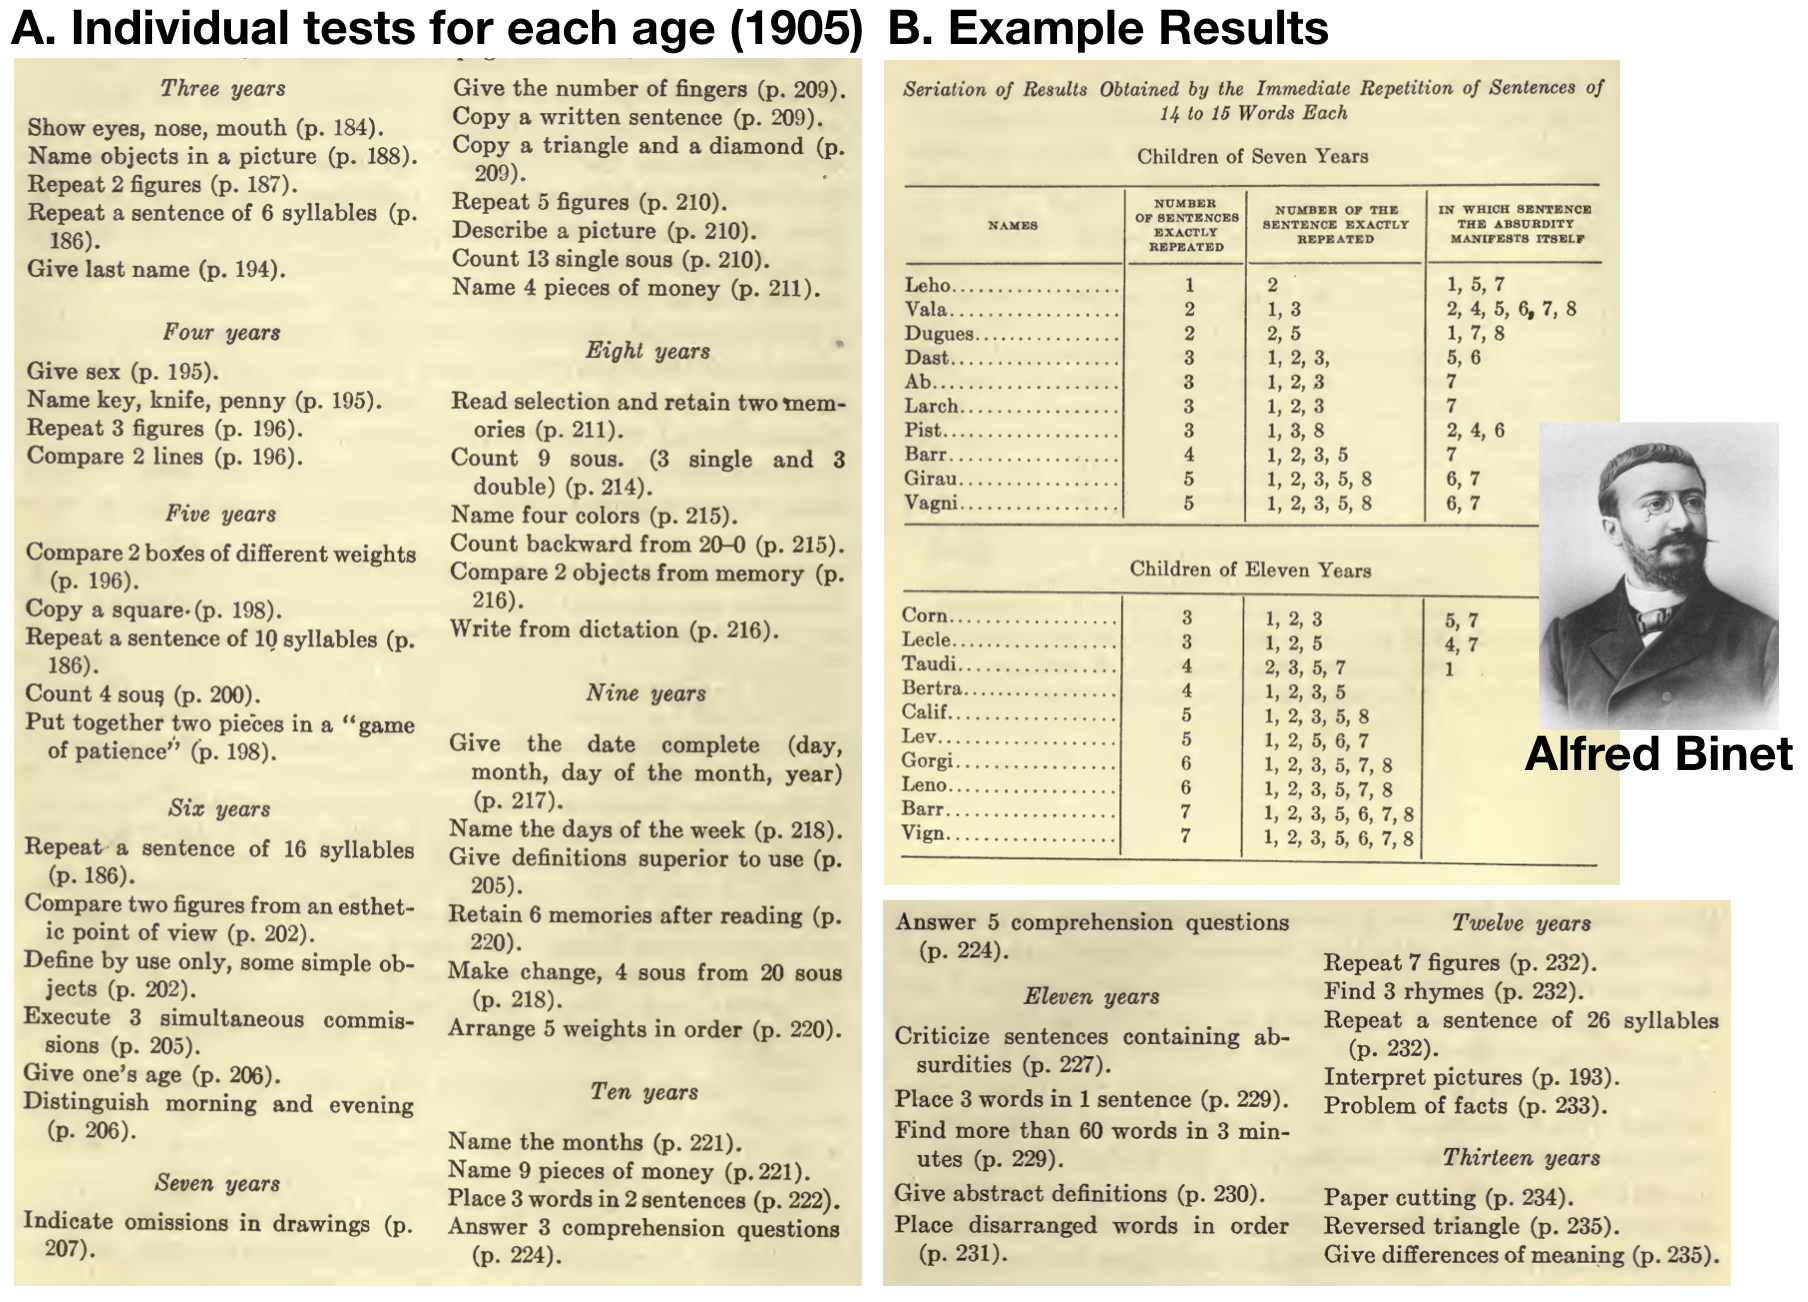
\includegraphics[width=1\linewidth]{imgs/Binet_1905}

To give an example of results, panel B shows performance from seven and eleven year old children on the task, ``immediate repetition of sentences of 14 to 15 words each''. In this task, a sentence was read aloud to a child, and the child had to repeat back the sentence exactly as many times as they could. Multiple measures of performance were taken, including total number of sentences repeated, and notes about ``absurdities'', occurring when the child repeated something that was determined by the examiner to be absurd. There are two important features of the results that were common to all of the tests, and that were fundamental to Binet's method. First, there were clear differences in task performance between children of different ages. For example, children at age seven year recited fewer sentences than children at ege eleven. To my eye, the average seven year old in the table (in the middle of the group) repeated about 3 sentences; whereas, the average eleven year old repeated about 5 sentences. Second, there were individual differences within children of the same age. Some children at age seven recited one or two sentences and other recited up to 4 or 5 sentences.

\hypertarget{quantifying-mental-ability-with-age}{%
\subsection{Quantifying mental ability with Age}\label{quantifying-mental-ability-with-age}}

Although Binet recognized that human intelligence was a large multi-dimensional concept, he nevertheless sought methods to quantify intelligence in simple ways, like using a ruler to measure length. Objects have different lengths that can be precisely measured with a ruler. Binet wanted a test that used numbers in a similar way for intelligence: larger numbers would indicate more intelligence and smaller numbers would indicate less.

One of Binet's problems was that he had many different varieties of tests, all which gave multiple measures of performance. He wanted to mash together the test results to a single dimension of numbers that would be simple, just like a ruler. Binet chose age in years. Age was simple like a ruler, going up in increments of one year at a time. Children also developed physically and mentally as they grew into adults. Binet's basic theoretical assumption was that, on average, children's mental abilities steadily increased ever year until they became adults. Thus, children at age seven would have more general intelligence than at age five, and eleven year olds would have more intelligence than ten year olds.

At the end of the day, Binet would invent a relative scale of measurement to capture what he claimed was human intelligence. The scale was relative to the average age of children, an intuitive number. Adults and children alike could be measured, and the test would return a number in years. A precocious seven year old might have a mental age of eleven, or an adult could be shown to have the mental abilities of a three year old.

\hypertarget{comparison-to-norms}{%
\subsection{Comparison to Norms}\label{comparison-to-norms}}

Binet was well aware that none of his specific tests measured anything as complicated as intelligence. He wrote, ``One test signifies nothing, let us emphatically repeat, but five or six tests signify
something. And that is so true that one might almost say, `It matters very little what the tests are so long as they are numerous.'.''\footnote{\protect\hyperlink{ref-binetNewInvestigationsMeasure1911}{Binet, A., \& Simon, T. (1911). New investigations upon the measure of the intellectual level among school children. \emph{L'Année Psychologique}, 145--201. \url{https://doi.org/c4b7b9}}.} What mattered more than the individual tests was Binet's innovation to compare test results from one individual to a larger group of individuals.

Binet employed the concept of average children, and assumed that every year, on average, children made gains in intelligence. He needed real-world estimates of his theoretical average children. To create the estimates he simply measured hundreds of children of different ages on his tests. For example, he gave many three year olds his tests and recorded how they performed. In this way, Binet obtained norms or standards that could be used for comparison. For example, the data on three year olds would show a spread of results. Some three year olds received lower scores, some were in the middle, and some received higher scores on the tests. This spread of results then becomes an empirical standard representing three year mental abilities. A parent could have their three year old measured on the tests, and Binet could tell the parent how their child performed relative to the other three year olds he had measured. Or, if a child was tested and scored as having the mental abilities of a seven year old, this would roughly mean that the child performed similarly to the seven year olds that Binet had measured while he was developing his scale.

Basing the measurement of mental abilities on a relative comparison to empirical norms is still very common in modern aptitude testing (e.g., the SAT, ACT, GRE, etc.), and otherwise known as standardized testing. One intriguing feature of the method is that the norms (e.g., what it means to be an average three year old, or four year old on the test) adjust themselves over time as more measurements are taken. For example, when Binet published his tests, he had only taken a limited number of measurements from three year olds, and these measurements served as the norms for three year olds. However, the norms for three year olds would update themselves as more three year olds were measured in the future.

\hypertarget{computing-intelligence-scores}{%
\subsection{Computing intelligence scores}\label{computing-intelligence-scores}}

In 1905, Binet had an unruly number of tests, well over 50; and, part of the testing process was to measure individual children on as many of the tests as possible. How did Binet take performance measurements from all of the tests to arrive at a single value in years that would quantify mental ability? Another way to state this question is to ask, how did Binet calculate average performance for the children in each age group, and how were the results from new children compared to the results from the existing children in Binet's database?

The answers are that Binet imposed rules for classification, and these rules determined how performance from individual tests was converted into an age in years. Binet experimented with different classification rules.

A potential rule was, ``A subject has the intellectual development of the highest age at which he passes all the tests, with the allowance of one failure in the tests for that age. Thus young Ernest has passed all the tests at nine years, except one; he has also passed all the tests at ten years except one; therefore we attribute to him the mental level of ten years.''\footnote{\protect\hyperlink{ref-binetDevelopmentIntelligenceChild1908}{Binet \& Simon, 1908}.}

By 1911, Binet settled on a more nuanced point system:

``Here is the rule to follow: take for point of departure, the age at which all the tests are passed; and beyond this age, count as many fifths of a year as there are tests passed. Example: a child of eight years passes all the tests of six years, 2 of seven years, 3 of eight years, 2 of nine years, 1 of ten years; he has therefore the level of six years plus the benefit of eight tests or eight-fifths years, or a year and three-fifths, equaling a level of seven years and three-fifths, or more simply 7.6. This calculation permits the appreciation of the intellectual level by means of a fraction. But it must be well understood that this fraction is so delicate an appreciation, that it does not merit absolute confidence, because it varies appreciably from one examination to another.''\footnote{\protect\hyperlink{ref-binetNewInvestigationsMeasure1911}{Binet \& Simon, 1911}.}

\hypertarget{binets-use-cases}{%
\subsection{Binet's use cases}\label{binets-use-cases}}

Binet achieved a method that would be used throughout the world to measure mental abilities. There are some strikingly simple properties of the test that make the method very seductive. The big idea was to create a large database of how children of various ages perform mental tasks, and then compare new people, measured on the same tasks, to the database. This would yield a ``mental age'', a simple number that represented mental abilities relative to a large and growing database.

One of Binet's use cases was to guard against bias when making decisions about child-welfare. Teachers might send children away to institutions just because they were unruly, and without an objective test of mental ability, the teacher could claim the unruly students were mentally unfit for school. Or, some children may have already been unjustly institutionalized, and without any objective way to show these children belong in a regular school, they would be forced to stay in the institution. Indeed, a major part of Binet's early demonstrations involved testing institutionalized children.\footnote{\protect\hyperlink{ref-binetNecessityEstablishingScientific1905}{Binet \& Simon, 1905c}.} On the one hand, he used these results to further validate his tests, because he was able to show that institutionalized children had lower ``mental ages'', when compared to non-institutionalized children. Thus, low scores on his tests could be used to justify institutionalizing children. On the other hand, Binet also found cases where institutionalized children were shown to be of ``normal'' intelligence relative to their non-institutionalized peers. Thus, scores on the tests could potentially be used to improve unjust treatment of children.

\hypertarget{meaning-of-the-measure}{%
\subsection{Meaning of the measure}\label{meaning-of-the-measure}}

We have just reviewed one of the first so-called ``intelligence'' tests developed by psychologists. However, up to this point we have mostly avoided giving a definition to the word intelligence. So, what is a definition of the word intelligence? And, does the Binet-Simon test actually measure intelligence according to that definition? If not, what does it measure?

\textbf{Operational definitions} are a research tool commonly used in psychology that will help us evaluate these issues. Operational definitions are used by individual researchers to specify the meaning of their own terms. For example, Binet could employ an operational definition of intelligence in terms of his own test. Here, the word intelligence would cease to have any common everyday meaning, and would only be used as a shorthand term to refer to patterns of performance on the test. And of course, just calling a test an ``intelligence'' test, doesn't mean that it measures the everyday meaning of intelligence. Clear operational definitions can benefit research because they allow researchers to communicate effectively, with clarity, and with terms that are limited to the context of the research. Operational definitions can also cause confusion, especially when researchers choose terms that already have well-established meaning in everyday usage. For example, using ``intelligence'' as a name for a test could easily confuse people who might assume the name was actually meaningful with respect to the everyday concept of intelligence.

Considering how operational definitions work, I can not give a clear answer about whether or not Binet's test actually measures intelligence. There are two problems. First, not everyone agrees on what intelligence is in the first place. Second, without an agreed upon definition, it is difficult to justify why each component of Binet's test actually measures some component of intelligence in a meaningful way.

Wikipedia gives the following definition of \href{https://en.wikipedia.org/wiki/Intelligence}{intelligence}:

``Intelligence has been defined in many ways: the capacity for logic, understanding, self-awareness, learning, emotional knowledge, reasoning, planning, creativity, critical thinking, and problem-solving. More generally, it can be described as the ability to perceive or infer information, and to retain it as knowledge to be applied towards adaptive behaviors within an environment or context.''

From my perspective, the meaning of intelligence is large, varied, and has different meanings for different people, just like the word cognition. As a result, it is difficult for any test to claim that it measures something as diffuse as intelligence. An analogy might be to music. Imagine someone claiming they had a music test that measured whether a given recording had more or less music, like a person could be claimed to have more or less intelligence. Music is so highly diverse that it would be ridiculous (in my opinion) to try to measure all of music on a single scale with a ``music test''. Plus, who get's to define what music get's counted as music? The surrounding issues that you might imagine would emerge from debates about a fictional music test, also surround debates about what intelligence tests mean.

Although I won't say I know what intelligence means, and I won't claim that the Binet-Simon test measures intelligence, I will claim that the Binet-Simon test can be inspected, and it is possible to assess the meaning of the measurement based on the procedures of testing that Binet described. For example, Binet used a process of trial-and-error to create mini-tests of different abilities that were age-appropriate. Specifically, Binet arranged the tests such that most children of a given age were able to complete the tests assigned to their own age group, and complete the tests assigned to younger age groups, but not complete tests assigned to older age groups. Also, Binet chose tests that produced variation within an age group--some children of the same age would do better or worse on the same test. Binet measured many children of all age groups on the tests. Then he proposed to compare new children, measured on the same tests, to his growing database.

So what does the Binet-Simon test measure? It measures how a child's performance on Binet's chosen mini-tests, compares to performance on the same mini-tests by groups of children of different ages. This is not a straightforward measure like a ruler, where one inch on the ruler, is one inch in the world. Although the Binet-Simon test produces a number in years, that refers to ``mental age''; the number is deceiving because it depends on many components. The components include the actual mini-tests that Binet chose, the children that Binet tested to form the empirical comparison group, and the classification rules that Binet used to assign years to children based on their test performance. Changes to any or all of these many components would change how a child would be scored, and what the score would actually mean.

\hypertarget{mental-testing-and-eugenics-in-america}{%
\section{Mental testing and eugenics in America}\label{mental-testing-and-eugenics-in-america}}

After the Binet-Simon test was translated to English, it was popularized in America as the Stanford-Binet test. Even though the test had numerous issues and was not actually a test of intelligence, it was nevertheless used in a widespread way throughout America. Many of the American psychologists who would use the new intelligence test were also advocates and members or leaders in eugenics societies. As a result, intelligence testing was used in America as a tool to further the cause of the eugenics movement.

\hypertarget{the-alpha-beta-test}{%
\subsection{The Alpha-Beta test}\label{the-alpha-beta-test}}

In 1917, the same year that America entered World War I, the APA appointed committees to study the situation and prepare for action,\footnote{\protect\hyperlink{ref-yerkesPsychologyRelationWar1918}{Yerkes, Robert M. (1918). Psychology in relation to the war. \emph{Psychological Review}, \emph{25}(2), 85--115. \url{https://doi.org/dhdj4j}}.} and the National Research Council created a Psychology Committee to examine similar issues.\footnote{\protect\hyperlink{ref-yoakumArmyMentalTests1920}{Yoakum, C. S., \& Yerkes, R. M. (1920). \emph{Army mental tests}. {H. Holt}}.} Many psychologist members of these committees were also members and proponents of eugenics, including: Robert Yerkes, Madison Bentley, Edward Thorndike, John B. Watson, Walter D. Scott, Robert Woodworth, and Carl Seashore (all of whom would take a turn as APA president).

War was a topic of considerable debate among eugenics societies,\footnote{\protect\hyperlink{ref-kuhlBettermentRaceRise2013}{Kühl, 2013}.} interesting in improving their race over generations. It was clear that many men would perish during war. On the one hand, according to the logic of eugenics, if ``low-quality'' men tended to perish, then war could be positive for eugenics, because those men would no longer be around to breed. On the other hand, ``high-quality'' men could be killed, and that would be a negative, because their genes would be lost as well. Additionally, a practical issue stood in the way, there was no process to measure the eugenic quality of soldiers, and then use that information to bias who is likely to live or die during war. Eugenicists were advocates of using intelligence tests on soldiers to help make personnel selection decisions, such as who gets to become an officer, and who gets to have a high probability of being killed by being sent to the front.

American Psychologist Robert Yerkes (APA president in 1917) overarching goal was establish a ``mental census'' of Americans, and then use that information to improve American society from a eugenics point of view. Although he urged testing of all Americans, Yerkes only carried out the largest mass testing on American men for the draft, administering the test to 1.75 million adults.\footnote{\protect\hyperlink{ref-yerkesEugenicBearingMeasurements1923}{Yerkes, Robert M. (1923). Eugenic {Bearing} of {Measurements} of {Intelligence} in the {United States Army}. \emph{The Eugenics Review}, \emph{14}(4), 225--245}.} There were two versions of the test (inspired along the lines of the Stanford-Binet test). The ``alpha'' test was created for soldiers who could read, and the ``beta'' test was created for soldiers who could not.

In his 1923 report, ``Eugenic Bearing of Measurements of Intelligence in the United States Army.'', Yerkes describes methods and results from the testing efforts, and lists the five main reasons to conduct such widespread testing:

''
(a). In the discovery of men whose superior ability recommends their advancement.
(b) In the prompt segregation in the Development Battalions of intellectually inferior men whose inaptitude would retard the training of the unit.
(c) In building organizations of equal or appropriate strength.
(d) In selecting suitable men for various army occupations or for special
training in the technical schools.
(e) In eliminating the feeble-minded.
''

\hypertarget{scientific-racism}{%
\subsection{Scientific Racism}\label{scientific-racism}}

Eugenics ideology typically included racist beliefs about the superior or inferior eugenic qualities of different ethnic groups.\footnote{\protect\hyperlink{ref-turdaRaceScienceEugenics2010}{Turda, M. (2010). Race, science, and eugenics in the twentieth century. \emph{The Oxford Handbook of the History of Eugenics}, 62--79}.} The Alpha-beta tests of 1.75 million American men also yielded results that fit existing eugenic ideology about inherent differences in intelligence between ethnic groups. For example, psychologist Carl Brigham, wrote an entire book analyzing the results of the Alpha-Beta tests.\footnote{\protect\hyperlink{ref-brighamStudyAmericanIntelligence1922}{Brigham, C. C. (1922). \emph{A study of {American} intelligence}. {Princeton: Princeton University Press; London: Oxford University Press \ldots{}}}.} He concluded that white Americans had superior intelligence to black Americans and immigrants. He also created dire warnings about the future of America, suggesting that American intelligence was rapidly declining. He warned that although American deterioration was imminent, it could be prevented through public action and laws. For example, eugenically inferior immigrants could be kept out of the country. And, increased segregation of whites and blacks, along with laws against intermarriage could prevent further mixing of the races.

As we discussed earlier, it is not entirely clear what these so-called intelligence tests measure, or what intelligence itself actually refers to. Nevertheless, proponents of eugenics were quick to claim that results from the tests really did legitimately measure supposedly intrinsic and genetically inherited qualities of humans that made some superior and others inferior. Alternative interpretations, such as the tests measured culturally acquired aptitudes, took additional time to be seriously considered. Unfortunately, racist motivations would continue to daunt intelligence testing in America, and an extended history is beyond the current scope of this chapter. Before, we conclude this chapter and examine future developments in the cognitive sciences, I cover two more historical examples related to intelligence testing and American Society.

\hypertarget{mental-health}{%
\subsection{Mental health}\label{mental-health}}

The eugenics movement deeply impacted public policy and stigma around mental health. We already mentioned that American eugenics proponents successfully petitioned for laws to legalize forcible sterilization of people deemed to be ``feeble-minded''. The invention of intelligence tests was heralded as a new scientific tool that aid in the identification of ``feeble-minded'' people, so that they could be segregated and/or sterilized. Psychologist Henry Goddard provides a case example of connecting intelligence testing to the eugenics agenda for treating mental health issues.

Goddard was Director of Research at the Vineland Training School for Feeble-Minded Girls and Boys in Vineland, New Jersey; and had published an English translation of Binet's work in 1916.\footnote{\protect\hyperlink{ref-kiteDevelopmentIntelligenceChildren1916}{Kite, 1916}.} Robert Yerkes visited Goddard and used his facilities at Vineland, during the development of the Alpha-Beta test. Goddard was heavily involved in eugenics, and one illustrative example is from his 1927 article, ``Who is a Moron?''\footnote{\protect\hyperlink{ref-goddardWhoMoron1927}{Goddard, H. H. (1927). Who is a moron? \emph{The Scientific Monthly}, \emph{24}(1), 41--46}.}

Goddard describes new terms for categorizing levels of ``feeble-mindedness'' based on intelligence tests. For example, ``idiots'' had the mental age of two-year old children, ``imbeciles'' had the intelligence of three to seven year olds. Goddard invented the term ``moron'' to describe people with the same supposed intelligence as eight to twelve year olds. The rest of the article describes eugenic ideology in the form of panic about how society is in danger unless it acts to solve the moron problem. The moron's were a problem because they appeared normal, and might only be identified with an intelligence test. As a result, hidden morons passing as normal people were running amok in society, and they also had many children, so they were potentially deteriorating the gene-pool by breeding. He considered extreme eugenic solutions, and wrote, ``perhaps our ideal should be to eventually eliminate all the lower grades of intelligence and have no one who is not above the twelve-year intelligence level'', but he also cautioned that eliminating half of society would be impossible and even undesirable. Instead, Goddard proposed that moron's could be cured through education, and become very useful to society as workers who would very happily do the jobs they were trained to do.

The overarching issues in mental health were very similar to what happened in the military. Intelligence tests were being forwarded as legitimate scientific measures of human quality that should be used to make decisions about the welfare of American citizens and their position in society.

\hypertarget{education-and-the-black-psychologists}{%
\subsection{Education and The Black Psychologists}\label{education-and-the-black-psychologists}}

As a final example, the methods involved in intelligence testing became widespread in education in the form of standardized testing. Similar to previous examples, proponents of eugenics were involved in these efforts. For example, the SAT was created by Carl Brigham, shortly after he published his book on ``A study of American Intelligence.''\footnote{\protect\hyperlink{ref-brighamStudyAmericanIntelligence1922}{Brigham, 1922}.} The eugenical ideals were that tests could be used to sort children in terms of their quality, and then give more resources to the education of superior children, and fewer resources to the education of inferior children.

Testing of american children showed achievement gaps between different ethnic groups. And, to fast forward into the 1960s, there was growing concern among Black Psychologists (only 1\% of a primarily white discipline at the time) that educational testing and decision-making policy was harming outcomes for Black children. In 1968, the \href{https://abpsi.org}{Association of Black Psychologists} (ABPsi) was formed as a national organization during the San Francisco meeting of the American Psychological Association (APA).\footnote{For a more complete history see, \protect\hyperlink{ref-williamsHistoryAssociationBlack1974}{Williams, R. (1974). A {History} of the {Association} of {Black Psychologists}: {Early Formation} and {Development}. \emph{Journal of Black Psychology}, \emph{1}(1), 9--24. \url{https://doi.org/gg3hq4}}.} The ABPsi was formed both to address needs within the small community of Black Psychologists that were not being met by the APA, and to petition the APA to address many broader concerns. For example, the ABPsi adopted the following statement on testing:

``The Association of Black Psychologists fully supports those parents who have chosen to defend their rights by refusing to allow their children and themselves to be subjected to achievement, intelligence, aptitude and performance tests, which have been and are being used to:

\begin{enumerate}
\def\labelenumi{\arabic{enumi}.}
\tightlist
\item
  Label black children as uneducable;
\item
  Place black children in special classes;
\item
  Potentiate inferior education; .
\item
  Assign black children to lower educational tracks than whites:
\item
  Deny black children higher educational opportunities; and
\item
  Destroy positive intellectual growth and development of black children.''
\end{enumerate}

The ABPsi's calls for a moratorium on testing\footnote{\protect\hyperlink{ref-gravesMoratoriumAfricanAmerican2011}{Graves, S., \& Mitchell, A. (2011). Is the {Moratorium Over}? {African American Psychology Professionals}' {Views} on {Intelligence Testing} in {Response} to {Changes} to {Federal Policy}. \emph{Journal of Black Psychology}, \emph{37}(4), 407--425. \url{https://doi.org/d56z38}}; see also, \protect\hyperlink{ref-williamsWhatHappenedABPsi1978}{Williams, R. L., \& Mitchell, H. (1978). What {Happened} to {ABPsi}'s {Moratorium} on {Testing}: {A} 1968 to 1977 {Reminder}. \emph{Journal of Black Psychology}, \emph{4}(1-2), 25--42. \url{https://doi.org/gg6btt}}.} in 1969 were not supported by the APA , whose membership also had financial interests in the large educational testing industry. Although there were efforts to maintain a relationship with the APA, the ABPsi formally became a distinct professional organization and has been publishing it's own journal since 1974. They have also been on the forefront of modern research on the impact and legacy of eugenics and racism in Psychology. Finally, although testing is still widespread in America, a moratorium on intelligence testing of Black children was accomplished in 1979 through advocacy of Black Psychologists in California,\footnote{\protect\hyperlink{ref-frisbySciencePoliticsBest2016}{Frisby, C. L., \& Henry, B. (2016). Science, {Politics}, and {Best Practice}: 35 {Years After Larry P}. \emph{Contemporary School Psychology}, \emph{20}(1), 46--62. \url{https://doi.org/gkzfj6}}.} where the practice remains illegal today.

\hypertarget{cognition-testing-abilities-vs.-testing-theories}{%
\section{Cognition: Testing abilities vs.~testing theories}\label{cognition-testing-abilities-vs.-testing-theories}}

This textbook is aimed at providing an overview of research into cognition. One piece of that history involves psychologists who were advocates of the eugenics movement, who created tests of cognitive abilities with the purpose of applying those tests on society to further the aims of the eugenics movement. The role of eugenics in motivating the need to create tests of cognitive ability, and in spreading the use of those tests across society is not commonly discussed in introductory textbooks. However, the historical context raises important questions about how the enterprise of scientific research contributes to societies that fund it, and we should be mindful of these issues as we move onto other topics in cognition. For example, it is clear that psychologists researching human cognition can produce tools of questionable merit that become widely adopted in society, and that continue to have positive and negative outcomes for different groups of people in society.

The next chapter begins to transition back to more conventional areas in cognitive psychology, like the domains of learning and memory. We will continue to see many more examples of cognitive tasks that are very similar, if not essentially the same, as the mini-tests used as part of intelligence scales. However, rather than testing for the purpose of measuring and classifying a person, we will discuss examples where cognitive tasks are used to test theories and claims about how cognition works.

\hypertarget{associations}{%
\chapter{Associations}\label{associations}}

\begin{tabular}{r|l|l}
\hline
Word Count & Reading Time & Last Compiled\\
\hline
7653 & 38.3 minutes & 2021-09-21 19:59:30 GMT\\
\hline
\end{tabular}

\hypertarget{chapter-overview-4}{%
\section{Chapter overview}\label{chapter-overview-4}}

The previous chapter covered research on cognitive abilities spanning roughly from the 1860s to the 1960s from the perspective of individual differences psychology. For example, in addition to developing mental tests, Alfred Binet wrote more broadly about his school of ``Individual Psychology,''\footnote{\protect\hyperlink{ref-nicolasProgramIndividualPsychology2014}{Nicolas, Coubart, \& Lubart, 2014}.} that was aimed at using measurements of variation in human attributes to make society more efficient. Individual differences was not the only approach to cognitive abilities. Instead, the methods of experimental psychology were also used to ask and answer questions about cognitive abilities. Experimental psychologists also developed tests, but they more often took the form of experimental manipulations. And, the results of the experiments were used to evaluate theories about how cognitive processes work. This chapter will focus on associationism and early empirical work on associative learning processes in humans and non-human animals.

\hypertarget{evolving-ideas-on-cognition}{%
\section{Evolving ideas on cognition}\label{evolving-ideas-on-cognition}}

There is a long history of ideas about cognition that predate and feed into psychological approaches to cognition, and covering all of them is beyond the scope of this chapter. However, if we zoom in on early experimental research between the 1890s to 1920s, we can refer to some of the intellectual history and see how it informed and guided cognition research at the time. Some of the really big claims and themes about cognition that appear in the introductions of early research manuscripts remain relevant today.

We are about to visit the laboratories of \href{https://en.wikipedia.org/wiki/Edward_Thorndike}{Edward Thorndike} (1874-1949) and \href{https://en.wikipedia.org/wiki/Ivan_Pavlov}{Ivan Pavlov} (1849-1936). Thorndike was in America and Pavlov was in Russia, and both were independently conducting novel experiments to test theories and claims about cognition in animals. Before we review their experiments and findings, let's first consider the background claims and ideas they intended to put to the test.

\hypertarget{humans-and-animals}{%
\subsection{Humans and animals}\label{humans-and-animals}}

So far we have discussed cognition in terms of human animals. But, there are so many other animals of all shapes and sizes, what about them? Prior to Thorndike and Pavlov, there wasn't too much experimental research on cognition in the animal kingdom, but since then whole fields of animal and comparative cognition have been developed. Although this textbook will focus more on human cognition, I will attempt to integrate animal cognition as much as possible. And, rather than using ``human-animal'', and ``non-human animal'', I will refer to human and/or animal cognition throughout the book as a shorter way to identify the subjects of the research. Last, discussions about which words to use to refer to humans and animals point to background ideas motivating Thorndike and Pavlov's work.

Just like there is a long human history of ideas about the mind, there is long history of ideas about animals, animal minds, and the human-animal relationship. \href{https://en.wikipedia.org/wiki/Anthropocentrism}{Anthropocentrism} is a variety of beliefs and traditions that center on humans as the most important species. For example, in early Judaic and Christian writings, a supreme supernatural being created humans in their image and set humans on a higher level than other animals. These ideas both distinguish humans from animals (as being different kinds of entities), and place humans in a hierarchy of quality above other animals. Judeo-Christian concepts predate psychology by thousands of years, and even though psychology as a natural science proceeded to construct different views on humans and animals, related hierarchical notions remain deeply ingrained. For example, ``higher-order'' cognition is often reserved for cognitive abilities argued to be special to humans, like inferential reasoning. And, ``lower-order'' cognition is often reserved for basic cognitive abilities that are common among animals. It's not clear to me that these hierarchies are very useful.

\href{https://en.wikipedia.org/wiki/Animism}{Animism} is another varied set of beliefs ascribing spiritual essences to things, including animals. Many fables, folklore, and religious texts have animal characters imbued with cognitive abilities and other powers. Relatedly, the idea that animals can be understood as if they were humans is also criticized as an inaccurate form of anthropomorphism.

Mystic ideas about humans and animals can be viewed as claims about cognition. One claim is about whether or not human cognition can be explained at all. The idea that people were created in the image of a fundamentally unexplainable supernatural being, suggests that the supernatural parts of people are inherently unexplainable. Another claim is about kinds of cognitive abilities. For example, the idea that animals possess vital spiritual essences like humans, could suggest that mental abilities of some animals are similar to people. Experimental Psychology arose out of the scientific tradition to put claims to the test by collecting evidence bearing on the claims.

\hypertarget{philosophy}{%
\subsection{Philosophy}\label{philosophy}}

The experiments of Thorndike and Pavlov are also set in a background of philosophy, especially debates in \href{https://en.wikipedia.org/wiki/Epistemology}{epistimology} between \href{https://plato.stanford.edu/entries/rationalism-empiricism/}{rationalist and empiricist views of knowledge}.

\href{https://en.wikipedia.org/wiki/Rationalism}{Rationalism} involved views that some knowledge was innate and could exist separately from experience and information gained through sense organs. Furthermore, ultimate truths about reality were argued to depend on logic and reason. If the universe was a fundamentally logical place, then the process of accurate reasoning alone would be enough to deduce the ultimate truths.

\href{https://en.wikipedia.org/wiki/Empiricism}{Empiricism} additionally emphasized a role for observation and evidence collection in knowledge creation. For example, human's were argued to acquire knowledge over the course of their experience of the world through their sense organs. Empiricism invited further questions about how people created knowledge from their sensory experience, which clearly connected to questions of interest for early experimental psychologists.

The \href{https://en.wikipedia.org/wiki/Associationism\#Associationist_School}{Associationist School} included empiricist philosophers who speculated further on the nature of mental processes that produced knowledge from experience. In 1689, John Locke wrote, ``An essay concerning human understanding'', and argued against the rationalist/nativist idea that people were born only with innate knowledge about the world. Instead, Locke advocated that people acquired knowledge by learning about the world through their experiences. In 1739, David Hume elaborated on the nature of the learning process and suggested a role for associations in, ``Treatise on Human Nature'', that ``when the mind, therefore, passes from the idea or impression of one object to the idea or belief of another, it is not determined by reason, but by certain principles, which associate together the ideas of these objects, and unite them in the imagination.''. Hume suggests broadly that acts of cognition involve a process of association that works according to ``certain principles''. What the principles are, and how they work, is still a primary focus of the modern cognitive sciences.

Principles of association included roles for contiguity, similarity, frequency, and recency to shape the formation of new associations. \emph{The principle of contiguity} states that strength of association depends on the proximity of events in space and time. Events that are closer to each other are associated more strongly. \emph{The principle of similarity} states that more similar events will develop stronger associations than less similar events. \emph{The principle of frequency} is that events that co-occur more frequently will be associated more strongly than less frequent events. \emph{The recency principle} suggests stronger associations for recent events than more remote events. In general, these philosophical principles of association have held up quite well and are often components of modern theories.

\hypertarget{natural-science}{%
\subsection{Natural Science}\label{natural-science}}

There is also lesser known work from Robert Hooke (1635-1703), a natural scientist, that went much further than Hume's ``certain principles''. Robert Hooke, coined the word cell, and was the first person to observe a micro-organism under a microscope. In 1705, Hooke's posthumous works were published, and they contained his model of how human memory could operate as a physical system.\footnote{\protect\hyperlink{ref-hookePosthumousWorksRobert1705}{Hooke, R. (1705). \emph{The posthumous works of {Robert Hooke}: {With} a new introduction by {Richard S}. {Westfall}}. {New York: Johnson Reprint Corp}}.} The model was not entirely physical, because it allowed some role for ``immaterial'' forces; and, it was largely forgotten until fairly recently.\footnote{\protect\hyperlink{ref-hintzmanRobertHookeModel2003}{Hintzman, D. L. (2003). Robert {Hooke}'s model of memory. \emph{Psychonomic Bulletin \& Review}, \emph{10}(1), 3--14. \url{https://doi.org/fd9wxx}}.} However, despite not having a major historical impact, Hooke's model was a clear attempt to move toward well-specified mechanistic explanations of cognition \footnote{we will examine several models of human memory in greater detail in the upcoming chapters on memory}.

\hypertarget{evolution}{%
\subsection{Evolution}\label{evolution}}

A last backdrop to the upcoming works of Thorndike and Pavlov was Darwin's theory of evolution. Darwin's theory connected all life on earth and explained the origins of species in terms of natural selection processes. The critical ingredients for organisms to evolve over generations include 1) the ability to reproduce, 2) random mutations that produce heritable variations in the traits and behavior of the organism, and 3) environmental selection pressures. Organisms with advantages for survival in their particular environments would tend to pass on those traits to their offspring. Other organisms that were more likely to succumb to their environments, would be less likely to have offspring and pass on their heritable traits. In this way, organisms would slowly drift and change across generations based on whichever random mutations tended to facilitate those organisms reproducing and mutating over generations in their given environments.

Different from anthropocentric views, the theory of evolution clearly sets humans and animals in the very same explanatory ballpark. People are a species of animals with an evolutionary family tree, where every person is descended from their parents. Other animals have their own evolutionary family trees and lineages of descendants. Furthermore, if one went far enough back in the family tree, all animals could be descended from common ancestors.

Considering evolutionary theory, there is every good reason to consider cognition as a topic for humans and animals. First, humans are animals; so by definition human cognition is a specific case of animal cognition. Second, there are a wide variety of animals that range in their physical size and capabilities, and it seems implausible that an evolutionary process would only bestow cognitive processes onto humans and no other animals. Instead, evolutionary theory implies that cognitive processes among animals also evolved over time. This could imply that the field of cognition is as large and diverse as all the ways that cognitive processes might have evolved differently across species. At the same time, evolution is known to produce similar solutions across species (e.g., eyes), and it is plausible that animals share cognitive processes that work on the basis of similar principles.

So, the backdrop to Thorndike and Pavlov was western European cultural beliefs about humans and animals, western philosophical debates centering around psychological constructs like human knowledge, a desire to apply the rigors of natural science methodology to problems in psychology, a convincing theory of evolution suggesting that animals could be used as subjects to gain knowledge about evolutionary basic cognitive processes, and a wide open playing field where there was very little existing empirical work.

\hypertarget{associative-claims}{%
\subsection{Associative Claims}\label{associative-claims}}

If you took the position that cognition was a special ability that operated according to special rules that can never be known, it would not be possible to evaluate those claims with evidence. First, its not clear what ought to happen in any given situation if cognition is special and unexplained. Second, if any particular thing happened, it could be accounted for by saying that cognition is special like that.

Associationist claims are specific enough that they can be evaluated with evidence. As a result, it becomes possible to use the scientific method to assess claims about cognition. Let's identify a few really basic claims that could be evaluated.

\begin{enumerate}
\def\labelenumi{\arabic{enumi}.}
\tightlist
\item
  People have associations between concepts
\item
  New associations can be learned
\item
  Some associations are stronger than others
\end{enumerate}

First, could you think of examples from your experience that would provide evidence for these claims? Have you ever learned a new association between one thing and another? Are some ideas more strongly associated with others in your experience? I've learned many things that could involve associations. For example, I didn't know how to type on a computer keyboard when I was born, I learned how to do it. Now, I barely think about what my fingers are doing when I type because the words I'm thinking are strongly associated with the finger movements I need to make to type the sentence I want to write. It's easy to demonstrate for yourself that some associations are stronger than others. For example, think of a fruit that begins with the letter ``A''. How long did that take? Think of any word that has a letter A in the 5th position of the word? Did that take longer? The letter A seems to be more strongly associated with some words than others.

Although, you could come up with additional examples from your experience that would be consistent with the claims, consider the problem of creating a laboratory-based demonstration. One goal of a laboratory-based demonstration is to describe a method and controlled set of circumstances that other people could use to reproduce your demonstration and verify your results. The following are early laboratory demonstrations that were used to evaluate the associationist claims.

\hypertarget{cattells-associative-reaction-times}{%
\section{Cattell's Associative Reaction times}\label{cattells-associative-reaction-times}}

We met James McKeen Cattell in the last chapter, as he was an early proponent of mental ability testing before Binet. Cattell also used experimental psychology methods to ask gather evidence about associative processes in people.

\hypertarget{naming-times}{%
\subsection{Naming times}\label{naming-times}}

In one set of studies he measured how long it took people to see and name objects.\footnote{\protect\hyperlink{ref-cattellTIMETAKENCEREBRAL1886}{CATTELL, J. M. (1886). {THE TIME TAKEN UP BY CEREBRAL OPERATIONS}. \emph{Mind}, \emph{os-XI}(42), 220--242. \url{https://doi.org/c5z6fm}}; \protect\hyperlink{ref-cattellTimeItTakes1886}{Cattell, James McKeen. (1886). The time it takes to see and name objects. \emph{Mind}, \emph{11}(41), 63--65. \url{https://doi.org/b6fr5r}}.} The ability to identify an object by naming it out loud was presumed to involve an association between perceiving the object and the action needed to utter the object's name. One of Cattell's findings was that people take twice as long to read words that ``have no connexion'', compared to words that are in a sentence; and, twice as long to read letters that are not in order, compared to letters that are in words.

For example, Cattell's subjects were twice as fast to read a regular versus scrambled sentence \footnote{These are not original stimuli used by Cattell}

\begin{floatrightbox50}
\textbf{Try it yourself}

\emph{Read each of the words below as fast as you can.}

\begin{enumerate}
\def\labelenumi{\arabic{enumi}.}
\item
  \emph{Regular Sentence}: The candy at the store was red and very tasty
\item
  \emph{Scrambled Sentence}: very at red and The tasty the was store candy
\end{enumerate}

\emph{Were you slower to read the words in the scrambled sentence?}

\end{floatrightbox50}

Similarly, if the task was to read individual letters one a time, Cattell's subjects were twice as fast to read letters when they occurred in words compared to when they did not. This general finding was later re-discovered, and termed the word-superiority effect in 1969.\footnote{\protect\hyperlink{ref-reicherPerceptualRecognitionFunction1969}{Reicher, G. M. (1969). Perceptual recognition as a function of meaningfulness of stimulus material. \emph{Journal of Experimental Psychology}, \emph{81}(2), 275. \url{https://doi.org/dq8xp9}}.}

\begin{floatrightbox50}
\textbf{Try it yourself}

\emph{Read each of the} \textbf{letters} \emph{as fast as you can.}

\begin{enumerate}
\def\labelenumi{\arabic{enumi}.}
\item
  \emph{Letters in words}: very at red and The tasty the was store candy
\item
  \emph{Scrambled letters}: tyshe noact aer ead ta rrdth des etyv Twnasy
\end{enumerate}

\emph{Was it harder to read the scrambled letters?}

\end{floatrightbox50}

Let's relate Cattell's general findings to the associative claims that people have associations between concepts, they can learn new associations, and that some associations are stronger than others. The first two claims are consistent with reading ability in general, which involves learning connections between an arbitrary symbol system (e.g., alphabetic letters) and vocal outputs. Cattell's results are also consistent with the claim that some associations are stronger than others. For example, it appears that reading time does not just involve the time it takes to recognize and say a word or letter. If this was strictly the case, then people would take the same amount of time to read words and letter no matter if they occurred in sentences or words. Instead, people were faster to read words and letters when they appeared in familiar contexts, like sentences and words. This suggests that information from the surrounding context facilitates reading, possibly through some kind of association.

\hypertarget{association-reaction-times}{%
\subsection{Association reaction times}\label{association-reaction-times}}

In the following year, Cattell turned his reaction time methods more directly toward the problem of measuring associations, along with the amount of time taken by intervening cognitive processes involved in the associative process.\footnote{\protect\hyperlink{ref-cattellExperimentsAssociationIdeas1887}{Cattell, James McKeen. (1887). Experiments on the association of ideas. \emph{Mind}, \emph{12}(45), 68--74. \url{https://doi.org/d9bv2m}}.} In the introduction to this paper he wrote:

\begin{quote}
``{[}In previous work..{]} 0.4 seconds was needed to see and name a word. When the physiological factors and the time taken up in seeing the word were eliminated, it was found that about 0.1 seconds was spent in finding the name belonging to the printed symbol. The time was longer for letters, which we do not read as often as words, and still longer (about .25 sec) for colours and pictures. I called the time passing, while the motor expression was being found, a `Will-time'.''
\end{quote}

We will elaborate on reaction time methods in the next chapter. For now, it is worth pointing out two aspects of this measurement tool for understanding how cognitive processes might work. First, it is possible to measure reliable differences in reaction times when people complete particular tasks. For example, Cattell estimated that 400 milliseconds were needed to see and read a word, and that pictures took a little bit longer. Second, it is possible to speculate about the individual components of processing that account for the total reaction time. For example, Cattell divides up the reaction time for a word into physiological factors and time taken up be seeing the word, followed by the time taken to search and recall the name of the word, and finally the time taken to form the action to say the word.

In the remainder of the paper, Cattell gave subjects an association task that involved 1) receiving a cue/prompt, and 2) responding with a known association to the cue. For example, participants were shown a picture and asked to name in their first or second language. Cattell found faster picture naming in a first than second language, and argued that people had more practice naming objects in their first than second language. Another study simply measured the times associated remembering different kinds of facts given a cue. For example, the cue was a city, and subjects had to remember the country it was in. Or, the cue was a month, and subjects recalled what season it was in, or the preceding, or following month. Cattell reported average reaction times and showed consistent differences depending on the cue and associative response. Cattell speculated that different reaction times reflected corresponding differences in the mental operations needed to carry out each task.

\hypertarget{thorndikes-puzzle-boxes}{%
\section{Thorndike's puzzle boxes}\label{thorndikes-puzzle-boxes}}

\href{https://en.wikipedia.org/wiki/Edward_Thorndike}{Edward Thorndike} (1874-1949) was a student of Cattell who took some of the first experimental approaches to investigating associative processes in non-human animals \footnote{Thorndike also followed Cattell in becoming a strong proponent and public figure in the American eugenics movement}.

\begin{floatrightbox25}
\textbf{Edward Thorndike}

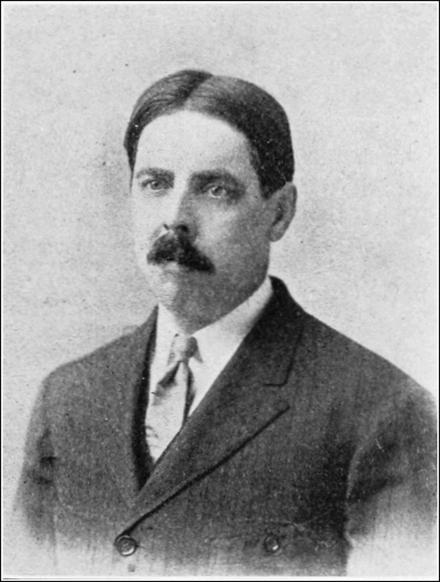
\includegraphics[width=1\linewidth]{imgs/Edward_thorndike}

\end{floatrightbox25}

Thorndike viewed previous claims about animal cognition as belonging to two wildly different camps, with almost no middle ground, or evidence to interrogate the claims. In one camp, animals might be near human, potentially being able to reason and form associations on par with people. In the other camp, animals might be simple reflex machines and nothing more.

Here are a few choice quotes from Thorndike's doctoral thesis\footnote{\protect\hyperlink{ref-thorndikeAnimalIntelligenceExperimental1898}{Thorndike, E. L. (1898). Animal intelligence: {An} experimental study of the associative processes in animals. \emph{The Psychological Review: Monograph Supplements}, \emph{2}(4), i--109. \url{https://doi.org/bk48z2}}.} that illustrate his thinking and approach to the study of animal intelligence.

\begin{quote}
``We do not know how delicate or how complex or how permanent are the possible associations of any given group of animals.''
\end{quote}

\begin{quote}
``We say that the kitten associates the sound''kitty kitty'' with the experience of nice milk to drink, which does very well for a common-sense answer. It also suffices as a rebuke to those who would have the kitten ratiocinate about the matter, but it fails to tell what real mental content is present. Does the kitten feel ``sound of call, memory-image of milk in a saucer in the kitchen, thought of running into the house, a feeling, finally, of `I will run in'?'' Does he perhaps feel only the sound of the bell and an impulse to run in, similar in quality to the impulses which make a tennis player run to and fro when playing? The word association may cover a multitude of essentially different processes, and when a writer attributes anything that an animal may do to association his statement has only the negative value of eliminating reasoning on the one hand and instinct on the other\ldots To give to the word a positive value and several definite possibilities of meaning is one aim of this investigation.''
\end{quote}

\begin{quote}
``Surely every one must agree that no man now has a right to advance theories about what is in animals' minds or to deny previous theories unless he supports his thesis by systematic and extended experiments. My own theories\ldots{} will doubtless be opposed by many. I sincerely hope they will, provided the denial is accompanied by actual experimental work. In fact I shall be tempted again and again in the course of this book to defend some theory, dubious enough to my own mind, in the hope of thereby inducing some one to oppose me and in opposing me to make the experiments I have myself had no opportunity to make yet.''
\end{quote}

To summarize these quotes, Thorndike was interested in settling debate and ideas about animal intelligence using laboratory techniques and the scientific method. This would involve creating reproducible situations in lab where animal behavior could be manipulated and observed under different experimental conditions. Thorndike argued that his methods would be produce evidence about claims of animal intelligence, and that his methods could be used by other researchers both to verify his findings and to test his theories and claims even further. Thorndike's method of assessing associations in animals involved puzzle boxes, or the modern equivalent of an \href{https://en.wikipedia.org/wiki/Escape_room}{escape rooms} for animals.

\hypertarget{thornikes-basic-methodology}{%
\subsection{Thornike's basic methodology}\label{thornikes-basic-methodology}}

Thorndike conducted multiple experiments on cats, dogs, and chicks. His experimental apparatus was in the form of a puzzle box, like the one depicted below:

\begin{floatright50}
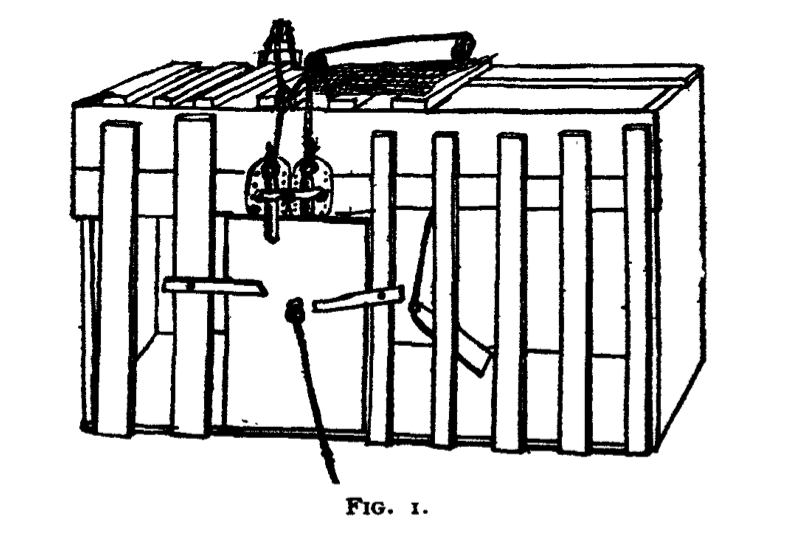
\includegraphics[width=1\linewidth]{imgs/Thorndike_puzzle_box_1898}

\end{floatright50}

Thorndike made several variations on his puzzle boxes, but they all had the same basic features in common. First, animals could be placed inside the box. Second, animals could escape from the box if they figure out the trick. For example, pulling a latch, or a hoop on a string would unlock a door allowing the animal to escape. Animals were typically deprived of food and made hungry before they were placed in the box. And, they were given a food reward after they escaped from the box. Animals were given many practice attempts to get out of the box, and Thorndike measured the amount of time to get out of the box for each attempt.

\hypertarget{putative-mental-components-of-association}{%
\subsection{Putative Mental Components of Association}\label{putative-mental-components-of-association}}

Thorndike's methods produced clear findings. His first main finding was that his animals could figure out the tricks, and they were able to escape from the box. His second main finding was that the animals got faster at escaping with practice. After making these demonstrations, Thorndike then considered possible explanations. How were the animals solving the problem? How were they getting faster? What kinds of associations were involved?

Thorndike's aim was to gain clarity on the kinds of associations that might be involved, and he speculated on logical stages and types of associations that his animals might have been learned. For example, he wrote:

\begin{quote}
There might be in an association, such as is formed after experience with one of our boxes, the following elements:
\end{quote}

\begin{enumerate}
\def\labelenumi{\arabic{enumi}.}
\tightlist
\item
  Sense-impression of the interior of the box, etc.
\item
  Discomfort and desire to get out.
\item
  Representation of oneself pulling the loop.
\item
  Fiat comparable to the human ``I'll do it.''
\item
  The impulse which actually does it.
\item
  Sense-impression of oneself pulling the loop, seeing one's paw in a certain place, feeling one's body in a certain way, etc.
\item
  Sense impression of going outside.
\item
  Sense impression of eating, and the included pleasure. Also between 1 and 4 we may have
\item
  Representations of one's experience in going out,
\item
  Of the taste of the food, etc.
\end{enumerate}

This list details a number of experiences and impulses that presumably occur from the time when an animal enters the box, to the time after it has escaped and is eating the food reward. The general associationist explanation would be that each of these components are associated with one another, possibly in a chain, such that triggering one of the elements would cause a chain reaction, and successively trigger the next associated element, thereby allowing the animal to proceed through the puzzle box and get the food reward.

\hypertarget{experimental-questions-about-associative-processes}{%
\subsection{Experimental questions about associative processes}\label{experimental-questions-about-associative-processes}}

Thorndike also went on to conduct experiments with his puzzle boxes to test ideas about animal learning. These experiments involved manipulations intended to modify some aspect of the learning process.

\hypertarget{imitation-learning}{%
\subsubsection{Imitation Learning}\label{imitation-learning}}

Thorndike found that cats, dogs, and chicks did not benefit from watching other animals solve the puzzle box. This didn't definitely rule out imitation as a possible source of knowledge, and it suggested to Thorndike that some elements of the associations needed to be experienced directly to be learned. Thorndike had plans to test whether an ape could learn to escape a box through imitation learning, but was unable to conduct the experiment because the monkey was not tame-able.

\hypertarget{mental-representation}{%
\subsubsection{Mental Representation}\label{mental-representation}}

As we will see throughout this textbook, theories of cognition often invoke the concept of mental representation. The previous chapter on mental imagery was an example of debates about the format of mental representations and whether they have analog-image like qualities (e.g., like sensory experiences), or are fundamentally very different, perhaps like abstract propositional knowledge. Thorndike was optimistic his methods could help settle questions of mental representation in animals. For example, do animals have internal images that are used in a network of associations? Thorndike proposed the following experiment:

\begin{quote}
``The only logical way to go at this question and settle it is, I think, to find some association the formation of which requires the presence of images, of ideas. You have to give an animal a chance to associate sense-impression A with sense-impression B and then to associate B with some act C so that the presence of B in the mind will lead to the performance of C. Presumably the representation of B, if present, will lead to C just as the sense-impression B did. Now, if the chance to associate B with A has been improved, you ought, when the animal is confronted with the sense-impression A, to get a revival of B and so the act C. Such a result would, if all chance to associate C with A had been eliminated, demonstrate the presence of representations and their associations.''
\end{quote}

\hypertarget{general-concept-formation}{%
\subsubsection{General concept formation}\label{general-concept-formation}}

Another topic in cognition that we devote a whole chapter to is categorization and concept formation. Thorndike attempted experiments to determine the ability of his animals to form general concepts about the puzzle boxes. Consider a kitten who has learned to escape from a puzzle box by pulling a loop on a string. Is the learning very specific or very general? It's possible that learning could be very, very specific (and we will see many examples in this textbook where learning very often is very specific). For example, the kitten may only escape from the specific puzzle box it had been trained on, and it would fail to easily learn other similar boxes, even those that contained loops in other locations about the box. Alternately, maybe the kitten learned general concept, something like, ``to escape the box, go around and find the loopy thing, and then tug it''. In this case, if the kitten learned a general concept, it might easily escape from similar boxes that involved pulling loops, even the loops were in novel locations in the box.

Thorndike tested these ideas in \textbf{transfer} experiments. Here, animals first learned to escape from a particular box, and then learned to escape from new boxes. The empirical question was whether learning to escape from the first box would help animals learn to escape from the next box. For example, if a kitten learned to pull a loop on the left side of the box to get out, would they quickly learn to escape out of a box with the loop on the right side? Thorndike found evidence of \textbf{positive transfer}, which means that the training experience conveyed a benefit on the transfer test. His animals learned to escape from a new puzzle box faster when it was similar to a puzzle box they had learned previously. Although the evidence of positive transfer could be consistent with a claim that his animals were learning a general concept about the puzzle box, Thorndike favored the view that animals were not learning general concepts, and instead were learning about specific details of the puzzle box that happened to transfer well to similar boxes. In other words, he attempted to example the phenomena of transfer without appealing to a complex explanation, like imbuing kittens with human-like general reasoning abilities.

\hypertarget{further-associative-questions}{%
\subsection{Further associative questions}\label{further-associative-questions}}

Thorndike created a laboratory method that produced reproducible patterns of evidence related to questions about animal cognition. There weren't many other researchers at that time applying methods of experimental psychology to animals, and Thorndike hoped his methods would be adopted by others for the purpose of challenging and extending his own work. In addition, Thorndike entertained questions about associations that ought to be studied in the future. Some of these questions included:

\begin{enumerate}
\def\labelenumi{\arabic{enumi}.}
\tightlist
\item
  Delicacy and permanence of associations: How fragile are some associations, how long do associations last after they have been formed?
\item
  Complexity of associations (Thorndike intended to rank intelligence of animals as a function of the complexity of associations they could acquire)
\item
  Number of associations: How many associations do different animals have?
\item
  Inhibition of instinct by habit: Can an animal learn to override an instinctual behavior through associative learning?
\item
  Role of attention: does the formation of an association depend on attending to sense-impressions?
\end{enumerate}

\hypertarget{pavlovs-classical-conditioning}{%
\section{Pavlov's Classical Conditioning}\label{pavlovs-classical-conditioning}}

Around the same time as Thorndike was conducting experiments to better understand associative processes in animals, Ivan Pavlov was conducting his own experiments on associative learning in animals using his own novel methods. Pavlov was in Russia and was not aware of Thorndike's work until much later. Pavlov's experiments were translated to English as a series of lecture in 1927.\footnote{\protect\hyperlink{ref-pavlovConditionedReflexesInvestigation1927}{Pavlov, I. P. (1927). \emph{Conditioned reflexes: {An} investigation of the physiological activity of the cerebral cortex} (A. G. V., Ed.). {London: Oxford University Press}. \url{http://books.google.com/books?hl=en\&lr=\&id=cknrYDqAClkC\&oi=fnd\&pg=PA1\&dq=pavlov\&ots=KAnkq8Z5Jb\&sig=9io8iEUzHMM3wDB0J7cMjT-bEcY}}.}

Thorndike approached his questions about animal learning from the perspective of Experimental Psychology, whereas Pavlov was skeptical of psychology as a natural science, and approached questions about animal learning from the perspective of a physiologist (or, a modern neuroscientist). Whereas Thorndike considered ``psychic'' phenomena such as mental images in his explanations of animal learning; Pavlov was more interested in measuring observable phenomena such as behavior, as well as physical substances, such as secretions, apparently produced by brain processes. Here are a few quotes from Pavlov:

\begin{quote}
``The cerebral hemispheres stand out as the crowning achievement in the nervouse development of the animal kingdom. These structures in the higher animals are of considerable dimensions and exceedingly complex, being made up in man of millions upon millions of cells--centres or foci of nercous activity-- varying in size, shape, and arrangement, and connected with each other by countless branchings from their individual processes. Such complexity of strucgture naturally suggests a like complexity of function, which in fact is obvious in the higher animal and in man. Consider the dog, which has been for so many countless ages the servant of man. Think how he may be trained to perform various duties, watching hunting, etc. We know that this complex behaviour of the animal, undoubtedly involving the highest nervous activity, is mainly associated with the cerebral hemispheres. If we remove the hemispheres in the dog,\footnote{\protect\hyperlink{ref-goltzHundOhneGrosshirn1892}{Goltz, F. (1892). Der hund ohne grosshirn ({The} dog without a cerebrum). \emph{Archiv Für Die Gesamte Physiologie Des Menschen Und Der Tiere}, \emph{51}(11), 570--614}.} the animal becomes not only incapable of performing these duties but also incapable even of looking after itself.''
\end{quote}

\begin{quote}
``In astounding contrast with the unbounded activity of the cerebral hemispheres stands the meagre content of present-day physiological knowledge concerning them. Up to the year 1870, in fact, there was no physiology of the hemispheres; they seemed to be out of reach of the physiologist''.
\end{quote}

Pavlov wrestled with whether or not psychology should be involved with attempts to explain brain functions. He thought that the psychological perspective was less-exact and prone to non-physical interpretations, where the brain was implicated in some kind of ``special psychical activity''. And, he suggested that, ``there is no need for the physiologist to have recourse to psychology'', and that ``investigations of the physiological activities of the hemispheres should lay a solid foundation for a future true science of psychology.''.

\hypertarget{descartes-reflex}{%
\subsection{Descartes' reflex}\label{descartes-reflex}}

\begin{floatrightbox25}
\textbf{Réne Descartes}

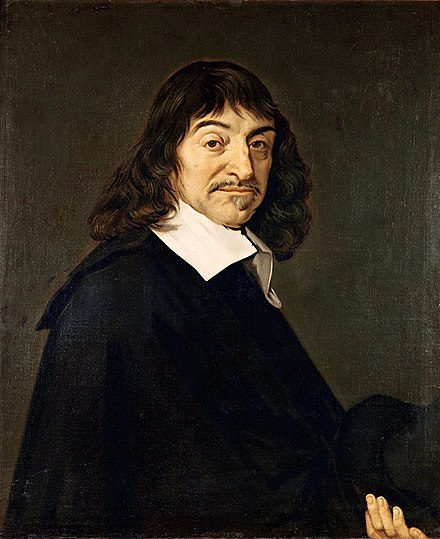
\includegraphics[width=1\linewidth]{imgs/Rene_Descartes}

\end{floatrightbox25}

Before describing his experiments, Pavlov connected his work to philosophical ideas about humans and animals popularized much earlier by \href{https://en.wikipedia.org/wiki/René_Descartes}{René Descartes} (1596-1650). Descartes was a rationalist philosopher who advanced a dualist perspective of the mind. According to Descartes, humans had a physical body that operated like a physical machine that obeyed the laws and principles of physical machines. But, humans also had a soul that did not operate according to physical laws. The human soul was the mysterious quality that set humans apart from animals which were viewed as less than human. Animals had physical bodies, but no soul. Although Descartes advocated for dualism, his ideas about how human and animal bodies behaved like complicated machines were inspirational to physiologists,\footnote{\protect\hyperlink{ref-fearingReneDescartesStudy1929}{Fearing, F. (1929). René {Descartes}. {A} study in the history of the theories of reflex action. \emph{Psychological Review}, \emph{36}(5), 375--388. \url{https://doi.org/cwgz2m}}.} who would become proponents of explaining cognition solely in terms of physical processes.

\begin{floatright25}
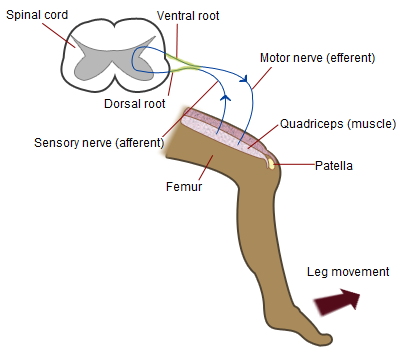
\includegraphics[width=1\linewidth]{imgs/Patellar-knee-reflex}

\end{floatright25}

One of Descartes core ideas was the concept of a reflex, which involves a clear-cut line of cause and effect between an impending stimulus or impulse, and a subsequent effect. A common example is the \href{https://en.wikipedia.org/wiki/Patellar_reflex}{knee-jerk reflex}, where tapping a knee in the right spot can cause a leg to automatically kick up a little bit.

\begin{floatleft25}
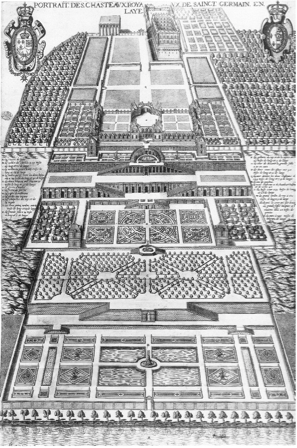
\includegraphics[width=1\linewidth]{imgs/st_germain}

\end{floatleft25}

In describing humans and animals as physical machines, Descartes was inspired by \href{https://en.wikipedia.org/wiki/Château_de_Saint-Germain-en-Laye\#16th–18th_centuries}{the gardens at Saint-Germain-en-Laye}.\footnote{\protect\hyperlink{ref-vaccariDissolvingNatureHow2012}{Vaccari, A., \& Philosophy Documentation Center. (2012). Dissolving {Nature}: {How Descartes Made Us Posthuman}. \emph{Techné: Research in Philosophy and Technology}, \emph{16}(2), 138--186. \url{https://doi.org/fz97nk}}.} The gardens were a marvel of hydraulic engineering. They contained an extensive network of pipes connected to fountains, and even controlled statues that had moving parts.

\begin{floatright50}
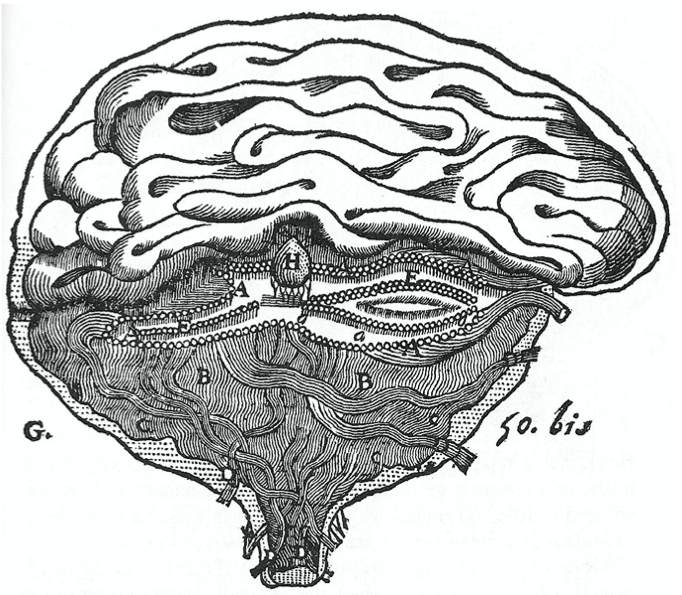
\includegraphics[width=1\linewidth]{imgs/Descartes_brain_large}

\end{floatright50}

Descartes made an analogy between the pipes in the garden and the physiology of the body and brain. For example, Descartes drew the brain as a complicated system of hydraulic pipes that were connected in a network of cause and effect reflexes. In the garden, water pushed through a pipe could cause a statue to move on the other end. In the body and brain, liquids pushed through the nervous system would cause movements too, in the form of behaviors and reflexes.

\hypertarget{pavlovs-liquid}{%
\subsection{Pavlov's liquid}\label{pavlovs-liquid}}

Pavlov considered the possibility that the brain could be an extremely complicated system of reflexes, with many input pathways connected to output pathways. Of Descartes idea he wrote,

\begin{quote}
``Our starting point has been Descartes' idea of the nervous reflex. This is a genuine scientific conception, since it implies necessity. It may be summed up as follows: An external or internal stimulus falls on some one or other nervous receptor and gives reise to a nervous impulse; this nervous impulse is transmitted along nerve fibres to the central nervous system, and here, on account of existing nervous connections, it gives rise to a fresh impulse which passes along outgoing nerve fibres to the active organ, where it excites a special activity of the cellular structures. Thus, a stimulus appears to be connected of necessity with a definite response, as cause with effect. It seems obvious that the whole activity of the organism should conform to definite laws.''
\end{quote}

Pavlov was interested in discovering the so-called laws of stimulus-response pathways in the brain that ultimately govern human and animal behavior. Whereas his contemporary Thorndike had used measurements of behavior (like how long it took to escape from a puzzle box) Pavlov took a more direct physiological measurement approach. He observed that organs near the brain were involved in secreting various liquids. For example, when a dog smells food, it may begin to salivate. The stimulus sensation of smelling food caused a cascade of events, like water moving through a complicated system of pipes, culminating in a salivation response. In his laboratory, Pavlov was studying saliva responses in dogs when he discovered these stimulus-response pathways were not as simple as hard-wired reflexes. Instead, Pavlov discovered what is now commonly termed ``classical conditioning'', a form of association learning linking together new stimulus-response pathways. For brevity, we will review a small subset of classical conditioning phenomena: simple acquisition, extinction, and spontaneous recovery. However, it is worth noting that Pavlov's results inspired a much larger discipline centered on associative learning phenomena that is beyond the scope of this book.

\hypertarget{simple-acquisition-and-conditioning-terminology}{%
\subsection{Simple acquisition and conditioning terminology}\label{simple-acquisition-and-conditioning-terminology}}

\begin{floatrightbox50}
\textbf{Simple acquisition procedure}

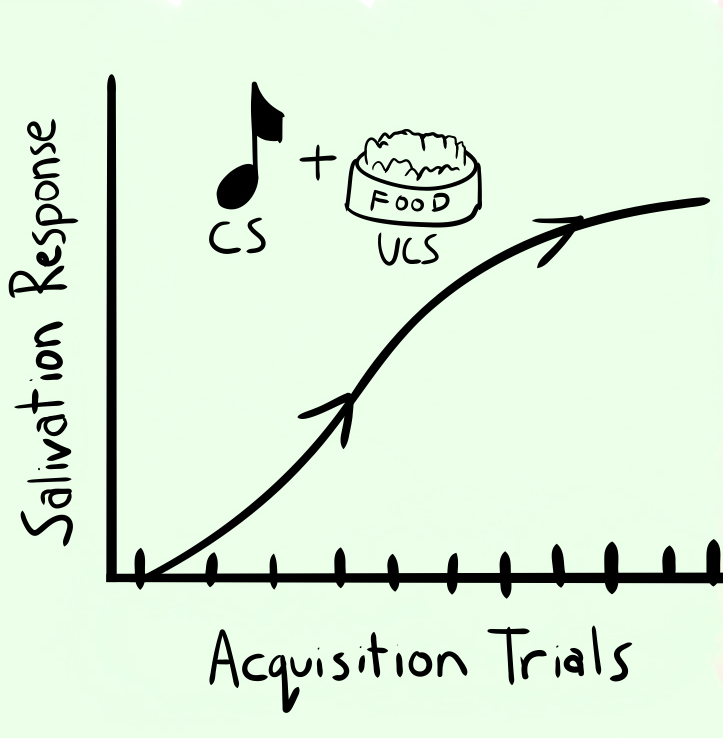
\includegraphics[width=1\linewidth]{imgs/Conditioning_Acquisition}

\end{floatrightbox50}

In Pavlov's simple acquisition procedure, a dog was housed in a controlled laboratory setting and given numerous ``acquisition trials''. On each trial, the dog was presented with a perceptual stimulus, like a loud tone, followed by a reward, like meat powder. The meat powder was a stimulus that normally caused the dog to salivate. Pavlov discovered that over the course of acquisition trials, the dog would begin to salivate in response to the loud tone, which was consistently paired with the food reward.

Simple acquisition is an example of a classical conditioning phenomena that results from systematic pairing of particular kinds of stimuli and their responses. Before we discuss a few other examples of conditioning phenomena, we will first define terms commonly used to describe stimuli and responses in these procedures. These terms include the unconditioned stimulus (UCS) and the unconditioned response (UCR), and the conditioned stimulus (CS) and the conditioned response (CR).

\begin{floatright50}
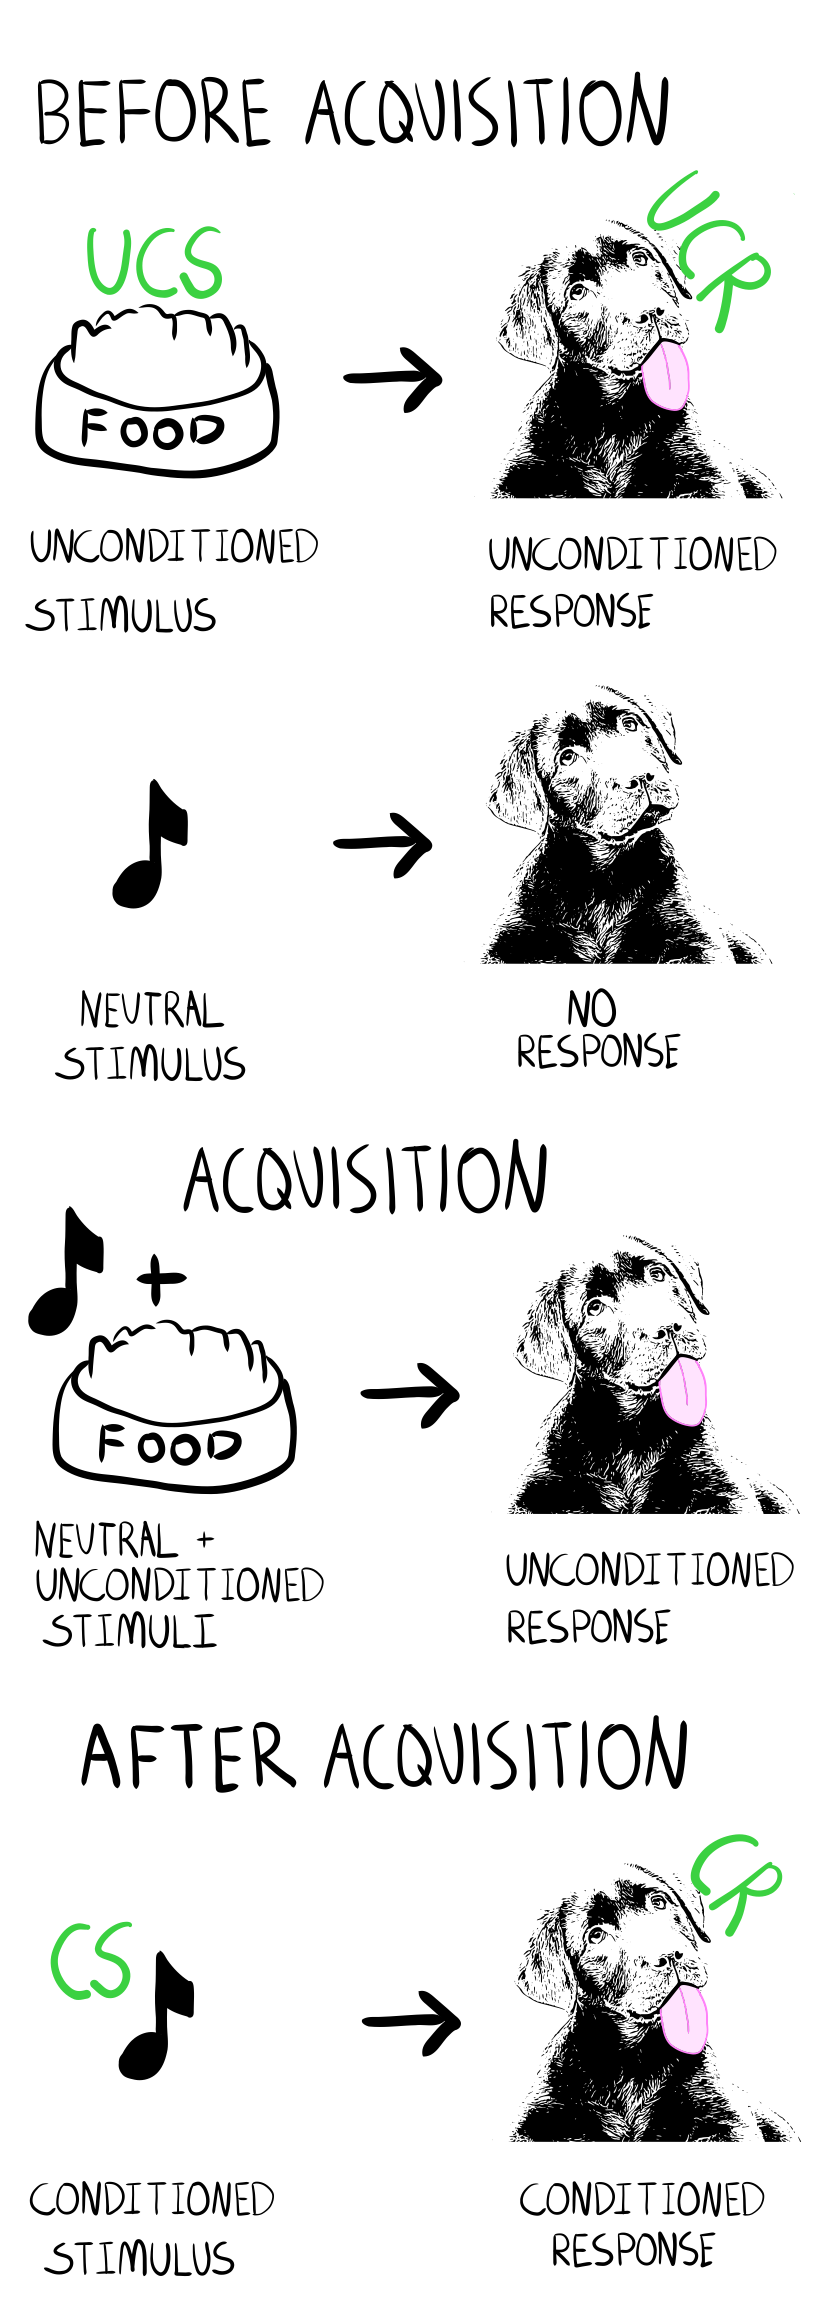
\includegraphics[width=1\linewidth]{imgs/Conditioning_terms}

\end{floatright50}

The unconditioned stimulus (UCS) evokes a response without any prior learning. For example, food stimuli such as food pellets or meat powder can be effective unconditioned stimuli because when animals salivate upon smelling the food. Importantly, an animal like a dog does not rely on any learning during the experiment to acquire this ability. Dog's come into the experiment with the ability to salivate in response to smelling food.

The unconditioned response (UCR) is the ``automatic'' or default response to an unconditioned stimulus. For example, salivating in response to smelling food is an unconditioned response.

Another example of an unconditioned stimulus is a small puff of air to an eyelid. If you have ever had a small puff of air blown onto your eye, what was your immediate reaction? Blinking is a common immediate reaction, and is another example of an unconditioned response.

The conditioned stimulus (CS) begins as a neutral perceptual stimulus that does not evoke the unconditioned response. For example, a loud tone or a bright light could become a conditioned stimulus. Importantly, in our example, before any acquisition trials, a loud tone would be considered a neutral stimulus because it would not evoke a salivation response (the UCR) in an animal.

During the acquisition trials the neutral stimulus is paired with the unconditioned stimulus. For example, the tone (neutral stimulus) is paired is paired with food (UCS). Across the acquisition trials the neutral stimulus (the tone) becomes the conditioned stimulus (CS) if it successfully begins to trigger the unconditioned response (UCR).

The conditioned response (CR) is the newly learned response evoked by the conditioned stimulus. For example, after a dog has acquired the association between hearing a tone and getting a food reward, the dog will begin to salivate in response to the tone. In this case, the conditioned stimulus (the tone) now evokes a conditioned response (salivating).

\hypertarget{explaining-simple-acquisition}{%
\subsubsection{Explaining simple acquisition}\label{explaining-simple-acquisition}}

In a simple acquisition procedure the animal appears to learn a new association. However, even the most basic phenomena of simple acquisition is not so simple to explain. For example, what kind of association was learned? Perhaps the tone made the animal expect to receive food, and the expectation for food evoked salivation. This kind of explanation could suggest that the neutral stimulus evokes something like a vivid mental image of eating delicious food, and the mental act of simulating the experience of eating delicious food is enough to somehow cause the salivation response. Notice also that this explanation itself is complicated because it invokes a concept of mental simulation, which itself is not a well-understood process, as part of the explanation. As an alternative, it is possible the neutral stimulus becomes directly associated with the salivation response. In this case, the neutral stimulus does not cause any mental images of eating delicious food, but it somehow directly causes salivation. It's also possible that both kinds of associations were learned.

\hypertarget{extinction}{%
\subsection{Extinction}\label{extinction}}

Can associations be unlearned? Pavlov addressed this question using an extinction procedure. The figure below shows an acquisition phase followed by an extinction phase. In the acquisition phase, the tone is paired with food, and over trials the dog begins to salivate when it hears the tone.

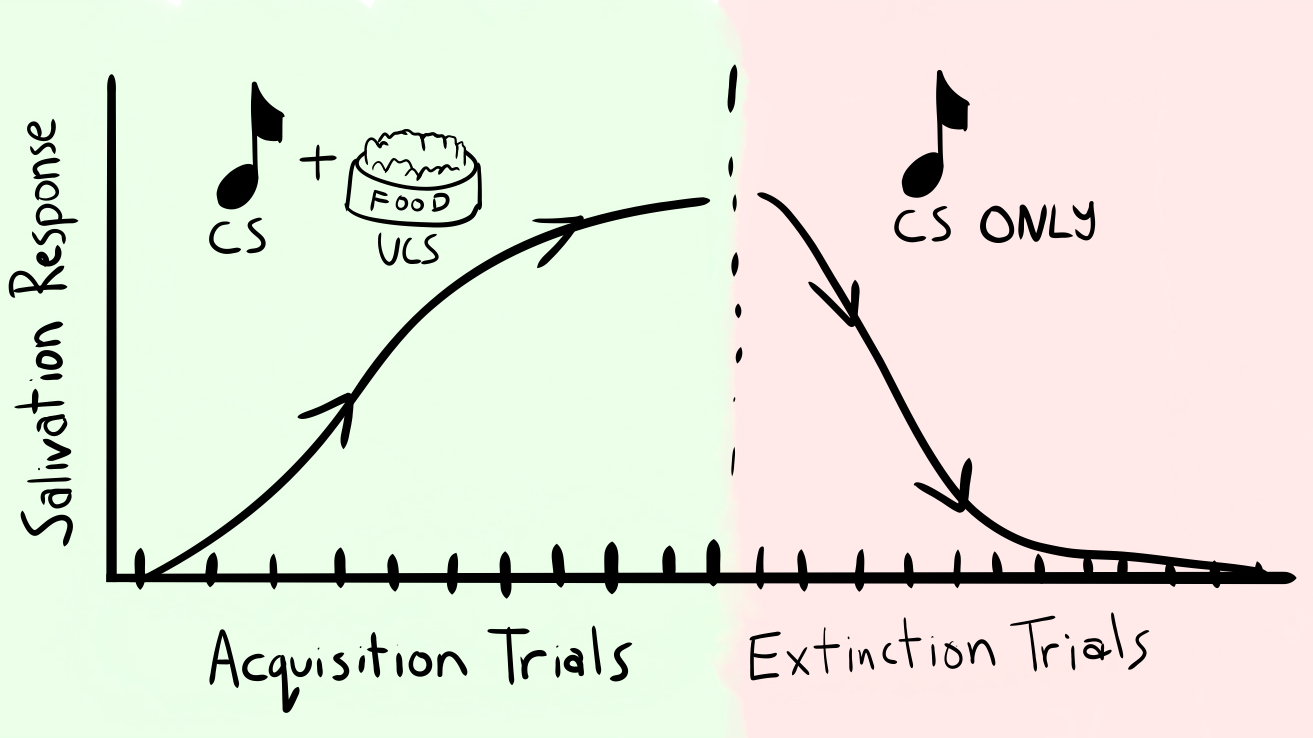
\includegraphics[width=1\linewidth]{imgs/Conditioning_extinction}

In the extinction phase, the CS is presented alone without any reward. At the beginning of the extinction phase, the dog shows the salivation response (UCR) when it hears the tone (CS). However, throughout the extinction phase, the dog will hear the tone many times, but the tone will not be paired with food reward. The phenomena of extinction occurs when the dog reduces or ceases to show a salivation response when it hears the tone. In other words, extinction is a reduction in the conditioned response (salivation) to the conditioned stimulus (tone).

\hypertarget{explaining-extinction}{%
\subsubsection{Explaining extinction}\label{explaining-extinction}}

The phenomena of extinction is very well-established. Animals who have acquired a new conditioned response to a conditioned stimulus will reliably show a reduction in the conditioned response following extinction training. Although the phenomena is well-established, the possible explanations of extinction are not as straightforward. For example, if an association was learned during acquisition, what happened to it during extinction? Was the original association unlearned or otherwise weakened? Perhaps the original association was untouched and the animal learned a new association during the extinction phase (e.g., that the tone does not predict food reward).

\hypertarget{spontaneous-recovery}{%
\subsection{Spontaneous Recovery}\label{spontaneous-recovery}}

Among several other conditioning phenomena beyond the scope of this chapter, Pavlov also discovered spontaneous recovery, which complicates the explanation of extinction learning. For example, above we briefly considered the possibility that extinction learning could reflect the undoing or unlearning of stimulus-response association.

For the moment, let's imagine that acquisition training causes an associative bond to form between a conditioned stimulus and response. Let's consider the bond like a string connecting the stimulus to the response. The learning process establishes a string-like connection between the conditioned stimulus and response, such that when the stimulus appears it ``pulls'' the connected response causing a particular behavior to occur.

Let's now imagine what happens to the string-like associative bond during the extinction phase. One possibility is that extinction causes the associative bond to deteriorate and weaken. In the metaphor, this would cause the string-like connection between conditioned stimulus and response to break down. Ultimately, if extinction learning was completely successful in breaking the connection, the previous association would be completely gone because the associative strands would be erased. As a result, after complete extinction learning the conditioned stimulus would never again evoke the conditioned response.

Pavlov's discovery of spontaneous recovery was a clue that extinction learning is not so simple. Spontaneous recovery refers to the phenomena that an extinguished conditioned stimulus can sometimes show a spontaneous recovery and evoke the conditioned response. Importantly, the extinguished conditioned stimulus has undergone an extinction procedure, and no longer causes the conditioned response. For example, a dog who had learned to salivate in response to a tone, and then received extinction training, would no longer salivate in response to the tone. Spontaneous recovery occurs when, sometime later, the dog appears to ``randomly'' or ``spontaneously'' begin salivating in response to the tone again.

According to the string-like explanation of associative-bonds above, spontaneous recovery should not be possible because the connection between conditioned stimulus and response should have been broken. Instead, the phenomena of spontaneous recovery invites alternative explanations. One possibility is that extinction does deteriorate an existing associative bond, but never perfectly. As a result, it is possible for the connection to spontaneously recover sometimes. Another possibility is that extinction is more about learning to suppress an already learned association. In this case, it is possible that the suppressive response deteriorates over time, allowing the original learned association to spontaneously recover. Another possibility is that learning is highly context-sensitive. As a result, extinction of a conditioned response may occur more strongly in the environment where the extinction training occurred, and the spontaneous recovery of the response may be more likely in other environments not associated with the extinction training.

\hypertarget{conclusions}{%
\section{Conclusions}\label{conclusions}}

This chapter introduced associationist ideas about cognition through early philosophy and early experimental psychology work on animals by Thorndike and Pavlov. The associationist philosophers were developing early process theories of how cognition works. A process theory includes a recipe of how individual parts interact together to produce some output. For associationists, the big claim about cognition was that it involved associative learning processes. These learning processes were assumed to create knowledge about the world by the process of experiencing events and objects in the world through sensory channels. Early experimental psychologists like Thorndike and Pavlov gave additional credence to the concept of associations as an acceptable unit of scientific study. Their laboratory methods, especially Pavlov's, inspired whole branches and schools of psychology interested in measuring associative learning processes, some of which have continued to the modern day. Throughout this textbook we will occasionally return to the literature on associative learning, which has succeeded in identifying numerous empirical phenomena and creating detailed mathematical process models of the association formation process; all of which are relevant to cognition--especially, if, as the associationists claimed, cognition is fundamentally about learning associations.

In the next two chapters we will visit two more major perspectives that lead into the emergence of modern cognitive psychology in the 1960s and 70s. Chapter 6 covers the school of behaviorism, and Chapter 7 covers the introduction of information theory to psychology.

\hypertarget{behaviorism}{%
\chapter{Behaviorism}\label{behaviorism}}

\begin{tabular}{r|l}
\hline
Word Count & Reading Time\\
\hline
12052 & 60.3 minutes\\
\hline
\end{tabular}

\hypertarget{overview}{%
\section{Overview}\label{overview}}

Last chapter introduced associationism as an example of early ideas about how processes of cognition might work. This chapter covers the school of behaviorism, which rose to prominence in American psychology in the early 20th century (roughly between 1920s to 1960s). Depending on who is telling the history, behaviorism could be the dark ages of psychology that stood in the way of modern cognitive psychology, or a fore-bearer paving the way.

This chapter describes the following attributes of behaviorism. First, an achievement of behaviorism was to legitimatize human and animal behavior as a topic of scientific inquiry in its own right. In this way, behaviorism carved out space between psychologies focused on intangible mental processes and physical brain-based processes. Second, behaviorism was constructed as a scientific system in the positivist tradition, which adds context to how I will present the goals and background ideas of the movement. Third, there were many versions of behaviorism because there were many researchers who developed and popularized their own brands. Fourth, perhaps because behaviorism was very large (occupying the time of many researchers), it is populated by controversial figures credited with creating and expanding the movement. The core claims and goals of behaviorism continue to have implications for the cognitive sciences and society in general today.

\hypertarget{the-rabbit-hole-to-explain-or-not-to-explain}{%
\section{The Rabbit Hole: To explain or not to explain?}\label{the-rabbit-hole-to-explain-or-not-to-explain}}

One of the goals of this textbook is to examine how empirical evidence is used to test and develop explanations about how cognition works. In my view, the task of explaining how cognition works is an important goal of research into cognitive abilities. Why is explanation important? I think there are several reasons. Tentative theories provide guidance and clues about how to focus research inquiries, and good explanations can lead to the development of useful applications and technologies. I also think that explanations are intrinsically interesting and worthwhile for understanding ourselves and our relationship to the world around us. At the same time, not everyone agrees that explanation is intrinsically important or useful.

For the moment, let's consider a fictional future where the science of cognition has been fully developed in great detail, with rock-solid explanations about how human and animal cognition works. Presumably, the theories and findings would have useful applications. Perhaps, the theories would explain new ways to help people restore lost cognitive abilities or expand upon existing cognitive abilities, or make machines capable of cognitive abilities. Although the basic science of cognition is interested in explaining cognition for reasons beside possible applications, it is clear that the ability to manipulate and control cognitive abilities is likely to emerge from a mature cognitive science capable of explaining how cognitive abilities work. Indeed, in the fictional future, it is easy to imagine that future societies maintained funding of cognitive science because of its high potential to discover methods to manipulate and control cognition, that could lead to new applied fields like cognitive engineering and technology. It is also easy to imagine that tools to manipulate and control cognition could be scary, especially if they were used for nefarious purposes. Finally, as some forms of behaviorism argued, it is possible to develop methods for manipulating and controlling cognition and behavior in the absence of theory and explanation.

\hypertarget{youtube-machine-learning-and-internet-behaviorism}{%
\subsection{Youtube, machine-learning, and internet behaviorism}\label{youtube-machine-learning-and-internet-behaviorism}}

The basic ideas of behaviorism have not disappeared, and they are being used in modern society in extraordinary ways to control and manipulate cognition and behavior. Let's start with a modern example to motivate a closer inspection of the history of behaviorism and its implications for understanding how cognition works.

The example is from a podcast called the \href{https://www.nytimes.com/column/rabbit-hole}{Rabbit Hole, by New York Times columnist Kevin Roose}. The series is generally about ``what the internet is doing do us?''. The first story in the podcast is a haunting account of how a young man's life was influenced in major ways by watching YouTube videos over a period of several years. How could watching YouTube videos have such a major impact on someone's life? The answer lies in the powerful behavior changing methods being deployed on the internet by many companies.

YouTube presents video content that users access through a web-browser. Web-browsers allow people to interact with the internet in many ways, like searching for content or clicking links on a webpage. Web-browsers also allow web-sites to embed code to harvest data about how people behave when they are on a website. For example, YouTube can store the history of videos that you watched, the order of videos that you clicked on, the amount of time spent watching each video, and many other kinds of user data (e.g., your location, your comment history, etc.). Furthermore, the behavioral data collected by websites can be combined with statistical techniques (like \href{https://en.wikipedia.org/wiki/Machine_learning}{machine learning}) to generate predictions about future user behavior.

YouTube collected massive amounts of video watching behavior data from their users, and then used advanced machine learning algorithms to predict and ultimately control and manipulate user behavior. For example, one goal was to improve the video recommendation algorithm, which seems like a useful goal for users of YouTube. Improving the recommendation algorithm would help users find content they wanted to watch--very practical. YouTube also had the goal of increasing the amount of time that people spent watching YouTube videos. If people watched more videos, then they would see more advertisements, and that would help YouTube's bottom line.

YouTube used the behavioral data they collected to generate predictions about what new videos to recommend to people in order to maximize their viewing time, and keep them watching YouTube videos as long as possible.

For some YouTube users, like the man in the podcast, the recommendation algorithm has deeply impacted their belief systems and behavior. For example, this user spent hours per day watching YouTube videos, many of which were selected by the recommendation algorithm. Initially, his viewing habits included searches for quirky music videos, but over time the algorithm suggested new content that increased his viewing time. This new content happened to politically polarizing content that became increasingly extreme on the far-right of the political spectrum. The user credits watching YouTube videos with his life decisions to become interested in and affiliated with white nationalist movements. Interestingly, the YouTube algorithm may also be involved in taking him in and out of this rabbit hole. For example, after becoming involved in far-right movements he continued to watch YouTube, which continued to suggest videos that would increase his viewing time. At this point in his viewing history, he became slightly more engaged by videos on the left-side of the political spectrum, and credits watching those videos with his decision to cease his involvement in far-right politics.

Although the cognitive sciences have been around for quite some time, there is no widely agreed upon theory or explanation of cognition that can be used to systematically control and manipulate behavior. Nevertheless, YouTube's algorithms that predict future viewing behavior from large databases of past viewing behavior appear highly successful in manipulating video watching times. In addition to the above anecdote, in 2017, the Wall Street Journal reported YouTube hit a new milestone--1 billion hours of YouTube had been watched in a single day \footnote{that's 41.6 million days worth of videos, or 114,155 years worth of video}. Viewing time had increased ten times from 2012, thanks to the introduction of predictive algorithms credited with driving the behavioral change. At the close of this chapter, we will return to the YouTube example to examine their algorithm as a modern case of implementing behavioral principles at massive scale. Next, we will examine the behaviorist approach to asking and answering questions about cognition.

\hypertarget{enter-behaviorism}{%
\section{Enter Behaviorism}\label{enter-behaviorism}}

The previous chapters described characters in the historical play of psychology that set the stage for the entry of behaviorism. I'll cast one group as the ``mentalists'' and the other group as the ``physicalists''. The mentalists were interested in examining so-called ``mental'' processes of cognition. For example, Galton assumed that subjective experiences of mental images was a real thing that differed among people, and that could be an object of scientific inquiry. Titchener had developed introspectionism, where people could be trained to carefully, systematically, and ``accurately'' describe their inner mental experiences; and, those experiences were regarded as worthy of scientific inquiry. Even Thorndike entertained the notion that animals experience mental simulations (e.g., about the possibility of food reward following escape from a puzzle box) that link associations between a stimulus situation and an eventual reward. The ``physicalists'' were interested in examining and understanding the physiological basis of psychological processes. For example, Pavlov's goal was to measure how stimulus-response learning processes were reflected in the production of glandular secretions. In the play, both sides criticized each other on several grounds-- the mentalists lacked objective measures and definitions, the physiologists were too reductive and weren't studying cognition.

I'll add a few additional backdrops framing the entry of behaviorism.
One backdrop I term scientific credentialism, which involves making claims about the kind of credentials that a field of study must possess in order to be considered a ``true'' science; and, for psychology, a concern, even obsession, with claiming possession of those credentials so that it would be recognized by society and other sciences as a proper science in its own right. The concern that psychology should become a science is related to the backdrops of \href{https://en.wikipedia.org/wiki/Positivism}{positivism}, and scientific \href{https://en.wikipedia.org/wiki/Utopia\#Utopianism}{utopianism}. There are many philosophies of science that define the credentials of science in different ways, and prominent strains of behaviorism were constructed in the positivist tradition. Scientific utopianism refers broadly to the notion that society can be improved through science and technology. I briefly discuss positivism and scientific utopianism before we turn to the main act\ldots behaviorism.

\hypertarget{positivism}{%
\subsection{Positivism}\label{positivism}}

\begin{floatright25}
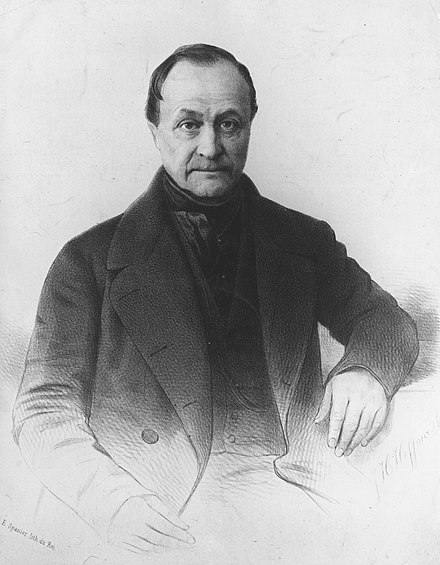
\includegraphics[width=1\linewidth]{imgs/Auguste_Comte}

\end{floatright25}

\href{https://plato.stanford.edu/entries/comte/}{Auguste Comte} (1798--1857) created positivism as a part of founding \href{https://en.wikipedia.org/wiki/Sociology}{sociology}. He was a French philosopher writing during a period of social upheaval \footnote{e.g., the \href{https://en.wikipedia.org/wiki/Revolutions_of_1848}{1848 French revolution} to remove the monarchy}. His work is an early example of a \href{https://en.wikipedia.org/wiki/Philosophy_of_science}{philosophy of science} attempting to define attributes and processes of science, as well as hierarchical relations between scientific disciplines. He argued that science and society develops through theological, metaphysical, and positive stages to explain natural phenomena. In the theological phase, phenomena are explained by supernatural powers. For example, the mind is attributed to soul or spiritual forces. The metaphysical stage replaces the supernatural forces with abstractions. For example, the mind is psychic forces. In the positive stage a description system is achieved, whereby the scientific process will eventually describe the nouns and verbs of a phenomena. The nouns are the features of a phenomena, and the verbs are the mathematical laws that describe actions of the features. For example, the work of B.F. Skinner (at the end of this chapter), is an example of reducing cognition and behavior to a descriptive system in the positive tradition.

\hypertarget{scientific-utopianism}{%
\subsection{Scientific Utopianism}\label{scientific-utopianism}}

Utopias take on many forms. In literature, \href{https://en.wikipedia.org/wiki/List_of_utopian_literature}{writers} have envisioned more perfect utopian societies. In America, numerous attempts at \href{https://en.wikipedia.org/wiki/List_of_American_utopian_communities}{utopian communities} have been made over centuries. Similarly, utopias have routinely been envisioned in academic discourse. For example, working with \href{https://en.wikipedia.org/wiki/Henri_de_Saint-Simon}{Henri Saint-Simon} Auguste Comte extended his views on positivism to society at large, and envisioned utopic societies that would embrace scientific understanding and follow the motto of positivism: ``Love as a principle and order as the basis; progress as the goal'' \footnote{Social discourse in Brazil was influenced by positivism and Ordem and Progresso remains the national motto}. Comte also proposed a humanistic religion based on science to replace the Catholic church.

Comte's ideas were popularized in England through \href{https://en.wikipedia.org/wiki/John_Stuart_Mill}{John Stuart Mill}, who published ``Auguste Comte and Positivism'' in 1865. Coincidentally, 1865 was the same year that Galton published his first paper on eugenics.\footnote{\protect\hyperlink{ref-galtonHereditaryTalentCharacter1865}{Galton, 1865}.} Like Comte, Galton envisioned a utopic future where society could be improved through eugenics. Galton also proposed that eugenics attain the status of science and religion. Unfortunately, like so many fictional utopias that turned dystopic, as previous chapters have discussed, the real-world movement of eugenics led to many injustices. The rise of behaviorism in psychology coincided with the eugenics movement, and many behaviorists were committed to eugenics. Additionally, on occasion, behaviorism was forwarded by a few prominent psychologists as a scientific method to achieve utopias through social engineering.

\hypertarget{associationism-conditioning-and-behaviorism}{%
\section{Associationism, Conditioning and Behaviorism}\label{associationism-conditioning-and-behaviorism}}

\begin{floatrightbox50}
Robert Yerkes was a eugenicist and APA president who conducted the alpha-beta intelligence tests of the American military in World War I. He was also a comparative psychologist and studied animal cognition. Pavlov also became interested in eugenics (even after eugenics journals were outlawed in Russia in the 1920s), and conducted experiments on inheritance of temperament in dogs.\footnote{\protect\hyperlink{ref-rossiianovIvanPavlovMoral2017}{Rossiianov, K., \& Seay, N. (2017). Ivan {Pavlov} and the {Moral Physiology} of {Self}. \emph{Kritika: Explorations in Russian and Eurasian History}, \emph{18}(1), 203--209. \url{https://doi.org/gk92h3}}.}

\end{floatrightbox50}

The more immediate backdrops to behaviorism were covered in the last chapter, these are the ideas of associationism and the discovery of classical conditioning by Pavlov. Pavlov's extended lectures on his work were translated in to English in 1927, however his methods were introduced to American psychologists much earlier. Pavlov won the Nobel prize in 1904 for his conditioning work in physiology; and in 1909, Yerkes and Margulis\footnote{\protect\hyperlink{ref-yerkesMethodPawlowAnimal1909}{Yerkes, Robert M., \& Morgulis, S. (1909). The method of {Pawlow} in animal psychology. \emph{Psychological Bulletin}, \emph{6}(8), 257. \url{https://doi.org/fkvq8h}}.} published descriptions of his methods in ``The method of Pawlow in animal psychology'' \footnote{In this publication Ivan P. Pavlov was written as J. P. Pawlow.}.

Pavlov's methods and findings arrived in America at the same time that psychologists were aiming to establish themselves as a real science. Psychologists were already investigating associative processes in animal cognition (e.g., Thorndike), and humans using reaction times (e.g., Cattell). And, perhaps the physiological nature of Pavlov's methods appeared attractive as a ``more scientific'' way to measure associative learning. It is certainly the case that Pavlovian conditioning was inspirational to \href{https://en.wikipedia.org/wiki/John_B._Watson}{John B. Watson} (1878-1958), the ``arch-prophet'' \footnote{according to Tolman} of Behaviorism. As we will cover shortly, Watson's behaviorism consisted of grand claims that psychology should become a science of stimulus-response learning.

In the remaining sections, instances of behaviorism are explored further by examining prominent individuals and their individual flavors of behaviorism. There were/are many behaviorists, but this chapter limits discussion to J. B. Watson, \href{https://en.wikipedia.org/wiki/Edward_C._Tolman}{Edward Tolman} (1886--1959), \href{https://en.wikipedia.org/wiki/Clark_L._Hull}{Clark L. Hull} (1884-1952) and \href{https://en.wikipedia.org/wiki/B._F._Skinner}{Burrhus F. Skinner} (1904--1990).

\hypertarget{watsons-salesman-behaviorism}{%
\section{Watson's ``Salesman'' Behaviorism}\label{watsons-salesman-behaviorism}}

\begin{floatright25}
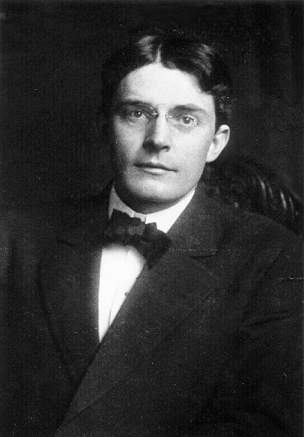
\includegraphics[width=1\linewidth]{imgs/John_Broadus_Watson}

\end{floatright25}

J. B. Watson is one of the controversial figures I alluded to earlier. He is credited with ushering in behaviorism, and although he did push it in, he also left psychology soon after.

Watson completed his Ph.D.~at the University of Chicago in 1903. By 1908, he became chair of the Psychology department at Johns Hopkins University. In 1913, he launched a critique of introspectionist methodology in his ``Behaviorist Manifesto'' titled, ``Psychology as the Behaviorist Views it.''\footnote{\protect\hyperlink{ref-watsonPsychologyBehavioristViews1913}{Watson, John B. (1913). Psychology as the behaviorist views it. \emph{Psychological Review}, \emph{20}, 158--177}.} Watson became APA president in 1915, and in the society meeting that year he argued that psychology should adopt the methods of Pavlov to become a science of conditioned reflexes and stimulus-response learning.\footnote{\protect\hyperlink{ref-watsonPlaceConditionedreflexPsychology1916}{Watson, John B. (1916). The place of the conditioned-reflex in psychology. \emph{Psychological Review}, \emph{23}(2), 89. \url{https://doi.org/bdw5ns}}.}

Watson published some work on conditioned reflexes, but is most infamous for his ``\href{https://en.wikipedia.org/wiki/Little_Albert_experiment}{Little Albert}'' experiment in 1920, which was an attempt to generalize Pavlovian conditioning to humans.\footnote{\protect\hyperlink{ref-watsonConditionedEmotionalReactions1920}{Watson, John B., \& Rayner, R. (1920). Conditioned emotional reactions. \emph{Journal of Experimental Psychology}, \emph{3}(1), 1. \url{https://doi.org/b9k9ng}}.} This study was conducted before ethical standards for protecting human subjects in research, like those in the \href{https://en.wikipedia.org/wiki/Belmont_Report}{Belmont Report}, were codified and enforced in America. The experiment was supposed to have two phases, but only the first phase was conducted. In the baseline phase, an eleven month old infant (``little Albert'') was exposed to stimuli such as a white rat, rabbit, dog, masks, burning newspapers and shown to elicit no fear response. During the fear-conditioning phase, whenever the infant was shown a white rat, Watson created a loud sound by striking a steel bar with a hammer. This caused the infant to become very distressed (crying, crawling away). Watson continued to ``condition'' the infant in this manner until he became afraid of the white rat in the absence of the sound. Watson went on to measure the infant becoming distressed to other objects in an apparent demonstration of generalized fear-conditioning. Watson apparently planned to ``de-sensitize'' the infant, using an extinction procedure. However, the infant was removed from the hospital where Watson was conducting his study before the planned de-sensitization could take place.

Also in 1920, Watson was fired from his position at John Hopkins as a part of a divorce scandal. He took an advertising job in New York and did not continue as an academic. However, he continued to publish popular science books, such as ``Behaviorism'' in 1924, and books on using behaviorist techniques for parenting.

Watson's role in psychology can take on a positive light. In 1957, shortly before his death, he received the gold medal from the American Psychological Association for his contributions to the field. Proponents of the modern field of \href{https://en.wikipedia.org/wiki/Applied_behavior_analysis}{applied behavior analysis} have argued that historical descriptions of Watson's views that appear in textbooks have been inaccurate, and should be corrected so that Watson can be better appreciated.\footnote{\protect\hyperlink{ref-toddWhatPsychologyHas1994}{Todd, J. T. (1994). What {Psychology Has} to {Say About John B}. {Watson}: {Classical Behaviorism} in {Psychology Textbooks}, 1920-1989. In J. T. Todd \& E. K. Morris (Eds.), \emph{Modern perspectives on {John B}. {Watson} and classical behaviorism} (pp. 75--107). {Greenwood Press}}.} For example, in the 1970s many textbooks published claims that Watson was conducting early experiments in sex research while having an affair with his graduate student. However, historical research into those allegations have been inconclusive.\footnote{\protect\hyperlink{ref-benjaminJohnWatsonAlleged2007}{Benjamin, L. T., Whitaker, J. L., Ramsey, R. M., \& Zeve, D. R. (2007). John {B}. {Watson}'s {Alleged Sex Research}: {An Appraisal} of the {Evidence}. \emph{American Psychologist}, \emph{62}(2), 131--139. \url{https://doi.org/b95f2v}}.}

Watson has also been presented in a very negative light. For example, in the book \emph{Scientific Pollyannaism}, Yakushko describes Watson as an advocate of eugenics, and that his research was ``filled with what could be described as sadistic experiments on infants and young children, many of whom Watson acknowledges to be orphans or children who were institutionalized under his care at a children's hospital.''\footnote{\protect\hyperlink{ref-yakushkoScientificPollyannaismInquisition2019}{Yakushko, O. (2019b). \emph{Scientific {Pollyannaism}: {From Inquisition} to {Positive Psychology}}. {Springer International Publishing}. \url{https://doi.org/10.1007/978-3-030-15982-5}}.} Watson was listed as new active researcher in the ``Eugenics Research Association'' by the publication Eugenical News, but he was kicked out of that association as well when we has fired during his divorce.

Watson wrote widely on behaviorist techniques that parents could use to raise more superior children. These writings reiterated themes from eugenics on how superior parents can breed superior children, but allowed space for behaviorist interventions to play some role for gifted parents to nurture their children into even more gifted beings than would be possible by genetics alone. For example, the following quote appears in a book co-authored by Watson.

\begin{quote}
``Superior parents have no guarantee that their children will be superior. No one can predict the qualities that will arise from their combination, for millions of possibilities are equally open. Superior parents must watch and help their children with the same anxious care that others must use. Of course we know that gifted parents are much more likely to produce gifted children, inferior parents inferior children.''\footnote{\protect\hyperlink{ref-jenningsSuggestionsModernScience1918}{Jennings, H. S., Watson, J. B., Meyer, A., \& Thomas, W. I. (1918). \emph{Suggestions of modern science concerning education}. {Macmillan}}.}
\end{quote}

Although Watson left academia when he was fired in 1920, he did not stop experimenting on children. Instead, he wrote about applying his behaviorist techniques on his own children, and described thought-experiments where he wished he could electrify his son Billy's toys, and then shock the other son Jimmy when ever he tried to touch them, as a way to teach him to avoid Billy's toys.\footnote{\protect\hyperlink{ref-watsonPsychologicalCareInfant1928}{Watson, John Broadus. (1928). \emph{Psychological care of infant and child.}}} Paraphrasing from Yakushko,\footnote{Pg 107, \protect\hyperlink{ref-yakushkoScientificPollyannaismInquisition2019}{Yakushko, 2019b}.} she discusses family survivors of Watson's experimentation and notes that his children claimed they were damaged by his behaviorist parenting: Polly Watson became an alcoholic and was regularly hospitalized for suicide attempts. John Watson died of a bleeding ulcer that he attributed to his father's feeding schedule. William Watson published scathing personal letters about his fathers abuse in Life Magazine. Billy Watson committed suicide in his 30s. James Watson, the youngest son, became a vocal critic of his father and gave public interviews about recovering from Watson's abuse.

\hypertarget{elements-of-watsons-behaviorism}{%
\subsection{Elements of Watson's Behaviorism}\label{elements-of-watsons-behaviorism}}

Watson coined the term behaviorism in 1913\footnote{\protect\hyperlink{ref-schneiderHistoryTermRadical1987}{Schneider, S. M., \& Morris, E. K. (1987). A {History} of the {Term Radical Behaviorism}: {From Watson} to {Skinner}. \emph{The Behavior Analyst}, \emph{10}(1), 27--39. \url{https://doi.org/c9wz}}; \protect\hyperlink{ref-watsonPsychologyBehavioristViews1913}{John B. Watson, 1913}.} and left academia in 1920, taking up a sales position in New York City. However, he continued to express and sell his behaviorism by publishing popular science books, such as ``Behaviorism.''\footnote{\protect\hyperlink{ref-watsonBehaviorism1924}{Watson, John B. (1924). \emph{Behaviorism}. {W. W. Norton \& Company}}, which was published in several revisions up to 1958.} On my reading of Watson, the elements of his behaviorism are largely ideological and often flamboyant. I attempt a summary of his views, and then provide a few quotes.

Watson was concerned that psychology was not scientific enough. He criticized introspectionist methods because they did not provide objective and verifiable measures. He promoted Pavlov's discovery of conditioned reflexes as the new empirical strategy that would make psychology a real science; and, argued that psychology could be reduced to associative learning of stimulus-response relationships. He argued behaviorism's scientific goal was to establish empirical laws that would enable control and manipulation over stimulus-response learning. He envisioned behaviorism's societal goal as creating new applied fields like behavioral engineering, and a new behaviorist religion based on scientific ethics. There is a strong parallelism to the scientific utopianism of eugenics. Watson was a member of eugenics organizations, and although he later criticizes aspects of eugenics (notably after his membership was removed), he offered behaviorism as a supplement rather than wholesale replacement of eugenics. For example, eugenics was concerned with improving humans over generations from the side of genetic inheritance. Watson did not deny the role of genetic influences, but saw an opportunity to promote his behaviorism as the scientific way to improve humans within a generation from the perspective of environmental or learned influences. In this way, nature and nurture could be controlled and manipulated through eugenics and behaviorism to create a more perfect society.

\hypertarget{watsons-stimulus-response-positivism}{%
\subsection{Watson's stimulus-response positivism}\label{watsons-stimulus-response-positivism}}

In his book Behaviorism, Watson follows Comte's positivism to criticize psychology and replace it with behaviorism. He argues that introspective psychology had a strong religious background (e.g, Comte's theological stage), invoking God-concepts to explain the mind; and, that appeals to abstract entities like consciousness were unscientific (e.g., Comte's metaphysical stage). He then advanced behaviorism as the proper scientific discipline (the positive stage).

Watson defined behaviorism as, ``a natural science that takes the whole field of human adjustments as its own\ldots{[}and that while it is interested in the physiology of parts of humans and animals it{]}\ldots is intrinsically interested in what the whole animal will do from morning to night and form night to morning''.

He further explains that ``the interest of the behaviorist in man's doings is more than the interest of the spectator--he wants to control man's reactions as physical scientists want to control and manipulate other natural phenomena. It is the business of behavioristic psychology to be able to predict and to control human activity. To do this it must gather scientific data by experimental methods. Only then can the trained behaviorist predict, given the stimulus, what reaction will take place; or, given the reaction, state what the situation or stimulus is that has caused the reaction.''

\hypertarget{watsons-s-r-system}{%
\subsection{Watson's S-R System}\label{watsons-s-r-system}}

In positivism a descriptive scientific system is achieved when there are terms for describing features of a phenomena, and functions describing actions of the features, such that they come under predictable control. Watson saw the possibility for stimulus-response learning to become such a system. Elements of Watson's S-R system are described below with figures showing original text.\footnote{From, \protect\hyperlink{ref-watsonBehaviorism1924}{John B. Watson, 1924}.}

\begin{floatrightbox50}
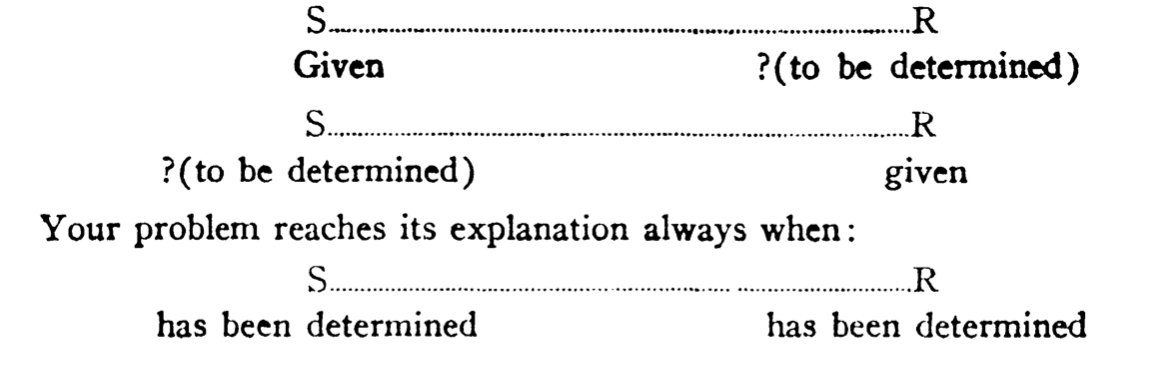
\includegraphics[width=1\linewidth]{imgs/Watson_SR}

\end{floatrightbox50}

Stimuli (in the environment) and responses (observable behaviors of humans and animals) and were both identifiable, and according to the idea of associationism, were linked together. Watson stated the problem for behaviorism as finding the functional relationship between stimuli and responses, such that one could be predicted or ascertained from the other.

One set of behaviors involved pre-existing stimulus-response associations in the form of unconditioned responses.

\begin{center}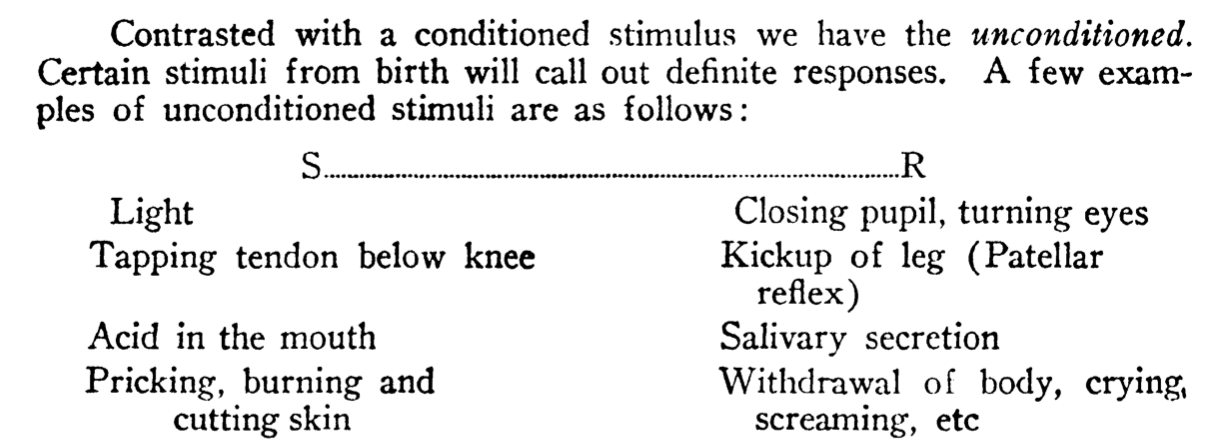
\includegraphics[width=1\linewidth]{imgs/Watson_unconditioned} \end{center}

All remaining behavior was involved newly acquired or learned stimulus-responses associations. Watson generalized Pavlov's concept of conditioning to cover learned behaviors. He presented conditioning as a widely applicable process that could potentially allow a wide-range of stimuli to become a substitute for triggering a wide-range of responses.

\begin{center}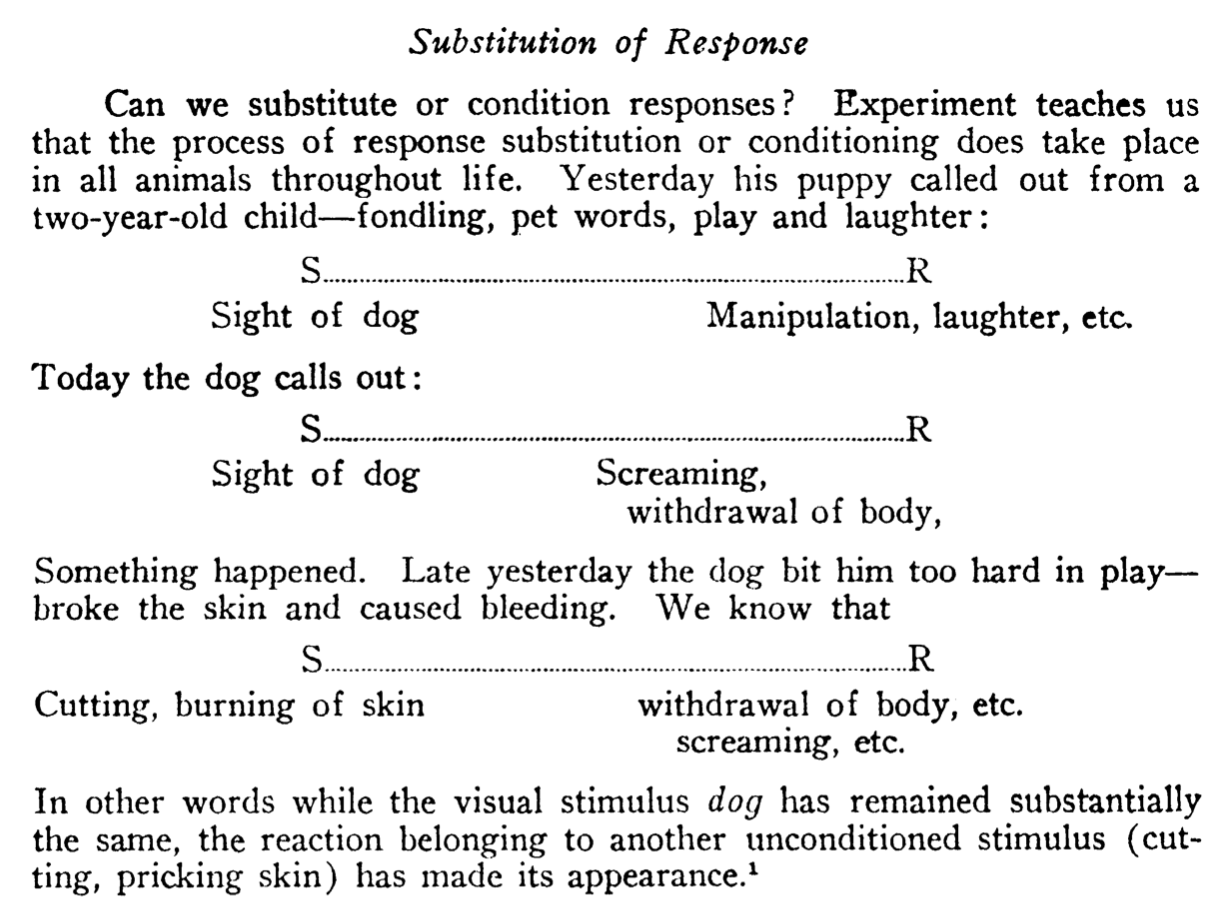
\includegraphics[width=1\linewidth]{imgs/Watson_conditioned} \end{center}

Watson's S-R system was more like speculative fiction than a fully worked out system in the positivist tradition. He identified terms like stimuli and response, and made grand claims about possible functional relationships between them, but did not supply a detailed mathematical analysis of assumed lawful connections between stimuli and responses. Instead, he jumped straight to envisioning how future society could control its citizenry using behavioral engineering. He formulated societal level manipulations in terms of stimulus-response questions (see below), and was hopeful that behaviorism could help make predictions about outcomes of such interventions.

\begin{center}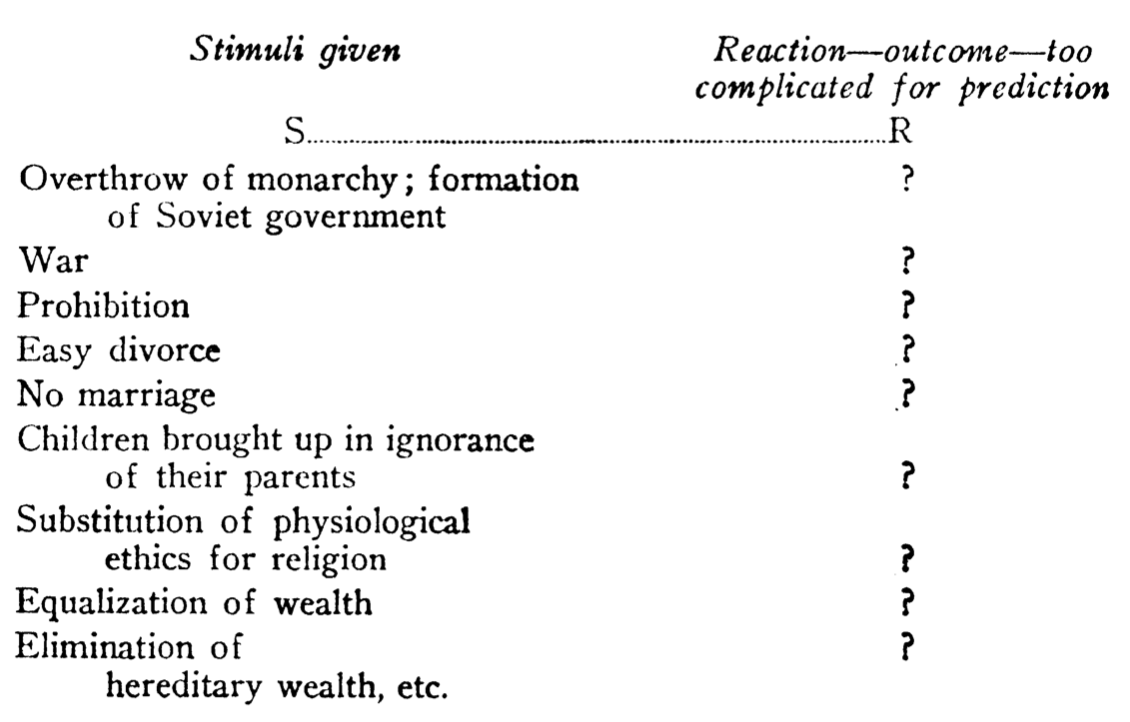
\includegraphics[width=1\linewidth]{imgs/Watson_Society_S} \end{center}

Similarly, he imagined desired outcomes for society, and implied that behavioral engineering would be able to construct the appropriate stimuli to force the behaviors he considered desirable.

\begin{center}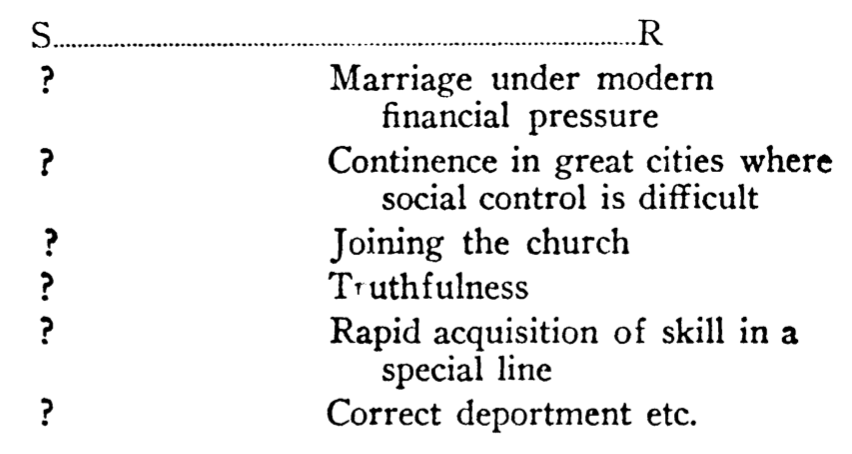
\includegraphics[width=1\linewidth]{imgs/Watson_Society_R} \end{center}

Finally, Watson promoted behaviorism as more than the correct scientific way to do psychology. It was an academic social movement, in the tradition of scientific utopias, that was sweeping the nation. For example, in the figure below, Watson describes how psychology, philosophy, ethics, social psychology, sociology, religion, and psycho-analysis were all becoming behaviorist systems or disappearing if they were not.

\begin{center}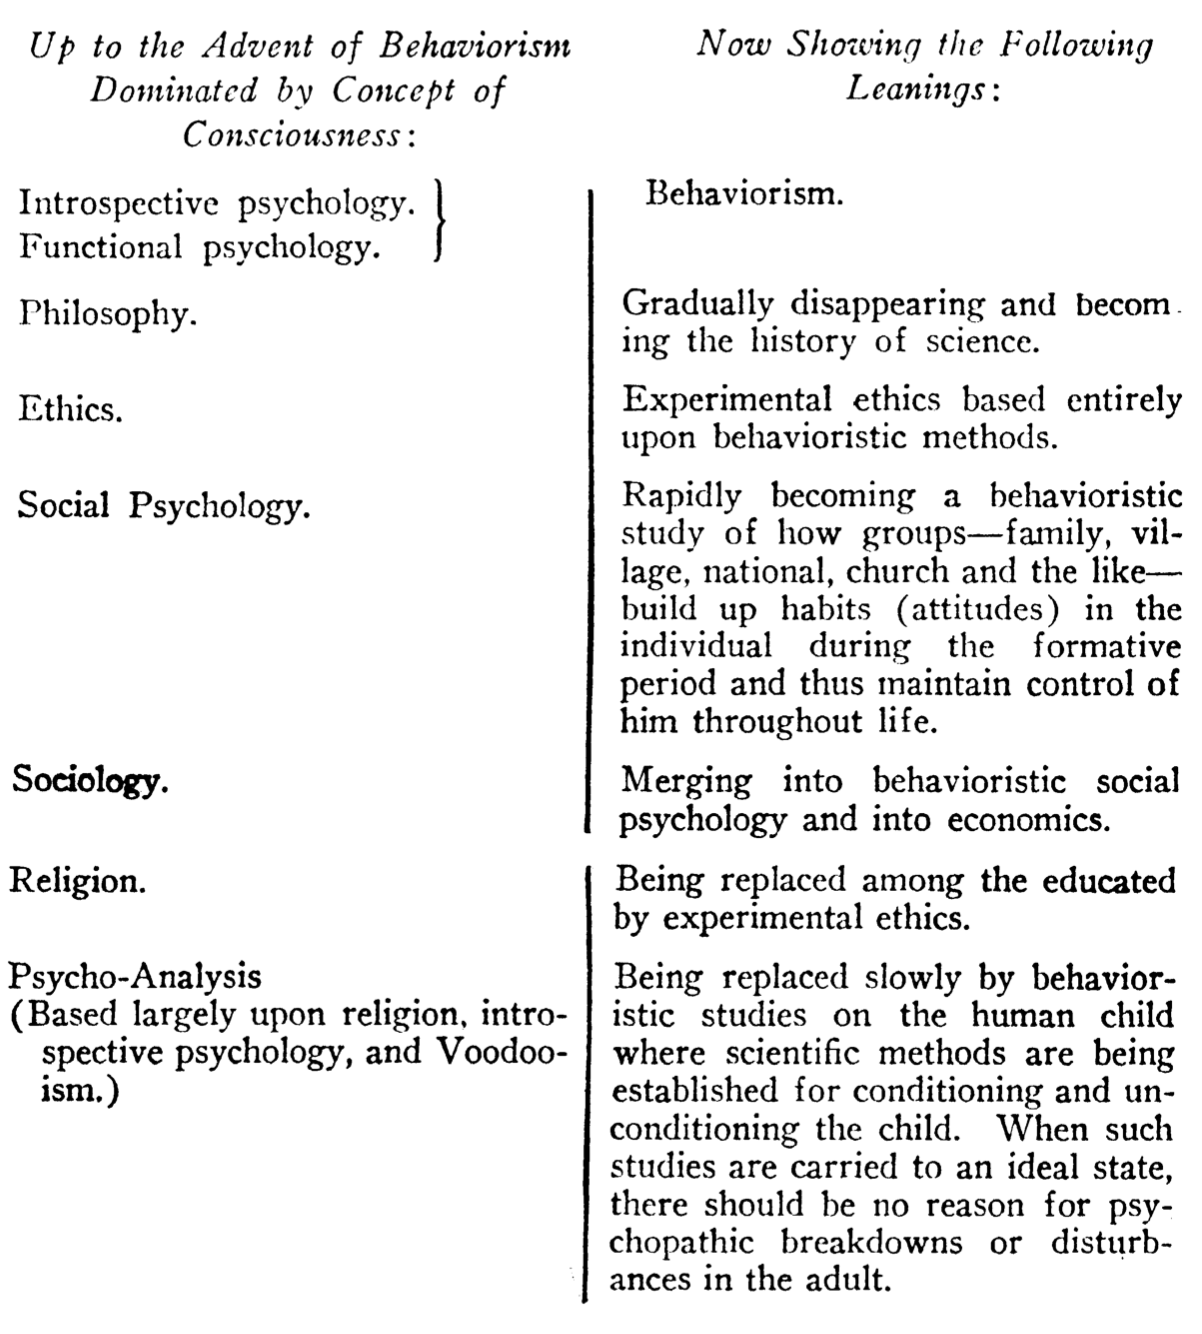
\includegraphics[width=1\linewidth]{imgs/Watson_sweep} \end{center}

\hypertarget{tolmans-purposive-behaviorism}{%
\section{Tolman's ``Purposive'' behaviorism}\label{tolmans-purposive-behaviorism}}

\begin{quote}
``All students agree as to the facts. They disagree, however, on theory and explanation.'' -- Tolman, 1948\footnote{\protect\hyperlink{ref-tolmanCognitiveMapsRats1948}{Tolman, Edward C. (1948). Cognitive maps in rats and men. \emph{Psychological Review}, \emph{55}(4), 189--208. \url{https://doi.org/10.1037/h0061626}}.}
\end{quote}

\begin{floatright25}
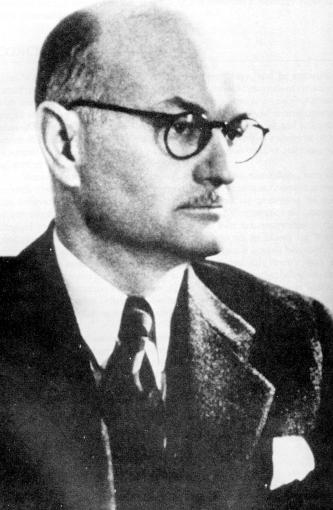
\includegraphics[width=1\linewidth]{imgs/Tolman_portrait}

\end{floatright25}

\href{https://en.wikipedia.org/wiki/Edward_C._Tolman}{Edward C. Tolman's} (1886-1959) flavor of behaviorism incorporated elements that are common in modern cognitive psychology. In 1932, he wrote ``Purposive Behavior in Animals and Men,''\footnote{\protect\hyperlink{ref-tolmanPurposiveBehaviorAnimal1932}{Tolman, E. C. (1932). \emph{Purposive behavior in animal and men}. {The Century Co.}}} which summarizes his research and views on behaviorism. In presenting his view, Tolman points out that numerous authors, such as ``Holt, Perry, Singer, de Laguna, Hunter, Weiss, Lashley'' had been developing their own versions of behaviorism, and refers to Roback's ``Behaviorism and Psychology'', for ``the best analysis and bibliography of the different varieties of behaviorims extant to 1923''. I mention the diversity of views to emphasize the difficulty of treating the period of behaviorism as single monolithic entity. Instead, much like there are numerous views on cognition today, there were numerous views on behaviorism. Similarly, it is worth noting that there were many non-behaviorist views on psychology and non-behaviorist lines of research that were ongoing throughout the so-called period of behaviorism.

After some training in Germany, Tolman received his Ph.D.~at Harvard under \href{https://en.wikipedia.org/wiki/Edwin_Holt}{Edwin Holt} in 1915, who had worked under \href{https://en.wikipedia.org/wiki/Hugo_Münsterberg}{Hugo Munsterberg}. He is well-known for his research on maze-learning in rats, which is the focus of this section.

\hypertarget{molar-definition-of-behavior}{%
\subsection{Molar definition of behavior}\label{molar-definition-of-behavior}}

Tolman suggested that Watson had given a ``molecular'' definition of behaviorism, which supplied important units like stimulus and response, and reduced behavior to ``strict physical and physiological muscle-twitches''. Tolman \footnote{and others, Holt, de Laguna, Weiss} argued in favor of a ``molar'' definition of behaviorism, which is the idea that behaviors are things in and of themselves that could be studied, irrespective of their ``molecular'' units. To quote from Tolman:

\begin{quote}
``An act qua `behavior' has distinctive properties all its own. These are to be identified and described irrespective of whatever muscular, glandular, or neural processes underlie them. These new properties, thus distinctive of molar behavior, are presumably strictly correlated with and, if you will, dependent upon, physiological motions. But descriptively and per se they are other than these motions.''
\end{quote}

\begin{quote}
``A rat running a maze, a cat getting out of a puzzle box, a man driving home to dinner, a child hifing from a stranger, a woman doing her washing or gossiping over the telephone, a pupil marking a mental test sheet, a psychologist reciting a list of nonsense syllables, my friend and I telling one another our thought and feelings-- these are behaviors (qua molar). And it must be noted that in mentioning no one of them have we referred to, or, we blush to confess it, for the most part even known, what were the exact muscles and glands, sensory nerves, and motor nerves involved. For these responses somehow had other sufficiently identifying properties of their own.''
\end{quote}

\hypertarget{purposive-and-cognitive-determinants}{%
\subsection{Purposive and cognitive determinants}\label{purposive-and-cognitive-determinants}}

Watson's stimulus-response behaviorism identify S and R as the important objective units of analysis, and they neglect or deliberately ignore the purpose of behavior, and potential cognitive processes intervening between perception of a stimulus and final production of a response. In suggesting that behavior should be studied as a wholisitic molar unit in and of itself, Tolman further argued that additional terms were necessary to describe the purposes and cognitive mechanisms of behavior. In some sense, Tolman's ideas appeared to revisit the intangible mental operations that inspired behaviorist critiques of ``mentalist'' psychology. However, Tolman also proceeded in the positivist tradition and was at pains to clarify that his new terms were intended only as descriptors. For example, just like it would be OK to describe a stimulus as being ``green'', without implying anything about an inner mental experience of seeing a green object; Tolman thought it would be useful and necessary for a science of behavior to describe behaviors as having purposes and cognitions--but only for descriptive purposes, and not to imply the inner mental processes.

The following quotes show Tolman building his argument to use terms for purpose and cognition to more fully describe behavior.

\begin{quote}
``Behavior in our sense, always seems to have the character of getting to or getting-from a specific goal object, or goal situation. The complete identification of an single behavior act requires, that is, a reference first to some particular goal object or objects which that act is getting to, or, it may be, getting from, or both. Thus, for example, the rat's behavior of''running the maze'' has as its first and perhaps most important identifying feature the fact that it is a getting to food''.
\end{quote}

\begin{quote}
``To sum up, the complete descriptive identification of any behavior act per se requires descriptive statements relative to (a) the goal-object or objects, being got to or from, (b) the specific pattern of commerces with means-objects involved in this getting to or from, and (c) the facts exhibited relative to the selective identification of routes and means-objects as involving short (easy) commerces with means-objects for thus getting to or from''
\end{quote}

\begin{quote}
``But surely any''tough minded'' reader will by now be up in arms. For it is clear that thus to identify behaviors in erms of goal-objects, and patterns of commerces with means-objects as selected short ways to get to or from the goal-objects, is to imply something perilously like purposes and cognitions. And, this surely will be offensive to any hard headed, well brought up psychology of the present day''
\end{quote}

\begin{quote}
``And yet, there seems to be no other way out. Behavior as behavior, that is, as molar, is purposive and is cognitive. These purposes and cognitions are of its immediate descriptive warp and woof. It no doubt is strictly and completely dependent upon an underlying manifold of physics and chemistry, but initially and as a matter of first identification, behavior as behavior reeks of purpose and of cognition.''
\end{quote}

\begin{quote}
``Finally, however, it must nonetheless be emphasized that purposes and cognitions which are thus immediately, immanently, in behavior are wholly objective as to definition. They are defined by characters and relationships which we observe out there in the behavior. We, the observers, watch the behavior of the rat, the cat, or the man, and note its character as a getting to such and such by means of such and such a selected pattern of commerces-with. It is we, the independent neutral observers, who note these perfectly objective characters as immanent in the behavior and have happened to choose the terms purpose and cognition as generic names for such characters.''
\end{quote}

\hypertarget{the-rat-in-the-maze}{%
\subsection{The rat in the maze}\label{the-rat-in-the-maze}}

Tolman formulated his behaviorism in the context of laboratory research on maze-running behavior in the white rat. His 1932 book\footnote{\protect\hyperlink{ref-tolmanPurposiveBehaviorAnimal1932}{E. C. Tolman, 1932}.} arguing for the inclusion of goals and cognitions in a descriptive science of behavior also provides a sizeable review of maze-running research conducted to that date. Many other researchers besides Tolman, including J. B. Watson, used maze-running procedures to study behavior.

Maze-running procedures were similar to Thorndike's puzzle boxes. Typically, an animal like a white rat was placed in a physical maze, and then its behavior was observed as it moved about the maze, usually in search of a food reward. More importantly, manipulations were introduced to test ideas about the processes underlying the animals abilities to navigate the maze. Tolman ran experiments and assembled evidence from other labs to build evidence in favor of his view that animals had goals and cognitions (in his behaviorist sense). Some examples of the procedures and findings used to make inferences about purposive and cognitive behavior in the white rate are next.

\hypertarget{purposive-behavior}{%
\subsubsection{Purposive behavior}\label{purposive-behavior}}

\begin{floatrightbox50}
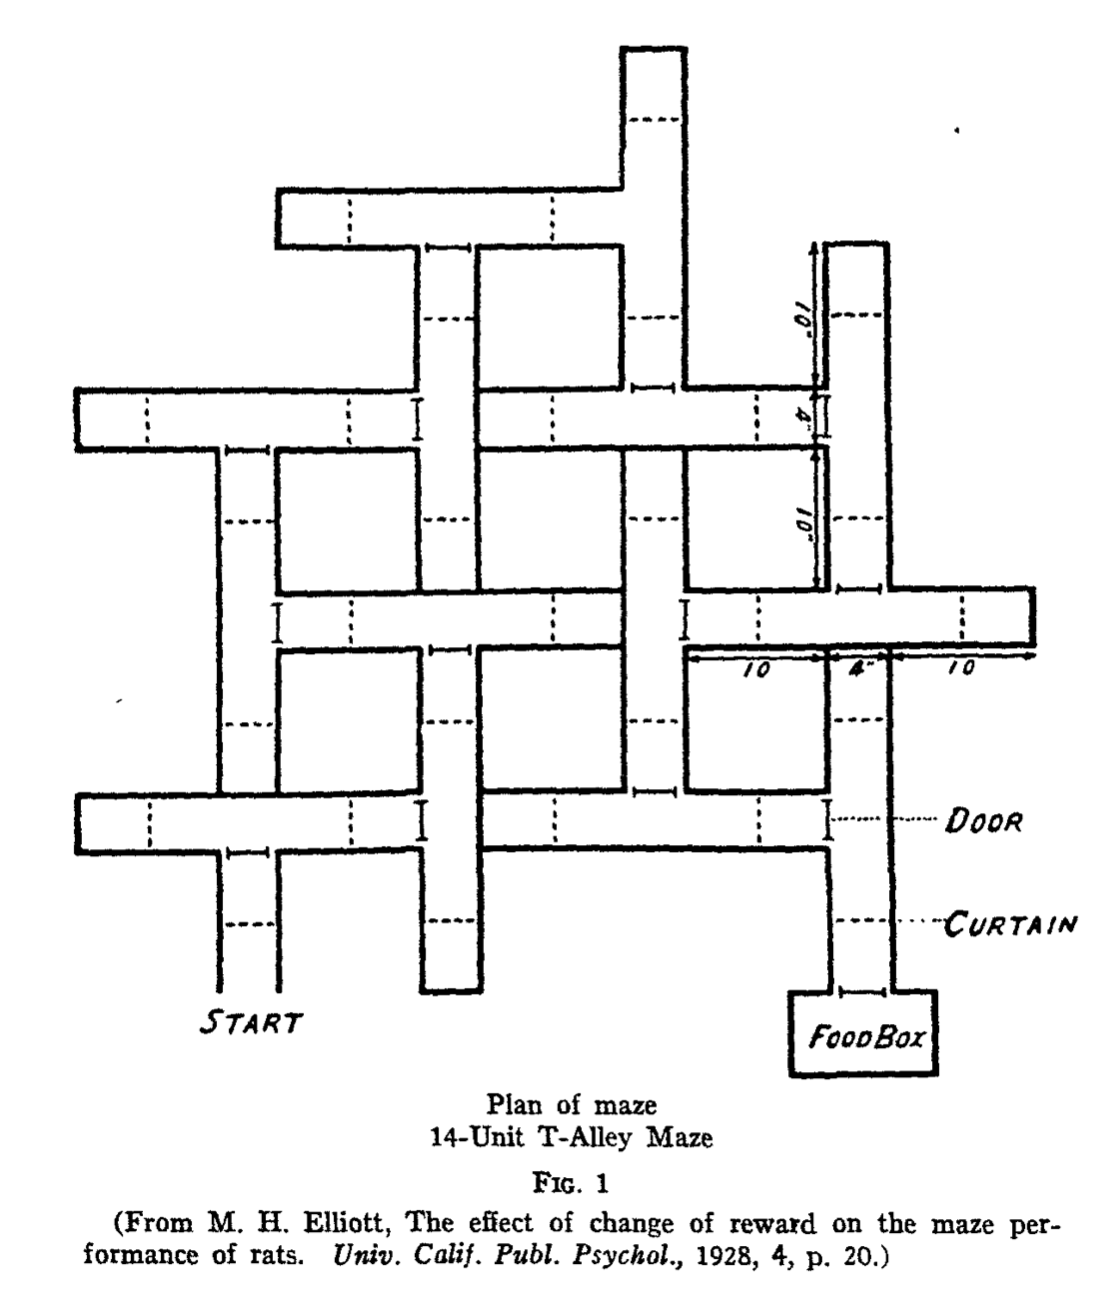
\includegraphics[width=1\linewidth]{imgs/Tolman_AlleyMaze}

\end{floatrightbox50}

Tolman argued that behaviors were obviously goal-driven and should be described in terms of goals and purposes. To support this argument, he showed that maze running behavior could be influenced by apparent goals or motivational drives. The figure depicts one of Tolman's ``Alley Mazes''. The maze had a start point where the rat entered, and an end point where it could receive food reward. In between, the rat had to navigate the maze, which contained several corridors, doors, and curtains, and many ``blind-alleys'' leading to an empty wall. In general, rats explore the maze and eventually find the food reward. The behavior of the rat can be measured in different ways, such as the total amount of time taken to succesfully navigate the maze. In the following experiment, Tolman measured the number of errors an animal made during navigation. An error is counted whenever the rat enters a blind-alley entrance.

\begin{floatrightbox50}
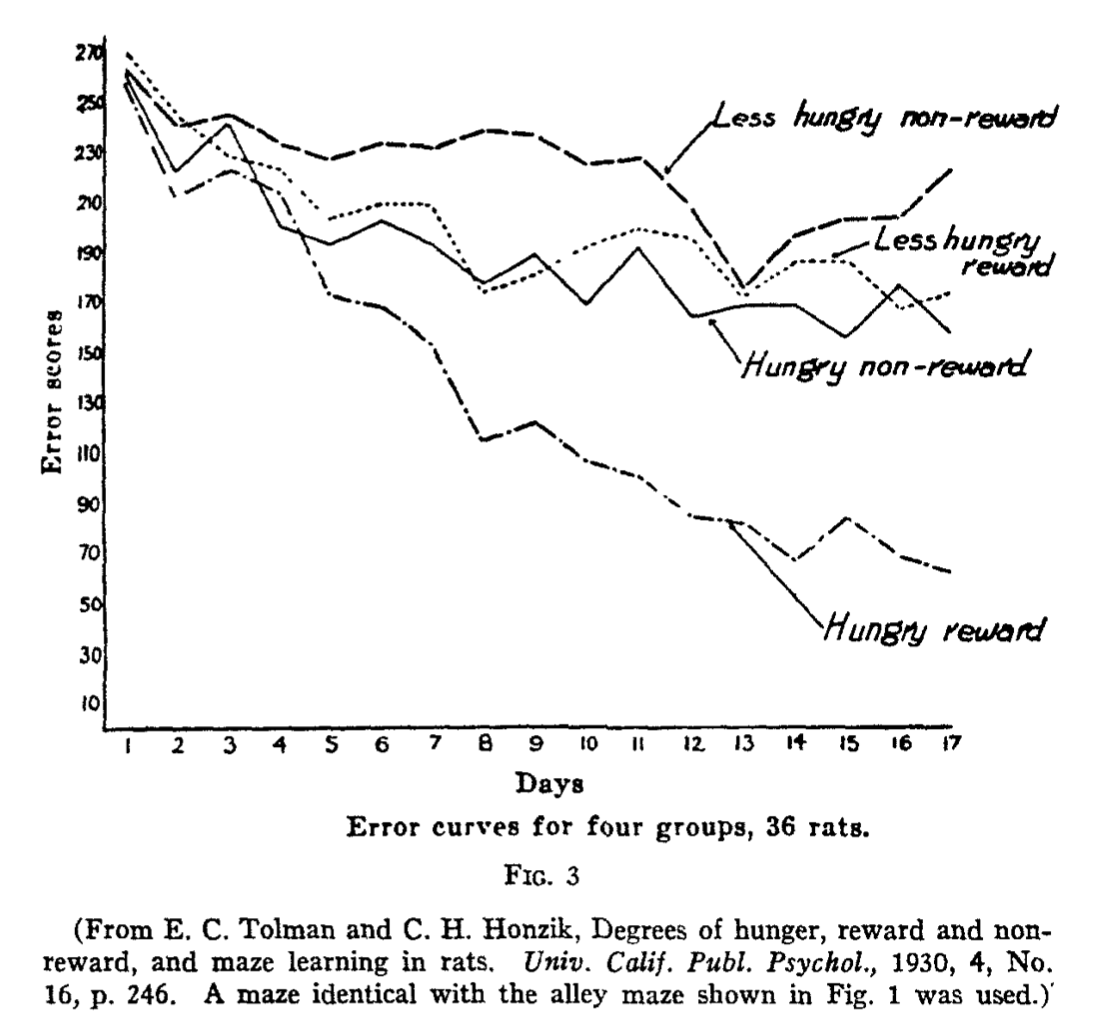
\includegraphics[width=1\linewidth]{imgs/Tolman_hunger}

\end{floatrightbox50}

In one experiment,\footnote{\protect\hyperlink{ref-tolmanDegreesHungerReward1930}{Tolman, Edward Chace, \& Honzik, C. H. (1930). Degrees of hunger, reward and non-reward, and maze learning in rats. \emph{University of California Publications in Psychology}}.} Tolman manipulated level of hunger and amount of reward. Rats ran the maze when they were either very hungry or not very hungry. Additionally, for both groups, food was either given as a reward at the end of the maze, or food was not given. The results of the experiment are shown in the figure, plotting error scores. Note also, that the experiment was conducted over many days.

In general, all groups of rats showed fewer errors across the days of the experiment (on day one, the lines started with a high number of errors, and trend downward over days to a lower number of errors). This means that the rats made fewer wrong turns as they gained experience with navigating the maze over days.

More specifically, the hunger and reward manipulations clearly influenced the number of errors that rats made over days. And, Tolman interpreted the data as consistent with the goal-driven or purposive behavior. The error scores for the ``hungry reward'' group showed the largest decreases over days compared to the other groups. According to Tolman, these rats were driven by hunger and motivated by the reward they would receive at the end. Over days, they apparently learned how to navigate the maze in an efficient manner, to get the food as quickly as possible, and without making wrong turns.

By comparison, the ``Hungry non-reward'' rats showed a decrease in errors across days, but the decrease was not as large as the first group. These rats were driven by hunger, but they were not as motivated to get to the end of the maze because there was no food at the end. Similarly, both ``less hungry'' groups showed small decreases in number of errors over days. This was consistent with having little drive to search for food in an efficient manner.

\hypertarget{cognitive-behavior}{%
\subsubsection{Cognitive Behavior}\label{cognitive-behavior}}

Tolman also argued that behavior should be described in terms of cognitive acts. He used choice and discrimination behavior in rats as evidence. The form of the argument was to first to demonstrate that a rat could distinguish between two option (discrimination), and then show that the rat's behavior showed a preference (choice) toward one of the options. This kind of behavior was characterized as being cognitive because it implied a process of considering costs and benefits of different options, and making choices to take actions that would help the animal achieve its goals.

\begin{floatrightbox50}
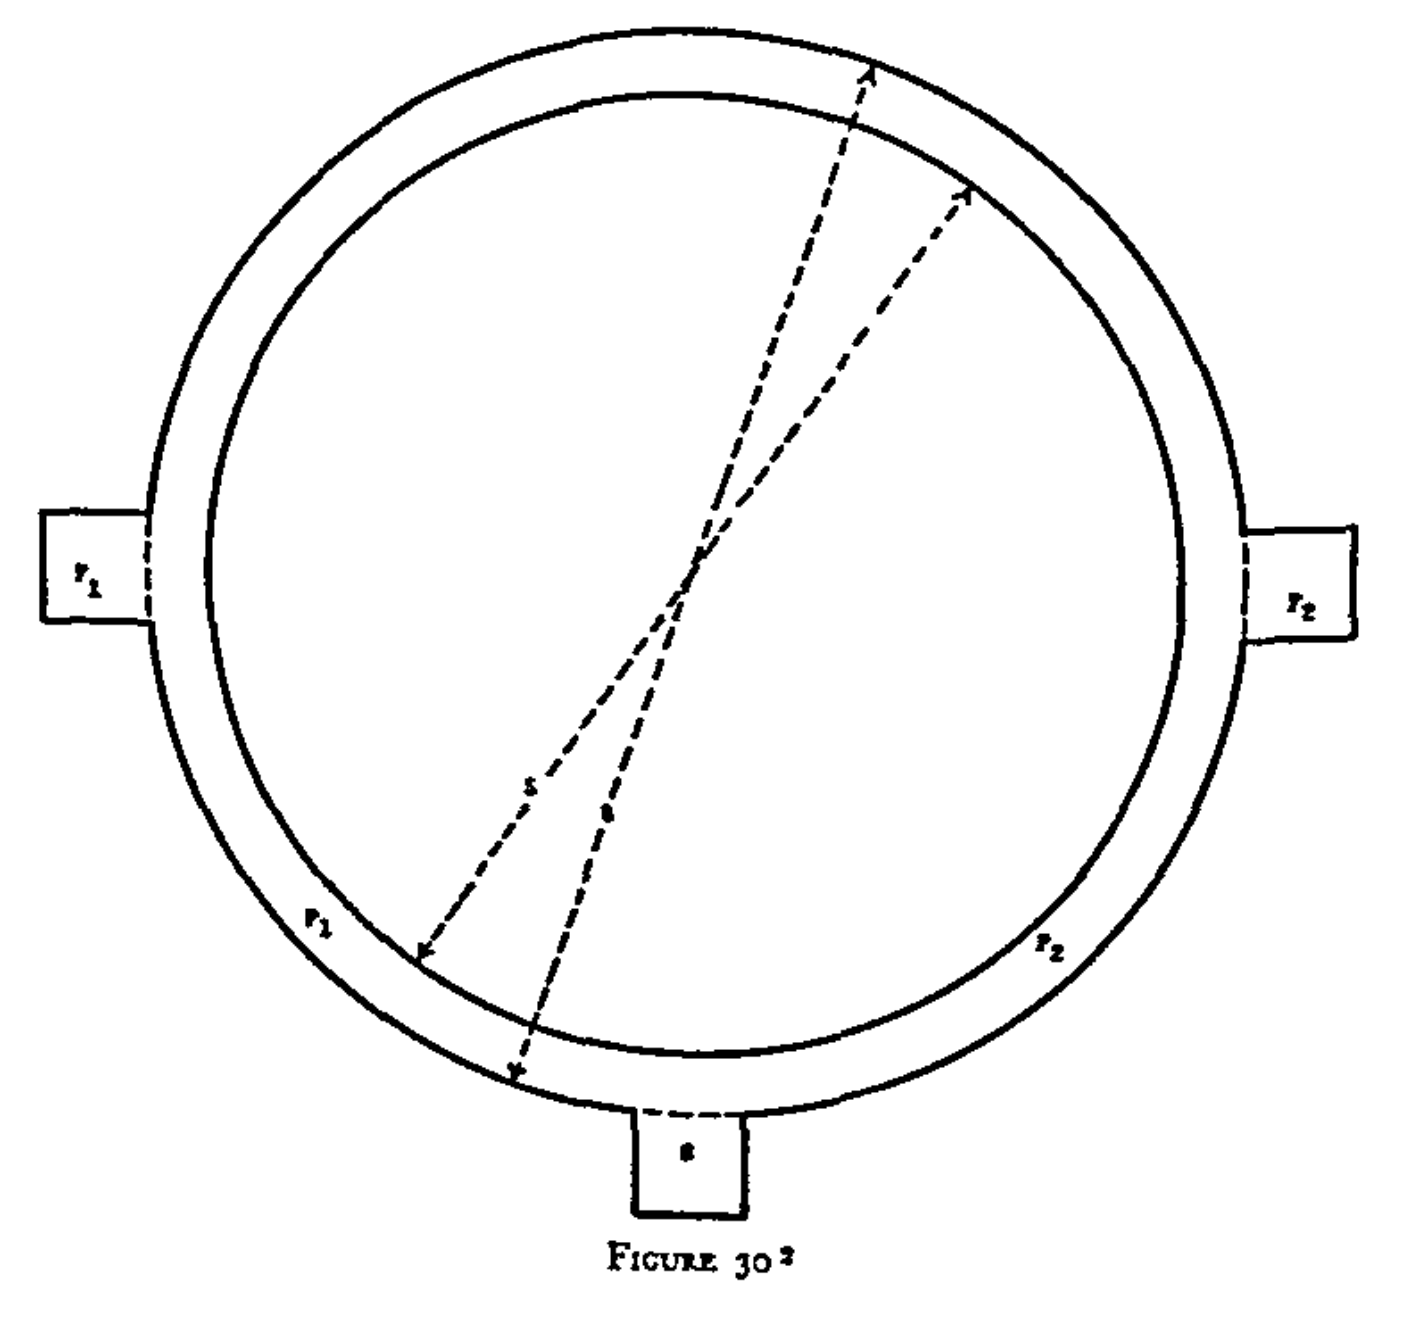
\includegraphics[width=1\linewidth]{imgs/Tolman_DistanceMaze}

\end{floatrightbox50}

Tolman credits De Camp\footnote{\protect\hyperlink{ref-decampRelativeDistanceFactor1920}{De Camp, J. E. (1920). Relative distance as a factor in the white rat's selection of a path. \emph{Psychobiology}, \emph{2}(3), 245. \url{https://doi.org/bcx2m3}}.} with connecting the results of a distance discrimination experiment to the argument that behavior should be described with cognitive features. The figure shows De Camp's circular maze. The rat entered the maze at the bottom starting point. The maze had two rooms on the left and right of the circle that could contain food. In the first phase, the right room was blocked, and food could be found in the left room. The rat's could either go the short way (turn left), or the long-way, (turn right and go around the circle). De Camp showed that with practice, rat's showed a preference for the shortest path. In a second, phase, the left room was blocked, and the right room contained the food. Again, after practice, the rat's showed a preference to turn right and take the shortest path to the food. This behavior was aptly described as cognitive, because the rats appeared to be weighing the option to go the long or short way, and choosing the shortest way to achieve their goal.

\begin{floatrightbox50}
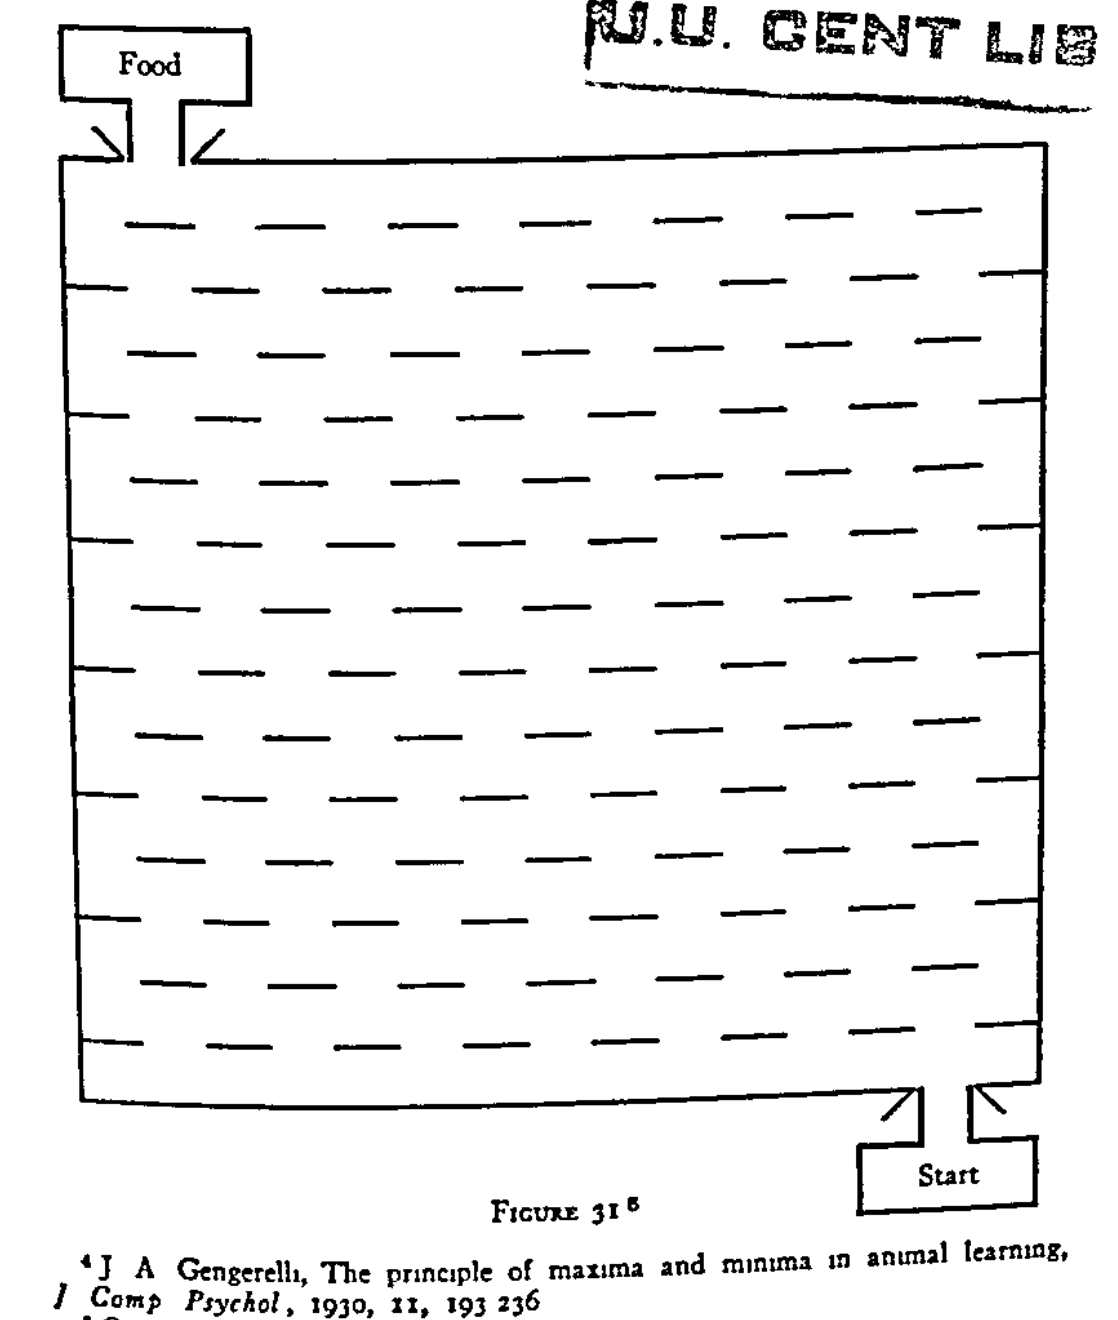
\includegraphics[width=1\linewidth]{imgs/Tolman_Minima}

\end{floatrightbox50}

Tolman points to another interesting experiment by Gengerelli,\footnote{\protect\hyperlink{ref-gengerelliPrincipleMaximaMinima1930}{Gengerelli, J. A. (1930). The principle of maxima and minima in animal learning. \emph{Journal of Comparative Psychology}, \emph{11}(2), 193. \url{https://doi.org/cfbrfs}}.} showing that rats can learn to take the shortest or most efficient path through a maze. The figure shows Gengerelli's maze, which looks kind of like a \href{https://en.wikipedia.org/wiki/Bean_machine}{bean machine}. The maze included numerous choice points where a rat could decide to turn left or right and take an open pathway or not. For example, imagine how many ways you could solve the maze with by drawing a line from the start to the finish. There are many ways, and some are longer than others. Gengerelli showed that, given multiple attempts, rats will begin taking shorter paths to get the food reward at the end.

\begin{floatrightbox50}
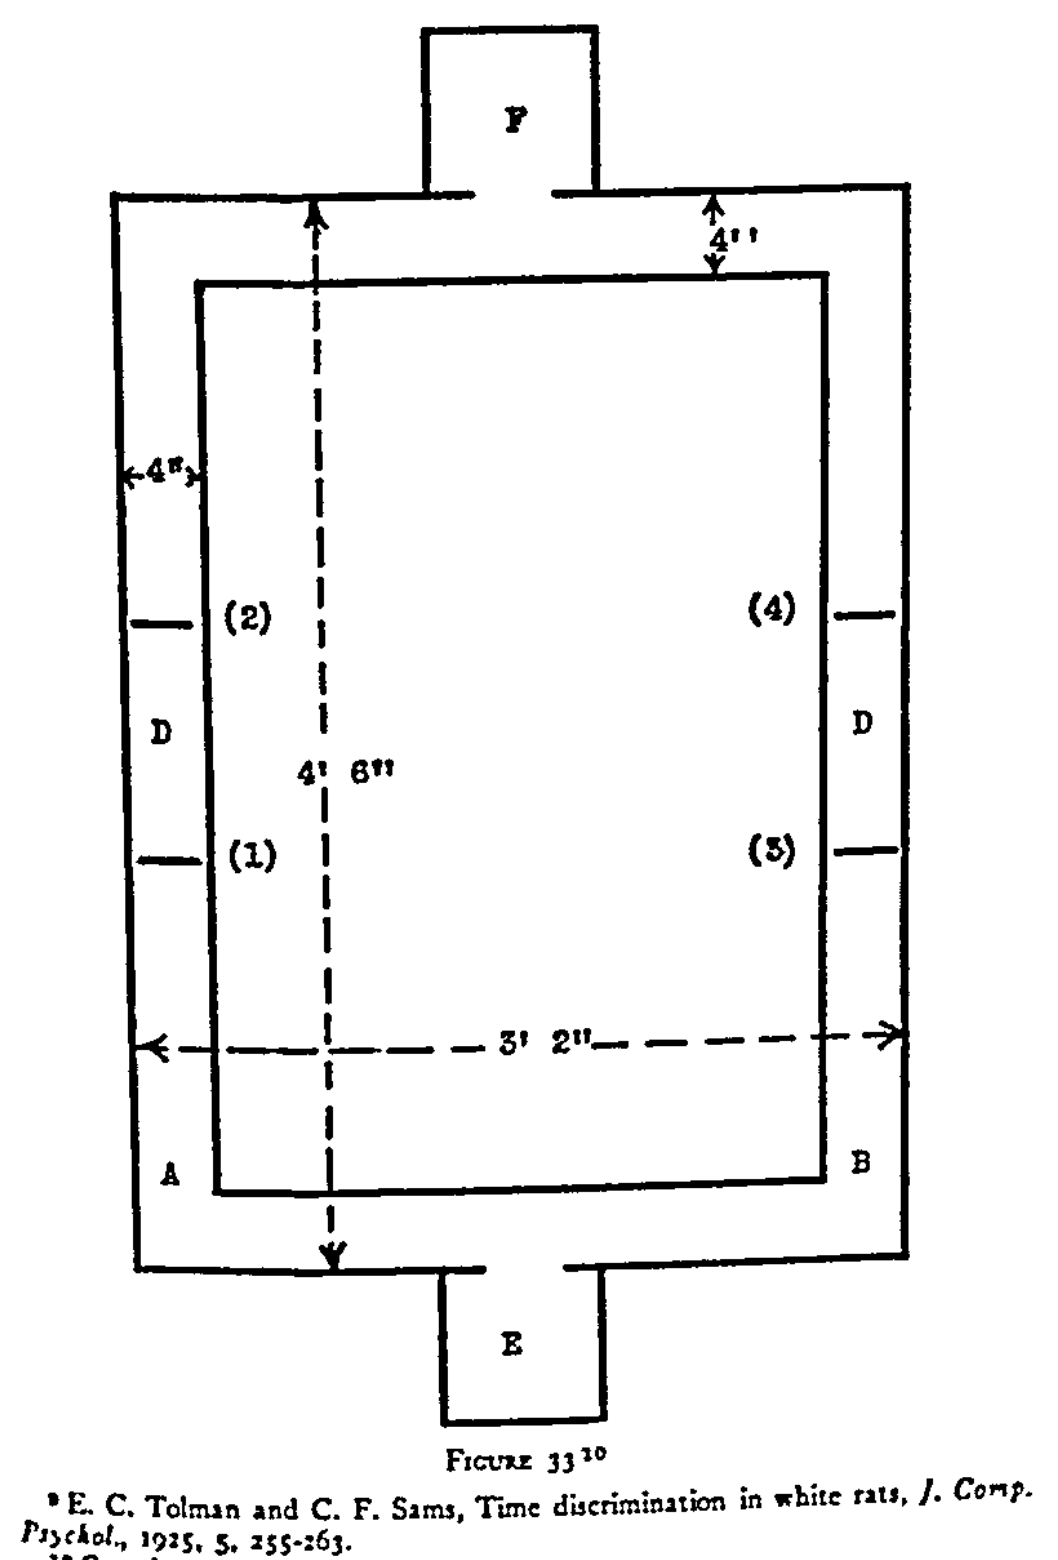
\includegraphics[width=1\linewidth]{imgs/Tolman_Temporal}

\end{floatrightbox50}

As a last example, Tolman\footnote{\protect\hyperlink{ref-samsTimeDiscriminationWhite1925}{Sams, C. F., \& Tolman, E. C. (1925). Time discrimination in white rats. \emph{Journal of Comparative Psychology}, \emph{5}(3), 255. \url{https://doi.org/bzfxwr}}.} showed that rats were capable of temporal discrimination, and appear to make choices while navigating a maze that reduce the amount of time taken to get a food reward. Tolman's temporal discrimination maze is shown in the figure. Rats started at the entrance (E), and attempted to find the food in the room on the other side (F). However, when the rats took the A corridor to the left, or the B corridor to the right, they were detained for different amounts of time in the ``detention'' rooms (D) on both sides of the maze. For example, rats would be detained for one to two minutes on the left side, or three to four minutes on the right side. After the first phase were rats experienced the delays, they were allowed to navigate the maze without being detained. The rat's showed a preference to take the route associated with the shortest temporal delay.

\hypertarget{tolmans-inheritance-project-a-rat-model-of-eugenics}{%
\subsection{Tolman's inheritance project: A rat model of eugenics}\label{tolmans-inheritance-project-a-rat-model-of-eugenics}}

Animals like rats have been used in research for many purposes. The animal may be an object of the research in its own right, or used as a model example to investigate something else, or both. For example, rats are commonly used as models for human disorders such as eating disorders and schizophrenia. One goal of research using animal models of disorders is to develop cures for the disorder in rats that could generalize to humans.

Tolman conducted animal research using rats that had elements of both styles of research. He was interested in the behavior of rats as an object of study in its own right, but also as a model in at least two respects. First, Tolman was interested in using rats as model for building a descriptive science of behavior that could be generalized to other animals. In this first respect, Tolman used his maze-running experiments to argue in favor of expanding the terms in the descriptive science of behaviorism--specifically, behaviorism should include terms for describing the purposive and cognitive aspects of behaviors. Second, Tolman initiated another line of maze-running experiments that I will describe as Tolmans' rat model of eugenics.

One aim of Galton's eugenics was to measure differences in eugenically desired traits (like intelligence), and then selectively breed humans to increase those traits (assuming they had a genetic basis) over time. Tolman and his student Robert Tryon attempted something similar in rats,\footnote{For a review see, \protect\hyperlink{ref-innisTolmanTryonEarly1992}{Innis, N. K. (1992). Tolman and {Tryon}: {Early} research on the inheritance of the ability to learn. \emph{American Psychologist}, \emph{47}(2), 190. \url{https://doi.org/cmbsqr}}.} they selectively bred rats for maze-running ability over generations. On the one hand, these experiments could be described without the term eugenics, and instead described as experiments on the genetic bases of maze-running behavior in rats. On the other hand, the connection to eugenics is clear enough, and existed before Tolman. For example, early comparative psychologists Edward Thorndike and Robert Yerkes were prominent eugenicists; and Thorndike described his puzzle box research as a preliminary step toward measuring individual differences in animal intelligence.

Like Thorndike, Tryon analogized the maze-running procedure as a tool to measure individual differences in rat intelligence. Measures of time and efficiency in navigating the maze were used as proxies for rat intelligence, and not surprisingly, there were reliable individual differences in rat maze-running performance.\footnote{\protect\hyperlink{ref-tryonIndividualDifferences1942}{Tryon, Robert C. (1942). \emph{Individual differences.} \url{https://doi.org/bs44gx}}.} Tolman first attempted a breeding program to create ``bright'' versus ``dull'' strains of maze-running rats.\footnote{\protect\hyperlink{ref-tolmanInheritanceMazelearningAbility1924}{Tolman, EDWARD CHACE. (1924). The inheritance of maze-learning ability in rats. \emph{Journal of Comparative Psychology}, \emph{4}(1), 1. \url{https://doi.org/d737hx}}.} In this work, Tolman exposed rats to a maze and measured individual differences in maze-running efficiency. He then bred ``bright'' rats together, and separately bred ``dull'' rats together. He did this over two generations, so there was a parent generation, an \(F_1\) generation and an \(F_2\) generation. Tolman reported that selective breeding did show differences in maze performance in the first generation, but not in the second generation. His student Tryon repeated a selective breeding experiment over 11 years and many more generations and found similar results.\footnote{\protect\hyperlink{ref-tryonGeneticDifferencesMaze1940}{Tryon, Robert Choate. (1940). Genetic differences in maze learning ability in rats. \emph{Yearbook of the National Society for the Study of Education}}.}

\hypertarget{cognitive-maps-in-rats-and-men}{%
\subsection{Cognitive maps in rats and men}\label{cognitive-maps-in-rats-and-men}}

To wrap up our discussion of Tolman, I will point quickly at his 1948 paper in Psychological Review called ``Cognitive maps in rats and men'' {[}Edward C. Tolman\footnote{\protect\hyperlink{ref-tolmanCognitiveMapsRats1948}{1948}.}. This paper reflects Tolman's thinking 16 years later. He reviews maze-running research up to 1948, and appears to have shifted away from his descriptive stance on cognitive aspects of behavior. In 1932, Tolman was careful to argue that his use of words like ``cognitive'' or ``purpose'' were meant only as descriptive terms of behavior, and they were not intended to imply the existence of internal mentalistic-type processing. In 1948, Tolman expresses a much more cognitive interpretation, where ``cognitive'' is used to refer to a process, or intervening set of operations between the stimulus and response, that is fundamental to the behavior. In particular, Tolman argues that rats learn cognitive maps of the mazes they are running. This is the idea that the rat has some kind of internal map-like representation of the maze that they use to inform their choices while running the maze. One line of evidence supporting Tolman's position came from experiments on latent-learning.

\hypertarget{latent-learning-as-evidence-for-cognitive-maps}{%
\subsubsection{Latent-learning as evidence for cognitive maps}\label{latent-learning-as-evidence-for-cognitive-maps}}

\begin{floatrightbox25}
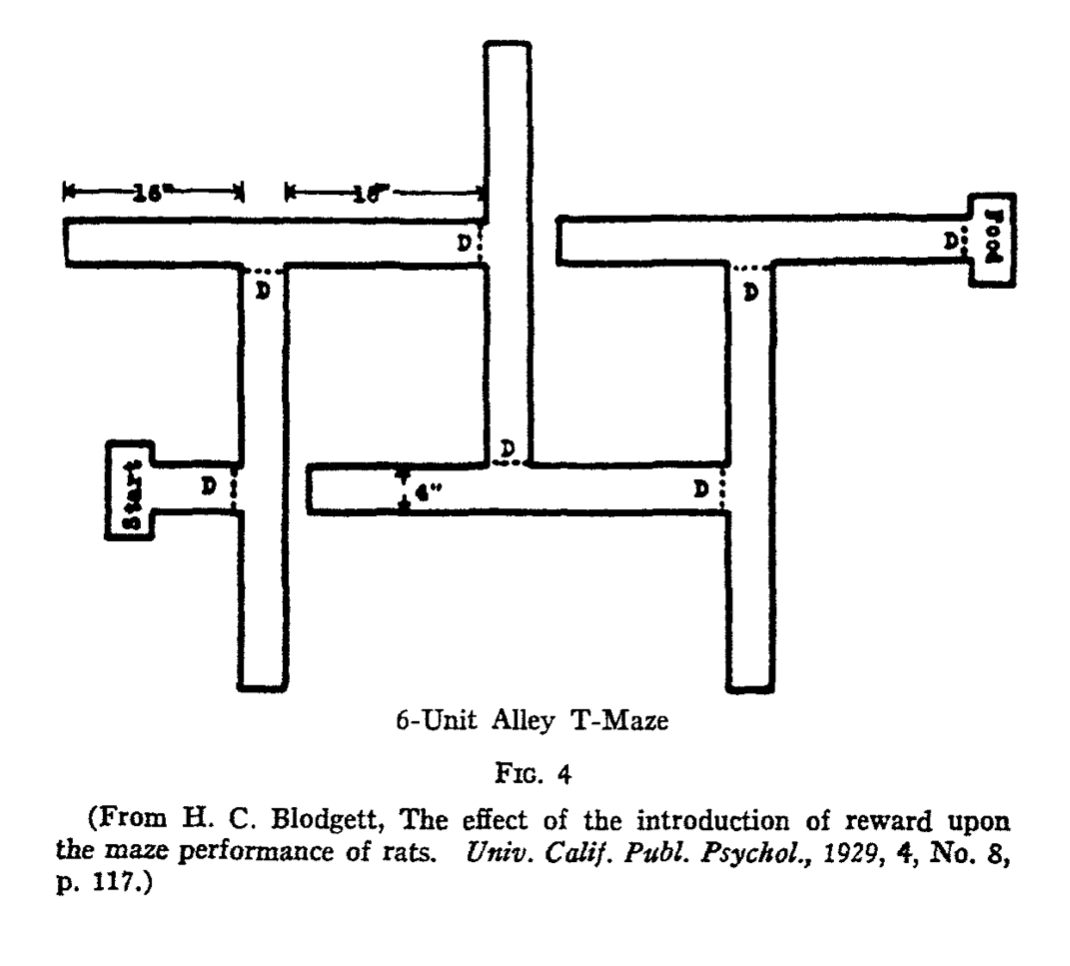
\includegraphics[width=1\linewidth]{imgs/Tolman_latentmap}

\end{floatrightbox25}

Tolman credits Bodgett\footnote{\protect\hyperlink{ref-blodgettEffectIntroductionReward1929}{Blodgett, H. C. (1929). The effect of the introduction of reward upon the maze performance of rats. \emph{University of California Publications in Psychology}}.} with introducing the concept of latent learning to maze-running experiments. Latent learning refers to something an animal apparently learned without expressing the learning in performance. Bodgett demonstrated latent learning by giving three groups of rats different kinds of experience with running the maze.

\begin{floatrightbox50}
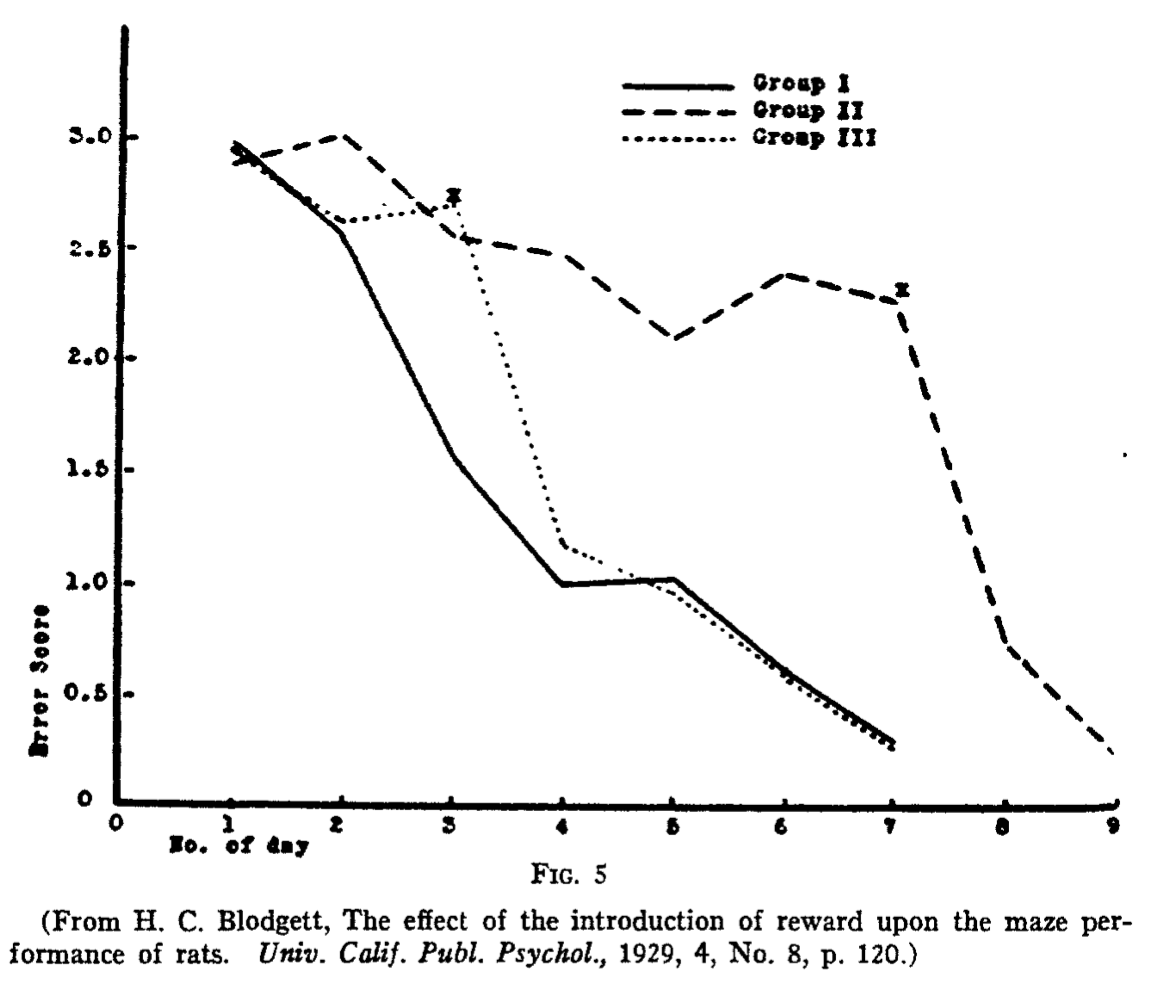
\includegraphics[width=1\linewidth]{imgs/Tolman_latentresults}

\end{floatrightbox50}

Group I (represented by the solid line) always received food reward in the chamber at the end of the maze. The results show that group made fewer and fewer errors across days. Group II (the dotted line) did not get food reward at the end maze until day three. Day three is marked with an X. Up to day three, group II did not show a great reduction in number of errors, but after day three they did show a very large reduction in errors. Group III (the dashed line) did not get food reward at the end of the maze unitl day 7. That group did not show major decreases in errors until after day, when they showed a dramatic decrease in errors. Here is a quote from Tolman showing how he connected these findings with the notion of a cognitive map:

\begin{quote}
``It will be observed that the experimental groups as long as they were not finding food did not appear to learn much. (Their error curves did not drop.) But on the days immediately succeeding their first finding of the food their error curves did drop astoundingly. It appeared, in short, that during the non-rewarded trials these animals had been learning much more than they had exhibited. This learning, which did not manifest itself until after the food had been introduced, Blodgett called''latent learning.'' Interpreting these results anthopomorphically, we would say that as long as the animals were not getting any food at the end of the maze continued to take their time in going through it -- they continued to enter many blinds. Once, however, they knew they were to get food, they demonstrated that during these preceding non-rewarded trials they had learned where many of the blinds were. They had been building up a `map,' and could utilize the latter as they were motivated to do so''.
\end{quote}

\hypertarget{implications-for-society}{%
\subsubsection{Implications for society}\label{implications-for-society}}

Tolman's earlier work was very much in the tradition of positivism we have been discussing. One aspect of that tradition involved developing descriptive systems for natural phenomena under investigation. In his behaviorism days, Tolman argued that cognitive terminology should be used to describe behaviors, but not to imply any cognitive operations. Later on, he shows an inclination toward cognitivism, which would involve legitimizing so-called cognitive processes as a topic of scientific inquiry. In Tolman's case, he suggested that cognitive maps were entities or operations, and not just descriptors, that should be considered as units of study.

Scientific utopianism is another tradition of positivism. For example, Watson's vision of behaviorism included grandiose claims about how society would be improved by behaviorism. Tolman was more circumscribed than Watson, but in the positivist tradition chose to devote the final pages of his psychological review paper to speculate on how his concept of cognitive maps in rats could be generalized to humans for the benefit of society. Whatever his prior views were on eugenics, and considering that he was writing in 1948 after eugenics was in decline following the atrocities of world war II, his recommendations for improving society were much more inclusive by comparison. He likened navigating a maze to living in the world, and suggested that people needed to acquire ``comprehensive'' and rational maps of the world. People for too long had acquired narrow-minded maps and pursued courses of action that could lead to violent conflict. Instead, Tolman wrote:

\begin{quote}
``the child-trainers and the world-planners of the future can only, if at all, bring about the presence of the required rationality (i.e., comprehensive maps) if they see to it that nobody's children are too over-motivated or too frustrated. Only then can these children learn to look before and after, learn to see that there are often round-about and safer paths to their quite proper goals--learn that is to realize that the well-beings of {[}all people{]} are mutually interdependent''.
\end{quote}

\hypertarget{hulls-mathematical-behaviorism}{%
\section{Hull's mathematical behaviorism}\label{hulls-mathematical-behaviorism}}

\begin{floatright25}
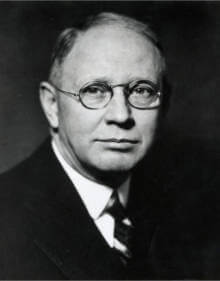
\includegraphics[width=1\linewidth]{imgs/clark-l-hull}

\end{floatright25}

\href{https://en.wikipedia.org/wiki/Clark_L._Hull}{Clark L. Hull's} (1884-1952) flavor of behaviorism was again in the positivist tradition, but more focused on using math to specify functional relationships between units of behavior. In the positive tradition, a scientific theory is tentative and pragmatic. It is useful if it works for purposes of manipulation and control. Mathematical formulations are not strictly necessary, but they are often useful in describing functional relationships for purposes of prediction.

\begin{floatrightbox50}
Hull also worked during the eugenics era in American psycholgoy. He was recruited to Yale in 1929 by then president \href{https://en.wikipedia.org/wiki/James_Rowland_Angell}{James R. Angell}, who was previously a psychologist running a nationally recognized eugenics laboratory. Hull was recruited into Yale's burgeoning new enterprise, the Institute for Human Relations (IHR). Hull was hired as a mental tester, and among his first grant applications to the institute was a program of eugenics (see also the role of eugenics in the early Yale psychology department\footnote{\protect\hyperlink{ref-doyleMeasuringProblemsHuman2014}{Doyle, J. (2014). \emph{Measuring "{Problems} of {Human Behavior}": {The Eugenic Origins} of {Yale}'s {Institute} of {Psychology}, 1921-1929}. 70}.} and more on Hull's influence in the IHR).\footnote{\protect\hyperlink{ref-morawskiOrganizingKnowledgeBehavior1986}{Morawski, J. G. (1986). Organizing {Knowledge} and {Behavior} at {Yale}'s {Institute} of {Human Relations}. \emph{Isis}, \emph{77}(2), 219--242. \url{https://doi.org/bh5f9m}}.}

\end{floatrightbox50}

To contrast with Hull, Watson did not attempt to formulate any precise mathematical theory linking the terms in his system. Watson used simple terms like stimulus and response, and put them in a mock ``algebra''. For example, one could state ``S -\textgreater{} R?'', and solve the equation by experimentally determining what responses \(R\) were caused by some stimuli \(S\).

Hull's work is one example of attempting both to specify descriptive terms for a science of behavior (terms like stimulus and response, and also terms for drives and motivations), and to use math to describe supposedly lawful patterns linking terms in the system. There was a hope in this exercise that behavior itself was lawful. If so, behavior could be observed and fitted to the terms in the equations. Then, assuming the equation correctly described the lawful aspects of the behavior, it was supposed to predict how behavior would unfold under given circumstances specified by the equation.

Here is an example \footnote{taken from wikipedia} of Hull's formula for behavior described in ``Principles of Behavior'':\footnote{\protect\hyperlink{ref-hullPrinciplesBehaviorIntroduction1943}{Hull, C. L. (1943). \emph{Principles of behavior: {An} introduction to behavior theory.}}}

\(_SE_R = _SH_R × D × V × K\)

Where:

\begin{itemize}
\item
  \(_SE_R\) is an excitatory potential (likelihood that the organism would produce response r to stimulus s),
\item
  \(_SH_R\) is the habit strength (derived from previous conditioning trials),
\item
  \(D\) is drive strength (determined by, e.g., the hours of deprivation of food, water, etc.),
\item
  \(V\) is stimulus intensity dynamism (some stimuli will have greater influences than others, such as the lighting of a situation)
\item
  \(K\) is incentive (how appealing the result of the action is).
\end{itemize}

Hull's mathematical theory did not succeed in explaining and predicting behavior in any general sense. But, it did succeed in inspiring other psychologists to adopt mathematical formulations to describe psychological processes. We will return to the topic of mathematical and computational models in a later chapter, which are now a routine part of theorizing in cognitive psychology.

\hypertarget{skinners-radical-behaviorism}{%
\section{Skinner's ``Radical'' Behaviorism}\label{skinners-radical-behaviorism}}

\begin{floatright25}
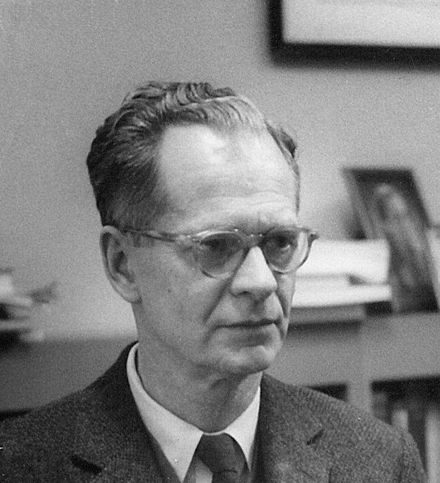
\includegraphics[width=1\linewidth]{imgs/bf_skinner}

\end{floatright25}

\href{https://en.wikipedia.org/wiki/B._F._Skinner}{Burrhus F. Skinner} (1904--1990) received his Ph.D.~at Harvard in 1931, where he spent the majority of his later academic career. Skinner had a profound impact on psychology and cognitive psychology both in terms of his ideas and the number of graduate students he mentored that would continue to shape the field. Skinner is often associated with the term ``radical behaviorism'', and although he did refer to his work this way on occasion, the term was in use more broadly to describe behaviorist ideas as ``radical'' in relation to other ideas in psychology.\footnote{For more see, \protect\hyperlink{ref-schneiderHistoryTermRadical1987}{Schneider \& Morris, 1987}.}

Skinner is well-known for introducing the method of operant conditioning, which he distinguishes from classical conditioning shown by Pavlov. Skinner uses the terms type R learning for operant conditioning, and type S learning for Pavlovian conditioning. In this section we will examine the method of operant conditioning, a few major findings from operant conditioning research, and Skinner's attempt to create a descriptive system of behavior in the positivist tradition.

\hypertarget{operant-conditioning}{%
\subsection{Operant Conditioning}\label{operant-conditioning}}

In type S Learning, an S-R relationship is already established before conditioning begins. For example, the unconditioned stimulus (e.g., food) elicits a response (e.g., salivating) before any acquisition phase. Through the process of pairing a neutral stimulus (e.g., a tone) with the unconditioned stimulus, the neutral stimulus can acquire the ability to trigger the response on its own.

In type R learning, S-R relationships may not exist or may not be known prior to conditioning. Skinner pointed out that many responses in animal behavior occur with different frequencies, without being triggered by any obvious stimulus in the environment. He termed these behaviors operants. For example, a rat placed in a box will show many behaviors (e.g., walking, licking, scratching, sniffing, an so on). These individual behaviors will repeat over time, and some behaviors will occur more frequently than others. All of these behaviors could be considered operants, which are the repertoire of behaviors that an animal can perform. Before type R learning, the operant behavior could be said to have some probability of occurring on its own. The goal of type R learning was to gain control over the operant behavior, such that the occurrence and frequency of the behavior could be made predictable.

Operant conditioning is commonly used to train behaviors in animals such that they perform a desired action in response to a stimulus, or perform the action in a predictable manner in a given situation. For example, I think I accidentally conditioned our two cats Coco-Max, and Mr.~Ernie Cactus, using type R learning. Both cats show the ``operant behavior'' of sometimes running into the living room. They do this at least a few times every day, and they did this before their crinkly bag of cat snacks were kept in a drawer in the living room. When I give the cats snacks, I take the bag out, open it up, and hand out the snacks. The bag makes a distinct crinkly noise, just like the sound of the treats when the bag is shook. The cats have been given many snacks in the living room\ldots and we can consider this something like an operant conditioning procedure. Now, the behavior of cats running into the living room is very much under stimulus control. It appears that my cats have a keen sense of hearing, whenever they hear the drawer move a little bit, or the bag crinkle, or shake, they come galloping into the living room from any corner of the apartment.

\hypertarget{lever-pressing-in-the-skinner-box}{%
\subsubsection{Lever pressing in the Skinner box}\label{lever-pressing-in-the-skinner-box}}

Skinner demonstrated operant conditioning in rats using a ``Skinner-box'' and a lever-pressing device. Unlike Thorndike's puzzle boxes, where animals demonstrated learning by escaping the boxes as quickly as possible; Skinner's boxes were constructed to contain the animal and create an environment where a particular behavior could be efficiently observed and measures.

\begin{floatright50}
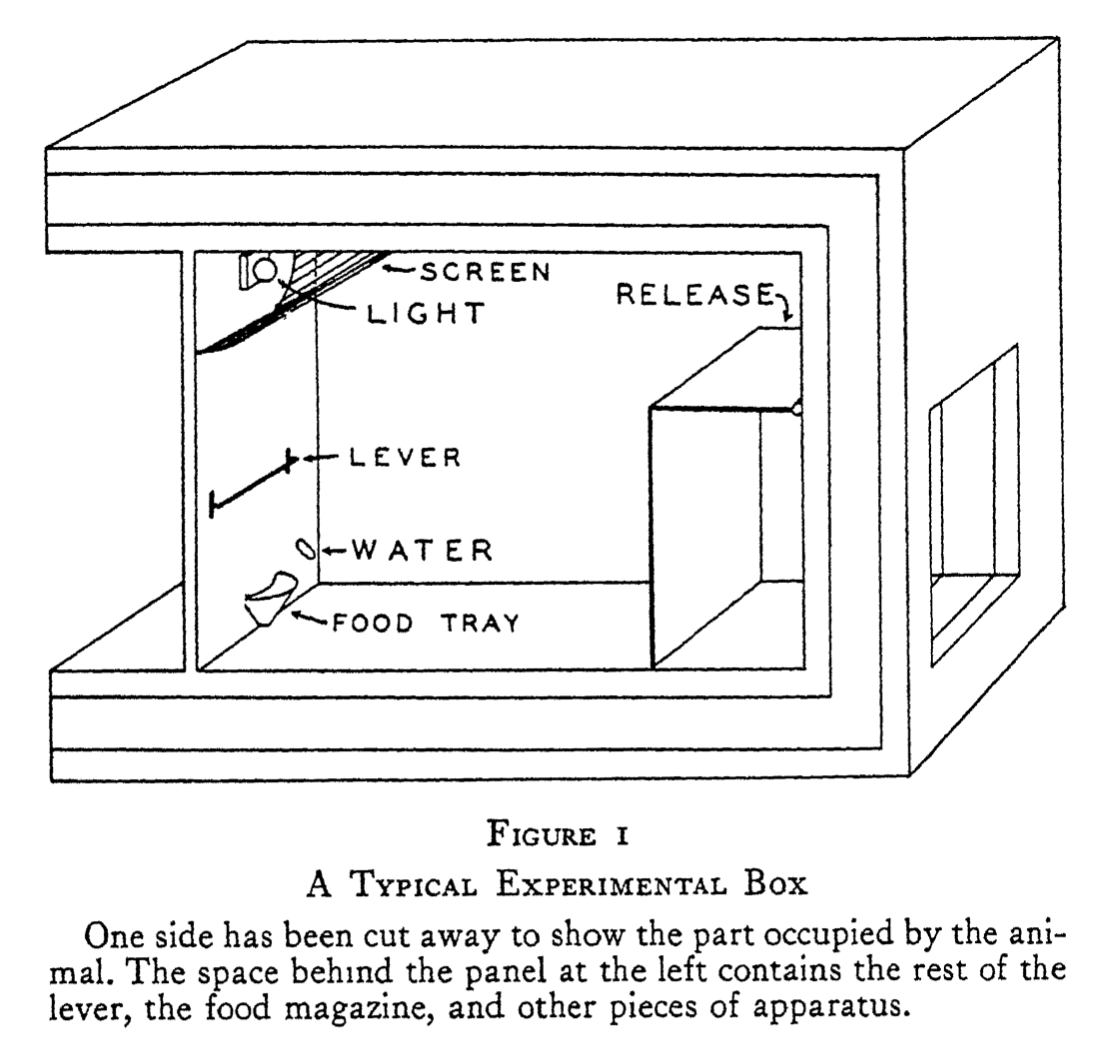
\includegraphics[width=1\linewidth]{imgs/Skinner_Box}

\end{floatright50}

The example skinner box to the right shows the box had space for a single rat to move about, and mechanisms for water and food delivery. The box also contained a lever the animal could press in order to receive food reward (subject to experimenter control). And, the box was set up to record any lever presses the animal made.

Lever-pressing is a good example of an operant behavior that occurs without any prior conditioning. For example,Skinner noted that rat's placed into his box for the first time would press the lever sometimes, even though the box was not associated with any food reward, and even though pressing the lever did not cause any food to be delivered. In other words, rats spontaneously pressed the lever sometimes. As a result, lever-pressing was a convenient operant behavior for type R conditioning.

Skinner assumed that operant behavior, like pressing a lever, could become reinforced if it was paired with a reward. For example, if the lever-pressing behavior was paired with food reward, Skinner assumed that the food would reward the animal for the behavior. This would lead to the behavior being reinforced, such that the animal would increase the lever-pressing behavior. However, in order for reinforcement to occur, the behavior had to take place and be rewarded. For example, lever-pressing would be difficult to condition if the animal didn't press the lever sometimes.

Skinner's procedure for conditioning lever-pressing was very simple. He put rats in the Skinner box ad measured how many times they pressed the lever over time without any reward. This established a baseline frequency for the spontaneous occurence of the operant behavior. Then, the lever was connected to food delivery. Whenever, the animal pressed the lever, it received a food pellet. Skinner then observed the animal and measured each of the lever-presses over time.

\begin{floatright50}
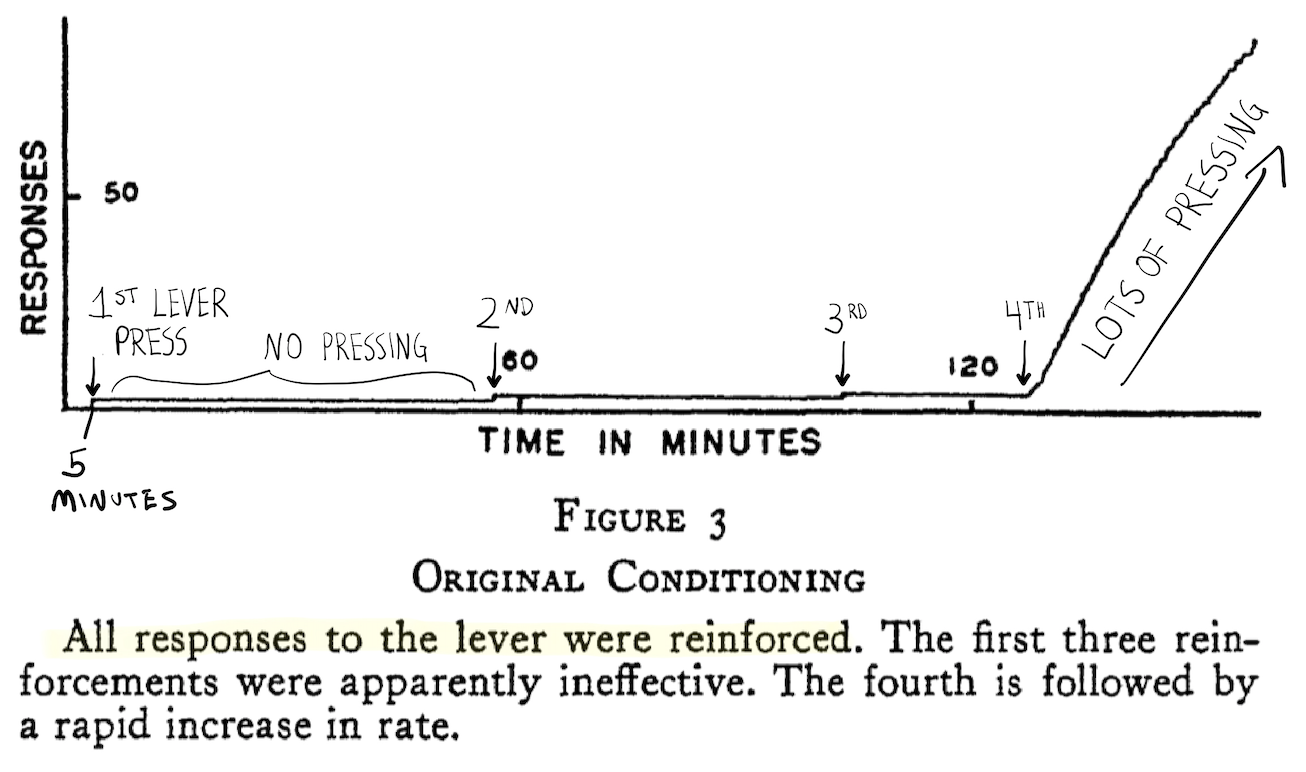
\includegraphics[width=1\linewidth]{imgs/Skinner_Results}

\end{floatright50}

The figure shows an example of Skinner's findings in a simple operant conditioning procedure. The Y axis shows the total number of lever presses, and the X axis shows time in minutes. The line represents lever-pressing behavior over time. The rat pressed lever for the first time after 5 minutes inside the box, and then received a food reward. Then it waited a long time (almost an hour) and pressed the lever a 2nd time, and then waited again and pressed a 3rd then 4th time. Look what happens after the 4th press. The line veers up, indicating the rat began pressing the lever at a much higher rate.

This is an example of operant conditioning. Prior to conditioning the lever-pressing behavior occurred spontaneously and not very often. However, in the setting of the Skinner Box, and when lever-pressing was paired with food reward, the animal began showing the lever-pressing behavior with a great deal of regularity. In this sense, as a result of the conditioning procedure, the lever-pressing behaviour is said to have come under experimental control.

\hypertarget{interpreting-a-cumulative-response-graph}{%
\subsubsection{Interpreting a cumulative response graph}\label{interpreting-a-cumulative-response-graph}}

Skinner had several reasons for choosing lever-pressing as a behavior to investigate in the laboratory. One reason was convenience. Lever-pressing was easy to measure, rat's exhibited the behavior spontaneously, and the behavior could be conditioned through ``type R'' learning. The overarching reason was to construct a descriptive theory of behavior (again in the positivist tradition), starting with lever-pressing as a very simple model of other behaviors. To appreciate these larger aims, let's take a closer look at the graphs of lever-pressing behavior over time.

Skinner usually plotted responses over time in a cumulative graph. Cumulative means that the line represents the ``accumulation'' of responses over time. In other words, at each point in time on the X axis, the vertical position of the line on the Y axis indicates the sum total number of responses occurring up to that point in time.

\begin{floatright50}
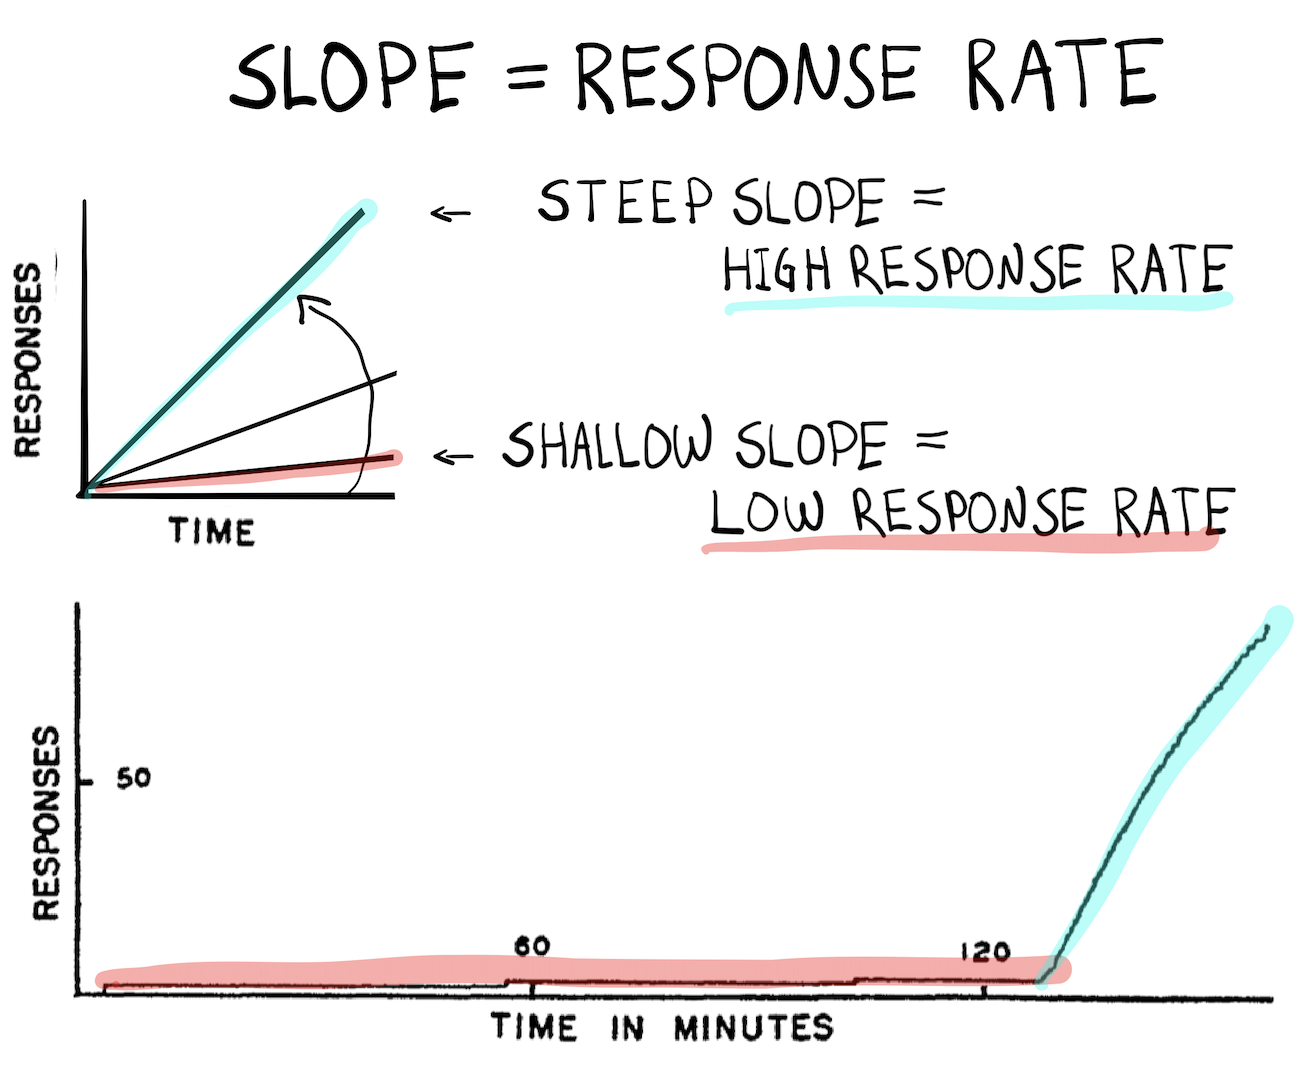
\includegraphics[width=1\linewidth]{imgs/Skinner_Slope}

\end{floatright50}

Importantly, the slope of the line in the graph has a special meaning, it represents the rate of responding. The rate of responding (or response rate) is a ratio of the number of responses divided by amount of time. For example, the first 4 responses occurred in about 120 minutes, so the response rate could be calculated as \(4/120 = .033\) (responses per minute). Notice the line in the graph up to the 4th response has a very shallow slope, this indicates a low rate of responding (e.g., only .033 responses per minute). After the fourth response, the slope of the line becomes much steeper, indicating a much higher rate of responding. By rough visual inspection of the graph, it looks like close to 100 lever-presses were made in about 30 minutes, or a response rate of \(100/30 = 3.33\) (responses per minute).

\hypertarget{reflex-strength-a-descriptive-system}{%
\subsection{Reflex strength: A descriptive system}\label{reflex-strength-a-descriptive-system}}

Skinner used lever-pressing behavior in the white rat as a convenient simple behavior that he could exhaustively study as a model system, which he intended to generalize to other behaviors and animals. His book ``The Behavior of Organisms''\footnote{\protect\hyperlink{ref-skinnerBehaviorOrganismsExperimental1938}{Skinner, B. F. (1938). \emph{The behavior of organisms: {An} experimental analysis}. {D Appleton-Century Company}}.} describes many of his experiments and findings, but also motivates and describes his positivist approach to behavior. The goal of Skinner's system was not to explain behavior, but instead to create a system for describing features and laws of behavior. If Skinner could succeed in providing a comprehensive description of how to control a simple behavior, like lever-pressing, and if other behaviors were basically like lever-pressing, then the system could be generalized to describe and control other behaviors.

We will spend a little bit more time on Skinner's system because it represents an approach to science that can lead to prediction and control of a natural phenomena (e.g., like cognition or behavior) without explaining the mechanisms of the phenomena. Skinner's descriptive approach remains very common in cognitive psychology.

\hypertarget{everyday-description}{%
\subsubsection{Everyday Description}\label{everyday-description}}

To give an example of the descriptive nature of Skinner's system, consider the figure below. The figure is a cartoon summary of how white rats typically behave in the Skinner box under different conditions.

\begin{center}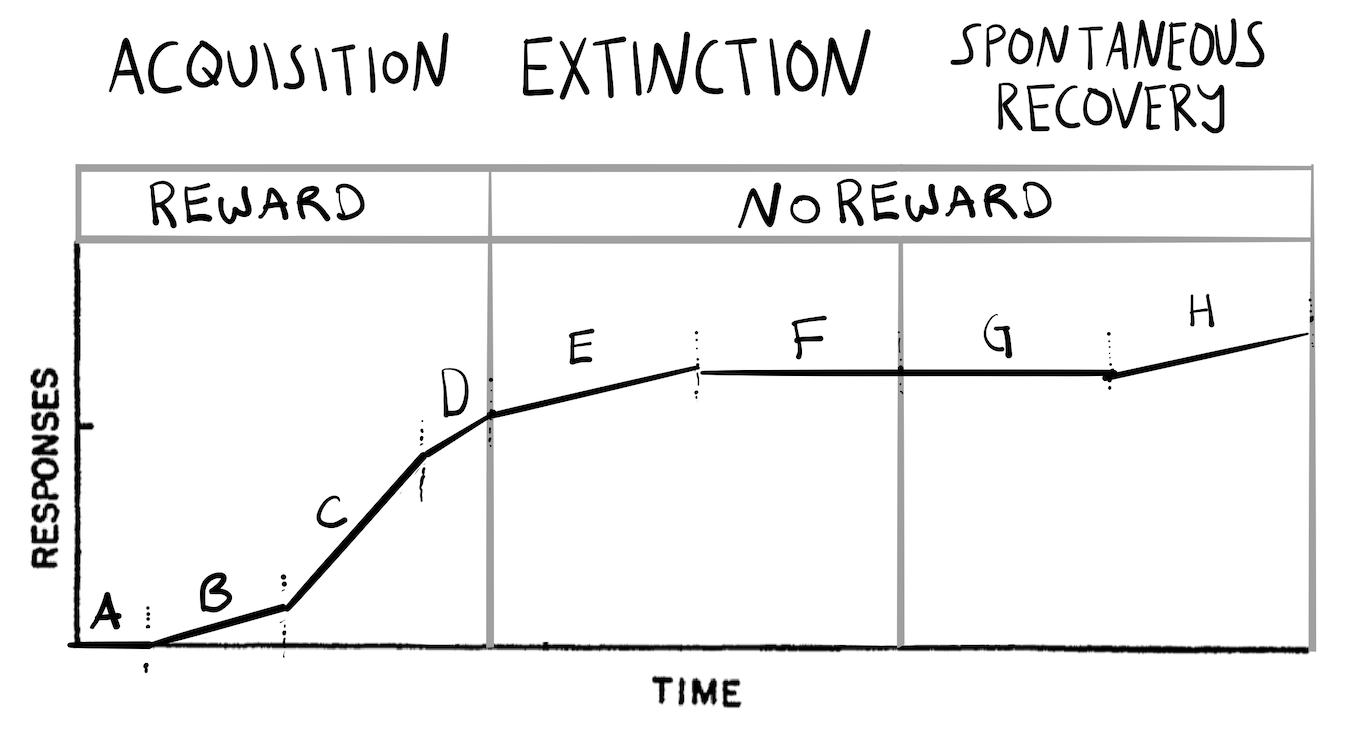
\includegraphics[width=1\linewidth]{imgs/Skinner_description} \end{center}

Notice the graph is purely descriptive in two senses. First, the line describes lever-pressing over time. Second, I have added terms to describe conditions and phases of the experiment. I also added letters to individual line segments to highlight how Skinner's system involved using abstract terms to describe what he argued were generalizable components of behavior. To contrast some ways we could describe this graph, first let me describe it using ``everyday language'', then let's use Skinner's system to describe it.

In the acquisition phase, the animal is rewarded with food every time the lever is pressed. Initially the animal doesn't respond (A); then it responds at a low rate and learns it will receive a reward (B); after the ``insight'' that the responding gives a reward the animal starts pressing the button at a high rate (C); as the animal gets many rewards it becomes less hungry, the reward is less desirable, and the rate of responding starts to decrease again (D). During the extinction phase the lever-pressing behavior no longer triggers any food-reward. Initially, the animal continues to press the lever, perhaps because it expects to get the food reward (E), but over time the animal learns that pressing the lever does not bring food, so it slows or even completely stops responding (F). Finally, what happens if you keep the animal in the box after it stopped pressing the bar? Just like in Pavlovian conditioning, it is possible to observe spontaneous recover. For example, the animal may not press the lever for a while (G), but after some time it will often start pressing the lever again (H), as if it expects food, even though it is no longer getting any.

\hypertarget{systematic-description-setting-terms-and-laws}{%
\subsubsection{Systematic Description: Setting terms and laws}\label{systematic-description-setting-terms-and-laws}}

Skinner's system involved his own set of terms and law relationships. The terms were intended as abstractions, and the laws were supposed to be empirically verified regularities in behavior. The system could be modified over time if new experiments revealed new laws, or forced revisions of old laws. And, terms in the system could be added or subtracted depending on whether they were useful to describing behavior.

Skinner used terms like \textbf{reflex} and \textbf{reflex strength}, but stripped them of their normal everyday meaning. For example, his reflex just refers to any operant behavior like lever-pressing, and is not to be mistaken with a ``real reflex''. Similarly, the strength of a reflex is an abstract quantity in the system, referring to changes in behavior over time. Reflex strength was not the magnitude of response. For example, an animal could very softly hit the lever (a weak response magnitude), but if it increased the number of times it hit the lever (while hitting it soft or hard), the reflex could be described as increasing in strength.

Other terms involved concepts like \textbf{threshold}, \textbf{latency}, \textbf{after-discharge}, which were defined by postulated laws of behavior, such as:

\begin{quote}
\textbf{The Law of Threshold} The intensity of the stimulus must reach or exceed a certain critical value (called the threshold) in order to elicit a response.
\end{quote}

\begin{quote}
\textbf{The Law of Latency} An interval of time (called the latency) elapses between the beginning of the stimulus and the beginning of the response.
\end{quote}

\begin{quote}
\textbf{The Law of the Magnitude of the Response} The magnitude of the response is a function of the intensity of the stimulus.
\end{quote}

\begin{quote}
\textbf{The Law of After-Discharge} The response may persist for some time after the cessation of the stimulus
\end{quote}

Note that the whole enterprise of proposing \href{https://en.wikipedia.org/wiki/Scientific_law}{scientific laws} for behavior was a hopeful one. Behaviorists were modeling themselves after other disciplines like physics, where many \href{https://en.wikipedia.org/wiki/Scientific_law\#Laws_of_physics}{physical laws} had been discovered. However, the behavior of animals can be highly complex and not easily captured by simple laws. To accommodate the complexity, Skinner postulates laws in a vague and provisional way. For example, in the law of after-discharge, the response \emph{may} persist for some time, but it may not. He also postulated \textbf{dynamic laws} that allow parts of the system to change. Here is an example a Skinnerian dynamic law:

\begin{quote}
\textbf{The Law of Reflex Fatigue}. The strength of a reflex declines during repeated elicitation and returns to its former value during subsequent inactivity.
\end{quote}

By invoking this law, Skinner allows other static properties of the system to change. He writes, ``if a reflex is repeatedly elicited at a certain rate, its threshold is raised, its latency is increased, and the R/S ratio {[}ratio between the magnitude of the response and magnitude of the stimulus{]} and the after-discharge is decreased.''

Finally, Skinner sometimes proposed additional hypothetical constructs like a \textbf{reflex reserve}.

\begin{quote}
``I shall speak of the total available activity as the reflex reserve, a concept that will take an important place m the following chapters. In one sense the reserve is a hypothetical entity. It is a convenient way of representing the particular relation that obtains between the activity of a reflex and its subsequent strength. But I shall later show in detail that a reserve is clearly exhibited in all its relevant properties during the process that exhausts it and that the momentary strength is proportional to the reserve and therefore an avail- able direct measure The reserve is consequently very near to being directly treated experimentally, although no local or physiological properties are assigned to it.''
\end{quote}

\hypertarget{example-skinnerian-description}{%
\subsubsection{Example Skinnerian Description}\label{example-skinnerian-description}}

Let's bring back the cartoon figure showing general trends in rat lever-pressing behavior over time and different experimental conditions, and use Skinner's system to describe the behavior.

\begin{center}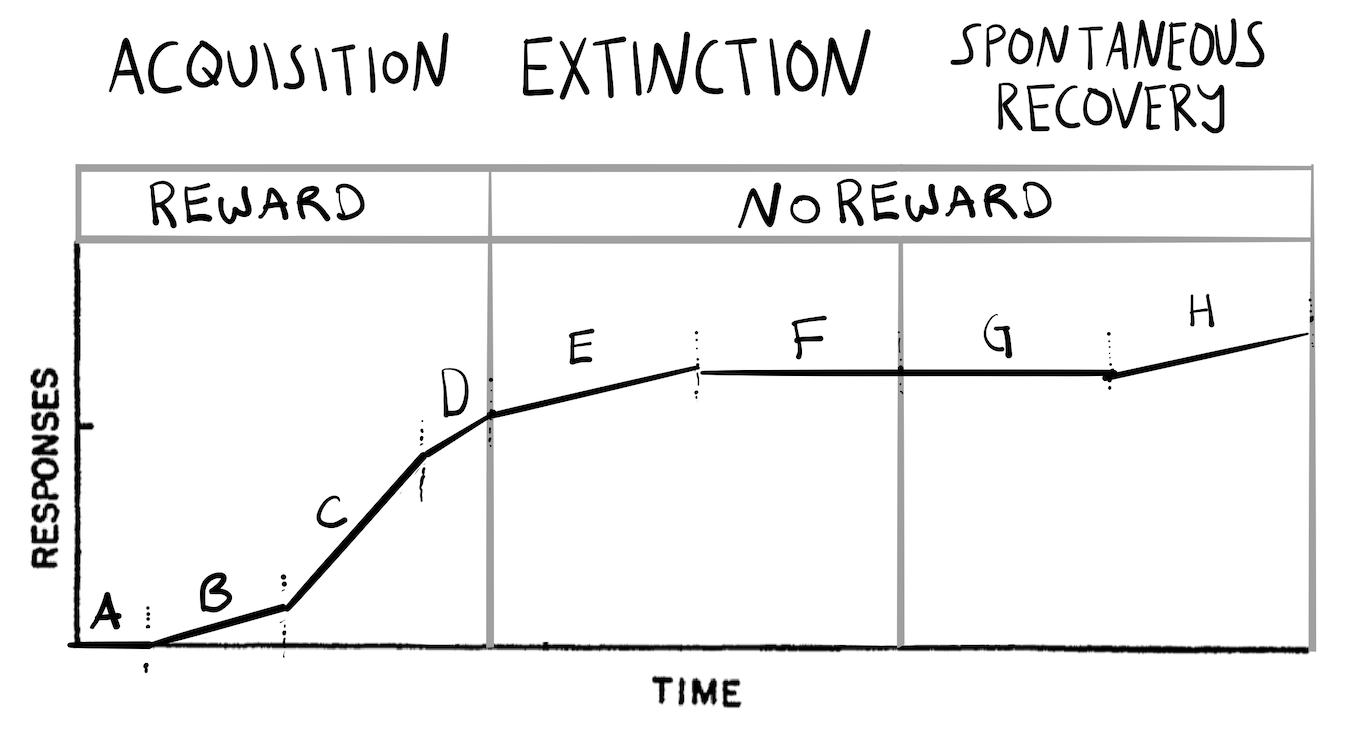
\includegraphics[width=1\linewidth]{imgs/Skinner_description} \end{center}

The rat has an initial \textbf{reflex reserve} giving it some propensity to make the reflex. Prior to acquisition, some unknown impulse causes a \textbf{threshold} to be reached, and the \textbf{reflex} is spontaneously emitted. The impulse doesn't occur often, or the threshold is very high, so the \textbf{reflex strength} is low overall because it occurs infrequently.

During the acquisition phase the animal is inserted into the box. During \emph{A}, the reflex threshold is not exceeded, and no reflexes are emitted. During \emph{B}, some impulse spontaneously passed the reflex threshold, and the reflex was emitted at a low rate. Now, we must invoke another law:

\begin{quote}
``\textbf{The Law of Conditioning of Type R} If the occurrence of an operant is followed by presentation of a reinforcing stimulus the strength is increased.''
\end{quote}

During \emph{B}, the reflex strength increases because it is reinforced. This is observed in behavior as an increase in response rate. During \textbf{C}, the reflex strength, and perhaps even the reflex reserve, has grown substantially. This is shown in behavior by the increase in response rate. However, during \emph{D}, the response rate begins to decline. This could indicate some part of the system is changing, like the threshold is raised requiring a greated impulse to trigger the reflex. Or, the hypothetical \textbf{reflex reserve} could be invoked. The reserve could be ``running dry'', and observed in behavior by a decrease in response rate.

During the extinction phase, reflex continues to occur even though it is not reinforced (E). The continuation of the reflex can be partly described by \textbf{after-discharge}. However, an additional law can be stated to describe the reduction of the rate of responding:

\begin{quote}
\textbf{The Law of Extinction of Type R.} If the occurrence of an operant already strengthened through conditioning is not followed by the reinforcing stimulus, the strength is decreased.
\end{quote}

During E and F, the extinction law describes how the reflex strength is decreased. This is observed in behavior as a rate reduction. Finally, spontaneous recovery (H) can be described by incomplete extinction.

\hypertarget{applications-of-operant-conditioning}{%
\subsection{Applications of operant conditioning}\label{applications-of-operant-conditioning}}

Skinner's operant conditioning research was application oriented from the very beginning. The purpose of exhaustively describing the properties and relations of a simple behavior like lever-pressing was to achieve a generalizable system useful for controlling manipulating other behaviors. Skinner used his methods succesfully for applications like training animals.\footnote{\protect\hyperlink{ref-skinnerHowTeachAnimals1951}{Skinner, B. F. (1951). How to teach animals. \emph{Scientific American}, \emph{185}(6), 26--29. \url{https://doi.org/gmb9rg}}.}

One interesting example is Skinner's \href{https://www.bfskinner.org/project-pigeon/}{project pigeon}, conducted during world war II. Guided missile technology had not been perfected, and missiles were missing their targets. Skinner had the idea to place pigeons inside of missiles, and train them to guide missiles toward their target. Pigeons are very good at pecking, and through operant conditioning, they could be trained to repeatedly peck on a visual target. In this way, a missile could be guided toward a target using the pecking from a pigeon as a steering wheel for the missile. More broadly, operant conditioning techniques are very commonly used in modern animal training.\footnote{\protect\hyperlink{ref-pryorModernAnimalTraining2014}{Pryor, K., \& Ramirez, K. (2014). Modern animal training. \emph{The Wiley Blackwell Handbook of Operant and Classical Conditioning}, 455. \url{https://doi.org/gmb9rj}}.}

Techniques inspired by Skinner's operant conditioning research have also found applications for people. For example, the field of \href{https://en.wikipedia.org/wiki/Applied_behavior_analysis}{applied behavior analysis}. Here, positive and negative reinforcements are used to increase or decrease wanted or unwanted behaviors in humans.

\hypertarget{implications-skinners-utopia}{%
\subsection{Implications: Skinner's Utopia}\label{implications-skinners-utopia}}

Skinner's system of behaviorism was constructed in the tradition of positivism that we have been discussing throughout this chapter. Just like Watson and Tolman, Skinner extended his ideas outside the realm of science to the realm of society. His views on the extension appeared to change over time.

In concluding his book in 1938, Skinner wrote, ``The book represents nothing more than an experimental analysis of a representative sample of behavior. Let him extrapolate who will''. He suggested that anyone who understood what he was saying could easily make the extrapolation themselves, but resisted spelling out any major speculations.

However, just like Watson had envisioned a society guided by his behaviorism, by 1948, Skinner tried his hand at Utopian science fiction and wrote, \href{https://en.wikipedia.org/wiki/Walden_Two}{Walden Two}.\footnote{\protect\hyperlink{ref-skinnerWaldenTwo1948}{Skinner, B. F. (1948). \emph{Walden two}. {Hackett Publishing}}.} The story describes how behavioral engineering through elaborate operant conditioning could improve the lives of 1000 people in a commune, by ensuring they would live happy, productive, and conflict-free lives. The commune also planned to used genetic engineering to eliminate undesirable offspring in the future, and engaged in other eugenic practices like preventing marriage between people with low or incompatible IQs. In a 1976 preface to the book, Skinner reflects on his motivations for writing it, and develops an argument that society will collapse unless it finds ways to modify itself, and that \emph{Walden two} could be a good example of a place to start.

\hypertarget{exit-behaviorism}{%
\section{Exit Behaviorism?}\label{exit-behaviorism}}

This chapter is getting too long, so I will keep this summary short. As I said in the introduction, depending on who is telling the history, behaviorism could be the dark ages of psychology that stood in the way of modern cognitive psychology, or a fore-bearer paving the way. There were many behaviorisms, and many aspects of this collected ``school'' of psychology have been discarded, but many have also be retained.

A commonality in the behaviorism we discussed was that they all followed positivism in rejecting theological and metaphysical ``explanations'' of natural phenomena. For example, they all criticized introspectionist and mentalist psychology as being unscientific, or still in the religious or metaphysical stage. The rejection of mentalism was a denial of cognition, but perhaps only a pragmatic one--that is, it was useful to deny a role for cognition until it was needed in the system, and then it wouldn't be denied anymore. Remember, the goal of the descriptive system was to predict and control behavior. If the system could be constructed without reference to ``cognition'', then ``cognition'' was not necessary for the system to achieve its goal of prediction and control. This was not necessarily a denial that people had cognition.

As we follow the slow transition from behaviorism to cognitivism the wholesale denial of cognitive operations is a position that is often discarded. However, other aspects of positivism are not as readily discarded in cognitivism, such as the format of theorizing, and the rejection of theological and metaphysical considerations. At the same time, cognitivism grows up in a period of post-positive thinking, which leads to a multiplicity of viewpoints. For example, it is possible to have multiple theories for the same phenomena, each with different strengths, limitations, internal working structure (or not), and general usefulness (e.g., for generating new research questions, or applications, or other insights). So, in the years ``post-behaviorism'', we find a diversity of approaches to cognition including some new and a continuance of old approaches.

In the next chapter, we examine the concept of information processing and the introduction of ``information theory'' to psychology. This is a story about how ideas from computer science and communication technology would shape the questions we ask and answer about cognition.

\hypertarget{information-processing}{%
\chapter{Information Processing}\label{information-processing}}

\begin{tabular}{r|l}
\hline
Word Count & Reading Time\\
\hline
11666 & 58.3 minutes\\
\hline
\end{tabular}

\hypertarget{overview-1}{%
\section{Overview}\label{overview-1}}

This chapter overviews \textbf{information processing} as a concept in cognition. I mentioned at the beginning of this textbook, that Ulrich Neisser \footnote{who wrote the first textbook called \emph{Cognitive Psychology} in 1967} defined cognition as ``all processes by which the sensory input is transformed, reduced, elaborated, stored, recovered, and used.''\footnote{\protect\hyperlink{ref-neisserCognitivePsychology1967}{Neisser, 1967}.} Neisser's definition embraces the information processing tradition in cognition. Sensory input contains ``information'' about the world, and cognition is characterized as the ``processing'' of that information. However, just like there were many forms and ideas about behaviorism, there are different forms and ideas about information processing in cognition. We will examine the notions of \emph{processing stages}, \emph{information}, and \emph{capacity limitations}, which became popular research topics around the 1950s and 60s.

Some alliterative themes about cognitive research are also introduced. For example, we begin the chapter with the \emph{four Rs}, referring to the industrial, technological, digital and ``cognitive'' revolutions. The first three revolutions introduced many new machines that changed the course of human history. Some of these machines also had an influence on explanation of cognition. In particular, over the decades, mechanistic explanations of cognitive phenomena have been closely inspired by the working elements of machines modern for the time. In this chapter, we introduce the ``assembly-line'', ``telephone'', and ``computer'' metaphors of cognition, and examine how the first two technologies shaped the concept of information processing. The computer metaphor will be expanded upon in later chapters.

\hypertarget{four-revolutions-industrial-technological-digital-and-cognitive}{%
\section{Four Revolutions: Industrial, Technological, Digital, and ``Cognitive''}\label{four-revolutions-industrial-technological-digital-and-cognitive}}

``Revolution'' is used to describe periods in history where some innovation led to dramatic changes in society. For example, the \href{https://en.wikipedia.org/wiki/Industrial_Revolution}{industrial revolution} in Western Europe and America involved creating large-scale machines, factories and \emph{assembly-lines} to mechanize the means of production; and, is credited with launching the world into an unprecedented period of sustained growth (e.g., population growth, socio-economic growth). The \href{https://en.wikipedia.org/wiki/Second_Industrial_Revolution}{second industrial revolution} (AKA technological revolution), brought the introduction of electricity, \emph{telephones for communication}, planes, trains, and automobiles for transportation, and new systems for infrastructure like sewage and water supply networks. Eras associated with the introduction of technology are also described in terms of ages, like the \href{https://en.wikipedia.org/wiki/Machine_Age}{machine age}, \href{https://en.wikipedia.org/wiki/Atomic_Age}{atomic age}, \href{https://en.wikipedia.org/wiki/Jet_Age}{jet age}, \href{https://en.wikipedia.org/wiki/Space_Age}{space age}. A more recent revolution was the \href{https://en.wikipedia.org/wiki/Digital_Revolution}{digital revolution} involving introduction of \emph{computer technology}, which led into the \href{https://en.wikipedia.org/wiki/Information_Age}{information age}. According to wikipedia, the next age could be the \href{https://en.wikipedia.org/wiki/Imagination_age}{imagination age} involving immersive virtual reality experiences and an economy primarily driven by ``imagination work'' \footnote{hmmm\ldots{}}.

Psychologists have also used ``revolutionary'' terms to describe historical periods of research in psychology. For example, the ``cognitive revolution'' generally refers to the period of experimental psychology following ``radical behaviorism''. The figurative imagery implies that ``cognitive psychologists'' rebelled and overthrew the ``behaviorist orthodoxy''. However, the transition between the two schools of thought was very gradual, and several aspects of behaviorism were retained as a part of modern cognition.\footnote{\protect\hyperlink{ref-greenwoodUnderstandingCognitiveRevolution1999}{Greenwood, J. D. (1999). Understanding the {``cognitive revolution''} in psychology. \emph{Journal of the History of the Behavioral Sciences}, \emph{35}(1), 1--22. \url{https://doi.org/ffh4k7}}; for additional descriptions of the ``cognitive revolution'' see, \protect\hyperlink{ref-millerCognitiveRevolutionHistorical2003}{Miller, George A. (2003). The cognitive revolution: A historical perspective. \emph{Trends in Cognitive Sciences}, \emph{7}(3), 141--144. \url{https://doi.org/b7wqdk}}; \protect\hyperlink{ref-sperryImpactPromiseCognitive1993}{Sperry, R. W. (1993). The impact and promise of the cognitive revolution. \emph{American Psychologist}, \emph{48}(8), 878. \url{https://doi.org/cr7svp}}.} In this sense, ``revolution'' is not a great metaphor for the emergence of cognitive psychology . For example, cognitive psychologist \href{https://en.wikipedia.org/wiki/George_Mandler}{George Mandler} notes, ``The term `revolution' is probably inappropriate---there were no cataclysmic events, the change occurred slowly in different sub-fields over some 10 to 15 years, there was no identifiable flash-point or leader, and there were no Jacobins.''\footnote{\protect\hyperlink{ref-mandlerOriginsCognitiveEvolution23}{Mandler, G. (23 C.E.--2002). Origins of the cognitive (r)evolution. \emph{Journal of the History of the Behavioral Sciences}, \emph{38}(4), 339--353. \url{https://doi.org/d4grcn}}.}

It is no secret that people use metaphors all of the time. And, in later chapter we will discuss a central role for metaphors as a process in cognition. For example, metaphors can shape how people think of one thing in terms of another. The ``cognitive revolution'' could lead you to imagine a fight against the ruling behaviorists. In this case, the revolution metaphor is not very fitting or insightful. The metaphor does not illuminate important historical aspects of the behaviorism-cognitive transition. Using the metaphor could exaggerate the importance of some historical elements over others by highlighting attention toward elements that fit the metaphor, and misdirecting examination of elements that do not fit the metaphor. However, in other cases a metaphorical relationship can fit very well, be useful for explanation, and even generate insights.

As I will describe briefly in the next section, metaphors are very commonly used to describe how cognition works. We will use technological revolutions as metaphors to describe concepts of ``information processing'' in cognition. The introduction of ``information processing'' concepts occurred during the transition from behaviorism to cognitivism, and involved mechanistic metaphors from the industrial revolution (the factory and assembly line), and the technological revolution (the telephone).

\hypertarget{assembly-line-metaphor-of-cognition}{%
\subsection{Assembly-line metaphor of cognition}\label{assembly-line-metaphor-of-cognition}}

\begin{floatright50}
\textbf{A crayon assembly line}

\end{floatright50}

A major innovation of the industrial revolution was the introduction of machines and factories to automate production. These are physical devices that process and transform raw materials into other refined states, that are further transformed and or assembled into goods or final products. For example, a factory assembly-line for making crayons involves successive processing stages, such as: heating wax in vat, coloring and stirring the liquid, filtering, pouring and drying and forming the wax into malleable rolls, extruding the rolls of colored wax through perforated metal plates (with holes the size of crayons), drying the newly formed crayons, and placing them in machines to wrap and package them. The assembly-line metaphor is also used in cognition, and refers to the idea that there are separate stages of processing that transform the ``raw materials'' of sensation into the ``final products'' of cognition and action. We examine this metaphor in the section on Donders and his use of mental chronometry to measure assumed stages of processing.

\hypertarget{telephone-metaphor-of-cognition}{%
\subsection{Telephone metaphor of cognition}\label{telephone-metaphor-of-cognition}}

A major innovation of the technological revolution was the introduction of \href{https://en.wikipedia.org/wiki/Telecommunication}{communication technology} like the \href{https://en.wikipedia.org/wiki/Electrical_telegraph}{telegraph} and \href{https://en.wikipedia.org/wiki/Telephone}{telephone}. This technology allowed people to communicate in real-time over long distances, from one device connected by wire to another device. There was a great demand for telephone technology, and the demand was met by creating a massive network of wires to connect phones to each other. Before automation, the telephone network was managed by human operators who worked at central nodes in the network. A caller who picked up a phone to place a call would be immediately connected to a human telephone operator, and would ask to be connected to another phone. The operator received the instructions and the made the physical connection in the network to connect the incoming call to the destination phone. Around the time of world war II, several psychologists began using elements of the telephone system as a metaphor for cognitive processing. After Donders' processing stages, we examine the concept of ``information'' processing which was borrowed largely from telecommunication theory and technology.

\hypertarget{computer-metaphor-of-cognition}{%
\subsection{Computer metaphor of cognition}\label{computer-metaphor-of-cognition}}

A major innovation of the digital revolution was the introduction of computing technology. The rise of the computer sciences also occurred in tandem with the growth of modern cognitive psychology. For example, the ``\href{https://en.wikipedia.org/wiki/Cognitive_science}{cognitive sciences}'' are considered an interdisciplinary discipline with major contributions from and cross-fertilization of ideas between cognitive psychology, computer science, philosophy, linguistics, neuroscience and anthropology. Like other transformational technology, computers have been used as prominent metaphors for cognition. Sometimes cognitive theories are very literal with the metaphor, and cognition is broken down into parts resembling actual physical components of a digital computer. In other cases, cognition is described in terms of more abstract computational processes and algorithms rather than concrete components. Although computers are highly relevant to the ``information processing'' theme of this chapter, further elaboration on the computational metaphor of cognition will be reserved for upcoming chapters.

\hypertarget{the-mechanization-of-cognition}{%
\section{The mechanization of cognition}\label{the-mechanization-of-cognition}}

Our first metaphorical theme is between cognition and machines in the industrial revolution. We have already seen examples of the metaphor. For example, Descartes likened human and animal physiology to a complicated plumbing machine, like the one he saw in the royal gardens. However, Descartes was a dualist who argued that the biological machine of the human body was merely a receptacle for psychic forces. Nevertheless, he inspired physiological psychology and modern neuroscience, which have the aims of explaining cognitive processes in terms of their physical/bio-chemical substrates.

Machines offer a reductive perspective on explanation, where the goal is to explain how the parts of a machine work together to produce the behavior of the machine. Man-made machines are physical contraptions whose actions obey the known physical laws of the universe, and whose various states are determined by how the machine is assembled and connected together. Presumably, the person(s) who put a machine together in some sense understood the machine well enough to put it together and make it work. At the same time, I don't know every detail of how much of the technology I use in daily life works. However, I assume that someone can explain how my phone works. Similarly, if humans encountered an alien technology, and no human knew how it worked, then I would guess that many people would attempt to ``\href{https://en.wikipedia.org/wiki/Reverse_engineering}{reverse-engineer}'' the machine to figure out how it works. Reverse-engineering involves de-constructing an existing machine into its constituent parts to figure out how the machine works. For that matter, humans and animals are space creatures living on the planet earth, and research in psychology and neuroscience is attempting to ``reverse-engineer'' how our biological machines work.

Machines set a compelling standard for explanation, especially if the standard is to demonstrate explanation by successfully manufacturing a working machine. For example, if the inner workings of the machine of cognition can be ``explained'' to this standard, then along with other technology, cognition could be manufactured and innovated upon. By analogy, this could include ways to repair, restore, and preserve cognition, as well as create new ways for cognition to work and function. As with the prospects of behavioral engineering, cognitive technologies also raise a host of ethical questions.

At the same time, psychology does not always have the goal of achieving a machine-based explanation. For example, some of the behaviorists in the previous chapter deliberately side-stepped mechanistic explanations as a goal. For example, Skinner acknowledged that behavior was ultimately rooted in physical mechanisms, but he argued that behavior itself could also be studied at a macroscopic level, without referring to it's microscopic mechanisms. He sometimes used terms that loosely referred to mechanisms. For example, a ``reflexes'' had ``strength'', and were emitted after some ``impulse'' reached a ``threshold''. All of these terms could refer to various physical mechanisms; however, Skinner was careful to say that none of them were intended to refer to any real mechanism. They were simply abstract and arbitrary terms in his system that he could have chosen different names for. As a result, many components of Skinner's theory were not intended to be explained at a lower-level.

For example, you might ask, how does an impulse surpass a threshold and trigger a reflex, what is the mechanism? In Skinner's system this question could be viewed as incoherent by definition. He defined those terms not to have any reference to physical mechanisms. Of course, it is possible to wonder about what physiological mechanisms do give rise to the behaviors in Skinner's descriptive system, but the investigation of such mechanisms was not in the same domain as behaviorism.

In my view, behaviorists had an awkward relationship with mechanistic explanations. They were critical of domains that lacked mechanisms, such as mentalistic and introspectionist psychology; but, also carefully avoided having to describe mechanisms for their domain of psychology. Instead, they were content with terms that had metaphorical connotations of mechanisms, as long as the terms were operationally defined and useful for a descriptive system of behavior.

As we step past the behaviorist era in to the cognitive one, we will see a shift in explanatory style from purely descriptive systems to a greater emphasis on mechanistic lines of questioning and mechanistic accounts of cognitive processes. This shift sometimes involves actual physical mechanisms in the brain, body, and environments; but, the shift also involves usage of metaphorical mechanisms. Metaphorical mechanisms may sound like an oxymoron, but they are very common in science. The general strategy is first to find a simple model system that is ``like'' a more complicated system under investigation; and then use the simple model as a ``metaphor'' to describe or generate insights about the more complicated system. In the next section we look at the concept of mental processing stages and the assembly-line metaphor from the industrial revolution.

\hypertarget{donders-processing-stages}{%
\section{Donders' Processing Stages}\label{donders-processing-stages}}

Up to this chapter we have traced a line through psychology from Galton in 1865 to the period of behaviorism. There are several other starting points we could have chosen. For example, in the same year, 1865, Dutch Physiologist F. C. Donders presented behavioral experiments on human reaction times to support the beginnings of a mechanistic theory of cognitive operations.\footnote{\protect\hyperlink{ref-kosterPreface1969}{Koster, W. G. (1969). Preface. In W. G. Koster (Ed.), \emph{Attention and {Performance II}: Proceedings of the donders centenary symposium on reaction time}. {North-Holland Publishing Company}}.} I will characterize Donders work as using an assembly line metaphor of cognition. In an assembly line, raw material is sent from one stage of processing to another, and a product is formed at the end of the whole process. In cognition, sensory input is the raw material that is transformed in successive stages of processing. In an assembly-line, each stage of processing does a particular job, and takes an amount of time. Similarly, in cognition, Donders assumed that there were individual stages of processing (for different jobs of cognition), and that each job took some amount of time. He developed a method for identifying different stages of cognitive processing and estimating how long each of them took to complete. His was work was translated into English with the title, ``On the speed of mental processes.''\footnote{\protect\hyperlink{ref-dondersSpeedMentalProcesses1868}{Donders, F. C. (1868--1969). On the speed of mental processes. In W. G. Koster (Ed.), \emph{Attention and {Performance II}}. {North-Holland Publishing Company}}.}

\hypertarget{donders-mental-chronometry-and-processing-stages}{%
\subsection{Donders mental chronometry and processing stages}\label{donders-mental-chronometry-and-processing-stages}}

Donders was a physiologist and impressed with emerging work on the speed of nerve conduction. Earlier physiologists (Johannes Muller) said the velocity of nerve conduction could be infinitely fast, or unknowable. But, in 1849, \href{https://en.wikipedia.org/wiki/Hermann_von_Helmholtz}{Hermann von Helmholtz}, succeeded in measuring nerve transmission speeds in a frog in the range of 24-36 meters per second.

The empirical observation that nerve conduction was not infinitely fast was very important for Donders. As a physiologist he assumed that thinking processes of the mind were controlled by organs in the brain. If the exchange of signals in the nervous occurred infinitely fast, he assumed that processes of thought might also occur infinitely fast. However, the discovery that nerves had physical properties limiting how fast they conducted signals suggested to Donders thoughts might have some measurable speed, so he set out record the speed thought.

\hypertarget{physiological-reaction-time}{%
\subsection{Physiological reaction time}\label{physiological-reaction-time}}

First, Donders pointed to the concept of physiological reaction time, which came first from astronomy.\footnote{\protect\hyperlink{ref-canalesExitFrogEnter2001}{Canales, J. (2001). Exit the frog, enter the human: Physiology and experimental psychology in nineteenth-century astronomy. \emph{The British Journal for the History of Science}, \emph{34}(2), 173--197. \url{https://doi.org/cs2z26}}.} Astronomers made observations about locations of heavenly bodies in the sky, and entered positional coordinates and times of observations about those bodies into their record books. Different observatories around the world would share records. Theories of planetary motion could be tested by comparing the predictions about where planets should be at different times to the recorded data about where planets were observed to be at different times. There were discrepancies between theory and data. Astronomer Adolphe Hirsch wondered how much of the discrepancies were due to human error. Some of the human observers might have slightly faster perceptions than other human observers, and this could introduce error into the entries they made into the astronomical records. Hirsch set out to measure each observers ``physiological'' reaction time.

Imagine you were an astronomer about to look at a star through a telescope. As soon as the light from the star hits your eyeball, how long will it take for you to react to the light? Donders called this ``physiological time'' in reference to the time it would take for the light stimulus to be transduced through the eye into nervous activity that would eventually lead to a muscle response. Hirsch had already developed methods to precisely measure an individual's ``physiological reaction time'', and used those measures to correct the astronomical records from human error. Donders had a different usage for the method. He wrote:

\begin{quote}
``The idea occurred to me to interpose into the process of the physiological time some new components of mental action. If I investigated how much this would lengthen the physiological time, this would, I judged reveal the time required for the interposed term.''
\end{quote}

\hypertarget{donders-mental-reaction-times}{%
\subsection{Donders mental reaction times}\label{donders-mental-reaction-times}}

Donders conducted many human reaction time experiments using tactile, visual and auditory stimuli. All of the experiments used a similar method. A subject was presented with a stimulus, and they responded to the stimulus as quickly and accurately as possible. Donders measured reaction times, which was defined as the amount of time between the onset of the stimulus and a subsequent response. Note, reaction times continue to be used in cognitive psychology, and their definition remains the same.

A basic question was whether different sense organs had different physiological reaction times. But, Donders was more interested in the additional ``mental'' time it might take to perform increasingly complex tasks before making a response to the stimuli. The tasks that Donders used to increase complexity are still widely used. In the remaining description of Donders work, I will use the modern terms for the tasks, and present a generic summary of Donders findings and conclusions.

\begin{floatright25}
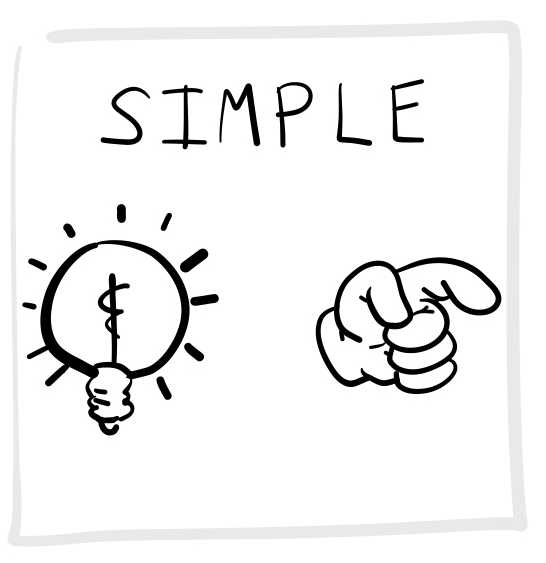
\includegraphics[width=1\linewidth]{imgs/Donders_simple}

\end{floatright25}

The most basic reaction time task is called a \emph{simple reaction time task}. In this task, subjects are presented with a stimulus, and asked to respond to as quickly as possible, as soon as they detect it. Donders would consider the reaction times from this task as ``physiological reaction times''.

\begin{floatright25}
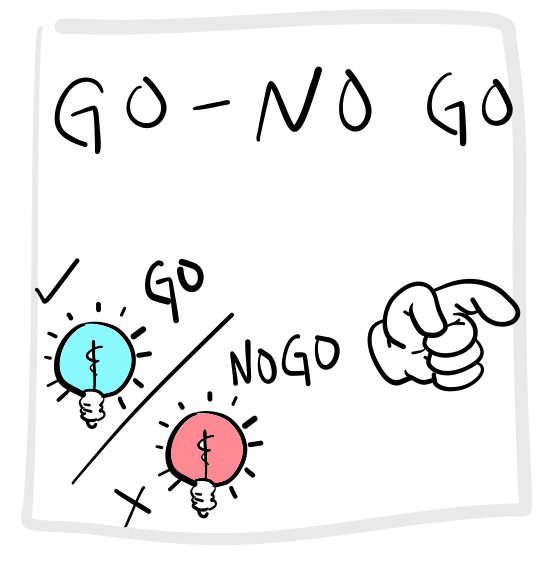
\includegraphics[width=1\linewidth]{imgs/Donders_GoNoGo}

\end{floatright25}

Donders invented the idea of having subjects perform a slightly more complicated task that is now referred to as the \emph{GO-NO GO} task. In this task, subjects are presented with a stimulus, but they only make a response if the stimulus is the target stimulus. For example, one might see a blue or red stimulus, and the response would be required only if the stimulus was blue (a GO response). No response would be required if the stimulus was red (a NO GO trial).

\begin{floatright25}
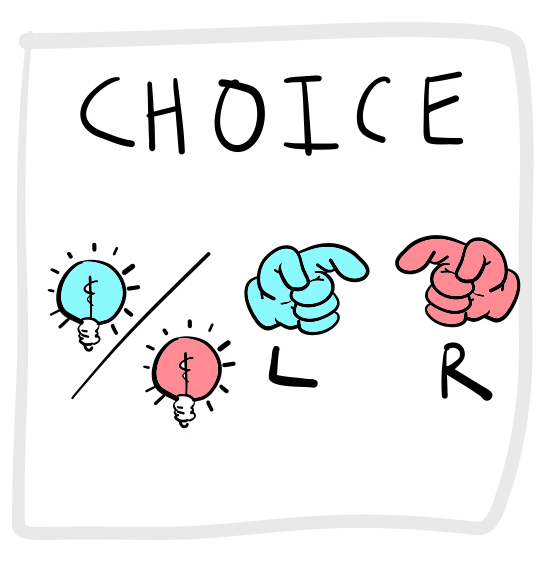
\includegraphics[width=1\linewidth]{imgs/Donders_Choice}

\end{floatright25}

An even more complicated version of the task is referred to as an \emph{alternative forced-choice task}. For example, a subject could be asked to respond to a blue stimulus by pressing a left button, and to respond to a red stimulus by pressing a right button. This would be called a 2-AFC (two-alternative forced choice) task, or a choice reaction time task.

\hypertarget{donders-subtractive-stage-logic}{%
\subsection{Donders subtractive stage logic}\label{donders-subtractive-stage-logic}}

Donders used subtraction of reaction times between tasks to estimate the speed of mental operations. He assumed that mental operations occurred in successive stages like an assembly line, and that each stage took an average amount time.

\begin{center}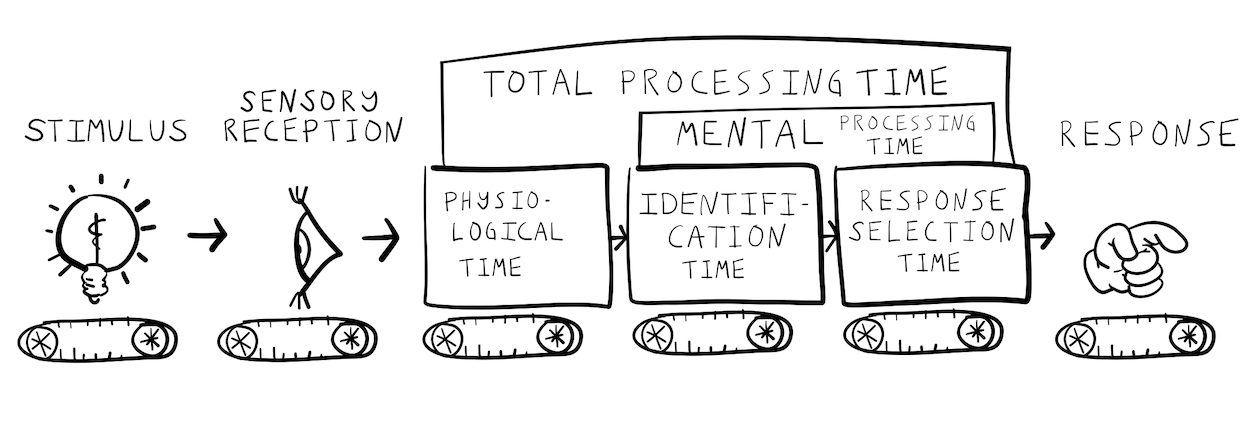
\includegraphics[width=1\linewidth]{imgs/Donders_Assembly} \end{center}

The fastest reaction time should be the physiological time given by the simple reaction time task. This one involved a minimum of mental processing. Reaction times should increase in length if mental processing had to occur before a response was made.

\begin{center}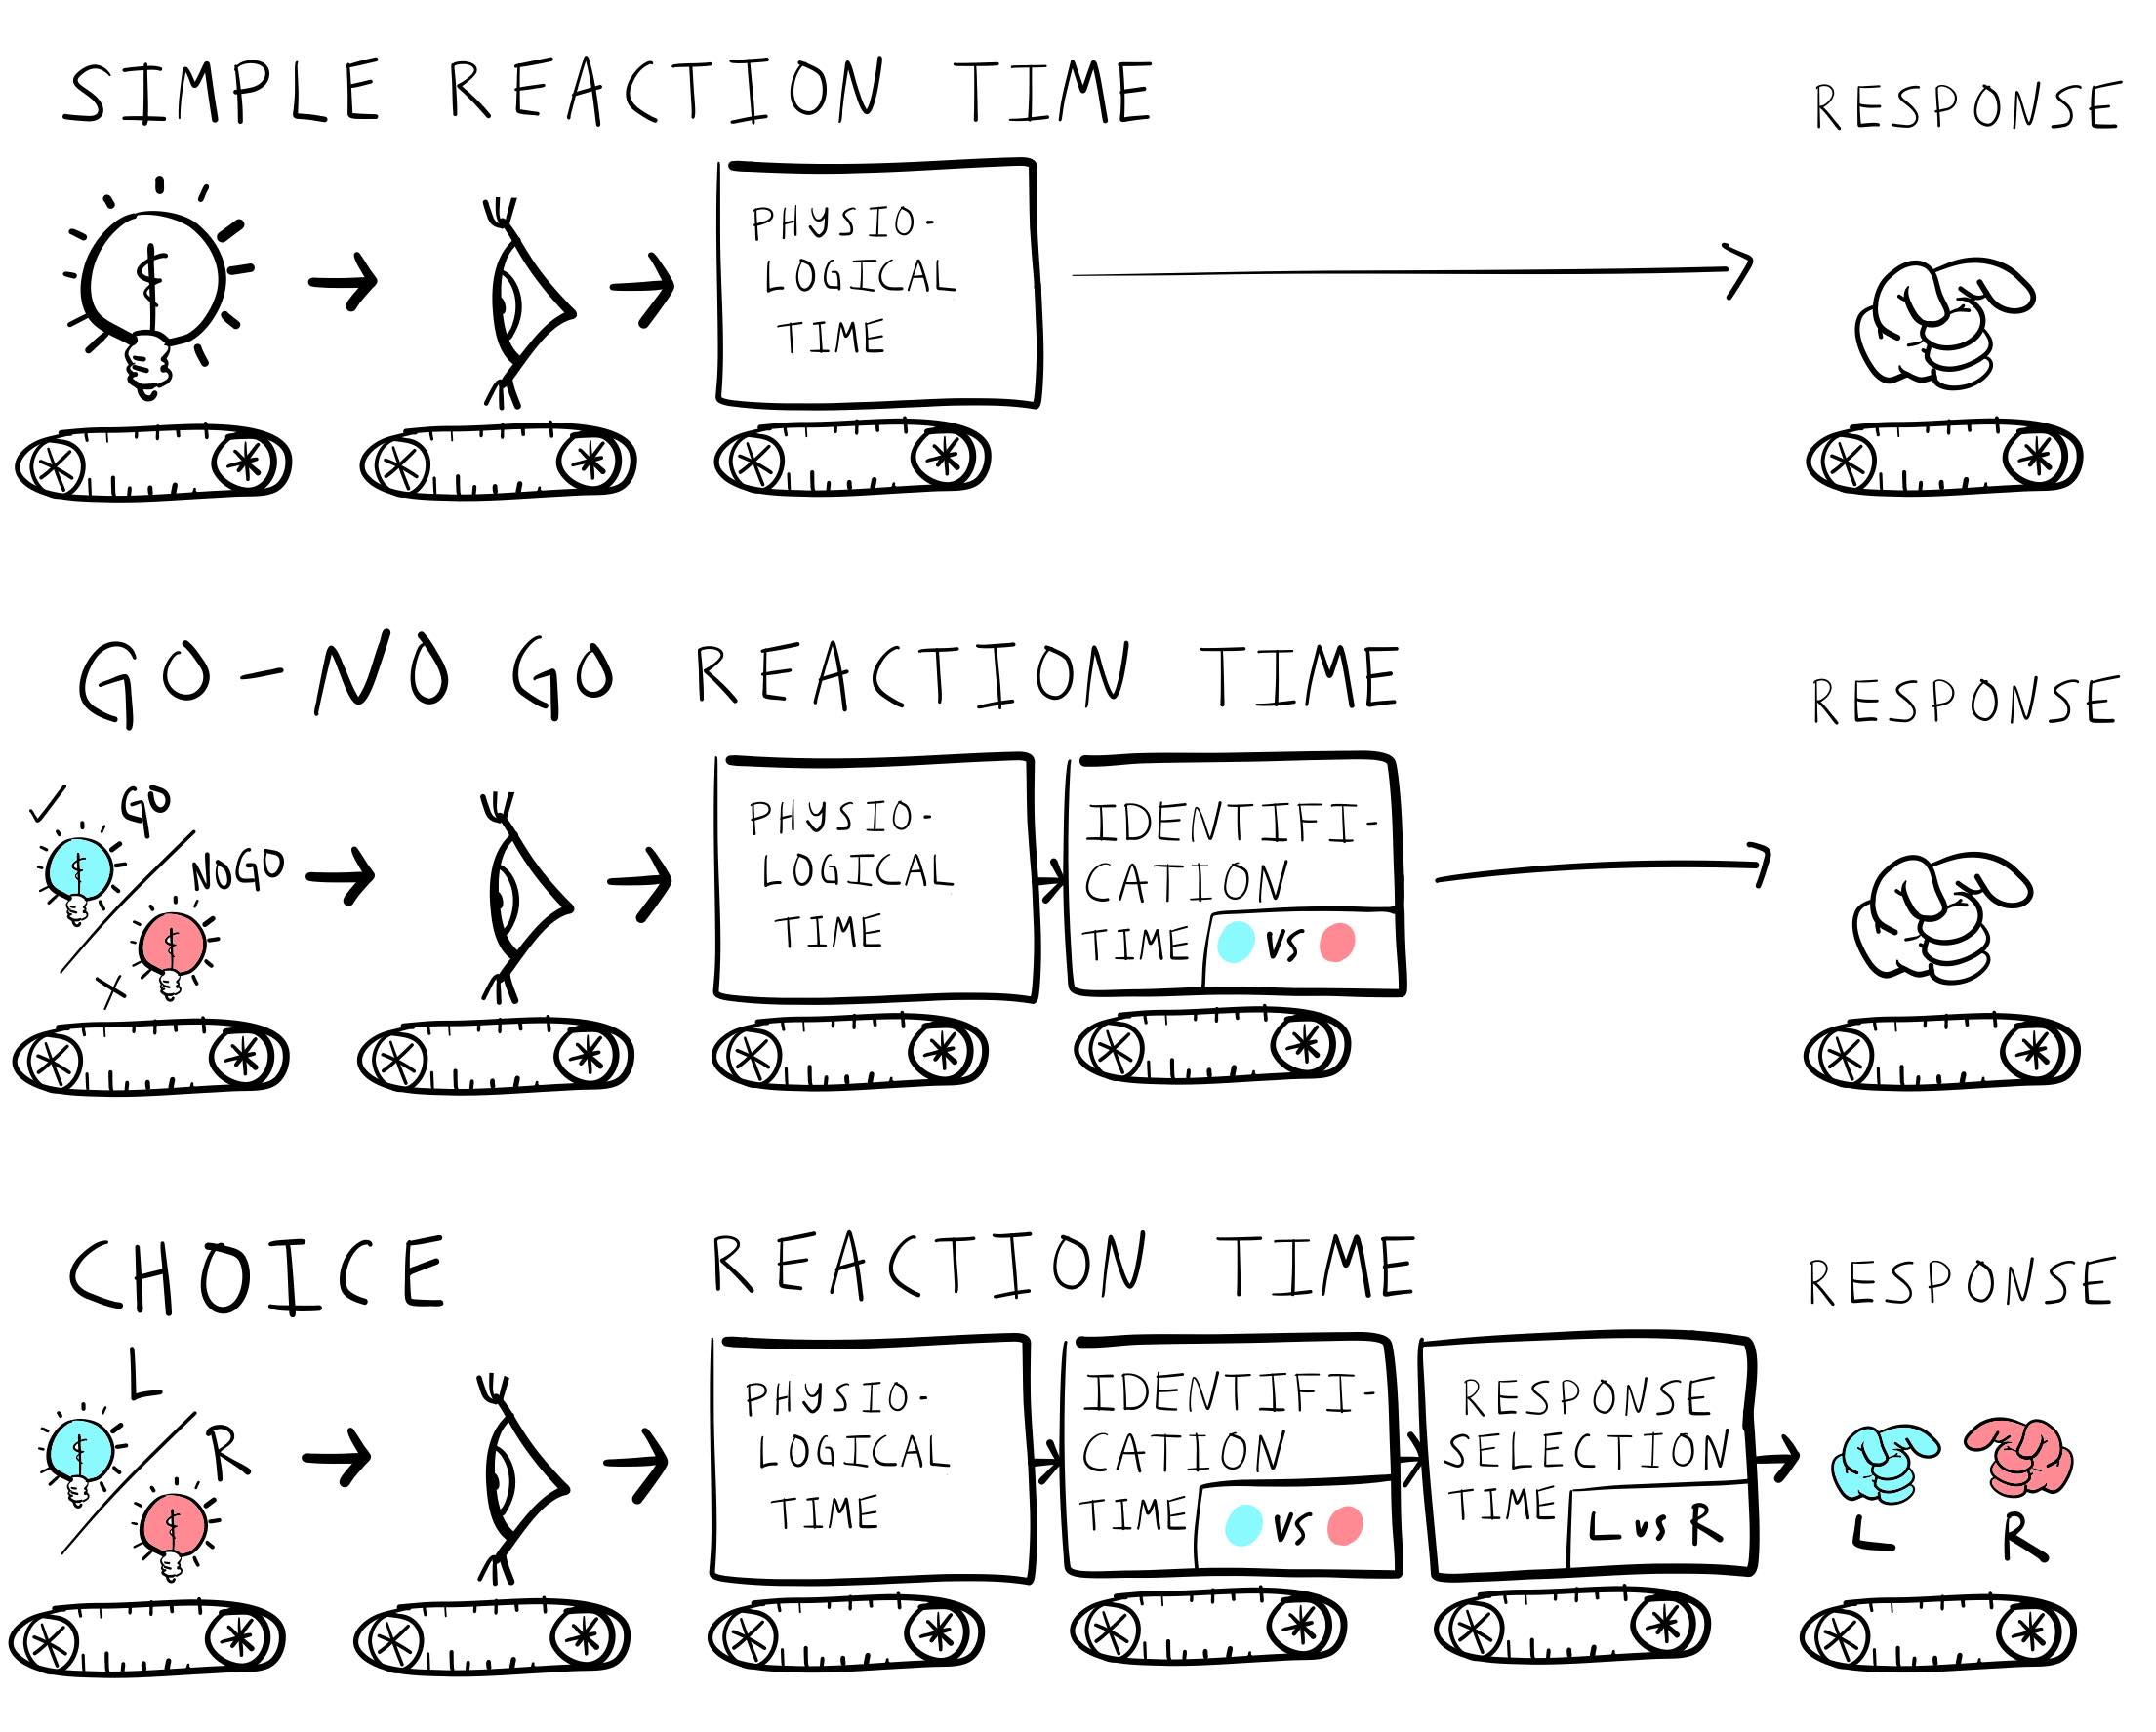
\includegraphics[width=1\linewidth]{imgs/Donders_task_stages} \end{center}

For example, the GO-NO GO task should produce a longer reaction time than the simple reaction time task. This is because the task requires an additional mental operation of stimulus identification. In the GO-NO GO task, the stimulus must be identified as the target stimulus before a response is made.

\begin{center}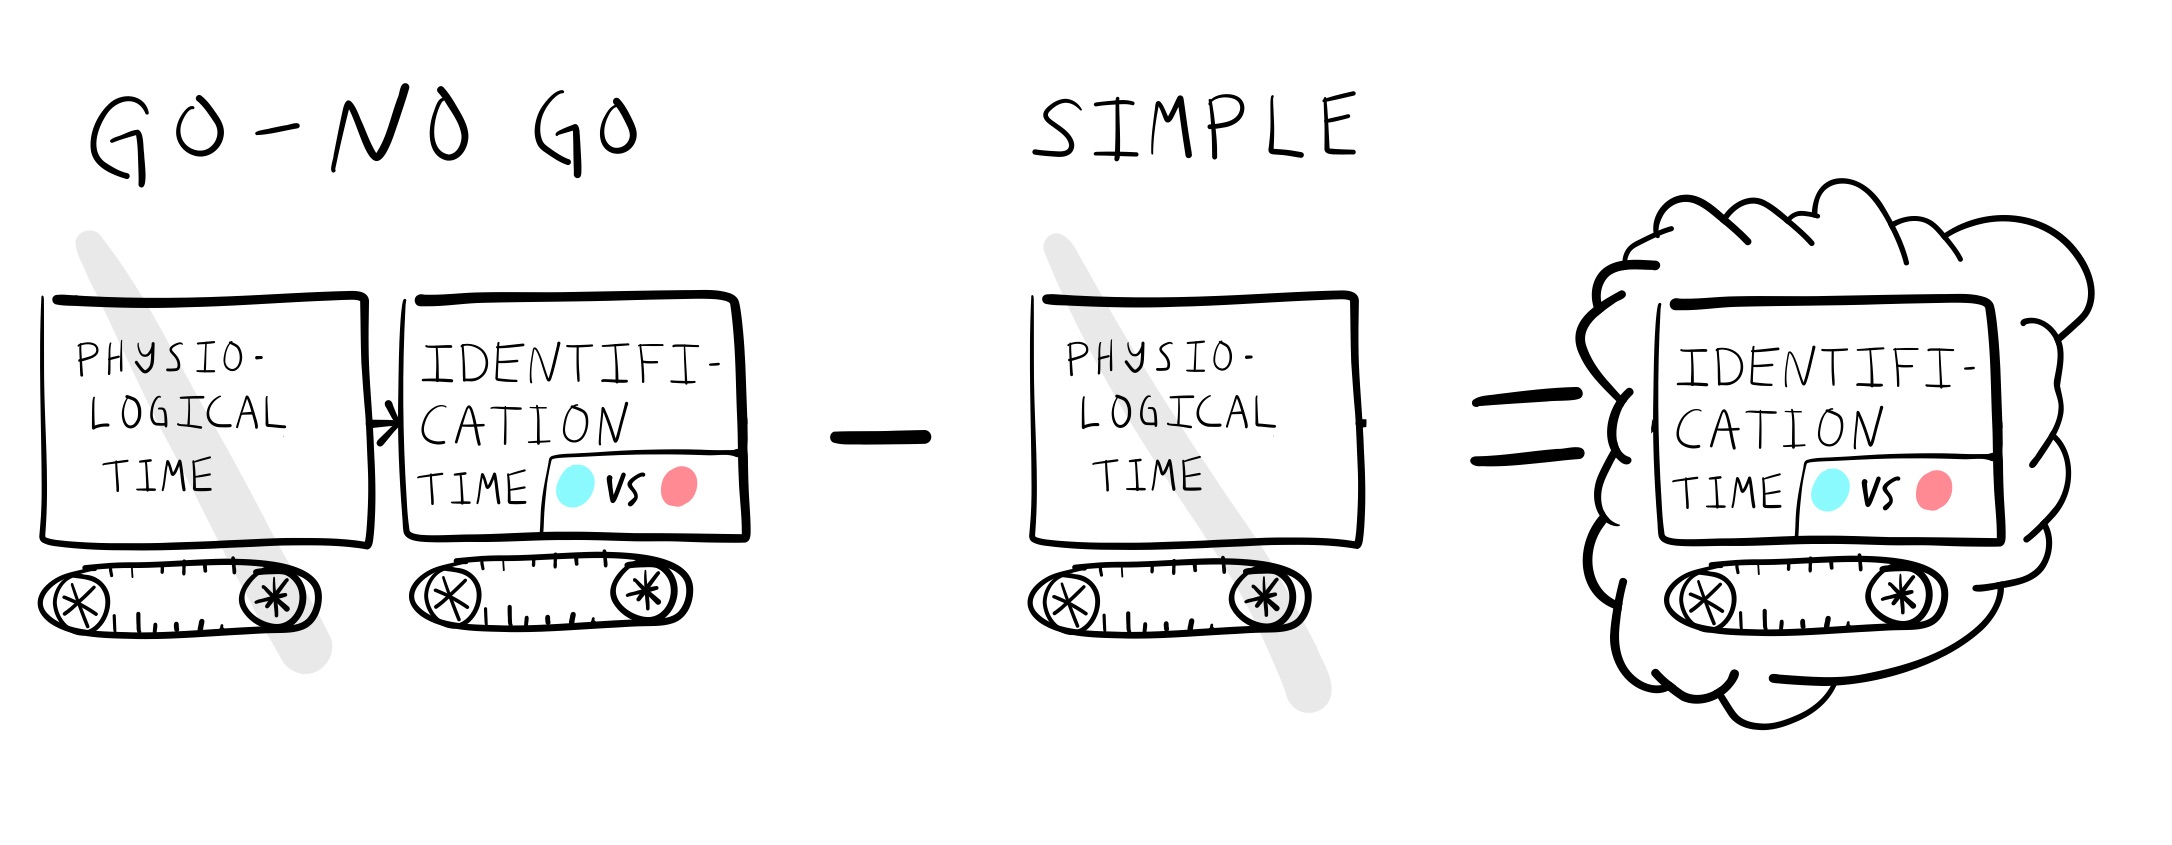
\includegraphics[width=1\linewidth]{imgs/Donders_id_time} \end{center}

If it took 170 milliseconds to make a response in the GO - NO GO task, and 150 milliseconds to make a response in the simple reaction time task, Donders took the difference of 20 milliseconds (by subtraction 170-150 = 20) to indicate the time taken by the mental operation. In this example, Donders might say the mental process of identification takes 20 milliseconds.

The subtraction logic could be applied to infer the times associated with subsequent stages of processing. For example, reaction times in a two alternative forced choice task (2AFC) are longer than in a GO-NO GO task. Following Donders logic, a 2AFC task involves yet another mental operation, \emph{response selection}. For example, in this task the stimulus must be identified before a response is made, and then the correct response (e.g., right or left) must be selected before the final response is made. The stage of stimulus identification is assumed to occur before the subsequent stage of response selection.

\begin{center}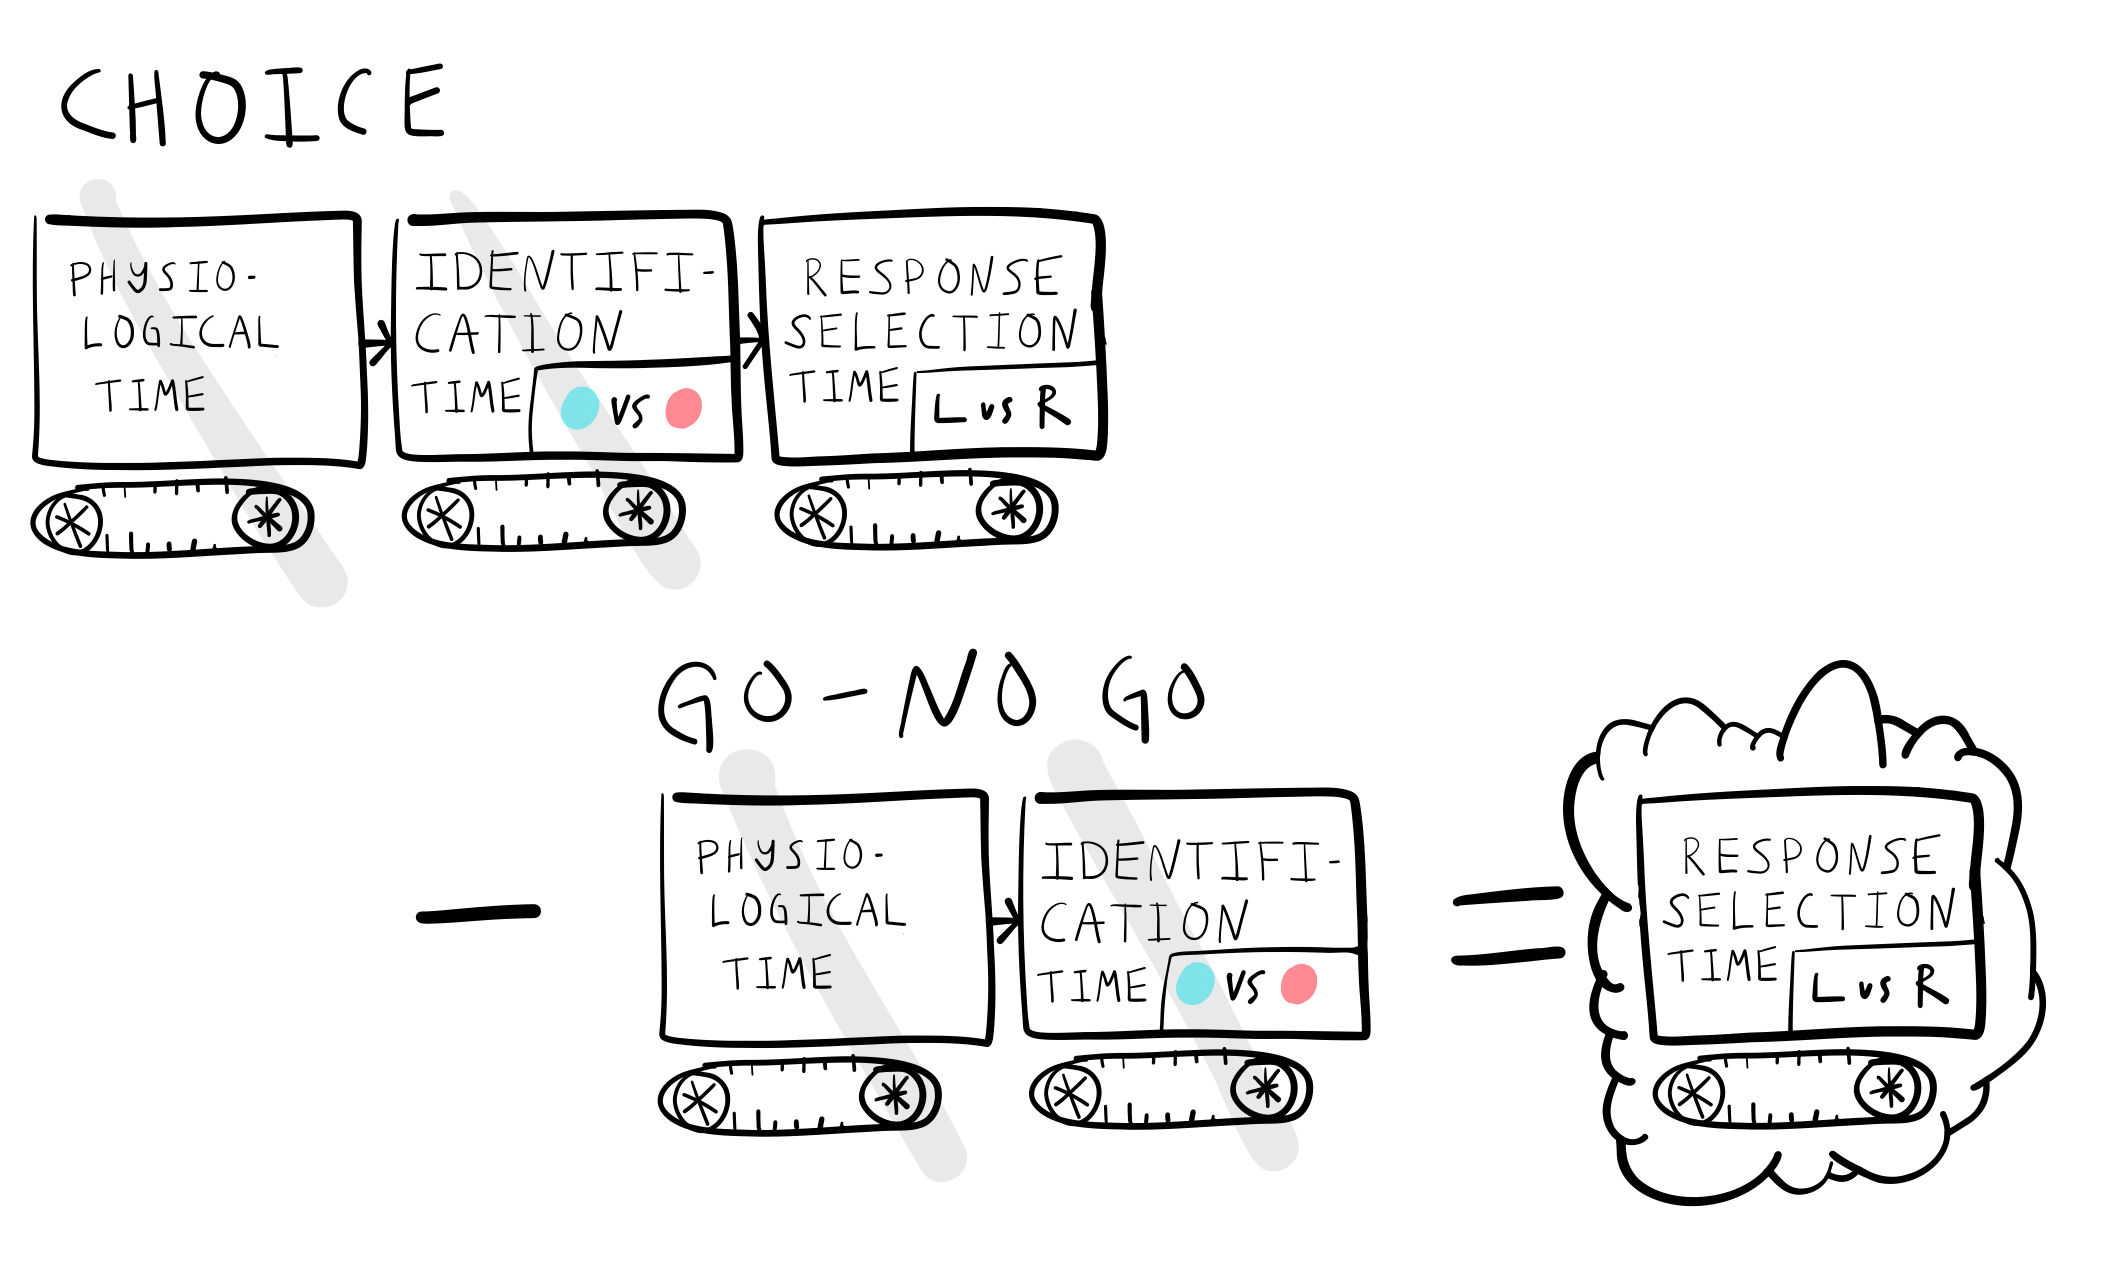
\includegraphics[width=1\linewidth]{imgs/Donders_RT_time} \end{center}

But, by subtracting the reaction time in the 2AFC task, from the reaction time in the GO-NO GO task, Donders argued that the amount of time for response selection could be separated from the amount of time for stimulus identification.

\hypertarget{beyond-donders}{%
\section{Beyond Donders}\label{beyond-donders}}

It has been \(2021 - 1865 = 156\) years since Donders proposed subtraction logic to measure stages of mental processing time. What happened to his subtraction logic, research on human reaction times, and the concept of processing stages?

\hypertarget{subtractive-logic}{%
\subsection{Subtractive logic}\label{subtractive-logic}}

Donders subtractive logic is a nifty idea, but it doesn't necessarily produce correct inferences about cognitive operations. One issue is the distinction between \emph{serial and parallel} processing. If the intervening mental operations between a stimulus and response really do work like a simple \emph{serial} assembly-line, then the subtractive logic can work quite well. In this case, the mental operations occur one after another in series. In this case the total reaction time associated with a task involving two or more mental operations (that occur in serial stages), can be inferred by subtracting reaction times from tasks involving one fewer mental operation. However, the serial assembly line is just a metaphor. A major problem occurs for subtractive logic when operations can be completed in parallel (e.g., at the same time). In this case, different stages of processing might be occurring at the same time, and measurements of additional time spent on a mental task would not necessarily reflect separate stages of processing. Another problem occurs if the stages are unpredictable, and therefore it does not make sense to subtract times that are not constants.

To address some of the inferential problems with subtractive for making inferences about putative processing stages, Saul Sternberg introduced another method called \emph{additive-factors logic}.\footnote{\protect\hyperlink{ref-sternbergDiscoveryProcessingStages1969a}{Sternberg, S. (1969). The discovery of processing stages: {Extensions} of {Donders}' method. \emph{Acta Psychologica}, \emph{30}, 276--315. \url{https://doi.org/ftg756}}.} Finally, subtractive logic became commonly used in neuro-imaging research to find areas of brain activity uniquely correlated with specific task demands.\footnote{\protect\hyperlink{ref-alexanderDondersDeadCortical2015}{Alexander, D. M., Trengove, C., \& van Leeuwen, C. (2015). Donders is dead: Cortical traveling waves and the limits of mental chronometry in cognitive neuroscience. \emph{Cognitive Processing}, \emph{16}(4), 365--375. \url{https://doi.org/f7zgts}}.}

\hypertarget{reaction-time-research}{%
\subsection{Reaction time research}\label{reaction-time-research}}

The measurement of reaction times to make inferences about cognitive processes became widespread, and remains a very common measurement tool in cognition. For example, we already discussed Cattell's associative reaction time research from 1886, which was clearly inspired by Donders. In 1890, Jastrow reviewed the promising uses of reaction time methods in psychology in a book called, \emph{Time relations of mental phenomena}.\footnote{\protect\hyperlink{ref-jastrowTimerelationsMentalPhenomena1890}{Jastrow, J. (1890). \emph{The time-relations of mental phenomena}. {NDC Hodges}}.} Reaction times would be used throughout every decade to study cognitive processes in humans, even throughout the behaviorist period. We will continue to discuss reaction time research throughout this chapter and others.

\hypertarget{processing-stages}{%
\subsection{Processing Stages}\label{processing-stages}}

Donders' concept of mental processing stages disappeared for a while during the behaviorist era. Although some behaviorists (like Tolman and Hull) were willing to speculate about intervening processes between a stimulus and response, other forms of behaviorism were not interested in whatever mental operations might be taking place. As a result, the possibility that there was a mental processing stage for stimulus-identification, response-selection, or other mental operations, was not of scientific interest.

The concept of processing stages came back in different ways, and we will see more examples in the chapters on memory, attention, and computational modeling. As a historical side-note, Donders' ideas become popular again in cognition roughly 100 years after his publication. His centenary was celebrated at the second \href{http://www.attentionandperformance.org}{Attention and Performance} conference in 1968, held in the Netherlands. This invited-speaker conference series still runs today, and publishes books containing the papers presented at the conference. Many of the articles from the early conference years established a role for the concept of processing stages in cognition. One example to mention briefly is the \href{https://en.wikipedia.org/wiki/Psychological_refractory_period}{psychological refractory period}.

\hypertarget{prp-psychological-refractory-period}{%
\subsubsection{PRP: Psychological Refractory Period}\label{prp-psychological-refractory-period}}

British psychologist A. T. Welford drew attention to the \emph{Psychological Refractory Period} in a 1952 paper Welford, A. T.\footnote{\protect\hyperlink{ref-welfordEvidenceSinglechannelDecision1959}{(1959). Evidence of a single-channel decision mechanism limiting performance in a serial reaction task. \emph{Quarterly Journal of Experimental Psychology}, \emph{11}(4), 193--210. \url{https://doi.org/dx8xfc}}.} In the preceding war years a great deal of basic research on human reaction times was conducted for the war effort. For example, the ability to make a quick reaction could be important for a pilot. As a result, empirical studies were conducted to identify useful information about human reaction times. Useful information could include how to make reactions more efficient, or to discover limitations in reaction times that could be addressed. For example, if people are pressing buttons or flicking switches in a cockpit, how should the cockpit be designed to improve the speed and accuracy of the responses?

Welford observed the psychological refractory period from existing reaction time research, and discussed possible explanations of the finding in terms of processing stages. The basic PRP effect was that responding to one stimulus can sometimes delay a response to second stimulus, especially if they are presented quickly, one after the other.

\begin{floatright50}
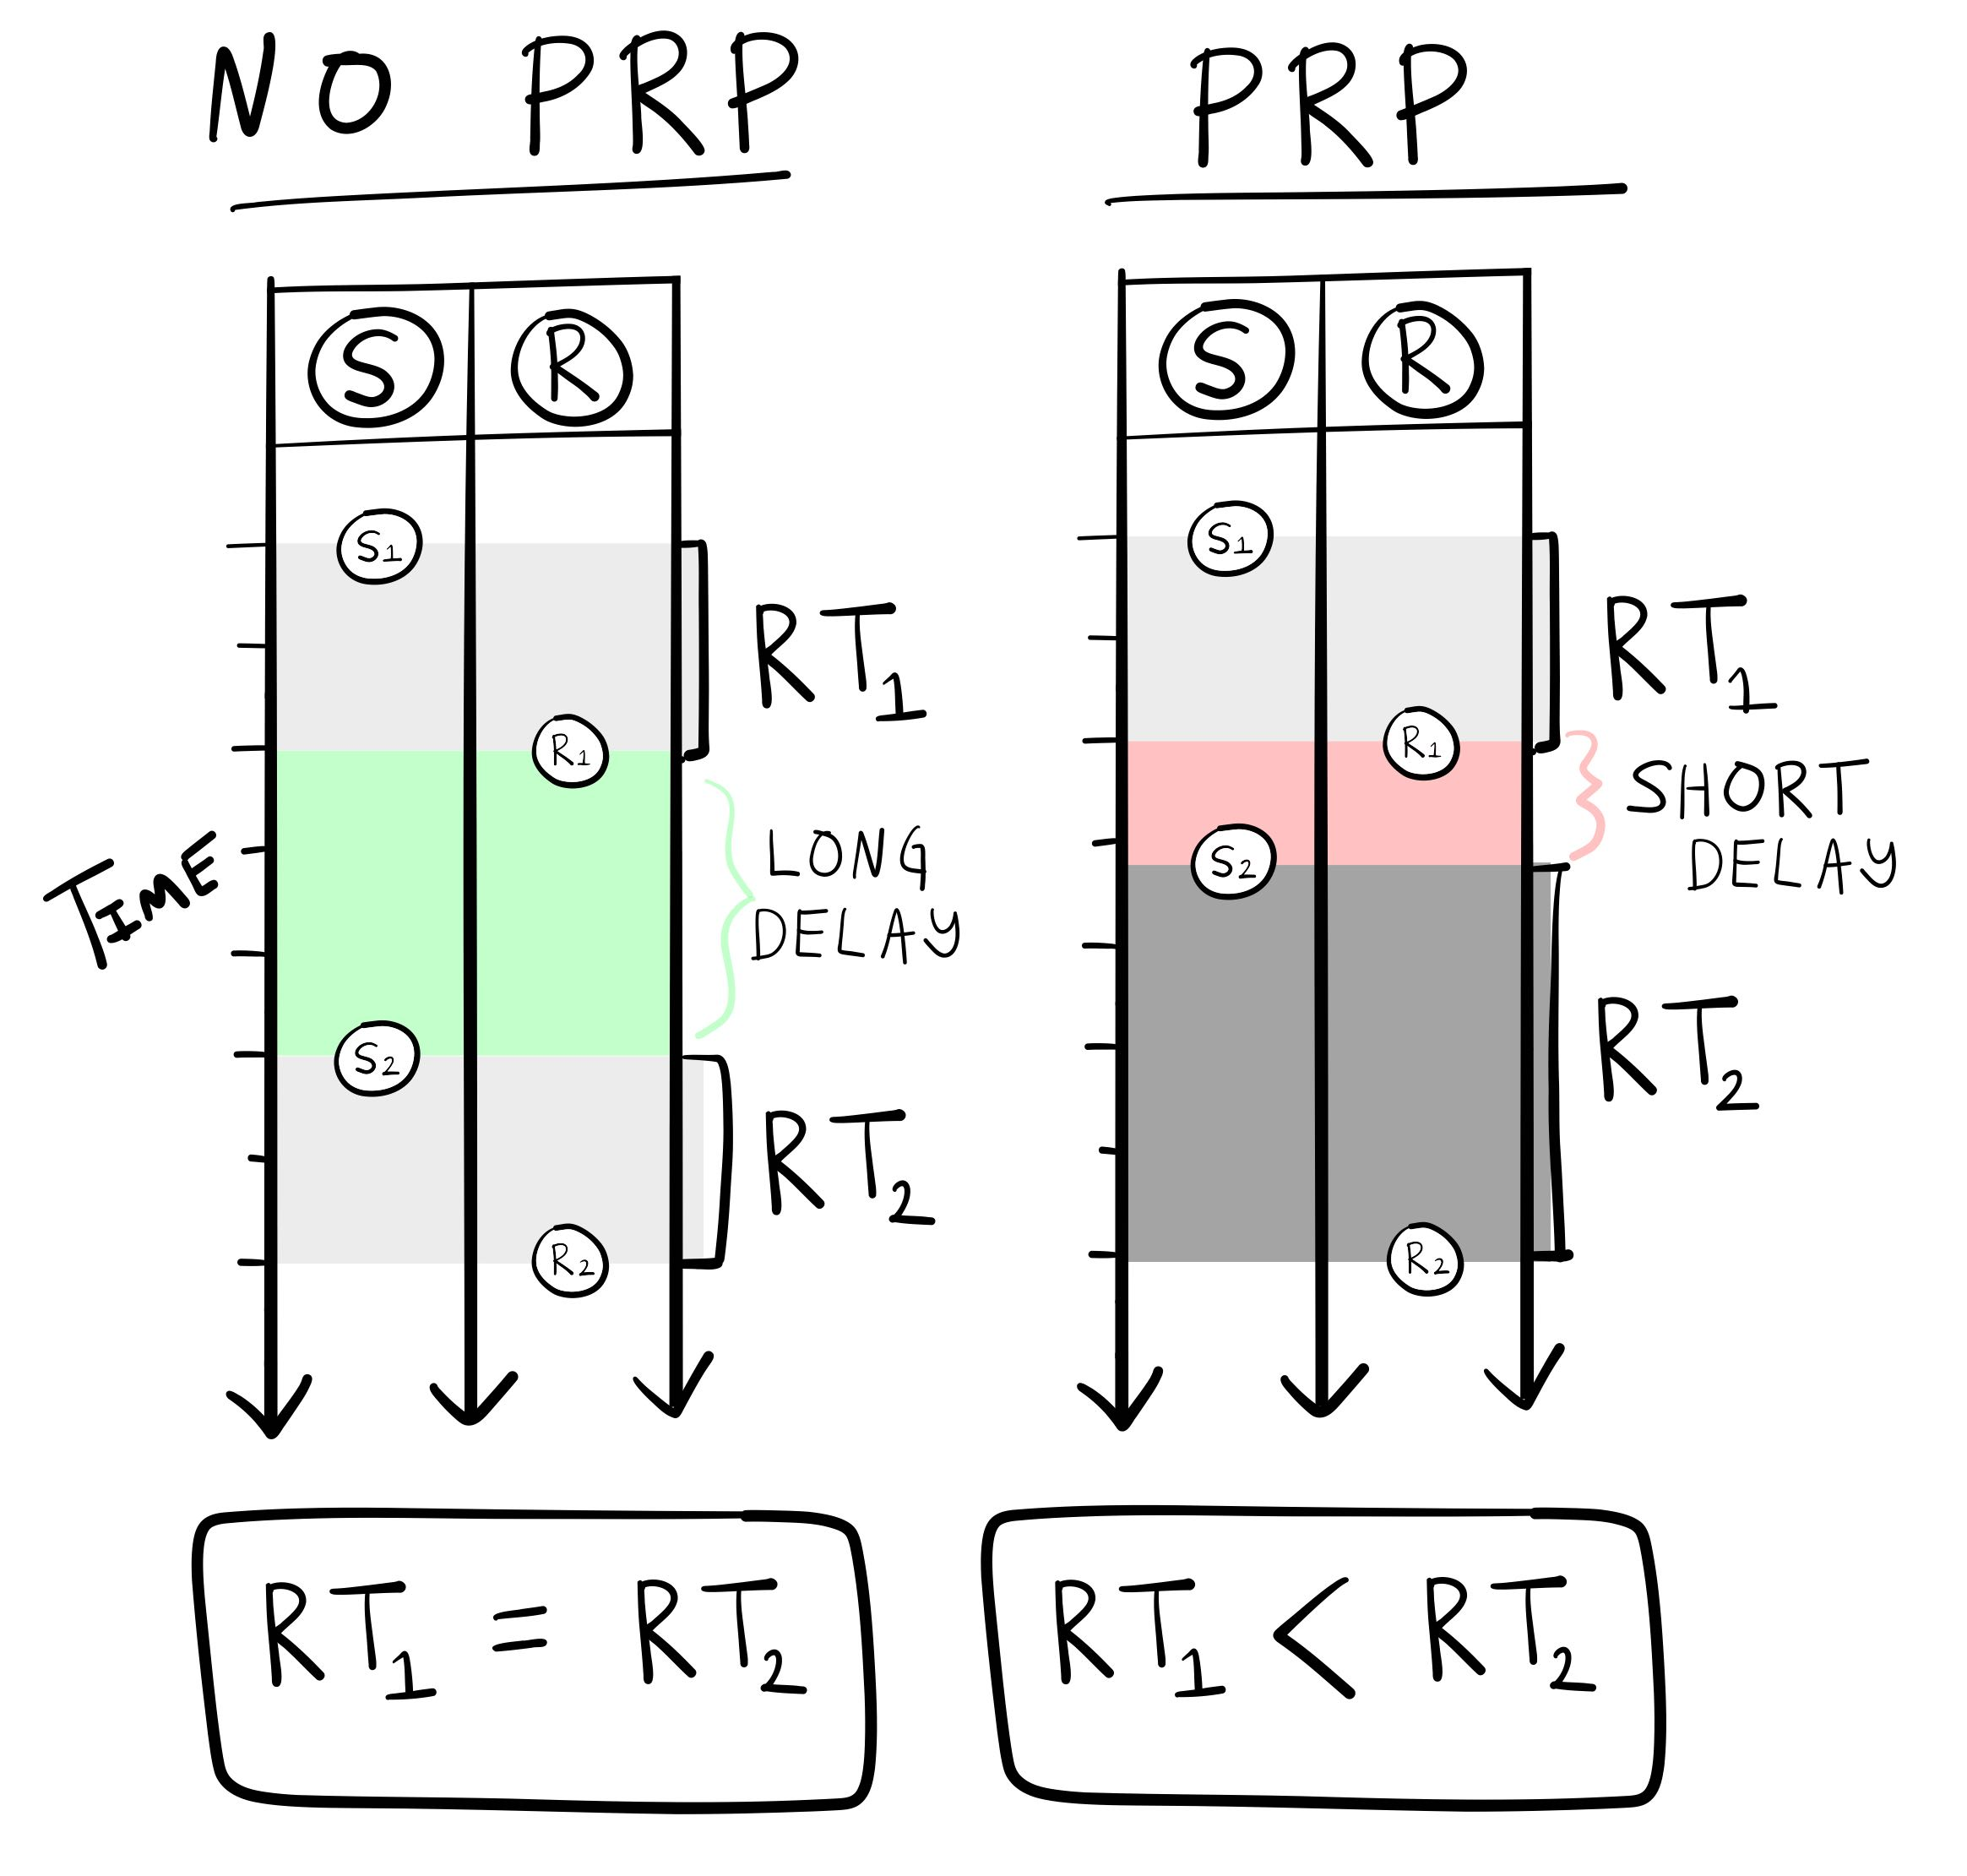
\includegraphics[width=1\linewidth]{imgs/PRP_effect}

\end{floatright50}

The conditions to observe the PRP effect are depicted on the right. In the task, participants are presented with stimuli (S) one after the other, and they asked to response (R) as fast as possible to each of them (e.g., by pressing a button). The long-delay condition highlights an important difference between two successive stimuli. In this case, the second stimulus (\(S_2\)) appears after a long temporal delay following the response (\(R_1\)) to the first stimulus \(S_1\). When this delay is long enough, the average reaction time to the first and second stimulus are generally the same (\(RT_1 = RT_2\)). However, when the delay is shortened, the PRP effect is observed. What happens in performance is that the average reaction time to the second stimulus is longer than the average reaction time to the first stimulus (\(RT_1 < RT_2\)). This lengthening of the second response time is an example of the so-called ``psychological refractory period''.

The PRP effect is a reliable finding in reaction time research, and since Welford hundreds of papers have been published on the phenomena. Note, as we move forward, we will discuss many findings like the PRP effect that have inspired large numbers of research papers. The term \emph{paradigm} is commonly used to refer to collections of research activity that are relatively focused on specific phenomena or tasks. For example, we could refer to the maze-running research discussed last chapter as a paradigm using the task of maze-running. The PRP paradigm is full of papers testing explanations of the PRP phenomena. My purpose in bringing up the PRP literature is not for us to become experts in this one phenomena; instead, the PRP effect provides a clear example of the metaphorical use of processing stages to provide a quasi-mechanical explanation of the phenomena.

So, why does the PRP effect occur? Why is the second response time lengthened if the second stimulus is presented shortly after a previous response? In 1959, Welford described five different theoretical accounts. One possibility was a physical explanation in terms of limitations of signalling among nerve fibers. Another theory had to do with preparedness or expectancy, maybe the shorter duration caused people to be more surprised, and it was the surprise that lengthened the second response. The fifth hypothesis involved a \emph{central mechanism with a single-channel of limited capacity}, and was summarized as follows:\footnote{\protect\hyperlink{ref-welfordEvidenceSinglechannelDecision1959}{A. T. Welford, 1959}.}

\begin{quote}
``In its bare essentials this theory assumes, firstly, a number of sensory input mechanisms each capable of receiving data and storing it for a limited period so that, for example, a short series of signals can be received as a unit. Secondly, it assumes a number of effector mechanisms containing both central and peripheral elements and capable of carrying out a series of actions such as the pressing and release of a key or a series of taps (Vince, 1949) as a single unit. Thirdly, between these two it postulates a single-channel decision mechanism. This is regarded as being of limited capacity in the sense that it takes a finite time to process information and can thus only deal with a limited amount of information in a given time.''
\end{quote}

The mechanism being proposed was like the processing stages of a serial assembly-line. A stimulus is first processed in the perceptual stage, and then moved to the next central processing stage. The central processing stage produces the decision to make a response to the stimulus. This decision is sent to a response production stage, and the response is made. Furthermore, the central processing stage was claimed to be ``capacity limited''. For example, what if it could only deal with one decision at a time? This would create a \emph{bottleneck} in performance. If a second stimulus entered the central stage it would have to \emph{wait in line} until the decision to respond to the first stimulus was sent to the next stage.

Welford and others (Craik,\footnote{\protect\hyperlink{ref-craikTheoryHumanOperator1948}{Craik, K. J. W. (1948). Theory of the human operator in control systems {II}. {Man} as an element in a control system. \emph{British Journal of Psychology}, \emph{38}, 142--148}.} Hick,\footnote{\protect\hyperlink{ref-hickDiscontinuousFunctioningHuman1948}{Hick, W. E. (1948). The discontinuous functioning of the human operator in pursuit tasks. \emph{Quarterly Journal of Experimental Psychology}, \emph{1}(1), 36--51. \url{https://doi.org/d4pnsh}}.} Davis,\footnote{\protect\hyperlink{ref-davisHumanOperatorSingle1957}{Davis, R. (1957). The human operator as a single channel information system. \emph{Quarterly Journal of Experimental Psychology}, \emph{9}(3), 119--129. \url{https://doi.org/d2n3mw}}.} Fraisse,\footnote{\protect\hyperlink{ref-fraissePeriodeRefractairePsychologique1957}{Fraisse, P. (1957). La période réfractaire psychologique. \emph{L'Année Psychologique}, \emph{57}(2), 315--328. \url{https://doi.org/dtnd4s}}.} and Broadbent Broadbent, D. E.\footnote{\protect\hyperlink{ref-broadbentPerceptionCommunication1958}{(1958). \emph{Perception and communication}. {Elsevier}}.}) were part of a new wave of researchers applying recent concepts from telecommunications science and technology to human cognition. For example, the concept of a single-channel decision mechanism that processed information in a capacity limited manner was inspired by telephone technology. The remaining half of this chapter elaborates on the metaphor how it informed the concept of information processing in cognition.

\hypertarget{cybernetics-and-the-macy-conferences}{%
\section{Cybernetics and the Macy Conferences}\label{cybernetics-and-the-macy-conferences}}

If you noticed, we've been jumping around a little bit in historical time. Last chapter we ended with Skinner circa 1938, and this chapter we went back to the time of Donders (circa 1868), and forward in time to the Attention and Performance conference of 1968. That leaves roughly a 30 year gap between 1938 and 1968 that we didn't talk much about. This was a dense historical period that greatly informed the formation of the cognitive sciences. Among other things, there was another world war, the invention of nuclear weapons, the invention of digital computers, and the gradual transition in American psychology from behaviorism to cognitivism. This time period was also home to the Macy Conferences and Cybernetics, which provide a useful perspective on the transitional period.

\href{https://en.wikipedia.org/wiki/Macy_conferences}{The Macy conferences} were held (160 over 19 years) in New York between 1941 and 1960. These conferences were sponsored by the \href{https://en.wikipedia.org/wiki/Josiah_Macy_Jr._Foundation}{Josiah Macy J. Foundation} and involved attendees from a wide variety of academic backgrounds to encourage interdisciplinary interactions and exchange of ideas. For example, many attendees were academics from the disparate fields of psychology, philosophy, anthropology, physiology, linguistics, genetics, and math and computer science (and others). And, rather than discussing specialty topics of little relevance to other fields, they were interested in discussing potential overlaps and bigger issues require sharing and integration of methods between fields.
Many of these exchanges revolved around a movement called \href{https://en.wikipedia.org/wiki/Cybernetics}{cybernetics}. Cybernetics still exists as a field, but is also recognized as the beginning of what is now called the cognitive sciences. Cybernetics also played a transitional role in American psychology by bridging elements of behaviorism with later cognitivism.

\href{https://en.wikipedia.org/wiki/Norbert_Wiener}{Norbert Weiner} is the father of cybernetics, a trans-disciplinary approach concerned with ``control and communication in the animal and the machine.''\footnote{\protect\hyperlink{ref-wienerCyberneticsControlCommunication1948}{Wiener, N. (1948). \emph{Cybernetics or {Control} and {Communication} in the {Animal} and the {Machine}}. {MIT press}}.} Mathematician \href{https://en.wikipedia.org/wiki/Andrey_Kolmogorov}{A. K. Kolmogorov}, cybernetics was ``concerned with the study of systems of any nature which are capable of receiving, storing and processing information so as to use it for control.''\footnote{See also many more definitions of cybernetics in \protect\hyperlink{ref-umplebyDefinitionsCybernetics2008}{Umpleby, S. (2008). Definitions of cybernetics. \emph{The Larry Richards Reader 1997--2007}, 9--11}.}

In Kolmogorov's sense, Skinner's behaviorism was an example of cybernetics with some important missing elements-- he was studying principles of behavioral control in an animal system, but he was not too concerned about internal processes that might be responsible for receiving, storing, and processing information. Cybernetics had a much broader vision of control, which was to understand the principles of any type system that appeared to regulate itself, including humans, animals, and even machines. The hope was that the principles would be somewhat generalizable across systems and allow insights from area to foster innovations in another. For example, if principles of cognitive processing in humans could be better understood, then perhaps machines could be made to operate by those principles, which could lead to artificial forms of intelligence. Thus, sharing findings and methods between domains was encouraged because of the potential for new and unexpected insights.

In other words, cybernetics was OK with psychologists exploring mechanistic metaphors for cognitive processing. For example, from a cybernetics perspective, a psychologist might benefit from learning something about telecommunications technology because those methods could provide a model system for understanding something about how people communicate. Whatever insights were extracted could in turn be useful for understanding communication in other systems, like animals, machines, or other networks using a communication concept. Indeed, major advancements in telecommunication technology were being discussed at the Macy conferences, and the attending psychologists were very quick to to apply those advancements to an emerging cognitive psychology. One of the major advancements was Claude Shannon's ``Information Theory'', which is described first, followed by two ways that it was applied as a metaphor for cognition.

\hypertarget{shannons-information-theory}{%
\section{Shannon's Information Theory}\label{shannons-information-theory}}

There were numerous attendees at the cybernetics conferences whose contributions to the cybernetics movement were also foundational for the cognitive sciences. Most relevant for our current purposes was the American mathematician \href{https://en.wikipedia.org/wiki/Claude_Shannon}{Claude Shannon} (1916 -- 2001). His 1937, master's degree (MIT) was titled ``A Symbolic Analysis of Relay and Switching Circuits.''\footnote{\protect\hyperlink{ref-shannonSymbolicAnalysisRelay1938}{Shannon, Claude E. (1938). A symbolic analysis of relay and switching circuits. \emph{Electrical Engineering}, \emph{57}(12), 713--723. \url{https://doi.org/ggztcn}}.} This was a theoretical paper about the math and logic behind the telephone exchange networks of the day. The exchanges had been automated so that they no longer required a human operator to connect one phone to another, and Shannon's analysis suggested more efficient designs for switches making the connections. The very same math would later be fundamental for the design of circuits in digital computers. In 1940 Shannon completed his Ph.D.~titled, ``An Algebra for Theoretical Genetics''\footnote{\protect\hyperlink{ref-shannonAlgebraTheoreticalGenetics1940}{Shannon, Claude Elwood. (1940). \emph{An algebra for theoretical genetics} {[}PhD Thesis{]}. {Massachusetts Institute of Technology}}.} based on his work at the Eugenic Record Office at Cold Springs Harbor Laboratory. During world war II, he worked at Bell lab's on ``A mathematical theory of cryptography'', which involved methods to send and receive messages on communication lines that might have many other listeners besides the intended recipient. Then, in 1948-49 he published what is now called ``Information theory'' in his book ``The Mathematical theory of communication.''\footnote{\protect\hyperlink{ref-shannonMathematicalTheoryCommunication1949}{Shannon, Claude E., \& Weaver, W. (1949). \emph{The mathematical theory of communication}. {University of Illinois press}. \url{https://books.google.com/books?hl=en\&lr=\&id=IZ77BwAAQBAJ\&oi=fnd\&pg=PP1\&dq=related:neNAI2dkLQcJ:scholar.google.com/\&ots=hknDdVuK4v\&sig=8pbhXsHmouktq7OVKrUO4KLT2NQ}}.}

Information Theory was not developed as a theory for cognition or psychology. It offers a way to mathematically describe general elements of communication systems, and found useful applications in many domains including psychology. We will focus on two ideas from information theory that became popular in early cognitive research. These are the concept of an information channel, and the idea that information can be measured and quantified using Shannon's formula for entropy (\(H\)).

\hypertarget{information-channels}{%
\subsection{Information channels}\label{information-channels}}

An information channel has three major parts-- a sender, a channel, and a receiver--and two big questions, how much information was sent? And, how much was received?

\begin{center}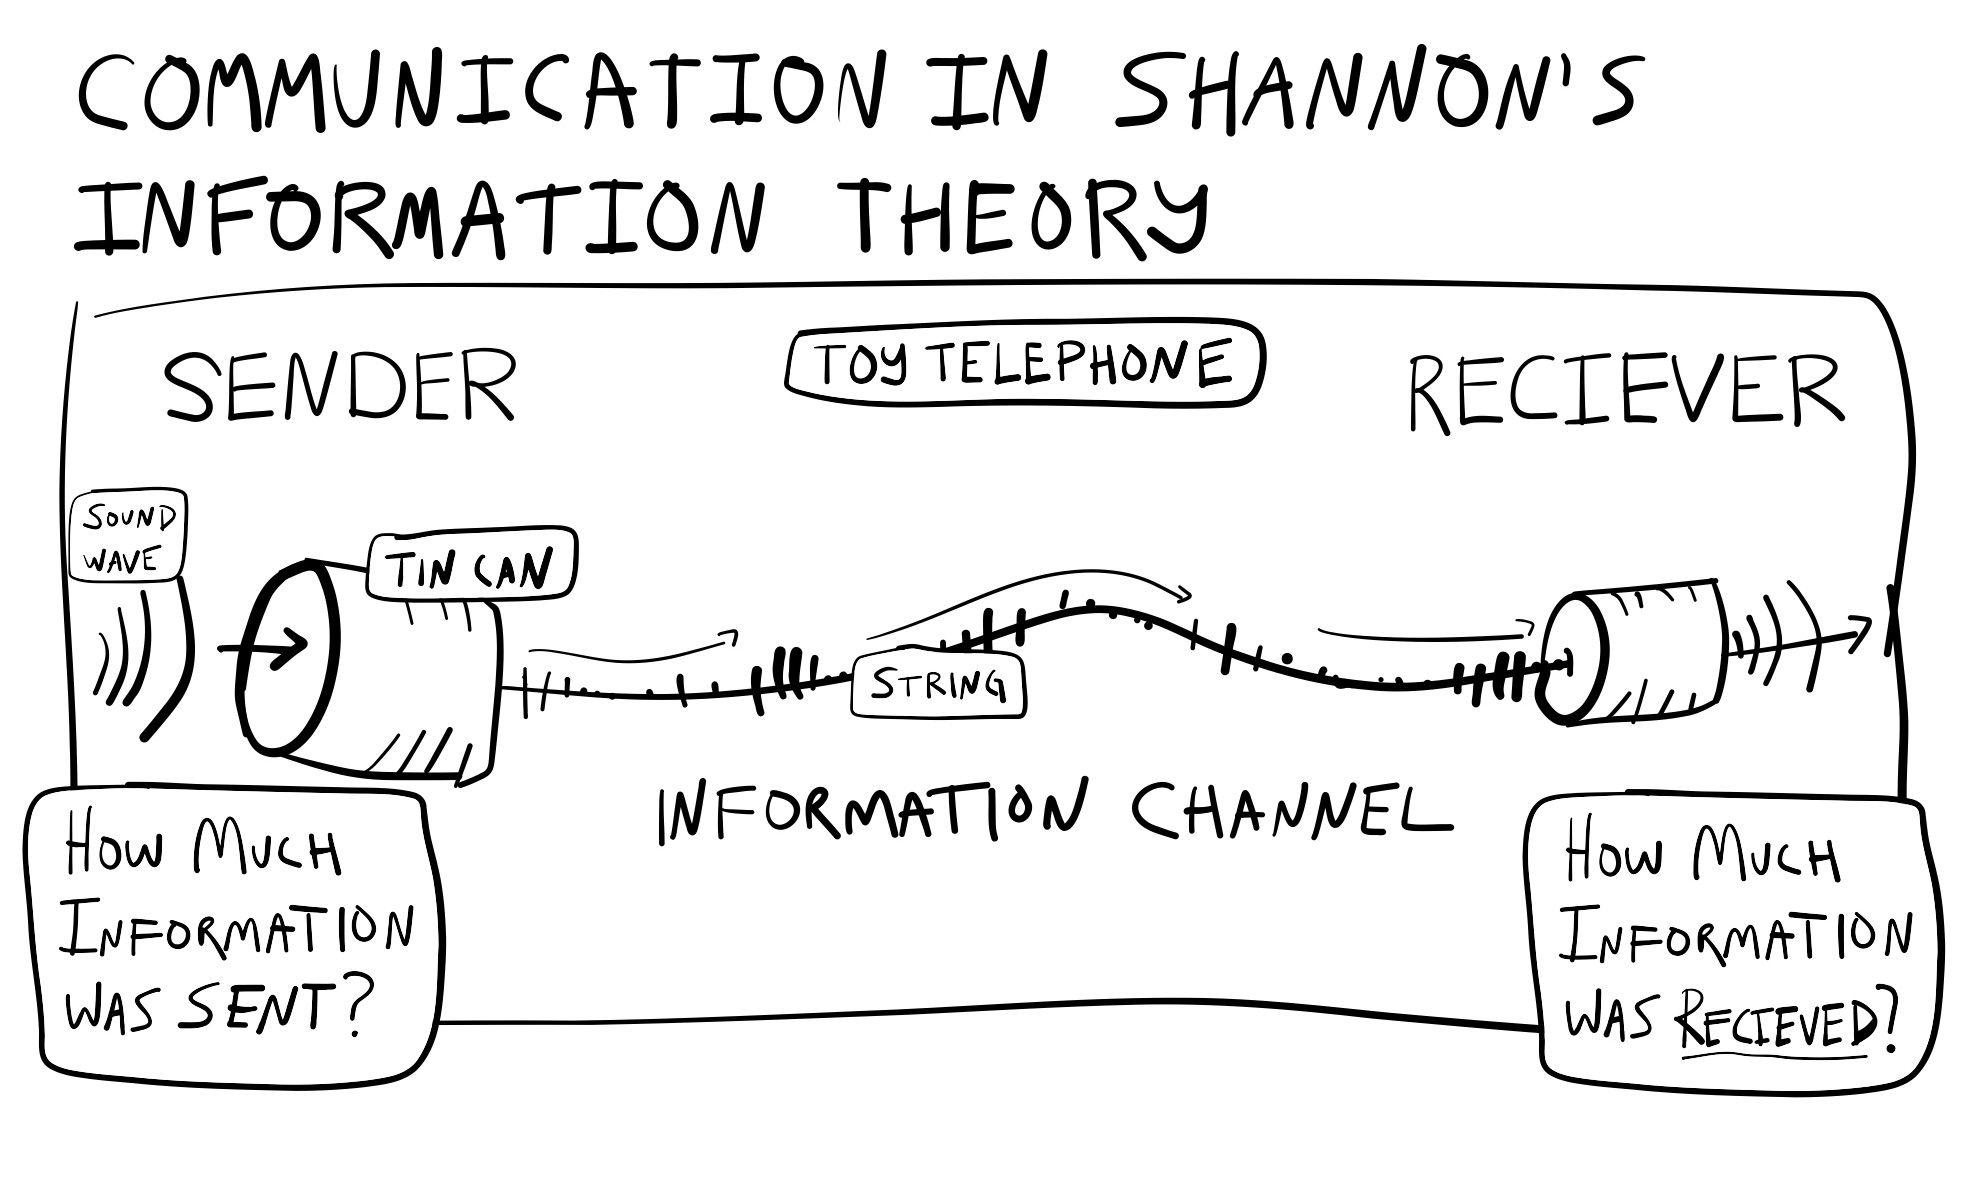
\includegraphics[width=1\linewidth]{imgs/Shannon_info_channel} \end{center}

A toy telephone system made out of tin cans and string is a great example of a simple information channel. In this system, one person speaks into a tin-can on one end. There is a hole in the bottom of the can, and a knot is securely blocking the hole so that the remaining length of string can be unrolled for a distance and connected to another tin can. The person on the other end is holding the second can up to their ears, and listening to the message from the sender. If you have never made this toy, it's just that simple, and it works.

The speaker's vocal chords push air through their mouth creating air-waves in the range of audible frequencies. The waves project into the can and through a process of physical resonance the wave pattern in the air is transferred to the can, which begins to wave with similar frequencies. The can is connected to the string which starts waving in the same way, carrying the wave across the string to the other can. Now the other can starts to wave too, which shapes the air in the can and causes new-air waves to be emitted. These air-waves travel through the air into the ear canal of the person listening on the other end. The outer, middle, and inner then begin vibrating as well and transduce the mechanical waves into nerve impulses, and eventually the receiver listens to the message, and maybe says something back, repeating the process.

Acts of cognition are important bookends to this story. From the beginning we can ask how it is that someone can speak a message at all (or pick up a can, or make a toy telephone), and at the end we can ask how someone hears and understands a message, and decides to respond to it or not. However, for our immediate purposes we will not focus on those psychological aspects, but instead return to some of the questions about the information channel, which is the medium through which the message passes.

An information channel is a general concept with an important property called capacity. An information channel could be a tin-can telephone with a real string connecting two devices, or it could be a wireless cell-phone connected through more advanced technology involving very high frequency waves. Both kinds of phones have a limited ability to send signals, this is called the channel capacity. For example, you can hook up one can to another and hear someone speak on the other end. In loose terms, we could say a string has the capacity to support one message. However, if you hook up more cans to the same string, and allow many people to take at once, the quality of the signal at the receiving end will become increasingly worse. In this sense, the string has a limited amount of capacity to transmit a signal.

Questions about information capacity were fundamental for improving telecommunications technology. For example, what was the information capacity of a physical telephone line, how many calls could it support? What happens when the capacity is exceeded? How could the systems be improved to increase the capacity and support more calls? Could the lines support other kinds of signals? How much? What other kinds of signals?

So far I have used the word information to describe the signal transmitted from a sender to a receiver. The channel that transmits the signal is called the information channel, and we now have the idea that the channel could be limited in capacity. So, an information channel can only transmit a limited amount of information. A really basic next question is\ldots how much?

\hypertarget{measuring-information-h}{%
\subsection{Measuring Information: H}\label{measuring-information-h}}

One of Shannon's mathematical contributions was to propose a definition for quantifying the amount of information. His formula defines information in terms of entropy, or the amount of uncertainty in a system of messages, and is called Shannon's H:

\(H(X) = -1*\sum_\text{i=1}^n P(x_i) * log_2 P(x_i)\)

I will explain what this formula means in a moment. For Shannon's communication theory, it had several useful properties. A formula for quantifying information meant that capacity limitations of information channels could be measured and assigned a value indicating how much information they could carry. Additionally, the content of signals could be analyzed and described in terms of how much information was contained in the signal. Finally, when signals are sent across an information channel and received at the other end, sometimes parts of the signal are lost during transmission. The amount of information lost could now be described and accounted for with Shannons's H.

Shannon's formula defines information in terms of the predictability of a sequence of messages. This is subtly different from the amount of things in a message. For example, if you are asking yourself what does ``information'' mean in everyday usage, you might think about books, websites, or videos that are sources of information. If we are using the number of things to measure the amount of information, then we might say that long books have more information than short books because long books have more words, and thus convey more information in that sense. Shannon emphasizes a different aspect of information in his definition. For example, imagine a really long book with 1,000 pages, but the only word printed in it is the letter ``A'' as many times as possible on every page. Shannon's formula would say this book transmits zero information because the message is 100\% predictable. If you imagine the book as ``sending out a message'', and then ask how much \textbf{new} information is obtained from reading the book, the answer could be zero. For example, I imagine a book-reviewer saying they didn't bother reading it because they already knew it was full of \emph{A}s. In Shannon's theory, communication of information does not occur if the receiver already knows the content of the message.

By contrast, according to Shannon's definition, the amount of information in a message increases as it becomes more unpredictable. For example, a short book could contain many sentences with words in new combinations that you had never encountered before. When you read the book, you find almost every new statement to be unexpected and surprising. According to Shannon, this kind of book contains much more information than the book of As, which has a long message that is entirely expected.

Shannon's definition also takes the definition of information to an oddly extreme place. By definition more random messages have more information,and the ultimate message carrying the most possible information is total randomness \footnote{this is also why H refers to entropy, which is a physics concept for randomness or disorder in a system}. One way to conceptualize this is to think of total randomness as containing all possible messages in a system. For example, consider Borel's (1913) infinite monkey theorem,\footnote{\protect\hyperlink{ref-borelMecaniqueStatiqueIrreversibilite1913}{Borel, É. (1913). La mécanique statique et l'irréversibilité. \emph{J. Phys. Theor. Appl.}, \emph{3}(1), 189--196. \url{https://doi.org/c9nnbz}}.} which says that a room full of monkeys typing letters on a keyboard for infinity will eventually produce any text, even the works of Shakespeare. So, even though most of the books written by the typing monkeys will be totally incoherent, they are producing all of the possible ways to print letters in books, so in that sense that they are writing all of the books that make sense, and all of the ones that don't \footnote{as in Borges \href{https://en.wikipedia.org/wiki/The_Library_of_Babel}{Library of Babel}}, which according to Shannon, is a lot of information.

I bring up this last example so you do not equate Shannon's definition of information with the meaningfulness of the stimulus. As we dive into the formula next, we will see it is just a single number to describe the amount of randomness in a system. If the system was a coin that could transmit one of two messages--heads or tails--then, Shannon's H is simply a measure of how fair or biased the coin is. A fair coin is completely random, and transmits the maximal amount of information. A biased coin comes up heads or tails more often, is more predictable, and transmits less information.

\hypertarget{computing-h}{%
\subsection{Computing H}\label{computing-h}}

Let's use the coin flipping example to compute H, or the amount of information according to Shannon's formula. Here is the formula again:

\(H(X) = -1*\sum_\text{i=1}^n P(x_i) * log_2 P(x_i)\)

The capital X refers to the set of discrete events that can occur in a series of messages. In a coin toss there are two events, heads or tails. The term \(P(x_i)\) refers to the probability that each event occurs, and \(log_2 P(x_i)\) refers to taking the logarithm base 2 of that same probability. To state what the formula says in a sentence: multiply (\(*\)) the probability of an event (\(P(x_i)\)) by it's logarithm base 2 and find the product, do the same for all events (from i= 1 to n, the number of events), add all of the products up (\(\sum_\text{i=1}^n\)), and then multiply the final sum by -1.

The table below shows the calculation of H for a fair coin. A fair coin has two possible events, heads or tails, and each event has the same .5 probability of occurring.

\begin{tabular}{l|l|l|l|l}
\hline
Events & $i$ & $P(x_i)$ & $log_2 P(x_i)$ & $P(x_i)*log_2 P(x_i)$\\
\hline
Heads & 1 & 0.5 & -1 & -0.5\\
\hline
Tails & 2 & 0.5 & -1 & -0.5\\
\hline
sum &  &  & $\sum_\text{i=1}^n$ & -1\\
\hline
H &  &  & $-1*\sum_\text{i=1}^n$ & 1\\
\hline
\end{tabular}

To walk through the table, in the first row we have the calculations for heads. The probability of heads is .5.

\(P(x_i) = .5\)

The logarithm base 2 of .5 is -1.

\(log_2 P(x_i = .5) = -1\)

Multiplying the two together gives -.5.

\(P(x_i)*log_2 P(x_i) = .5 * -1 = -.5\)

In row two, we see the same calculations because the probability of tails is also .5. The last steps of the formula involve summing up the products in the last column.

\(\sum=-.5 + -.5 = -1\)

Finally to convert to a positive number, the sum is multiplied by a -1, (-1 * -1 = 1). So, for a fair coin, \(H = 1\).

\hypertarget{bits-of-information}{%
\subsection{Bits of information}\label{bits-of-information}}

Shannon's formula uses a base 2 logarithm which produces a number in the unit of \href{https://en.wikipedia.org/wiki/Bit}{bits}. If you are not familiar with bits, they are the building blocks of modern digital computers. One bit represents a single binary operator that can take on one of two possible states. For example, a coin could represent a bit. If we stipulated that a coin could only land heads or tails, then it would function the same as a binary operator with two possible states. Other kinds of binary operators include logic, where a logical statement can be either TRUE or FALSE. It is also possible to express numbers using binary symbols. In this case, numbers are represented with only two symbols 0 or 1.

Bits can be used to measure the total number of discrete events in a system of messages. Let's see how.

A single bit has two states, 0 or 1. So, we could use a single bit to represent two unique states, like heads or tails.

How many states can two bits represent? This would involve counting all of the unique ways of combining the states from two bits, for example, the first and second bit could be 0 (00), the first bit could be zero and the second a one (01), and so on. All of four possibilities are: 00, 01, 10, and 11. The figure below shows the relationship between number of bits, and the number of unique events that can be represented by combining bits together.

\begin{center}\includegraphics[width=1\linewidth]{imgs/Shannon_bits} \end{center}

The relationship between number of bits and number of unique events they can code is defined by raising 2 to the number of \(Bits\):

\(2^\text{Bits} = \text{number of events}\)

The figure shows some examples of computing the number of unique combinations that can be coded with up to three bits.

\hypertarget{h-bits-predictability-and-information}{%
\subsection{H, Bits, predictability and Information}\label{h-bits-predictability-and-information}}

Let's put all of these concepts together in thinking about a set of messages in Shannon's communication system. Remember, a sender sends a message to a received across an information channel. In this system and important question is how much information is in the message? How much capacity to transmit information does the channel have? And, how much information is received or lost in transmission? Shannon's formula provides a way to calculate answers to these questions; however, in order to do the calculations the message needs to be converted into discrete events so that it can be measured in terms of bits.

Let's consider a simple communication system where a sender can only send one of four events: A, B, C, or D. How many bits are needed to represent these four events? From the figure above we can see that the answer is four bits.

If a sender is communicating only discrete events like As, Bs, Cs, and Ds, then Shannon's formula provides a way to measure the amount of uncertainty in the message.

The most uncertainty occurs when the message is completely random. By definition, this means that the sender randomly chooses to send As, Bs, Cs, and Ds with equal probability. This is like a four-sided coin flip (if that was possible). Each of the probabilities is .25, or 1/4. In this situation, the receiver has no way of predicting which event will occur as they receive the message. It is maximally uncertain. Watch what happens when we compute H using Shannon's formula, we compute \(H = 2\), which is the same as the number of bits needed to represent each of the four events:

\begin{tabular}{l|l|l|l|l}
\hline
Events & $i$ & $P(x_i)$ & $log_2 P(x_i)$ & $P(x_i)*log_2 P(x_i)$\\
\hline
A & 1 & 0.25 & -2 & -0.5\\
\hline
B & 2 & 0.25 & -2 & -0.5\\
\hline
C & 3 & 0.25 & -2 & -0.5\\
\hline
D & 4 & 0.25 & -2 & -0.5\\
\hline
sum &  &  & $\sum_\text{i=1}^n$ & -2\\
\hline
H &  &  & $-1*\sum_\text{i=1}^n$ & 2\\
\hline
\end{tabular}

We have just seen that when a communication involves a maximally unpredictable set of events, Shannon's formula for H returns the number of bits needed to represent each of the unique events in the message. In other words, the number of bits represents an upper bound on the amount of information in a message, in this case it represents maximal uncertainty when the events occur with equal probability.

What if the events do not occur with equal probability? This would mean that some of the events are more likely than others. In Shannon's system, whenever some events are more likely than others something special happens at the receiving end of the message. The receiver is now able to predict some of the message. For example, if the message 70\% As, 10\% Bs, 10\% Cs, and 10\% Ds, the receiver would be able to predict that each event has a high probability of being an A, and a low probability of being a B, C, or D. Let's enter this situation into the formula for H and see what happens:

\begin{tabular}{l|l|l|l|l}
\hline
Events & $i$ & $P(x_i)$ & $log_2 P(x_i)$ & $P(x_i)*log_2 P(x_i)$\\
\hline
A & 1 & 0.7 & -0.514573172829758 & -0.360201220980831\\
\hline
B & 2 & 0.1 & -3.32192809488736 & -0.332192809488736\\
\hline
C & 3 & 0.1 & -3.32192809488736 & -0.332192809488736\\
\hline
D & 4 & 0.1 & -3.32192809488736 & -0.332192809488736\\
\hline
sum &  &  & $\sum_\text{i=1}^n$ & -1.35677964944704\\
\hline
H &  &  & $-1*\sum_\text{i=1}^n$ & 1.35677964944704\\
\hline
\end{tabular}

In this case, H is computed as 1.35, which means that events in the message require less than 2 bits. There are still four events, but one of them is more predictable then the others. If we made one of the events even more predictable (e.g., like A = .97), then the amount of bits needed would decrease and get closer to zero.

\begin{tabular}{l|l|l|l|l}
\hline
Events & $i$ & $P(x_i)$ & $log_2 P(x_i)$ & $P(x_i)*log_2 P(x_i)$\\
\hline
A & 1 & 0.97 & -0.0439433475875971 & -0.0426250471599691\\
\hline
B & 2 & 0.01 & -6.64385618977472 & -0.0664385618977472\\
\hline
C & 3 & 0.01 & -6.64385618977472 & -0.0664385618977472\\
\hline
D & 4 & 0.01 & -6.64385618977472 & -0.0664385618977472\\
\hline
sum &  &  & $\sum_\text{i=1}^n$ & -0.241940732853211\\
\hline
H &  &  & $-1*\sum_\text{i=1}^n$ & 0.241940732853211\\
\hline
\end{tabular}

If one of the event occurs 100\% of the time, and the others occur 0\% of the time, then H=0. What happens in the formula is that \(log2(1) = 0\), and \(log2(0)= -infinity\). By convention, the negative infinities are turned into 0s, which results in a sum of 0s, such that \(H=0\).

\begin{tabular}{l|l|l|l|l}
\hline
Events & $i$ & $P(x_i)$ & $log_2 P(x_i)$ & $P(x_i)*log_2 P(x_i)$\\
\hline
A & 1 & 1 & 0 & 0\\
\hline
B & 2 & 0 & -Inf & 0\\
\hline
C & 3 & 0 & -Inf & 0\\
\hline
D & 4 & 0 & -Inf & 0\\
\hline
sum &  &  & $\sum_\text{i=1}^n$ & 0\\
\hline
H &  &  & $-1*\sum_\text{i=1}^n$ & 0\\
\hline
\end{tabular}

\hypertarget{summary-1}{%
\subsection{Summary}\label{summary-1}}

In the next sections we will see examples of how Shannon's information theory was applied in psychology. To summarize the preceding sections, here is what we have learned.

Shannon characterized communication as involving an information channel that transmits discrete messages from a sender to a receiver. He measured the amount of information transmitted in terms of bits. Messages with more unpredictable events transmit more information, measured in bits, than messages with more predictable events. A message that contains 100\% predictable events transmits no information because the receiver does not need to receive the message to know what the contents are. A message that is 100\% random transmits the maximal amount of information, because the receiver is unable to predict the events, and ``learns'' something new about the message every time. Messages with intermediate levels of predictability transmit an intermediate amount of information between 0 (maximum predictable) and the number of bits (maximum uncertainty) representing all possible events in the message.

\hypertarget{hick-hyman-law}{%
\section{Hick-Hyman ``Law''}\label{hick-hyman-law}}

Let's connect back to two previous issues. First, we have been discussing mechanistic metaphors of cognition. Shannon's ideas about communication along an information channel were applied as metaphors that had potential to provide insight cognitive processes. Second, in our previous discussions of research we saw examples of reaction time methods. This section discusses the Hick-Hyman ``Law'', which was a very promising application of information theory to findings in the study of choice reaction-times. The word ``Law'' is quoted because the findings are referred to this way in the literature, but there are edge-cases where the law does not always hold up.

\hypertarget{choice-reaction-time}{%
\subsection{Choice Reaction time}\label{choice-reaction-time}}

A basic choice reaction time (CRT) task was already described in the Donders section. Here it is again. In a choice reaction study a participant is presented with one stimulus per trial, and instructed to identify the stimulus as quickly and accurately as possible by making a unique response to the stimulus. For example, the stimulus could be an X or an O, and the response could be to say ``X'' out loud (when an X is presented), or to say ``O'' out loud (when an O is presented). The response could be made in different ways too. For example, the buttons on a computer keyboard are often used in reaction time studies, so the ``X'' on a keyboard could be used to respond to an X, and the ``O'' on a keyboard could be used to respond to an O.

There are many variations on the general choice reaction time procedure. For example, if you were the experimenter, you could manipulate the kind of stimuli presented, the number of trials, the number of times a stimulus is presented, the kind of response made to each stimulus. You could make the stimuli more difficult to identify by degrading them, you could make the responses easier or harder to make by making the required movements more or less natural. You could give people more or less practice, and measure how consistent they are over time, or whether they get faster or not. All of these kinds of manipulations and more have been conducted and reported in the choice reaction time literature. As you might imagine, this research enterprise produces many patterns of data, because it turns out that several factors make reaction times faster or slower.

When researchers are presented with an overwhelming amount of data, they often look for regular patterns in the data. This helps to summarize the data into more manageable and understandable units. This practice of looking for prominent and predictable patterns in data is similar to the process of identifying ``laws'' about a natural phenomena. During the behaviorism period there was interest in discovering laws of behavior, and this same interest applied to research on choice reaction time. For example, a general question was, ``what are the laws governing choice-reaction time?''. What makes choice-RT faster or slower? Before Hick and Hyman came along, prior work had produced one very reliable finding.

\hypertarget{the-number-of-alternatives-increases-choice-rt}{%
\subsection{The number of alternatives increases choice-RT}\label{the-number-of-alternatives-increases-choice-rt}}

The law-like finding was that choice reaction time increased as the number of alternatives increased. For example, in a choice-RT study it is possible to vary the number of unique stimulus-response pairs. A task could have two stimuli and two responses, or four stimuli and four responses, or any number of stimuli and corresponding responses. The set of possible stimulus-response pairs are called the alternatives \footnote{the choice-RT task is also called an N-AFC task, where N specifies the number of alternatives (A) in the forced choice (FC) task.}.

When researchers manipulated the number of alternatives in the task, they found that average response time to respond to any stimulus goes up and up, as the number of alternatives increases.

\hypertarget{number-of-alternatives-or-information-in-the-message}{%
\subsection{Number of alternatives or ``Information'' in the message?}\label{number-of-alternatives-or-information-in-the-message}}

\href{https://en.wikipedia.org/wiki/W._E._Hick}{William E. Hick} (1912 -- 1974) was a British psychologist,\footnote{And member of the British cybernetics ``Ratio club,'' \protect\hyperlink{ref-hollandOriginsBritishCybernetics2011}{Holland, O., \& Husbands, P. (2011). The origins of {British} cybernetics: The {Ratio Club}. \emph{Kybernetes}, \emph{40}(1/2), 110--123. \url{https://doi.org/dn98st}}.} and \href{https://en.wikipedia.org/wiki/Ray_Hyman}{Ray Hyman} an American psychologist, who both had the insight to examine findings in the choice reaction-time literature from the perspective of Shannon's information theory. They both developed experimental methods to test the idea that people might be sensitive to the amount of ``information'' in stimulus set, rather than simply the number of alternatives.

The metaphor was that the experimenter is sending information to the subject over the course of the choice reaction time experiment. One question was whether the subjects' ability to process the message was influenced by the amount of information in the message. Prior research had already shown findings that were consistent with an information theory interpretation.

For example, choice reaction times were faster when there were two alternatives compared to four alternative. Typically, stimuli were presented randomly on each trial. So, from Shannon's information theory, a task with two unpredictable alternatives carried 1 bit of information, but a task with four unpredictable alternatives carried 2 bits of information. The question for Hick and Hyman was whether increasing the number of alternatives (2 vs 4) was slowing people down for some reason, or whether it was really increases to the amount of information (1 bit vs 2 bits) that was slowing people down (perhaps because more information required more processing time). The problem was that the number of alternatives and amount of information in bits was completely confounded in prior experiments. The solution was to conduct new experiments that de-confounded the relationship between number of alternatives and amount of information.

\hypertarget{deconfounding-alternatives-from-information}{%
\subsection{Deconfounding alternatives from information}\label{deconfounding-alternatives-from-information}}

The solution was to create different versions of a choice-reaction time task that independently varied the number alternatives and the amount of information. In this kind of experiment it would be possible to determine whether reaction times were being influenced by the number of alternative, the amount of information, or both.

We have already seen some ways to manipulate the amount of information in a message. One is to change the number of unique alternatives sent in the message, and the other is to change the predictability of each of event in the message. For example, in the preceding section we saw that communication with four equi-probable events (A, B, C, D) required 2 bits of information. However, if one of the events (A) was more probable than the others, the number of bits information was reduced. As a result, it would be possible to have different versions of a choice reaction time task that held the number of alternatives constant (e.g., four), but changed the predictability of the alternatives, which would vary the amount of information in the task.

\hypertarget{the-experiments}{%
\subsection{The experiments}\label{the-experiments}}

Hick published his results in 1952,\footnote{\protect\hyperlink{ref-hickRateGainInformation1952}{Hick, William E. (1952). On the rate of gain of information. \emph{Quarterly Journal of Experimental Psychology}, \emph{4}(1), 11--26. \url{https://doi.org/10.1080/17470215208416600}}.} and Hyman published his in 1953.\footnote{\protect\hyperlink{ref-hymanStimulusInformationDeterminant1953}{Hyman, R. (1953). Stimulus information as a determinant of reaction time. \emph{Journal of Experimental Psychology}, \emph{45}(3), 188--196. \url{https://doi.org/cq3kjd}}.} We will take a quick look at Hyman's experimental conditions and findings.

\hypertarget{experiment-i-hyman-1953}{%
\subsubsection{Experiment I (Hyman 1953)}\label{experiment-i-hyman-1953}}

The first experiment was a choice-reaction time task with 8 different conditions, corresponding to the number of alternatives, from 1 to 8. In each condition, all stimuli were presented randomly. Thus, the amount of bits in each condition was ranged from 0 to 3 (bits for 1 to 8 alternatives are: 0, 1, 1.58, 2, 2,32, 2,58, 2,81, and 3). As others had found, Hyman's subjects showed a strong linear relationship between bits and reaction time. Reaction time increased linearly with amount of bits. Note, however, in Experiment I, the number of alternatives, was completely confounded with the amount of bits.

\hypertarget{experiment-ii-hyman-1953}{%
\subsubsection{Experiment II (Hyman 1953)}\label{experiment-ii-hyman-1953}}

The second experiment varied the amount information in bits and the number of alternatives separately, again across 8 conditions. A table showing the design of each of the 8 conditions is shown below, along with some mark-up to highlight important features of the design.

\begin{center}\includegraphics[width=1\linewidth]{imgs/Hyman_e2} \end{center}

The first two conditions both had 2 alternatives each, however, the choices were more predictable in the first than second condition. In condition 1, the first alternative occurred more often (9/10 times) than the second alternative (1/10 times). In condition 2, the first alternative still occurred more often than the second, but was slightly less predictable (8/10 vs 2/10 times). Using Shannon's formula to calculate the number bits in each condition, Hyman reports .47 bits for condition 1, and .72 bits for condition 2. If reaction times are influenced by the number of alternatives, then they should be the same in condition 1 and 2, because they both had the same number of alternatives (two each). If reaction times are influenced by the amount of information (measured in bits), then they should be slower in condition 2 compared to condition 1, because condition 2 required more bits (it was less predictable).

The table shows six other conditions. Hyman constructed similar conditions for four, six and eight alternatives. For example, conditions 3 vs 5 both had four alternatives, but condition 5 had more bits (1.99) because the individual choices were less predictable. Similarly, conditions 4 and 6 both had six alternatives, but condition six had more bits because it's alternatives were less predictable. Finally, conditions 7 and 8 both had eight alternatives, but condition 8 was more unpredictable than condition 7.

\hypertarget{the-results}{%
\subsubsection{The results}\label{the-results}}

Hyman reported results from four subjects, the graph below shows original results from two of his participants. Note, Hyman had conducted a third experiment where he manipulated the amount of information separately from the number of alternatives in a slightly different way. All told, his subjects had completed three experiments worth of choice reaction time experiments. All of them had different numbers of alternatives, and separately manipulated amounts of information measured in bits. The big finding can be stated by the Hick-Hyman Law: choice-reaction time increased as a linear function of the information (measured in bits) in the stimulus set. Critically, it was not the number of number alternatives that was making people slower, it seemed to the amount of information in the stimulus set.

\begin{center}\includegraphics[width=1\linewidth]{imgs/Hick_hyman_law} \end{center}

\hypertarget{implications-for-behaviorism}{%
\subsection{Implications for Behaviorism}\label{implications-for-behaviorism}}

I could imagine some behaviorists being disturbed by the results of Hick and Hyman's findings. On the one hand, they should have been very impressed because the results appeared so orderly and lawful. Hick and Hyman might have discovered a natural law about humans and stimulus-response processes. Not only were behaviorists interested in stimulus-response processes, the discovery of behavioral laws was of paramount importance to the enterprise of behaviorism.

On the other hand, the problem with the Hick-Hyman law was that it violated ideological aspects of behaviorist assumptions. For example, behaviorists were interested in understanding the lawful regularities connecting a stimulus with a subsequent response. But, consider what Hick and Hyman had shown. Their finding was that a response to a stimulus \textbf{did not depend on the stimulus that was presented}; instead, the speed of responding to the presented stimulus apparently depended \textbf{on the predictability of the other stimuli that could have been presented instead}. In other words, people were not only responding to a stimulus, they were also responding to all the other stimuli that were not presented. Or, we could say that responses to one stimulus were being influenced by expectations about other stimuli in the set of possible stimuli. Thus, the Hick-Hyman law was a complicating factor for theories of behaviorism that were not acknowledging a role for non-presented stimuli and/or expectations about stimuli to influence behavior. Furthermore, the whole information processing metaphor was a step away from behaviorism, because it implied the existence of intervening mental operations between a stimulus and response--and, it came along with a mathematical system in Shannon's communication theory, that could potentially be useful for describing the nature of the mental operations.

\hypertarget{debate-about-interpretation}{%
\subsection{Debate about interpretation}\label{debate-about-interpretation}}

Hick and Hyman were not the only psychologists incorporating information theory into psychology, and their example was chosen to fit with the theme of reaction time measurements in this chapter. The 1950s saw many psychologists relate their observations in terms of information theory. However, the application of information theory to psychology also fell out of favor for several reasons in the 1960s, even though it continued to re-appear throughout the decades, and remains an important tool in modern cognitive research.

\hypertarget{information-theory-was-not-a-psychological-theory}{%
\subsubsection{Information theory was not a psychological theory}\label{information-theory-was-not-a-psychological-theory}}

A primary issue was that ``information theory'' was not a theory of psychological process. It was just simple mathematical formula to summarize the uncertainty (information) in a set of stimuli. It was interesting that reaction times were linearly related to the uncertainty in the stimulus set, but this observation in and of itself did not explain the mechanism. What was causing reaction times to follow the ``information'' in the stimulus set? Information theory did not provide an answer, it just provided a measure.

\hypertarget{the-hick-hyman-law-could-be-violated}{%
\subsubsection{The Hick-Hyman law could be violated}\label{the-hick-hyman-law-could-be-violated}}

The potential discovery of law relating stimulus set information to reaction time performance generated interest among other researchers, and it didn't take very long for the Hick-Hyman law to show some inconsistencies.\footnote{For a review see, \protect\hyperlink{ref-proctorHickLawChoice2018}{Proctor, R. W., \& Schneider, D. W. (2018). Hick's law for choice reaction time: {A} review. \emph{Quarterly Journal of Experimental Psychology}, \emph{71}(6), 1281--1299. \url{https://doi.org/gfs37w}}.}

One example was the role of practice, which leads to performance improvements in most tasks including choice-reaction time tasks. Teichner \& Krebs reviewed the literature on practice effects in 1974,\footnote{\protect\hyperlink{ref-teichnerLawsVisualChoice1974}{Teichner, W. H., \& Krebs, M. J. (1974). Laws of visual choice reaction time. \emph{Psychological Review}, \emph{81}(1), 75. \url{https://doi.org/br3tcg}}.} and suggested that the Hick-Hyman law may not apply for highly practiced subjects. For example, a highly practiced subject would be fast in all conditions, no matter how many alternatives there were. In these cases, reaction-time performance would not depend on the amount of information in the stimulus-set, but instead on factors to do with practice.

Another example was the supposed linear relationship between number of bits and reaction-time. Most studies had used a small range of alternatives (2 - 32, or 1-5 bits). In 1963, Siebel\footnote{\protect\hyperlink{ref-seibelDiscriminationReactionTime1962}{Seibel, R. (1962). Discrimination reaction time as a function of the number of stimulus-response pairs and the self-pacing adjustment of the subject. \emph{Psychological Monographs: General and Applied}, \emph{76}(42), 1. \url{https://doi.org/b9gnjk}}.} created a task that had up to 1032 alternatives, and found that practiced subjects showed very little difference in reaction times compared to a task with 31 alternatives. He suggested the Hick-Hyman Law might only apply to a small range of set-sizes that was common in the literature. But, in 1966, Hilgendorf\footnote{\protect\hyperlink{ref-hillgendorfInformationInputResponse1966}{Hillgendorf, L. (1966). Information input and response time. \emph{Ergonomics}, \emph{9}(1), 31--37. \url{https://doi.org/dd5k9b}}.} used yet another task capable of presenting 1000 alternatives, and found that the Hick-Hyman law did show a linear relationship with reaction time, even across the large range in set-size.

As a whole, the choice reaction time procedure is similar to the PRP paradigm. It has generated hundreds of experiments and idiosyncratic findings, and by now, many different theories and explanations of the results. Below, we consider a few explanations of Hick and Hyman's findings.

\hypertarget{hicks-explanations}{%
\subsubsection{Hick's explanations}\label{hicks-explanations}}

Hick considered four categories of explanations for the finding that reaction times increase as a function of uncertainty in the stimulus set. And, they were all different from the behaviorist approach we saw last chapter. For example, Hick used mechanistic metaphors to describe possible operations that might be taking place in between a stimulus-response, and he considered how these operations might be able to account for his data.

One idea was a match-to-template hypothesis. If a person had to identify a stimulus as being one of four stimuli, they could compare it to mental templates of each of the alternatives, and then they could respond as soon as they matched the current stimulus to one of the templates. If the comparison was conducted in serial (one after the other), then the set-size of alternatives should increase the reaction time. This is because people would, on average, need to make more mental comparisons between a perceived stimulus and the additional mental templates. However, the match-to-template hypothesis would only explain why reaction time would increase as a function of set-size, and not as a function of the uncertainty of the alternatives.

Another idea was that people were somehow using binary logic to aid the task of stimulus identification. For example, a single stimulus from a set could be found by progressively applying binary tests. Consider finding one stimulus from a set of eight by asking binary questions with a yes/no answer. Here it takes three bits, or three binary decisions to identify the stimulus. For example:

\begin{enumerate}
\def\labelenumi{\arabic{enumi}.}
\tightlist
\item
  Is the stimulus in the first four items? Yes (if no, then it must be in the last four. We'll assume it is in the first four)
\item
  Is the stimulus in the first two? No, then it must be in the second two (3rd or 4th item).
\item
  Is the stimulus the 3rd item? Yes, you have found it; or No, it must be the 4th item, and you have found it.
\end{enumerate}

\hypertarget{a-tale-of-two-confounds-priming-explanations}{%
\subsubsection{A tale of two confounds: Priming Explanations}\label{a-tale-of-two-confounds-priming-explanations}}

The Hick-Hyman law came from experiments attempting to de-confound the influence of set-size (number of alternatives) from the possible influence of stimulus uncertainty (information in bits) on choice reaction-time performance. However, the manipulations to hold set-size constant, and vary predictability of the individual stimuli in the set could create new confounds. For example, when you change stimulus probabilities such that some stimuli occur more than others, you may also change the number of immediate repetitions of two successive stimuli.

Another well-known finding in the reaction time literature is called \emph{repetition priming}. For example, if you respond to an \emph{A} stimulus, and then you have to respond to the same stimulus again on the next trial, your response time is typically faster compared to trials when the previous stimulus was not repeated. In other words, \emph{repetition priming} is the finding of faster responses to a repeated stimulus compared to a non-repeated stimulus.

In contrast to Hick's explanation of his findings in terms the operation of mental processes, Kornblum suggested the Hick-Hyman law was just an artifact of repetition priming.\footnote{\protect\hyperlink{ref-kornblumChoiceReactionTime1967}{Kornblum, S. (1967). Choice reaction time for repetitions and non-repetitions: {A} re-examination of the information hypothesis. \emph{Acta Psychologica}, \emph{27}, 178--187. \url{https://doi.org/dqkb2g}}.} For example, conditions with fewer alternatives also tended to have more stimulus repetition trials compared to conditions with more alternatives. Similarly, conditions with more predictable and frequent stimuli tended to have more stimulus repetition trials compared to conditions with less predictable and frequent stimuli. On average, reaction time performance would be faster for conditions that had more immediate repetition trials compared to conditions that did not. This is an example where one finding (the Hick-Hyman law) is ``explained'' in terms another finding (repetition priming). I quote ``explained'', because repetition priming is also a phenomena that requires explanation, and the practice of describing one unexplained phenomena by referring to another unexplained phenomena, although useful, does not produce an explanation of the processes accounting for either finding.

\hypertarget{information-theory-and-beyond}{%
\section{Information theory and beyond}\label{information-theory-and-beyond}}

The research trajectory of the Hick-Hyman law is a good example of common research patterns in cognitive psychology. Somebody produces a new finding, like the Hick-Hyman law. This new finding generates many experiments to ``kick-the-tires'' of the basic finding. Several process theories of the finding are also generated to explain the findings. Then further experiments are conducted to test implications of the process theories. At the same time, confounding factors might be identified, and these could suggest that totally different processes might be at play. Very often, the outcome of decades of research results in a large collection of somewhat conflicting findings, many claims about possible confounds and alternative explanations, and also many theoretical process models that go some distance in explaining some of the findings. For example, in their 2018 review of the modern literature stemming from the Hick-Hyman law, Proctor and Schneider\footnote{\protect\hyperlink{ref-proctorHickLawChoice2018}{Proctor \& Schneider, 2018}.} discuss a large collection of sometimes conflicting findings, and many categories of models that take different approaches to the explain the Hick-Hyman law. They also suggest the findings and the models have the potential to be useful and possibly generate further insights into human performance processes or other processes if they end up becoming a useful metaphor for other domains.

Information theory and the idea of information processing stages will pop-up again in the next chapters because these ideas continue to be used as metaphors in cognitive psychology. In the next chapter, we begin our discussion of memory processes, which in my opinion are fundamental to many other cognitive abilities. After the memory chapters, we will continue to explore how memory processes may be involved with, and potentially explain some aspects of cognition reserved for the later chapters.

\hypertarget{memory-i}{%
\chapter{Memory I}\label{memory-i}}

\begin{tabular}{r|l}
\hline
Word Count & Reading Time\\
\hline
11765 & 58.8 minutes\\
\hline
\end{tabular}

\hypertarget{chapter-overview-5}{%
\section{Chapter Overview}\label{chapter-overview-5}}

The topic of memory occupies a large space in cognitive research, so it will be covered across two chapters. This chapter overviews the beginnings of memory research in cognition, covering a few early researchers, the emergence of different research traditions in the study of memory, and the information-processing approach to memory.

\hypertarget{some-questions-about-memory}{%
\section{Some questions about memory}\label{some-questions-about-memory}}

What is it like for you to remember something from your past? How many events from your experience can you remember? Why can you remember something from years ago, but forget new information from seconds ago? How do you preserve your experiences so that they can be remembered later on? Why is it sometimes hard to remember something, but later the answer pops in your head? How can you improve your memory? How can you forget things you don't want to think about? What other animals besides humans have memories? How are memories encoded, stored, and retrieved in the brain? How do people use their environment to help them remember things?

I could keep this list of questions going and I'm sure you could too. I find all of these questions about memory very interesting, and even though memory research hasn't solved all of the mysteries, research on memory systems has yielded some answers about these questions and more.

Memory research has been central in cognitive psychology and often refers to mental processing intervening between a stimulus and response. The invocation of mental processing led Behaviorists to neglect memory and re-frame it in terms of learning processes. However, psychologists in other countries were still interested and made numerous contributions to memory research. As a result, memory research occurred before, during, and after the period of behaviorism in American psychology.

\hypertarget{early-memory-research}{%
\section{Early Memory Research}\label{early-memory-research}}

Let's talk about early memory research in pairs. The first pair is Hermann Ebbinghaus from Germany, and Sir Frederic Bartlett from Britain. Ebbinghaus is famous for his research on forgetting, and Bartlett is known for his book on `Remembering'. Both of them studied tasks that required repeated remembering, and both made inferences from task performance about memory processes.

The second pair is Bluma Zeigarnik from Lithuania, and Hedwig von Restorff from Germany; two female psychologists who discovered memory phenomena during the behaviorist period, and whose findings were subsequently named after them: the Zeigarnik effect, and the von Restorff effect.

\hypertarget{ebbinghauss-forgetting}{%
\subsection{Ebbinghaus's Forgetting}\label{ebbinghauss-forgetting}}

\href{https://en.wikipedia.org/wiki/Hermann_Ebbinghaus}{Hermann Ebbinghaus} (1850 -- 1909) is credited with the first experimental investigations of human memory. His methods still resemble many aspects of modern memory research. Working in Berlin, in 1885, he published ``Über das Gedächtnis. Untersuchungen zur experimentellen Psychologie'', which was later translated to English as ``\href{https://archive.org/details/memorycontributi00ebbiuoft}{Memory: A Contribution to Experimental Psychology}''\footnote{\protect\hyperlink{ref-ebbinghausUberGedachtnisUntersuchungen1885}{Ebbinghaus, H. (1885). \emph{Über das gedächtnis: Untersuchungen zur experimentellen psychologie ({On Memory})}. {Duncker \& Humblot}}.}.

\hypertarget{what-did-ebbinghaus-do}{%
\subsubsection{What did Ebbinghaus do?}\label{what-did-ebbinghaus-do}}

Remember the chapter on associationism and the philosophers who explained the mind by associations between ideas? Ebbinghaus could be considered an experimental philosopher who tested philosophical principles of association with experiments. He was the first to systematically measure rates of learning and forgetting.

\hypertarget{methods-1}{%
\subsubsection{Methods}\label{methods-1}}

Ebbinghaus devised a serial learning task to measure how long it took to recite of a list of items from memory. He used artificial stimuli so that pre-existing familiarity with the items would not interfere with the learning process. His stimuli were nonsense syllables \footnote{sometimes still used today} with a CVC structure (consonant-vowel-consonant, see table below). Ebbinghaus noted making over 2300 syllables. He was also a remarkable subject and conducted all of his experiments on himself.

In 2015, another pair of researchers from Amsterdam attempted to replicate Ebbinghaus' procedure and results.\footnote{\protect\hyperlink{ref-murreReplicationAnalysisEbbinghaus2015}{Murre, J. M. J., \& Dros, J. (2015). Replication and {Analysis} of {Ebbinghaus}' {Forgetting Curve}. \emph{PLOS ONE}, \emph{10}(7), e0120644. \url{https://doi.org/f7vfcn}}.} They followed the original procedure closely and found similar results to Ebbinghaus. I'll use the replication to describe Ebbinghaus' task and findings. A first point to mention is that the task is very laborious. It involves a single person learning many long lists of nonsense syllables. If you have ever suffered to memorize something, the Ebbinghaus procedure could be your worst nightmare.

To give you a better sense, here is a single list of nonsense syllables similar to the ones used by Ebbinghaus, and in the replication study. Each nonsense syllable was created by randomly choosing triplets of consonants, vowels, and consonants \footnote{Note, these nonsense syllables are generated by a script
  in the programming language R, which is also used to write this
  whole book. As a result, the letters that appear in the table below
  will change over time, as I re-run the script to make other changes
  to the book. I removed nonsense syllables that are legal scrabble
  words in English. Nevertheless, it is possible that there are other
  recognizable words, the appearance of which is not intended, and is
  a side effect of using a random process to choose the letters for
  each syllable}. Ebbinghaus, and one of the authors from the replication, learned to recite whole lists, just like this, one row at a time, perfectly from memory.

\begin{table}
\centering\begingroup\fontsize{9}{11}\selectfont

\begin{tabular}{r|l|l|l|l|l|l|l|l|l|l|l|l|l}
\hline
 & 1 & 2 & 3 & 4 & 5 & 6 & 7 & 8 & 9 & 10 & 11 & 12 & 13\\
\hline
1 & YIH & MOZ & YIV & VEJ & XEJ & BIJ & KEB & XAQ & HIK & SES & CEW & VAL & SOQ\\
\hline
2 & JUB & HUS & LEH & RUF & KUR & LOR & NUK & RUY & JIJ & SUR & ZIX & YUT & WUG\\
\hline
3 & XAL & JUJ & FOK & YOZ & HAF & LUS & FEG & GES & VER & FUX & GIV & PID & RIR\\
\hline
4 & CIJ & KOW & QOF & TIR & QIZ & JUL & TAK & KOY & WUX & BEQ & CEB & WIX & JIP\\
\hline
5 & QOM & JON & WUY & BOQ & MUV & KIH & CUW & JAV & ZOZ & ZAY & WIY & NAJ & NIG\\
\hline
6 & FUJ & RIJ & DUR & ZIB & POR & FAM & LIG & MAM & VIF & ZAL & ZUP & LUC & CUW\\
\hline
7 & RIK & KEJ & SIV & KOL & VAB & SUW & FEX & KOQ & QEP & GAF & QEV & GUG & ROX\\
\hline
8 & MEY & QON & ZUF & MEX & TOX & SOZ & XIQ & NIS & GUZ & VEJ & VAD & JEJ & VIK\\
\hline
\end{tabular}
\endgroup{}
\end{table}

In the first phase, lists containing 8 rows of 13 nonsense syllables were learned to a criterion called ``one-time perfect''. One-time perfect meant to recite a whole row, in order from memory, one time perfectly. To get to ``one-time perfect'', the syllables were practiced by reading a row out loud in order, one at a time. Practice attempts were repeated as many times as necessary. After one perfect recitation, the next row was learned and so on. There was a rigorous learning schedule spread over many days so that 70 lists could be learned. In the first phase, a primary measure of interest was the number of practice attempts used before the first ``one-time perfect'' recitation.

In the second phase, each row was re-learned after a delay. The delays were 20 minutes, 1 hour, 9 hours, or 1, 2, 6, or 31 days. After each delay period, rows were shown again and relearned. The number of relearning attempts to get to another ``one-time perfect'' recitation was also measured.

\hypertarget{original-learning}{%
\subsubsection{Original Learning}\label{original-learning}}

Ebbinghaus considered the feat of reciting a single row of nonsense syllables by memory an example of learning new associations. Before associations were established he was unable to recite all of the syllables from memory. However, practicing was assumed to establish associative connections between syllables. After enough practice attempts it became possible to recite a row of 13 nonsense syllables, at least one time from memory. Some kind of new learning must have happened to enable the recitation.

\begin{floatright50}
\includegraphics[width=1\linewidth]{imgs/Ebbinghaus_OL}

\end{floatright50}

The first phase of the experiment measured the number of practice attempts needed to learn a row of 13 nonsense syllables. The results from the 2015 replication \footnote{reported in their table 1} are shown in the figure. The blue line shows that an average of 30-32 practice attempts were needed to memorize each row. \footnote{Each dot represents practice attempts for sets of rows that would be paired with delays to test forgetting and relearning}

\hypertarget{savings-in-relearning}{%
\subsubsection{Savings in Relearning}\label{savings-in-relearning}}

Ebbinghaus was more interested in results from the second phase. For example, what would happen to his ability to recite a row of nonsense syllables if he waited 20 minutes, 1 hour, 9 hours, or up to 1, 2, 6, and 31 days before trying to recite the list over again? He measured savings in re-learning to find out.

If memory for a learned row was not perfect after a delay, then it would have to be relearned. The question was how many relearning attempts would be needed to reach the same criterion as before\ldots one-time perfect. If it took 30 practice attempts in the original learning phase, would there be any savings in relearning? That is, would the number of relearning attempts be less than 30? The data from the original and re-learning phases are shown below.

The blue line always shows the number of attempts needed during original learning. The black line shows the number of attempts needed during re-learning. The y-axis shows the number of attempts, and the x-axis shows the temporal delay between original learning and re-learning.

\includegraphics[width=1\linewidth]{C8_Memory_I_files/figure-latex/unnamed-chunk-5-1}

What happened after a 20 minute delay? First, memory for a learned row was not perfect. Instead, about 16 re-learning attempts were needed to reach the once-time perfect criterion. However, even though a row could not be remembered perfectly after a 20 minute delay, the savings in re-learning showed that the original learning was ``gone, but not completely forgotten''. The savings in relearning was computed as the difference between original learning and relearning, or
\(30.77-16.26 = 14.51\). In other words, 14.5 practice attempts were saved, or not necessary, in getting back to the same level of performance. Re-learning the lists wasn't like riding a bike \footnote{an expression referring to skills that are supposedly learned once and not forgotten}, but it wasn't like starting from scratch either.

What happened as the delays got longer and longer, up to 31 days? There are two ways to look at this. First, the larger plot on the left shows the number of relearning attempts go up from 16 to 28 as the delay increases from 20 minutes to 31 days. This shows a decrease in savings. As the delay increased, re-learning was more like starting from scratch. This suggested that the ability to recite a row was degrading more and more over time. However, even by 31 days there was still some small amount of savings in relearning, suggesting the ability had not degraded entirely.

Second, the smaller plot on the bottom right shows the same findings, except the x-axis expresses delay in minutes. Here, the x-axis goes from 20 minutes to 44640 minutes (the number of minutes in 31 days). This way of plotting the data makes it easier to see the exponential trend in the number of re-learning attempts. The exponential trend suggests that forgetting, or the learning associated with this ability degraded at different rates over time.

Specifically, the rate of forgetting was very high after initial learning, but the rate slowed down over time. For example, between 0 and 20 minutes from original learning the number of relearning attempts went from 0 to 16. By two days, the number of relearning attempts went to 24. However, the rate of forgetting was greatly reduced as the delay became longer. Between 2 and 31 days, the number of re-learning attempts went from 24 to 28. Taking re-learning attempts as a measure of forgetting, there was a big increase from 0 to 24 in the first 2 days, but a much smaller increase from 24 to 28 over the next 29 days.

\hypertarget{exponential-forgetting}{%
\subsubsection{Exponential Forgetting}\label{exponential-forgetting}}

\begin{floatright50}
\includegraphics[width=1\linewidth]{imgs/Ebbinghaus_exp}

\end{floatright50}

In other words, Ebbinghaus found an exponential forgetting curve. Early on after learning there was fast forgetting. Lots of forgetting occurred in a short period of time. Later on, the rate of forgetting slowed down, and there was less forgetting extended over longer periods of time. Exponential forgetting is like going to Las Vegas and spending most of your money on the first day, and then losing the rest of it slowly over the next week.

\hypertarget{spacing-effects}{%
\subsubsection{Spacing effects}\label{spacing-effects}}

Ebbinghaus also demonstrated the effects of spacing out practice on learning and memory performance. Two ways to practice a new skill, like learning a series of nonsense syllables, are to mass or space practice attempts. Massing practice attempts mean to lump attempts together and take few breaks between attempts. Spacing refers to adding breaks between practice attempts. Ebbinghaus showed that adding spacing between practice attempts improved his memory performance.

If you search \href{https://scholar.google.com/}{Google Scholar} with terms like ``massed practice'', ``spaced vs massed practice'', and ``distributed practice'' you will find many papers examining how the schedule of practice attempts influences learning and memory in many different tasks. In general, the practice schedule does matter, it can change how fast you learn something and how long you retain information. For example, a meta-analysis in 1999 looked at evidence for spacing effects in 63 studies, which used a wide range of different tasks.\footnote{\protect\hyperlink{ref-donovanMetaanalyticReviewDistribution1999}{Donovan, J. J., \& Radosevich, D. J. (1999). A meta-analytic review of the distribution of practice effect: {Now} you see it, now you don't. \emph{Journal of Applied Psychology}, \emph{84}(5), 795. \url{https://doi.org/bq4f8b}}.} Overall they found that spaced practice benefited learning compared to massed practice. So, should you always space practice to improve your learning? Well, they also found the size of the benefit depended on the task. So, before you space all of your practice, try searching Google scholar to see if there is any research on the skill you are trying to learn. There may be recommendations for ``best-practice'' schedules to help you optimize your skill acquisition.

\hypertarget{serial-position-effect}{%
\subsubsection{Serial Position effect}\label{serial-position-effect}}

Ebbinghaus also showed early evidence of serial position effects in memory. If you search ``serial position effect'' in Google scholar, you will again find hundreds of papers on the phenomena. The basic finding is that your memory for items in a list can depend on the order in which you received the items. In many cases there are primacy and recency effects. Memory is often better for the first (primacy) and last items (recency) compared to the items in the middle.

\hypertarget{process-explanations}{%
\subsubsection{Process explanations}\label{process-explanations}}

It is worth flipping through Ebbinghaus' book on his memory research. It is available \href{https://archive.org/details/memorycontributi00ebbiuoft}{here from the internet archive}. He ran many experiments and tested ideas about the underlying operations of memory processes. In particular, I will refer you for additional reading to his chapter VII, called ``Retention and obliviscence as a function of the time''. Here, Ebbinghaus considers four explanations about how a memory process may hold onto knowledge over time (``retention'') and/or lose knowledge over time (``obliviscence''). In his discussion, he anticipates the concept of memory traces which is important in many modern theories.

\hypertarget{bartletts-remembering}{%
\subsection{Bartlett's Remembering}\label{bartletts-remembering}}

\href{https://en.wikipedia.org/wiki/Frederic_Bartlett}{Sir Frederic Bartlett} (1886 - 1969) was British psychologist, and is well-known for his book ``Remembering'' published in 1932\footnote{\protect\hyperlink{ref-bartlettRemembering1932}{Bartlett, F. C. (1932). \emph{Remembering}. {Cambridge Univ. Press.{[}LRS{]}}}.} recounting his extensive experiments on remembering, imaging, and perceiving. Bartlett took the word \textbf{remembering} very literally and played a prominent role in establishing a reconstruction based view of human memory. Before discussing the reconstruction idea, and Bartlett's experiments that supported it, let's begin with a few simple, but wrong physical metaphors of memory.

\hypertarget{memory-is-a-file-drawer}{%
\subsubsection{Memory is a file drawer}\label{memory-is-a-file-drawer}}

File drawers a physical systems for storing and retrieving information. Information on paper is placed into files and stored in cabinets. The files could be tagged for ease of later retrieval. Information is retrieved by looking up the correct file and taking it out of the file drawer. The only contents that get saved in memory are what goes into the file system. Failures of memory could include, 1) not getting placed into the drawer, 2) getting misfiled, 3) destruction of information due to some outside source (e.g., water, fire), and so on.

\hypertarget{memory-is-a-camera}{%
\subsubsection{Memory is a camera}\label{memory-is-a-camera}}

Cameras, like the ones on modern cell phones, can record and save streams of visual and auditory information. Cameras provide a veridical record of light in the world hitting the lens over time. In this system, memory failures could include failing to capture an event in the record, noisy input quality, noisy playback quality, or degradation of the storage material.

\hypertarget{memory-is-a-bent-wire}{%
\subsubsection{Memory is a bent-wire}\label{memory-is-a-bent-wire}}

One more quick metaphor, memory as a bent-wire. Consider a brand new metal wire that is completely straight. It get's bent into a clothes hanger, then it get's bent into a hook for reaching something, then it get's thrown out, and bent in the trash, and so on. The wire doesn't have a hard-drive where it can store pictures of times it got bent. Instead, those memories are imprinted on the wire. The bends in the wire reflect the history of experiences.

\hypertarget{memory-is-none-of-these-things}{%
\subsubsection{Memory is none of these things}\label{memory-is-none-of-these-things}}

The above physical metaphors for memory have some properties in common with human memory. The file drawer and camera can encode, store, and retrieve information, and make errors and mistakes. However, people display many more interesting memory failures than the physical metaphors. The physical memory devices do not produce memory distortion. They do not remember new information that was not in the file, or on the hard-drive. Importantly, people produce memory distortions all of the time. Two examples of memory distortions are claiming to remember events that did not occur, or exaggerating events that did occur. Bartlett's work is important for demonstrating evidence of memory distortions as fundamental to the process of remembering.

\hypertarget{memory-is-re-membering}{%
\subsubsection{Memory is re-membering}\label{memory-is-re-membering}}

The word re-member literally means to take pieces (members) that were previously together, and put them back together again. Bartlett imagines memory as a \href{https://en.wikipedia.org/wiki/Humpty_Dumpty}{humpty-dumpty} process, where the broken up parts of previous experiences are put back together again by memory. On this reconstructive view, memories are not like replaying a video from a past experience. Instead, the memory process reconstructs elements of prior experiences into a whole. These reconstructed experiences \textbf{feel like} events from the past, but they are approximated reconstructions of those events. Some modern memory theories take this stance even further and claim that people do not really have ``memories'' that are stored or retrieve at all. Instead, we have the mental ability to construct experiences, both new ones (as in dreaming or imagination) that feel new, and new ones that convincingly feel like they occurred in the past.

Bartlett assumed that re-membering is guided by an overarching schema, or someone's general understanding. He assumed it was possible for memory to become distorted during reconstruction, and that reconstructed events could become shifted toward the schema used to aid reconstruction. If some information was missing during reconstruction, then those features of the reconstructed memory would be substituted by the schema, thus rendering the recreated memory more similar to the general schema than the peculiar details of an original experience.

\hypertarget{method-of-serial-reproduction}{%
\subsubsection{Method of Serial Reproduction}\label{method-of-serial-reproduction}}

Bartlett's reconstructionist view of memory was informed by his ``method of serial reproduction''. This was similar to Ebbinghaus' method of learning lists by practicing them over and over. The major difference was that Bartlett gave his subjects something to remember, then he had them remember it over-and-over again. He measured how the content of each remembering attempt changed over time. We will look briefly at two of his examples, the war of the ghosts, and l'portrait d'homme.

\hypertarget{war-of-the-ghosts}{%
\subsubsection{War of the Ghosts}\label{war-of-the-ghosts}}

Bartlett had subjects (who were also British) read a story called the ``War of the Ghosts'', which was a folk-lore story about indigenous Americans. Then, he asked his subjects to write down the story from memory. After they were finished, he had them write it down again from memory. Then, again, and again. It's a little bit like the \href{https://en.wikipedia.org/wiki/Chinese_whispers}{game of telephone}, where a message is passed from one child to another. What happens to the message at the end? It is usually morphed into something very different from the first message. Bartlett found similar results in his serial reproduction task, where subjects were essentially playing telephone with their own memory of a story.

As people kept reproducing the story from memory, they introduced new details, and left out original details. Additionally, the retold story seemed to head toward a common direction. It was as if his subjects pre-existing biases and general notions about the characters and situations in the story were guiding how they retold the story. Bartlett used these observations to suggest that memory reconstruction was being guided by ``schemas''. Schemas are scripts that are supposed to guide how memory reconstructs information. Bartlett's schemas often referred to central tendencies or stereotypical generalizations about the content he showed his subjects.

\hypertarget{lportraite-dhomme}{%
\subsubsection{L'Portraite D'homme}\label{lportraite-dhomme}}

Another example of serial reproduction involved drawing faces. He gave people a picture of a mask. Then he took the picture away, and asked his participants to draw the it from memory. Over days and months, he had the same people attempt to draw the picture from memory many more times. The astonishing finding was that as people re-drew the picture, it became less and less mask-like, and more and more face-like.

\begin{center}\includegraphics[width=1\linewidth]{imgs/Bartlett_homme} \end{center}

Bartlett interpreted this finding as evidence that people reconstructed their memories based on schemas. His participants knew they were attempting to reconstruct face-like thing, and as they redrew the item from memory, over time they replaced elements of the original mask with elements from their schema for faces. With enough reproductions, the participants were relying mostly on their schematic knowledge, and their drawings slowly morphed into faces rather than masks.

\hypertarget{reproducing-bartlett}{%
\subsubsection{Reproducing Bartlett}\label{reproducing-bartlett}}

Some of Bartlett's experiments and specific findings have not been replicated by other researchers. For example, in 2012 Carbon and Albrecht\footnote{\protect\hyperlink{ref-carbonBartlettSchemaTheory2012}{Carbon, C.-C., \& Albrecht, S. (2012). Bartlett's schema theory: {The} unreplicated {``portrait d'homme''} series from 1932. \emph{Quarterly Journal of Experimental Psychology}, \emph{65}(11), 2258--2270. \url{https://doi.org/gjs5bh}}.} tried five different replications of Bartlett's face drawing procedure, but they found no evidence that reproductions became more face-like over time. They used Bartlett's mask stimuli, and even stressed to subjects that the task was to redraw the ``face'' from memory. They found drawings changed over reproductions by becoming less detailed, but the drawings did not converge on a prototypical face.

At the same time, some of Bartlett's results have been replicated. For example in 1999, Bergmann and Roediger\footnote{\protect\hyperlink{ref-bergmanCanBartlettRepeated1999}{Bergman, E. T., \& Roediger, H. L. (1999). \emph{Can {Bartlett}'s repeated reproduction experiments be replicated?} 11. \url{https://doi.org/b8mx6z}}.} replicated a version of the war of the ghosts. They were able to show that subjects did introduce major and minor distortions to recall of the story during a first, second, and third recall session. As they note, if you read Bartlett's book (which is highly recommended and fun to read), you will find he did not explain his experimental protocol in precise detail, which makes it difficult to repeat what he did.

Finally, although some of Bartlett's findings may not stand the test of time, there are many reproducible findings showing that memory can be distorted in interesting ways. So, even though memory reconstruction may not always head toward a schema, memory does appear to involve some kind of constructive process capable of returning accurate and distorted impressions of past experiences.

\hypertarget{meaningful-memory}{%
\subsubsection{Meaningful memory}\label{meaningful-memory}}

One of the big implications of Bartlett's ideas is that memory can depend on meaning. Again we will unpack this principle throughout because it is obvious, at least to me, what it means for something to be meaningful. In a general way, your memory for particular events can be influenced by how you think about and understand those events. In other words, it's not just the number of times that you practice something, or whether or not you include breaks in your practice schedule that will makes things stick. Making new things meaningful with respect to old things you already understand can influence the process as well.

\hypertarget{the-zeigarnik-effect}{%
\subsection{The Zeigarnik effect}\label{the-zeigarnik-effect}}

Research on human memory has yield many experimental procedures intended to demonstrate a particular kind of memory phenomena, or test an explanation of a phenomena, or both. Many of the phenomena are also called ``effects'', sometimes credited person who first demonstrated the phenomena. And, just like we saw earlier with Bartlett, sometimes the effect and explanation becomes well-known, even if it isn't reliably reproduced. Another example in this vein is the Zeigarnik effect.

In 1927, Bluma Zeigarnik conducted several experiments showing that uncompleted tasks are remembered better than completed tasks.\footnote{\protect\hyperlink{ref-zeigarnikFinishedUnfinishedTasks1968}{Zeigarnik, B. W. (1968). On finished and unfinished tasks ({WD Ellis}, {Trans}.). \emph{History of Psychology: A Source Book in Systematic Psychology}, 441--444}.} I've always thought of the Zeigarnik effect as the ``to-do list'' effect. I think about tasks on the list, but I don't think about tasks I've already completed. Sadly for me, I often forget to think about the tasks on the list too\ldots{}

In any case, Zeigarnik ran several experiments with a simple design. Participants were given a variety of tasks that took about 3- 5 minutes to complete. The tasks could be math, or drawing, or threading a needle. Partway through some of the tasks, she interrupted people and asked them to start on a new task. At the end of the experiment, the participants had completed some of the tasks, and others remained incomplete. Zeigarnik then had participants recall all of the tasks. Across several experiments she reliably found that people recalled more of the uncompleted tasks than the completed tasks. One explanation was the goal to a complete a task created psychological tension that could only be resolved by completing the task. This goal-based tension is not resolved when a task is interrupted, and leads to differences in memory completed and uncompleted tasks.

In a recent historical review of Zeigarnik's life and research, Macleod notes that her findings have been difficult to replicate. For example, 1968, Van Bergen published several replication attempts and found that her participants did not show systematic differences in their memory for completed and uncompleted tasks. He also notes that additional research on the basic effect of ``task-interruption'' on later recall of tasks from memory has not been forthcoming. So, in many ways the status of this effect as a reliable influence on memory remains unclear.

I bring up this example because it reflects several broader issues in memory research. One is that some findings are not reproducible for many reasons. Maybe the effect happens for some people and not others, or maybe it just doesn't happen much at all. Individual memory effects can be neat an interesting. For example, after learning about Zeigarnik effect myself many years ago, I thought, ``that's neat\ldots maybe I should complete some tasks on my to-do list so that I no longer think about them''. Last, the research pursuit of individual memory effects can be a red-herring, especially if the motivation for examining the effect is unclear, and the effect is not reproducible.

\hypertarget{the-von-restorff-effect}{%
\subsection{The von Restorff effect}\label{the-von-restorff-effect}}

A historical review of Hedwig von Restorff and her now famous demonstrations that distinctiveness influences memory\footnote{\protect\hyperlink{ref-vonrestorffUberWirkungBereichsbildungen1933}{Von Restorff, H. (1933). Über die wirkung von bereichsbildungen im spurenfeld. \emph{Psychologische Forschung}, \emph{18}(1), 299--342. \url{https://doi.org/bnvwnb}}.} is also provided by Macleod.\footnote{\protect\hyperlink{ref-macleodZeigarnikRestorffMemory2020}{MacLeod, C. M. (2020). Zeigarnik and von {Restorff}: {The} memory effects and the stories behind them. \emph{Memory \& Cognition}, \emph{48}(6), 1073--1088. \url{https://doi.org/gkg77z}}.} Von Restorff applied the figure/ground concept from Gestalt theory to memory domain. A basic idea from Gestalt theory was that representations of individual experiences are holistic, involving objects (figure) and their surrounding context (ground). Von Restorff took this idea and asked how memory might depend on factors that isolate figure from ground. In perception a chameleon can be camouflaged and difficult to isolate from its surrounding. Or, a bright and conspicuous flower can stand out in a distinctive way, against dull colorless backgrounds. Would the same principles of distinctiveness apply to memory? It turns out, they do, and unlike the Zeigarnik effect, Von Restorff's findings have been reproduced many times, and in different ways. Here is what she did.

\begin{floatright50}
\includegraphics[width=1\linewidth]{imgs/Von_restorff_Stimuli}

\end{floatright50}

Participants were tested on their memory for 5 lists. Each list had 8 pairs of items. An example of a list is presented to the right. Each list had four pairs that were similar. These were called ``massed'' pairs. Think of them as providing a dull grey background. The other four pairs were all different. These were called ``isolates''. They are like a colorful flower, in that they stand out from the massed pairs. The ``massed'' pairs in the list below were the four pairs of nonsense-syllables. The ``isolates'' were the remaining four pairs.

\hypertarget{counterbalancing}{%
\subsubsection{Counterbalancing}\label{counterbalancing}}

Von Restorff used a technique called \emph{counter-balancing} in her experiment. Counter-balancing can be used to reduce the concern that the outcome of the experiment was due to a stimulus confound. For example, Von Restorff would show participants her lists, have a conversation brief conversation with them, and then ask the participants to recall each pair from the list. Her question was whether the ``isolated'' pairs would be recalled with greater accuracy than the ``massed'' pairs. In the list above, this would mean better recall for ``\# -- +, 89 -- 46, red square -- green square, and S -- B'', compared to the other four pairs that were all nonsense-syllables. This is what Von Restorff found, but you might be concerned that there was a stimulus confound. For example, maybe nonsense syllables are hard to remember compared to these other pairs.

\begin{floatright50}
\includegraphics[width=1\linewidth]{imgs/Von_Restorff_counterbalance}

\end{floatright50}

Von Restorff guarded against the stimulus confound interpretation by \emph{counter-balancing}. This is why there were 5 lists in total. In the first list, the massed pairs were nonsense syllables, but the ``isolated'' pairs were used for the massed pairs in the other four lists. For example, the second list could have four massed symbol pairs (like \# -- +), and the remaining four pairs would be ``isolates'' from the kinds of pairs. The third list could have four massed number pairs, and so on. The counterbalancing scheme is illustrated in the figure for further clarity.

\hypertarget{memory-and-distinctiveness}{%
\subsubsection{Memory and Distinctiveness}\label{memory-and-distinctiveness}}

Importantly, Von Restorff averaged across the counterbalancing lists to look at the effect of ``massed'' vs ``isolated'' pairs on memory. She found that ``isolated'' pairs were recalled at higher rates than ``massed pairs, and she found this reliably across the lists. For example, when there were four symbol pairs (like list 2 in the figure), memory for the other isolated pairs (in yellow) was better than memory for the symbol pairs. In list 3, memory for the four number pairs was worse compared to the isolated pairs. To quote from the English translation, across the conditions,''the number of hits is higher in the isolated constellation than in the corresponding massed constellation, regardless of type of material.'' This last point is intriguing. Von Restorff had shown that particular stimuli were more or less memorable, not in and of themselves, but in relation to how distinct they were from other stimuli in the set.

The finding that distinctive items can be remembered better than non-distinctive items has been reproduced many times, with many different kinds of stimuli. However, although the finding is well known, explanations of the finding continue to be debated. At this juncture we will not head into that debate just yet. One of the reasons for the debate, is that there are many different models and theories of memory, so naturally there are differing perspectives on the role of distinctiveness in memory.

\hypertarget{multiple-memory-systems}{%
\section{Multiple Memory Systems}\label{multiple-memory-systems}}

In the previous section we saw some examples of early memory research. Early memory research is not so different from modern memory research. There are many similar experiments, findings, explanations and applications. However, my sense is the modern literature keeps growing and diverging along different paths, rather than converging on similar themes. This is not a criticism of the literature, rather an observation that can aid our process of reviewing the modern literature. Human memory is complicated and so are the humans that study human memory. Just as we have seen that a domain like behaviorism included multiple perspectives, the domain of memory has many perspectives too.

I have titled this section ``Multiple Memory Systems'' to alert us to the fact that there are many perspectives about memory. I will apply the ``usefulness'' criterion here, and suggest that the different perspectives have found some support often because they are useful for some reason or other. At the same time, the different perspectives can point in different directions and highlight some findings or applications at the expense of ``forgetting'' about others.

I already alluded to one outlier perspective stemming from Bartlett's reconstructionist perspective on memory. An extreme reconstructionist could argue that memory systems do not encode, store, or retrieve memories because memories themselves are not real psychological objects. They instead result from a constructive process that can generate or simulate past experiences in a way that feels ``real''. In this case, memories, false-memories, dreams, and imagination are all created by the same construction process. The only difference is that people make different attributions about what those mental experiences refer to, sometimes attributing mental experiences to a real past experience, or other times attributing them to a dream or imagined experience. We will revisit this idea again, especially in the chapter on judgment and decision-making where attribution theory is commonly used.

In the next section we are going to review a more mundane metaphor about memory, which I call the information processing metaphor of memory. In later chapters, especially the chapter on computational modelling, we will examine a ``single-system'' tradition of theorizing in memory research. This tradition emphasizes the algorithms of memory processes over the taxonomy of memory compartments.

Finally, as we wade into newer territories keep in mind a few background questions. What is the evidence for the claim? What is the basis for the explanation? We will come across new claims, and before accepting them it is worth examining what evidence exists for the claim. This could involve inspecting the experimental design to see whether it is capable of producing a high standard of evidence, suitable for justifying the claim. We will come across new explanations too, and it will be worth scrutinizing those as well.

\hypertarget{memory-as-information-processing}{%
\section{Memory as information processing}\label{memory-as-information-processing}}

The previous chapter on information processing identified cybernetics as a transitional domain between behaviorism and cognitivism. Concepts from Shannon's mathematical theory of communication were introduced, such as the concept of a communication channel between a sender and receiver; and, his formula for measuring ``information'' or uncertainty in a set of stimuli. We discussed how those concepts were applied to studies of reaction time performance. Throughout the late 1950s and 1960s, information processing concepts were applied to human memory. In terms of parallel developments, this time period coincided with the emergence of digital computers; Shannon's information theory was also relevant to computer technology. In psychology, metaphors from information theory and computer technology were borrowed as tentative explanations of memory processes. In the next sections we will look examples of both.

First up is George Miller's ``Magic number 7'' paper.\footnote{\protect\hyperlink{ref-millerMagicalNumberSeven1956}{Miller, George A. (1956). The magical number seven, plus or minus two: {Some} limits on our capacity for processing information. \emph{Psychological Review}, \emph{63}(2), 81}.} This paper reviewed successful applications of information theory to problems in perceptual judgments, and an attempt to apply similar principles to memory. It focuses more on the information processing metaphor, and less on the computer metaphor. Major themes include capacity limitations in information processing, and roles for ``mental coding'' (Miller's chunking) to influence memory and get around capacity limitations.

After Miller, we head into a discussion of memory models relying on computer metaphors, which appeared to motivate distinctions between short and long-term memory, and later models of working memory. This tradition of theorizing has developed into a ``multiple-systems'' view of memory, that involves many little modules of memory that do different memory tasks. As we go into this research, I would encourage you to remember that we are still talking about metaphors, and provisional explanations of memory.

\hypertarget{millers-magic-number-7}{%
\subsection{Miller's Magic Number 7}\label{millers-magic-number-7}}

\href{https://en.wikipedia.org/wiki/George_Armitage_Miller}{George Miller} (1920-2012) was American psychologist, who is often associated with leading the transition from behaviorism to cognitivism. In 1956, he wrote an influential paper called, ``The magical number seven, plus or minus two: Some limits on our capacity for processing information''. This paper probably introduced many psychologists to concepts from information theory. I think the contribution of this paper is often highly compressed to ideas implied by the title. For example, you may have heard of this paper before, and perhaps were told that your short-term memory can hold about 7 things\ldots plus or minus two. Indeed, after the Miller paper, many researchers have spent time invoking similar ideas, and attempting to measure the ``capacity'' of one kind of memory system or another. We will get to short-term memory in the section. In this section, the focus is not on how many things short-term memory may or may not be able to ``hold''. It is instead on Miller's attempt to use information theory to establish common principles between perceptual judgment and memory.

\hypertarget{absolute-perceptual-judgment}{%
\subsubsection{Absolute Perceptual Judgment}\label{absolute-perceptual-judgment}}

Miller began by stating, ``My problem is that I have been persecuted by an integer''. He was following the positivist tradition in science and attempting to discover natural laws in psychology. It was an exciting time because Shannon's information theory was being applied to basic tasks in psychology, and Miller was noticing a regular pattern in the data. The metaphor of the day was that people were like a capacity-limited communication channel. Following the metaphor, people would be limited in the amount of information they could process, where information is defined in terms of bits (see previous chapter for a reminder). Miller was ``persecuted'' by an integer because he saw what appeared to be a lawful relationship across a variety of perceptual judgment tasks. More or less, people appeared to process information in a limited-capacity way, and the capacity limitation seemed pretty consistent, it involved close to the same number of bits.

If we converted Miller's title to bits it wouldn't be as catchy as, ``7 plus or minus two''. For example, 7 items is 2.8 bits, 9 items is 3.17 bits, and 5 items is 2.32 bits. Nevertheless, in the first part of his paper, he reviewed evidence from the literature on absolute perceptual judgment showing that people had similar ``capacity-limitations'' across tasks.

An absolute perceptual judgment task starts out simple, but gets more difficult as the number of alternatives increases. In this way, it is a little bit like the choice-reaction time procedure, and the observation that choice-reaction increases as the set-size (number of alternatives) increases. The basic task involves un-speeded stimulus identification. On each trial you are shown one stimulus from a set, and then asked to identify it. Miller's first example was absolute judgments of pitch, so let's use that.

Have you ever heard of \href{https://en.wikipedia.org/wiki/Absolute_pitch}{absolute pitch}? Some people are able to hear a tone and immediately identify the name of the note on an instrument. The ability is pretty rare, and most people are not able to recognize the exact pitch of a tone. The piano represents the difficulty an absolute perceptual judgment task for pitch quite well. A full-size piano has 88 keys that produce individual sounds by hitting strings. The sounds range in pitch going up by one semi-tone for each note. I took piano lessons as a kid, and part of the lessons involved an absolute pitch judgment task (I didn't know it at the time). Here is what happened.

I turned away from the piano and closed my eyes. My piano teacher then played a note on the piano. I had to guess what the note was by naming it. Piano notes have names like, A, B, C, D, E, F, G. It turns out I don't have absolute pitch. And, I wasn't very good at hearing the note and identifying it's name.

However, it is possible to make the task easier by reducing the number of alternatives. For example, identifying any note on the piano is hard when there are 88 possibilities. But, even without absolute pitch, it is easy to tell two notes apart from each other. For example, people with normal hearing can tell apart a really high pitched note from a really low pitched note. In this way, if we made an absolute pitch identification task with only two alternatives (low note versus high note), people would hardly make any mistakes at identification. They would hear one note a time, and easily identify the ``low'' note from the ``high'' note.

Let's imagine people would have 100\% accuracy on this very simple pitch judgment task with only two options. What do you think would happen to stimulus identification accuracy if the number of options increased? For example, what happens if the task has three alternatives, or four, or five, or more? If you are like me, and you do not have absolute pitch, then the typical outcome is that the task gets harder, and at some point you start to make mistakes. In general, for some range of options your accuracy at identifying individual stimuli from the set will be near perfect. However, as the number of options increases, you will start making mistakes.

\hypertarget{pollacks-pitch-judgment-results}{%
\subsubsection{Pollack's pitch judgment results}\label{pollacks-pitch-judgment-results}}

Miller cited work by Pollack\footnote{\protect\hyperlink{ref-pollackInformationElementaryAuditory1952a}{Pollack, I. (1952). The {Information} of {Elementary Auditory Displays}. \emph{The Journal of the Acoustical Society of America}, \emph{24}, 745--749}.}, who had applied information theory measurements to absolute pitch judgment. Pollack ran an experiment very similar to the thought-experiment described above. He gave people a tone judgment task, and varied the number of tones in the set. He had sets of 2, 3, 4, 5, 6, 7, 8, 10 and 14 tones. Subjects were given tones from one set. On each trial they heard a tone, then they had to identify with a number, (e.g., ``this is tone number 7''). This general task is also called the ``method of absolute judgment'' in \href{https://en.wikipedia.org/wiki/Psychophysics}{psychophysics}.

\begin{floatright50}
\includegraphics[width=1\linewidth]{imgs/Pollack_tone}

\end{floatright50}

The data from Pollack's task is shown on the right. This figure shows the data in a conventional way, plotting accuracy against set-size. The three dots in green show examples of perfect performance in the task. People are able to absolutely identify a tone with perfect accuracy when there were 2, 3, or 4 tones in the set (this is like a toy piano with 2, 3, or 4 total keys). However, the dots in red show what happens as the number of tones increases past 5. Accuracy gets worse and worse. The percentage of correct responses goes down and down. The experiment only went up to set-size 14, and the rest of line is a statistical estimate of what would happen to accuracy if the set-size was increased further.

\hypertarget{translation-to-channel-capacity}{%
\subsubsection{Translation to Channel capacity}\label{translation-to-channel-capacity}}

Miller was reviewing work by Pollack and others who had the insight to interpret their findings from the point of view of information theory. This involved applying Shannon's mathematical formulas to the data and re-plotting it. Instead of plotting how accuracy changed as set-size increased. It was possible to plot the very same data in terms of the amount of information in the stimulus set, and the amount of information transmitted across a channel. Remember, we can convert the number of unique elements in set into the number of bits necessary to represent all the unique elements. 2 elements require bit, four elements require 2 bits, 8 elements require 3 bits, and so on.

\begin{floatright50}
\includegraphics[width=1\linewidth]{imgs/Miller_tone}

\end{floatright50}

When the same data from the task above are replotted using information theory, it looks like the figure on the right. Notice, the first three dots fall exactly on the line, this is the same as perfect performance for set-sizes 2, 3, and 4. However, set-size is now called ``input information'' and expressed in bits (2 = 1 bit, 3 = 1.58 bits, 4 = 2 bits). The y-axis converts accuracy into a measure of bits called ``transmitted information''. Although the data is exactly the same as before, the metaphor is different. Looking at the graph in terms of information theory, it looks like performance hits a plateau. As the amount of information in the input (e.g., set-size) increases, the amount of transmitted inforamtion levels off. The set-size can be increased to any number of options, but it seems that people are hitting an upper bound of around 2.5 bits in this task. This upper bound is called the channel capacity in information theory.

\hypertarget{generalization-across-perceptual-tasks}{%
\subsubsection{Generalization across perceptual tasks}\label{generalization-across-perceptual-tasks}}

Miller's paper reviewed many absolute perceptual judgments besides tone judgments. They were all basically the same except the type of stimulus was changed. For example, instead of pitch there were similar experiments using absolute judgments of loudness. Other examples were absolute judgments of saltiness, or points on a line. All of the tasks involved splitting the stimulus dimensions into sets of different sizes (like pianos with different numbers of keys), and asking people identify specific items from a set.

Miller described how the data from all of the tasks could be plotted using information theory concepts. And, he noted similar channel capacities across all of different perceptual judgments. This is where the title, ``7 plus or minus two'' comes from. Seven items is the same as 2.8 bits. The channel capacity for identifying tones was around 2.5 bits, or about 5 items. Some of the other channel capacities were a little lower or higher. The fact that the channel capacities were all very similar, even though the stimuli were all very different suggested law-like behavior. It seemed promising that the descriptive language of information theory could be used to state laws of information processing capacity in perceptual judgments. Miller had hoped the apparent principles could extend even further, past perception, to the domain of immediate memory.

\hypertarget{immediate-memory-span}{%
\subsubsection{Immediate memory span}\label{immediate-memory-span}}

Miller had noticed a correspondence between limitations in absolute judgment tasks and limitations in tasks measuring immediate memory span. Immediate memory span is how many items you can remember over a short period of time. The correspondence was the number 7. Absolute perceptual judgments seemed to be limited by set-sizes of around 7. And, it was already well-known that people had short immediate memory spans, with spans also around 7 items.

How is immediate memory span can measured? One method is to provide a series of items, and then have a subject repeat them back. The series starts with a small number of items. And the number of items is increased until the subject fails to repeat the series back perfectly. Immediate memory span is the number of items in the list that you can recite back without making mistakes. The number 7 is just a rough description of typical findings from immediate memory span research. People can usually recite back lists of 7 things without making errors. However, people start making errors when the list gets longer and longer. For example, a phone number with seven digits isn't too hard to remember long enough to write down or write into your contact info. Longer sequences are typically harder to remember, especially when extended practice is not allowed (like in the Ebbinghaus procedure).

Miller thought the spans of roughly 7 in absolute perceptual judgment and immediate memory could be related, possibly pointing to a common process limiting both perception and memory. However, the whole point of his paper was to raise the possibility as an idea, and then provide evidence that it wasn't true. He concluded that any similarities were just an annoying coincidence. Miller arrived at the conclusion by distinguishing between bits of information, and \textbf{chunks} of information. He suggested that perceptual decision is limited by bits, and that immediate memory was limited by chunks. So, let's look at chunks and bits.

\hypertarget{chunks-vs-bits}{%
\subsubsection{Chunks vs bits}\label{chunks-vs-bits}}

Miller describes an immediate memory experiment by Hayes {[}{]} to make his point. That experiment measured immediate memory spans with different kinds of stimuli. These included binary digits, decimal digits, letters, letters \& digits, and items from a pool of 1000 words.

For example, I could give you a series of 0s and 1s (binary digits), and see how many you can remember in a row. Try it out, read this series one time from beginning to end. Then, try to write down the series from beginning to end without looking.

\begin{quote}
0110100010100101
\end{quote}

If you count how many you got correct from left to right, this is another way to measure immediate memory span. Instead of binary digits, the list could be decimal digits:

\begin{quote}
4986754322345112
\end{quote}

Or, letters, letters and digits, and so on.

Miller again used information theory, but this time he distinguished between the information in a stimulus and the information across a list of stimuli. For example, a single binary digit can be represented by a single bit. A list of 7 binary digits then required 7 bits.

A decimal number is a different kind of stimulus, and requires more bits to represent a single stimulus. For example, a single decimal could any of the 10 symbols between 0 and 9 (0,1,2,3,4,5,6,7,8,9). According to information theory, it takes 3.32 bits to represent a equi-probably choice between 10 alternatives. Therefore, a list of 7 decimal digits would require 3.32 bits * 7 = 23.24 bits.

The same calculations were made for the other stimulus sets. There are 26 letters, requiring 4.7 bits per letter, and 32.9 bits for a list of 7 letters. There are 36 total symbols combining letters and digits, requiring 5.16 bits per symbol, and 36 bits for a list of 7. If 1000 words are taken as 1000 unique symbols, then 9.96 bits are required to represent a single word. A list of seven words would require 69.7 bits.

Here is the first take-home message of Miller's information theory analysis of the different stimulus sets: \textbf{some stimuli carry more information per item than other stimuli}. For example, binary digits carry less information than decimal digits, because binary digits have few possible symbols than decimal digits. Decimal digits carry less information than letters. Letters carry less information words. By information theory definition, stimuli with more possible symbols carry more information than stimuli with fewer possible symbols.

So, what happened in Hayes immediate memory span experiment? Remember, he measured immediate memory span for lists from the different stimulus sets I just described. Does immediate memory span depend on the amount of information in the stimuli? The answer is, not really, no, not so much.

\begin{floatright50}
\includegraphics[width=1\linewidth]{imgs/Miller_im_span}

\end{floatright50}

The immediate memory span data is shown to the right. The y-axis shows the average immediate memory span, and the x-axis is the amount of bits needed for each kind symbol. The take-home message that immediate memory span was about 7 items for all of the stimulus sets. It was a little bit higher for binary digits, compared to words, but nowhere near as high as it should be. If people could handle 7 words just fine, then they should have an immediate memory span closer to 40 for binary digits (which required fewer bits than words). Instead, the spans were pretty similar across stimuli.

Miller suggested that immediate memory escapes capacity limitations imposed by information at the level of stimulus sets through a recoding process. He called this process chunking.

At the level of stimulus information, seven bits would be required to code seven binary digits. However, as discussed earlier 69.7 bits would be required to code seven words (from a set of 1000 words). It seemed that people were totally capable of remembering 7 words, even though the amount of stimulus information required was way higher. How could this be? Miller proposed that immediate memory was recoding the stimulus into chunks, or individual units. This allowed immediate memory to treat any kind of stimulus as a single chunk. As a result, the capacity of immediate memory was not limited by the amount of information in each stimulus (e.g., binary symbol vs word symbol), it was limited by the number of chunks.

\hypertarget{on-tasks-abilities-and-processes}{%
\section{On tasks, abilities, and processes}\label{on-tasks-abilities-and-processes}}

We're about to finish up this chapter by discussing short and long-term memory. Before we do that, now is a good time to discuss some differences between tasks, abilities, and processes. It can be easy to confuse one for the other. Let's use the immediate memory span that we discussed above as an example.

\hypertarget{tasks}{%
\subsection{Tasks}\label{tasks}}

The immediate memory span task is a laboratory memory task, and was created as a research instrument. The task involves presenting a list of items, like numbers or letters, and then asking participants to repeat back as many as possible from memory. The number of items repeated back correctly is a measure of performance in the task, and the measurement is given a name like immediate memory span. There are many other tasks like the immediate memory span task that measure cognitive abilities. They typically have controlled properties that the experimenter can vary, and they require participants to perform the task (by following the instructions) to the best of their ability.

\hypertarget{abilities}{%
\subsection{Abilities}\label{abilities}}

I have been using the term cognitive ability throughout this textbook to refer broadly to successful performance in tasks that require ``cognition''. For example, if you successfully completed an immediate memory span task, and your immediate memory span was found to be 10, then you clearly have the ability to perform that task, and you also have the ability to remember 10 items from the list of items you were presented.

\hypertarget{processes}{%
\subsection{Processes}\label{processes}}

I will define cognitive processes as theoretical mechanisms underlying the ability to perform a task. For example, if you were able to remember 10 items in an immediate memory span task, how were you able to do that? What were the mechanisms enabling you to perform the task, and how do those mechanisms work?

In the next section we will look at a formative cognitive process explanation of short and long-term memory from the late 1960s. We will review the theory's proposed mechanisms of short and long-term memory, and how they work together to explain performance in a classic memory task. Then, before heading on to the last section on working memory, we will again consider relationships between cognitive tasks, abilities, and processes to entertain alternative viewpoints on the distinction between short and long-term memory.

\hypertarget{short-and-long-term-memory}{%
\section{Short and long term memory}\label{short-and-long-term-memory}}

I'm guessing you have heard of short-term memory and long-term memory. It's OK if you haven't. These are terms from cognitive psychology that are commonly used to describe memory abilities. We've all forgotten something that just happened, and maybe blamed short-term memory. We've all remembered something from ages ago\ldots thanks to long-term memory. Clearly, some memories can last a long time, and some don't. What is going on here? Why is memory behaving so differently?

One potential answer is that there are two memory systems. A short-term memory system and a long-term memory system. The short-term system is limited in capacity, so it can only hold a few things-- like Miller's chunks-- for a short time. Short-term memory explains things like forgetting a phone-number right away. It went in your short-term memory system, and was easily forgotten. Perhaps the phone-number was pushed out by new incoming information. The long-term system has a much larger capacity, so it can hold many things for a long time. This explains why you can remember some events in great detail from a long-time ago.

Before we look at this idea more closely let me first make a comment about independent systems. First, the distinction between a short and long-term memory is between supposedly separate systems. There are lots of examples of separate systems in humans, especially at a physiological level. For example, we could consider different organs in the body as separate independent systems, each doing their own job in the connected network of your body. In terms of brain function, there are also different perceptual systems and brain areas mostly dedicated to processing information from each modality. I think partly because systems like these do exist, that some researchers adopt a ``systems-focused'' approach to cognition. In this approach, one of the goals is to find all of the systems, and then interrogate them to understand how they work.

\hypertarget{multi-store-model}{%
\subsection{Multi-store model}\label{multi-store-model}}

Atkinson and Shiffrin's multi-store model (also called the modal model) from 1968\footnote{\protect\hyperlink{ref-atkinsonHumanMemoryProposed1968}{Atkinson, R. C., \& Shiffrin, R. M. (1968). Human memory: {A} proposed system and its control processes. In \emph{Psychology of learning and motivation} (Vol. 2, pp. 89--195). {Elsevier}}.} is an excellent example of an early cognitive process explanation. I will describe the model in general terms; however, the original model was also more formally presented in mathematical terms as well. This allowed the theory to generate quantitative predictions that closely matched data patterns in a variety of memory tasks. The next two figures depict how the model envisions encoding, storage and retrieval in memory.

\begin{floatright50}
\includegraphics[width=1\linewidth]{imgs/Multi_store_1}

\end{floatright50}

The first figure shows an information flow diagram between storage locations in the multi-store model. First, environmental stimuli (external inputs to the model) are converted into representations and briefly stored in sensory registrars. The sensory register is assumed to hold onto perceptual information for a very limited time. The information in the sensory register will be lost, unless it gets transferred to the short-term or long-term store. Notice, that information from the sensory register could go either to the short-term store or directly to the long-term store. As implied by the name, the short-term store is limited in capacity and can only store a small number of items. The long-term store has a much larger capacity, and can store many items over a very long time. Finally, the model describes control operations for passing information between the short and long-term stores. These operations are described next.

\begin{floatright50}
\includegraphics[width=1\linewidth]{imgs/Multi_store_2}

\end{floatright50}

In general, the short-term store is described as a temporary buffer that keeps a memory representation ``alive'', and is capable of transferring a representation from the sensory registrar to the long-term store for more permanent storage. The model likens the short-term store to a rehearsal buffer. For example, have you ever tried to remember something, like a phone number, by saying it over and over to yourself? This is called a rehearsal strategy. The model suggests that the short-term store is the place where rehearsal takes place, and further suggests that the buffer has a limited number of slots, which means that only a few items may be in the rehearsal loop at any given time. The model also suggests that items in the short-term store are gradually transferred to the long-terms store. So, items that stay longer in the rehearsal are more likely to be fully preserved in long-term memory, because they had more time to be transferred to the long-term store. The long-term store was still vulnerable to information loss, and memory traces could decay over time, or interfere with one another during memory retrieval.

Although less clear from the figures, the model also described potential rules for retrieving information from long-term memory. For example, retrieving a representation from memory could involve a search process where a person ``looks'' through things in their memory until they find what they are looking for. Additionally, the search process relies on cues to aid the search. For example, if you were searching your memory for names of American presidents, at some point you might run out names, even if you felt you could name few more. In this case, you might use a cuing strategy. For example, the letters of the alphabet could help focus your memory search. Thinking about the letter ``A'', could help you remember ``Abraham Lincoln''; or, the letter ``B'' might help you remember ``Lyndon B. Johnson''. Finally, the short-term system was involved in remembering information from the long-term system. For example, the short-term system could be rehearsing the cue ``B'', while the search of long-term memory is conducted.

\hypertarget{serial-position-recency-and-long-term-recency}{%
\subsection{Serial Position, Recency, and long-term recency}\label{serial-position-recency-and-long-term-recency}}

The operations of the multi-store model explained performance in an impressive range of memory tasks. We will discuss its application to the serial position curve, and describe two successes of the model, and one failure to account for recency effects.

I mentioned earlier that Ebbinghaus had shown examples of the serial position effect. Since Ebbinghaus, many researchers noticed serial-position effects in experiments where participants tried to learn a list of items.

\begin{floatright50}
\includegraphics[width=1\linewidth]{imgs/Serial_position_1}

\end{floatright50}

The graph shows the serial position effect from Deese \& Kaufman,\footnote{\protect\hyperlink{ref-deeseSerialEffectsRecall1957a}{Deese, J., \& Kaufman, R. A. (1957). Serial effects in recall of unorganized and sequentially organized verbal material. \emph{Journal of Experimental Psychology}, \emph{54}(3), 180. \url{https://doi.org/drc265}}.} obtained from a free recall memory task.\footnote{See also, \protect\hyperlink{ref-murdockjrSerialPositionEffect1962}{Murdock Jr, B. B. (1962). The serial position effect of free recall. \emph{Journal of Experimental Psychology}, \emph{64}(5), 482. \url{https://doi.org/d3jxkh}}.} In this task, subjects heard a list of unrelated words (either 10 words or 32 words), and then they had to recall as many words as they could. In a free recall task, a subject can write any word they want in any order. After the subjects wrote down the words they recalled, the researchers analyzed which words were most likely to be recalled as a function of original position in the list. The graph shows primacy and recency effects. Subjects were more likely to recall words from the beginning (primacy) and ending (recency) of the list, compared to the words from the middle.

\hypertarget{explaining-the-serial-position-effect}{%
\subsubsection{Explaining the serial position effect}\label{explaining-the-serial-position-effect}}

The multi-store model provided explanations of both primacy and recency effects. The short-term rehearsal buffer had a prominent role in explaining both effects. To appreciate this influence, consider how a person might use a rehearsal strategy to memorize as many words as possible in a free recall task.

Imagine you are about to hear 32 words in a row. You will hear one new word every 2 seconds. It's hard to keep track of all the words; but, you can try to rehearse them out loud, or in your head. So, as you hear each new word, you begin saying them to yourself, over and over again. As you get more words, you try to keep rehearsing them all, but some of them get lost or forgotten because it is hard to rehearse too many words at the same time (i.e., rehearsal is capacity limited).

According to the multi-store model, the more time items spend in the rehearsal buffer, the more they are transferred to long-term memory. Does this idea have implications for which words should be recalled from a list of otherwise random words? It offers a perspective on the primacy effect: words presented at the beginning of a list had the most opportunity to be rehearsed and transferred to long-term memory. As a result, words from the beginning of a list are more likely to be recalled because they are better preserved in long-term memory, compared to words from the middle and end of the list, that had much less of an opportunity to be rehearsed.

Hold on a second! What about the recency effect? The words at the end of the list are also recalled at high rates, but they have very little time to be rehearsed. So, why are words at the end of the list recalled with a high probability? The multi-store model explains that the words at the end of the list are in the rehearsal buffer. They are the words that someone is saying over and over to themselves. When a person eventually begins recalling words, the first thing they do is write down all of the words they were rehearsing.

To summarize, the primacy effect is explained by better representations in long-term memory as a result of rehearsal. The recency effect is explained by outputting the last items in the short-term rehearsal buffer. One virtue of the model was that it offered a potential explanation of phenomena like the serial position curve. Another was that the ideas behind the explanation could be tested with further experiments.

\hypertarget{recency-and-rehearsal}{%
\subsubsection{Recency and Rehearsal}\label{recency-and-rehearsal}}

What kind of experimental manipulation could you come up with to test the multi-store model's explanation of the recency effect? Let's re-imagine the situation.

\begin{quote}
You are hearing words, one at a time, for a later memory test. You start saying the words over and over to yourself to try to remember them. But, new words keep coming. You are rehearsing some words, but not all of them. You are trying the best you can. Then it's over, the words stop. You try to write down as many words as you can on a piece of paper. The first thing you do is write down all the words you were repeating over and over to yourself. These happen to be the most recent words you heard.
\end{quote}

The above describes how a rehearsal strategy could lead someone to preferentially recall words at the end of a list. What would happen to the recent effect if people were prevented from rehearsing words at the end of the experiment? According to the multi-store model, the recency effect should be eliminated.

\begin{floatright50}
\includegraphics[width=1\linewidth]{imgs/Serial_position_2}

\end{floatright50}

Postman \& Philips already had data consistent with multi-store model explanation.\footnote{\protect\hyperlink{ref-postmanShorttermTemporalChanges1965}{Postman, L., \& Phillips, L. W. (1965). Short-term temporal changes in free recall. \emph{Quarterly Journal of Experimental Psychology}, \emph{17}(2), 132--138. \url{https://doi.org/csjdm5}}.} They manipulated whether or not subjects completed arithmetic problems before recalling words from a list. In the 0 second condition, subjects heard a list of words and tried to recall all of the words right away. That group shows clear primacy and recency effects, for all three list lengths. In the 30 second condition, subjects heard a list of words and then had to perform arithmetic for 30 seconds before recalling the items. The recency effect portion of the curve disappeared for all of the lists. The multi-store model explains that the arithmetic task disrupted the rehearsal process. Subjects were solving arithmetic problems rather than rehearsing the last few words from the list. According to the model, the short-term rehearsal buffer would no longer have any words in it. Therefore, only long-term memory could be used to recall words; and, recall from long-term memory would produce a primacy effect, but not a recency effect.

\hypertarget{long-term-recency}{%
\subsubsection{Long-term recency}\label{long-term-recency}}

The multi-store model explained recency effects in terms of a short-term rehearsal buffer. The explanation was appealing because people use rehearsal strategies, and manipulating rehearsal could eliminate the recency effect. The explanation also lent itself to further tests. For example, the title of this subsection is ``long-term recency''. Can you imagine what a long-term recency effect might be, and why it would be a challenge to the multi-store model explanation?

There are several examples of long-term recency effects. In general, they involve experimental conditions that compromise a short-term rehearsal buffer, but nevertheless produce recency effects in a free-recall task. Here are two examples.

In 1973, Tzeng reported a standard free-recall experiment with a twist. His subjects were given four lists of 10 words each. The twist was that after hearing each word, subjects spent 20 seconds counting backwards by 3s from a random starting digit. This was similar to the Postman \& Philips manipulation, but the arithmetic was performed after every word, and not just at the end of the list. Counting backwards by 3s was a very demanding task that should occupy and replace the contents of any short-term rehearsal buffer. According to the multi-store model, Tzeng should not have found recency effects in this experiment, but he did.

\begin{floatright50}
\includegraphics[width=1\linewidth]{imgs/Tzeng_1973}

\end{floatright50}

The data to the right show Tzeng's results for initial and final recall. Initial recall is the solid line, and refers to the results of free recall tests performed right after encoding each list of 10 words (with 20 seconds of backwards counting for each word). There were four initial recall tests, one after each list. At the end of all four tests, there was a surprise final recall test, where subjects were asked to recall as many words as they could from all the lists. Final recall is the dashed line. Recency effects were obtained in both initial and final recall tests.

In 1977, Baddeley and Hitch\footnote{\protect\hyperlink{ref-baddeleyRecencyReexamined1977}{Baddeley, A. D., \& Hitch, G. J. (1977). Recency re-examined. \emph{Attention and Performance VI}, 647--667}.} reviewed several additional examples of recency effects that were not easily explained by a short-term rehearsal buffer. One example was from naturalistic data they collected from rugby players. Near the end of a season, rugby players were asked to recall the names of teams they had played in previous games. The data showed a prominent recency effect, roughly as a function of number of intervening games. The players were more likely to recall teams from more recent games than more remote games. These kinds of findings suggested a role for long-term memory to produce recency effects, and that short-term rehearsal was not the sole explanation for recency effects.

\hypertarget{systems-or-strategies}{%
\subsection{Systems or strategies?}\label{systems-or-strategies}}

The multi-store model uses a series of mechanistic metaphors to theorize about memory. The metaphors are similar to the assembly line metaphor from last chapter. To-be remembered information is treated like raw material processed through an internal cognitive assembly line, from the sensory register to short and long-term storage locations. Furthermore, the metaphor treats storage like a physical object with structural limitations. For example, the short-term store has a limited number of slots, and can run out space. The structural metaphor emphasizes how the mechanical operation of a system can be used to explain memory, but it also de-emphasizes important non-structural factors that change performance like the strategies people use to perform a task.

The idea of a short-term store implies the existence of a separate memory system with a limited number of physical slots. On this view, a task for future research could be to better understand the structural properties of the short-term system, and could lead to questions like the following: How many slots are there? How do they hold information. How does a piece of information get into the slot? How long can it stay in the slot? How does information in a slot get transferred to long term memory? Where are the slots in the brain? Is there some kind of mental crane that moves information into and out of slots?

I generated the above questions by imagining the structures in the multi-store model were literal rather than metaphorical. In the next chapter, we will encounter further examples where memory systems are explained using similar literal metaphors. We will also look at counter examples where memory is examined in terms more general processing principles.

To anticipate that discussion, and to conclude this chapter, let's briefly consider the role of strategy in a free-recall task. I will refer to strategy as ``the way'' a person does a task. In many cases, the way a person does a task naturally influences aspects of how the task is performed. For example, swimmers can complete the task of swimming down a lane using many different kinds of strokes: freestyle, backstroke, breaststroke, butterfly, sidestroke, and any other method of moving about in the water. The different swimming strategies lead to different performance outcomes. For example, the fastest swimming times have been recorded by swimmers using the freestyle (or front-crawl) method. Just like in swimming, cognitive tasks can be completed using different strategies. For example, when given a list of words to remember, a person may decide to adopt the strategy of repeating some of the words over and over. Another person may decide to use a different strategy, like mentally visualize each word, find a rhyming word, think of a semantically related word, just listen to each word, or do whatever else they wanted to do. And, just like in swimming, the strategy used to complete a cognitive task can lead to different performance outcomes.

The possibility of strategic influences on performance adds another layer of complexity to explanations of cognitive abilities. It may be unclear whether task performance reflects fundamental operations of a cognitive system, or something fundamental about how the strategy recruits cognitive systems to perform a task. For example, it is possible that rehearsal strategies in a free-recall task are limited by the structure short-term memory, and people can only rehearse as many items as they have slots in short-term memory. But, it is also possible that rehearsal strategies are limited for completely different reasons, such as the way that language processes allow people to repeat words over and over. Taken together, a finding like the recency effect could be potentially be explained by a dedicated system like a short-term store, by other cognitive processes enabling the strategy or ``way'' the task was performance, or a little bit of both.

\hypertarget{summary-2}{%
\section{Summary}\label{summary-2}}

This chapter introduced some early researchers, methods, findings, and theories from the memory domain. Memory research is central in cognition, and we have barely scratched the surface. So, the next chapter continues to overview perspectives on memory research continuing on from the information processing approaches of the 1960s.

\hypertarget{memory-ii}{%
\chapter{Memory II}\label{memory-ii}}

\begin{tabular}{r|l}
\hline
Word Count & Reading Time\\
\hline
8048 & 40.2 minutes\\
\hline
\end{tabular}

\hypertarget{chapter-overview-6}{%
\section{Chapter Overview}\label{chapter-overview-6}}

This chapter continues to discuss memory research in cognition. In the last chapter we reviewed some early memory research that led into an information processing approach to memory in the 1960s. In this chapter we will pick up our discussion from this time period onward. I will also focus less on models of memory, and more on tasks, phenomena, and principles of memory. We will return to formal explanations in the computational modeling chapter.

\hypertarget{verbal-learning-and-verbal-behavior}{%
\section{Verbal Learning and Verbal Behavior}\label{verbal-learning-and-verbal-behavior}}

The period of behaviorism in American psychology had a sizeable influence on the character of memory research that would follow in the 1950s, 60s, and 70s. And, itt is worth mentioning one of the transitional points between behaviorism and cognitive approaches to explain why so much of this chapter will be about memory for words.

In 1938, B.F. Skinner published his book on a behaviorist approach to animal learning. However, Skinner also sought to apply his behaviorism to people, and all of their behavior as well. In 1947, Skinner's William James lectures at Harvard developed an extension of behaviorism to human language. The idea was that human language involved verbal behavior, and that principles of behaviorism could be applied to the domain of verbal behavior. Just like a science of behaviorism could determine how environmental stimuli could be manipulated to control a behavioral response in an animal, behaviorism could also determine the functional principles controlling the output of verbal responses in people. His lectures were widely circulated in unpublished form, and were eventually published in 1957, in the book ``Verbal Behavior.''\footnote{\protect\hyperlink{ref-skinnerVerbalBehavior1957}{Skinner, B. F. (1957). \emph{Verbal behavior}. {New York: Appleton-Century-Crofts}}.} At the same time, other domains like psycholinguistics were also developing, and Noam Chomsky famously critiqued the prospects of a behaviorist science of human language in his review of Skinner's book.\footnote{\protect\hyperlink{ref-chomskyReviewVerbalBehavior1959}{Chomsky, N. (1959). Review of {Verbal} behavior. \emph{Language}, \emph{35}(1), 26--58. \url{https://doi.org/cs73sr}}.} One of the issues caught hanging in the balance was whether or not cognitive processes would be necessary for a successful account of language.

Subsequently, behaviorist and cognitivist research streams emerged on topics of verbal behavior. Skinner's behaviorist approach to verbal behavior was followed up in behaviorist journals in the 60s, and some research in that tradition continued at a small pace.\footnote{\protect\hyperlink{ref-eshlemanQuantifiedTrendsHistory1991}{Eshleman, J. W. (1991). Quantified trends in the history of verbal behavior research. \emph{The Analysis of Verbal Behavior}, \emph{9}(1), 61--80. \url{https://doi.org/gmghtf}}.} In 1962, following a growing interest in verbal behavior from the emerging cognitive tradition,\footnote{\protect\hyperlink{ref-coferOriginsJournalVerbal1978}{Cofer, C. N. (1978). Origins of the journal of verbal learning and verbal behavior. \emph{Journal of Verbal Learning and Verbal Behavior}, \emph{17}(1), 113--126. \url{https://doi.org/bg5nfj}}.} a new journal was created called ``The Journal of Verbal Learning and Verbal Behavior'', and later renamed ``Journal of memory and language'' in 1985. Many other journals published memory research over that time period, but I am highlighting this journal for three reasons. First, the papers in that journal track several notable developments in memory that we will discuss in this chaper. Second, the journal shows how ideas from the study of associative learning guided the renewed interest in experimental research on human memory. Last, if you ever wondered why memory research uses words as stimuli so often, it might have something to do with the verbal learning and verbal behavior phase of memory research.

To make one more historical note, the growing divide between Skinner's operant behaviorism and cognitive psychology is nicely documented in Blough and Millward's 1965 review, ``Learning: Operant Conditioning and Verbal Learning''. They begin by quoting Kendler saying ``In general, learning theorists understand each other much better than did their ancestors of two decades ago. Neobehaviorists, S-R functionalists, and statistical theorists can communicate easily with each other. Skinnerians also find it easy to communicate among themselves''. The paper then reviews operant conditioning research in part A, and verbal learning in part B, with little overlap between the two research traditions. Their review of verbal learning also provides a bird's eye view of the increasingly wide-ranging empirical and theoretical concerns that was becoming a new era of cognitive psychology. Much of the work revolved around learning and memory.

\hypertarget{memory-methodology}{%
\section{Memory Methodology}\label{memory-methodology}}

We have already seen a few different memory tasks in the last chapter. Ebbinghaus memorized lists of nonsense syllables. Bartlett had his method of serial reproduction. Von Restorff had people memorize pairs of items. There was also the immediate memory span task, and memory for lists of words testing with free-recall. There are many more memory tasks that have been used in the study of learning and memory. Some of these tasks become very popular and generate bursts of research interest. In this section, I will describe some general properties of memory tasks, and throughout the rest of this chapter we will encounter specific examples of the tasks in action.

Memory tasks typically involve two phases: encoding and retrieval. Generally speaking, the encoding phase involves the presentation of stimuli for a later memory test in the retrieval phase. For example, there were two phases in the free-recall experiments from last chapter showing the serial-position effect. In the encoding phase, participants were presented with a list of words. In the retrieval phase, participants were asked to recall as many words as they could. The encoding and retrieval phases could also overlap depending on how the experiment was conducted. For example, a participant could encode some items, then try to remember them, then encode some new items, and so on.

Memory tasks typically involve experimental manipulation of factors in the encoding and retrieval phases. One aim of the experiments is to determine which factors influence performance in the memory task. Another aim can be to test theories of memory processes. For example, some theories may make predictions about the extent to which the factors will influence memory performance. The addition of experimental manipulations can change almost any aspect of the basic task setup.

Some common manipulations include the following. The kind of information or stimuli presented or learned in the task. Stimuli can be words, pictures, artificial stimuli like nonsense syllables, or sounds, movies, sentences, and more. The frequency of presentation of items. The order of presentation of items. The temporal delay between the encoding phase and the later memory test. Manipulations can also include what the participant does to information during the encoding phase, or how they are asked to remember it in the retrieval phase. If you can think of something that might increase or decrease your ability to remember information, I'd say there is a good chance that a memory researcher may have tried the manipulation at some point in a published experiment.

Memory tasks also involve different methods for measuring memory performance. For example, in the free recall task, a participant could be given a blank sheet of paper and asked to write down as many words as they can remember, in any order. In this task, memory performance could be measured as the number of words correctly written down. There are other tasks as well, such as the recognition task. In a recognition memory task, the retrieval phase involves presenting items to a participant, and having them judge whether the item is new (not presented in the encoding phase) or old (was presented in the encoding phase). Importantly, memory performance depends on the task used to measure memory.

\hypertarget{issues-with-measuring-memory-the-case-of-recognition}{%
\subsection{Issues with measuring memory: the case of recognition}\label{issues-with-measuring-memory-the-case-of-recognition}}

The recognition task is a good example to alert you to a common interpretation problem in memory research. The issue is that the choice and structure of a task can easily influence measurements of memory performance. For example, in a recognition memory task the retrieval phase involves a person making judgments about stimuli they have seem before, and stimuli they have not seen before. Old items from the encoding phase may be presented, and the correct answer is to identify them as old. New items that were not shown in the encoding phase are also presented, and the correct answer is to identify them as new.

One of the issues is that participants can always achieve 100\% correct on the old items. All they have to do is say ``old'' for every item in the test, both old and new items. In this case, it would be obvious that the participant was not discriminating between old and new items, because they would also be 100\% incorrect on the new items. This thought experiment highlights the fact that the recognition task can involve a discrimination judgment between old and new items. The ability to tell the difference between old and new items is commonly measured by hits and false alarms.

\hypertarget{hits-false-alarms-misses-and-correct-rejecdtions}{%
\subsubsection{Hits, False Alarms, misses and correct rejecdtions}\label{hits-false-alarms-misses-and-correct-rejecdtions}}

Hits and false alarms come from an analysis technique called \href{https://en.wikipedia.org/wiki/Detection_theory}{signal detection theory},\footnote{\protect\hyperlink{ref-greenSignalDetectionTheory1966}{Green, D. M., \& Swets, J. A. (1966). \emph{Signal detection theory and psychophysics} (Vol. 1). {Wiley New York}}.} commonly used to describe performance in recognition memory tasks. The table below shows the relationship between response in a recognition memory task, and terms in signal detection theory:

\begin{longtable}[]{@{}lll@{}}
\toprule
& OLD ITEM & NEW ITEM \\
\midrule
\endhead
RESPOND OLD & HIT (Correct Answer) & FALSE ALARM (Incorrect Answer) \\
RESPOND NEW & MISS (Incorrect Answer) & CORRECT REJECTION (Correct Answer) \\
\bottomrule
\end{longtable}

A hit is correctly identifying an old item as old. A false alarm is incorrectly identifying a new item as old. We will not go more deeply into signal detection at this point. However, the hit and false alarm rates can be used to measure whether a person can discriminate between old and new items. If the hit and false alarms are equal, like 100\% hits and 100\% false alarms, then the person is not showing evidence they can tell the difference between old and new items. However, if the hit rate is greater than the false alarm rate, like 80\% hits and 20\% false alarms, then the person is showing evidence they can make the discrimination. The important aspect is that memory performance in the recognition task is assessed with both hit and false alarm, and not solely on the basis of one measure like proportion correct (hit rate).

\hypertarget{choosing-the-lures-new-items}{%
\subsubsection{Choosing the lures (new items)}\label{choosing-the-lures-new-items}}

The discrimination aspect of the recognition task raises the issues of which items to use as lures or new items in the task. Memory researchers sometimes use the word \emph{lures} to describe new items in a recognition memory test, referring to whether or not participants will take the bait and claim to have recognized the lure even though it was not presented in the encoding phase. The issue with choosing lures or new items, is that recognition performance will improve or worsen depending on whether the lures are easy or hard to discriminate from the old items.

Imagine an encoding phase were you read a list of 20 words that all began with the letter A. Then, in a recognition test you read one word at a time, and were asked to judge whether the word was old (from the list) or new (not from the list). How well do you think you would perform this task if all of the new words also began with the letter A, compared to a situation where all of the new words began with the letter Z? The recognition task would be very easy when all of the new words started with Z, and were obviously different from the words that began with A in the original list. The recognition task would be harder if the new words started with A, and were chosen to be very similar words to the studied list.

The take home message from this discussion is that performance in a memory task may not necessarily involve memory processes, but could involve other cognitive abilities and processes that participants use to perform the task at hand. Memory researchers are well aware of these nuances, and are often at pains to experimentally control aspects of memory tasks to rule out confounding processes or interpretations. I raise these general issues of interpretation to encourage a little bit of caution when reading through the next section on memory phenomena. Here we will go through a list of findings from memory tasks. These findings are suggestive of general principles about how memory works, but they also reflect the specific ways that people perform laboratory tasks used in memory research.

\hypertarget{memory-phenomena}{%
\section{Memory Phenomena}\label{memory-phenomena}}

The term memory phenomena refers to findings from performance in laboratory-based memory tasks. It could refer more broadly to everyday aspects of memory as well. For example, the feeling of \emph{déjà vu} is an experience where people feel as though they have lived through a present moment before. This section will focus mostly on laboratory-based phenomena. There are more laboratory phenomena of memory than can fit in this chapter, so I have chosen some that are in my estimation reasonably representative of the very large literature. I will start by reminding you of some phenomena we have already discussed, and then continue with a small laundry list of newer phenomena.

\hypertarget{temporal-delay}{%
\subsection{Temporal Delay}\label{temporal-delay}}

As we know from Ebbinghaus' research on the forgetting curve, memory performance tends to decline with increasing temporal delays between encoding and retrieval. Memory experiments often include a manipulation of delay, such as a short delay of 5 to 20 minutes, to longer delays of days, weeks, or months. In general, memory performance is usually worse after longer than shorter delays. But, memory can change in interesting ways over time, and manipulations of delay are known to interact with other factors too.

\hypertarget{distinctiveness}{%
\subsection{Distinctiveness}\label{distinctiveness}}

Von Restorff showed that memory for a set of ``isolated'' items that were all different from one another was better compared to a set of ``massed'' items that were all similar to one another. In other words, memory performance in her task was better for the distinctive items. There have been many demonstrations that distinctiveness can influence later memory performance, and researchers continue to be interested in distinctiveness phenomena.

\hypertarget{serial-position}{%
\subsection{Serial Position}\label{serial-position}}

In the last chapter saw that the order of items in a list (serial position) influenced memory performance in a free recall task. People generally recalled more words from the beginning (primacy) and ending (recency) of the list, compared to the words in the middle of the list. The relative size of primacy and recency effects can also depend on the format of the memory test (e.g., recall vs.~recognition).\footnote{\protect\hyperlink{ref-oberauerUnderstandingSerialPosition2003}{Oberauer, K. (2003). Understanding serial position curves in short-term recognition and recall. \emph{Journal of Memory and Language}, \emph{49}(4), 469--483. \url{https://doi.org/b9d2t6}}.}

\hypertarget{mental-imagery-1}{%
\subsection{Mental Imagery}\label{mental-imagery-1}}

If you remember way back to the chapter on mental imagery, we learned about Paivio's work showing that memory performance is better for words that evoke more imagery than words that do not.

\hypertarget{stimulus-effects-picture-superiority}{%
\subsection{Stimulus effects: Picture Superiority}\label{stimulus-effects-picture-superiority}}

Not surprisingly, the format of stimuli used in memory experiments influence memory performance. The picture superiority effect provides one example. As the old saying goes, ``A picture is worth a thousand words'', which apparently works for memory too. Several papers have reported that pictures are remembered better than words, in both recall tasks\footnote{\protect\hyperlink{ref-paivioWhyArePictures1968}{Paivio, A., Rogers, T. B., \& Smythe, P. C. (1968). Why are pictures easier to recall than words? \emph{Psychonomic Science}, \emph{11}(4), 137--138. \url{https://doi.org/ggh75r}}.} and recognition tasks.\footnote{\protect\hyperlink{ref-gehringRecognitionMemoryWords1976}{Gehring, R. E., Toglia, M. P., \& Kimble, G. A. (1976). Recognition memory for words and pictures at short and long retention intervals. \emph{Memory \& Cognition}, \emph{4}(3), 256--260. \url{https://doi.org/bmxw8f}}.}

More recently, Hockley showed the picture superiority effect extended to another kind of recognition task called ``associative recognition.''\footnote{\protect\hyperlink{ref-hockleyPictureSuperiorityEffect2008}{Hockley, W. E. (2008). The picture superiority effect in associative recognition. \emph{Memory \& Cognition}, \emph{36}(7), 1351--1359. \url{https://doi.org/dn8pxw}}.} In this task participants saw pairs of items in the encoding phase. The item pairs were concrete noun words, or pairs of line drawings. In the recognition phase, participants saw word or picture pairs from the encoding phase, or rearranged versions of the pairs. Participants were better at recognizing the old pairs when they were pictures compared to words.

\hypertarget{frequency-effects}{%
\subsection{Frequency effects}\label{frequency-effects}}

The frequency or number of times you encounter an item can influence later memory performance. For example, memory recall can improve for items presented more than once during learning Peterson, L. R.\footnote{\protect\hyperlink{ref-petersonShorttermVerbalMemory1966}{(1966). Short-term verbal memory and learning. \emph{Psychological Review}, \emph{73}(3), 193--207. \url{https://doi.org/d33h6s}}.}

The number of times an item is presented during an encoding phase can also influence performance in a recognition task. For example, Hintzman showed a case where item frequency had no effect on recognition accuracy, but did influence the speed of recognition judgments.\footnote{\protect\hyperlink{ref-hintzmanRecognitionTimeEffects1969}{Hintzman, D. L. (1969). Recognition time: {Effects} of recency, frequency and the spacing of repetitions. \emph{Journal of Experimental Psychology}, \emph{79}, 192--194. \url{https://doi.org/ff46mx}}.} However, this was a curious case, and I bring it up to quickly mention the concept of \emph{ceiling} and \emph{floor} effects. A ceiling effect occurs when performance is at the top a scale and can't go upward any further. For example, in Hintzman's study, participants were close 100\% accurate in their recognition judgments for all items. The task was easy enough that they were at the ceiling after seeing an item only one time, and the remaining presentations of the item did not improve their performance, because they were already perfect. A \emph{floor} effect is the opposite case, where performance is at the bottom of a scale, and is unable to go down further. Even though Hintzman's participants had near perfect recognition memory, the effect of item frequency was still evident on the reaction time measure. Recognition judgments became faster as the number of item presentations increased.

Although higher frequency of experience generally translates to greater memorability, there are exceptions to the rule. In the previous examples, the frequency manipulation was applied in the encoding phase, and some items were presented more than others before the memory test. What about frequency effects for stimuli like words that have been encountered by participants outside of the context of a memory experiments? Some words occur with high frequency in the natural language, which means you encounter the words fairly often. For example, here are some very high frequency words: the, and, a to, said, in, was, you, but, that, etc. Low frequency words occur less often, and some examples are: aardvark, magnolia, caboose, filament, cassette, harmonize. In memory a task, the words presented during an encoding phase can be manipulated by their frequency of occurrence in the natural language. Interestingly, manipulations of word frequency influence memory performance in different ways depending on the task. For example, in a free recall task people generally recall more high frequency words than low frequency words; however, in a recognition task, people often recognize low frequency words more accurately than high frequency words Balota, D. A., \& Neely, J. H.\footnote{\protect\hyperlink{ref-balotaTestexpectancyWordfrequencyEffects1980}{(1980). Test-expectancy and word-frequency effects in recall and recognition. \emph{Journal of Experimental Psychology: Human Learning and Memory}, \emph{6}(5), 576. \url{https://doi.org/b27sc5}}.}

\hypertarget{presentation-rate-and-spacing}{%
\subsection{Presentation rate and spacing}\label{presentation-rate-and-spacing}}

The role of frequency invites further questions the conditions surrounding the presentation and repetition of the item. For example, for how long is the item presented during the encoding phase? If the item will be repeated again, when will it be repeated? It could be repeated right away, or after some number of other items have been presented. The factors of presentation time and spacing between repetitions both influence memory performance.

\begin{floatright50}
\includegraphics[width=1\linewidth]{imgs/Melton_1970}

\end{floatright50}

The joint effects of presentation rate and spacing of repetitions are shown in the graph, and taken from an experiment by Melton and Shulman.\footnote{\protect\hyperlink{ref-meltonSituationRespectSpacing1970}{Melton, A. W. (1970). The situation with respect to the spacing of repetitions and memory. \emph{Journal of Verbal Learning and Verbal Behavior}, \emph{9}(5), 596--606. \url{https://doi.org/cpd74k}}.} The encoding phase varied how long participants viewed each word, and used presentation rates of 1.3, 2.3, and 4.3 seconds. The graph shows that probability of recall goes up as participants had more time with each word during the encoding phase. This experiment also included repetitions of some words throughout the encoding phase. Importantly, the repetitions were separated, or spaced out, by 0, 2, 4, 8, 20, or 40 intervening words. The graph shows in general that recall probability is higher for words presented twice, compared to only once. But, it also shows an effect of the spacing manipulation. Recall was improved for repetitions that were more spaced out compared to repetitions that occurred with fewer intervening events.

\hypertarget{retro-active-and-pro-active-interference}{%
\subsection{Retro-active and pro-active interference}\label{retro-active-and-pro-active-interference}}

Memory tasks may involve multiple lists of stimuli, or multiple encoding and retrieval phases. Memory performance for a particular list, or performance in one of the tests, can depend on the other lists and tests. These influences are generally termed retroactive and proactive interference, and have been objects of research interest for many years.\footnote{\protect\hyperlink{ref-brittRetroactiveInhibitionReview1935}{Britt, S. H. (1935). Retroactive inhibition: A review of the literature. \emph{Psychological Bulletin}, \emph{32}(6), 381. \url{https://doi.org/c2nk86}}.}

\hypertarget{retroactive-interference}{%
\subsubsection{Retroactive interference}\label{retroactive-interference}}

Retroactive interference refers to cases when subsequent learning activities in the future influence prior learning from the past. Retroactive interference can be observed in designs with multiple phases, and is the finding that memory performance for items from a first phase can depend on tasks performed in a second phase.

Postman provides a clear example.\footnote{\protect\hyperlink{ref-postmanRetroactiveInhibitionRecall1952}{Postman, L. (1952). Retroactive inhibition in recall and recognition. \emph{Journal of Experimental Psychology}, \emph{44}(3), 165--169. \url{https://doi.org/fxd9qq}}.} In a first phase (called original learning), subjects encoded 24 nonsense syllables and were then given a memory test. In a second phase (called interpolated learning), subjects in the experimental group were given 24 new nonsense syllables to remember, and subjects in a control group read the \emph{New Yorker} magazine instead. In the final phase, everyone was retested for the items from the first list.

In general, everyone was better on the first test compared to the second retest. In other words, everyone forgot some of the nonsense syllables between the first and second test. However, the experimental group showed even more forgetting than the control group. Remember, the experimental group had to learn a second list of nonsense syllables after the first. This second learning is described as ``retroactively'' interfering with memory for items from the first list. Postman also showed in that more retroactive interference occurred when memory was tested with a recall procedure compared to a recognition procedure.

\hypertarget{proactive-interference}{%
\subsubsection{Proactive interference}\label{proactive-interference}}

Proactive interference happens when previous learning activities from the past interferes with current learning activities in the present. For example, Ebbinghaus experienced proactive interference as he was learning his lists of nonsense syllables. In this case, his memory for a current list was influenced by the number of lists that he had previously learned.

\begin{floatright50}
\includegraphics[width=1\linewidth]{imgs/Underwood_1957}

\end{floatright50}

This figure from Underwood\footnote{\protect\hyperlink{ref-underwoodInterferenceForgetting1957}{Underwood, B. J. (1957). Interference and forgetting. \emph{Psychological Review}, \emph{64}(1), 49--60. \url{https://doi.org/c3vqj9}}.} shows evidence of proactive interference compiled across several studies involving learning lists of items. The y-axis measures the percent of items recalled for a current list, the x-axis shows how many other lists had been previously learned. The curve shows that recall is very high when few lists were previously learned, and recall gets worse and worse as more lists were previously learned.

\hypertarget{number-of-associates-and-the-fan-effect}{%
\subsection{Number of associates and the Fan effect}\label{number-of-associates-and-the-fan-effect}}

People have extensive background experience with words as they appear in natural language. Importantly, words in natural language are not like random collections of words often used in memory tests. Instead, words appear in sentences in highly structured ways. One important aspect of the structure is word frequency: some words appear more than others in the language. Another important aspect is \textbf{word co-occurrence}: words occur together with other words in sentences. Some words co-occur with many other words, and have a high number of associates; whereas, other words co-occur with fewer other words, and have a small number of associate. More generally, any item can be paired with more or less associates, referred to as the item's fan (associated items). And, the size of an item's fan influences memory processes.\footnote{\protect\hyperlink{ref-andersonFanEffectNew1999}{Anderson, John R., \& Reder, L. M. (1999). The fan effect: {New} results and new theories. \emph{Journal of Experimental Psychology: General}, \emph{128}(2), 186. \url{https://doi.org/b86f7v}}.} For example, the time to recognize an item increases as its fan, or the number of associated items increases.

Anderson demonstrated fan effects in a memory test for propositional sentences.\footnote{\protect\hyperlink{ref-andersonRetrievalPropositionalInformation1974}{Anderson, John Robert. (1974). Retrieval of propositional information from long-term memory. \emph{Cognitive Psychology}, \emph{6}(4), 451--474. \url{https://doi.org/ch3zb4}}.} Participants studied sentences describing two concepts, a \emph{person} in a \emph{location}. Examples are presented below. Across the studied sentences, each concept was associated with one, two, or three facts. For example, the ``hippie'' person appeared in three locations, ``park'', ``church'', and ``bank'' (fan of 3). Similarly, the ``park'' location was visited by three people, the ``hippie'', ``captain'', and ``fireman'' (fan of 3). The lawyer only appeared in the cave, so both had a fan of 1.

\begin{center}\includegraphics[width=1\linewidth]{imgs/Fan_effect} \end{center}

During the memory test subjects were shown original sentences that they had studied (target probes), or re-arranged sentences (foil probes) containing new pairings of the same people in different locations. Anderson showed that participants recognition time to accept target sentences, and to reject foil sentences increased as the fan for each word in the test sentence increased. A reproduction of the data reported by Anderson is shown in the figure below.

\includegraphics[width=1\linewidth]{C9_Memory_II_files/figure-latex/unnamed-chunk-7-1}

All of the target sentences were studied during the encoding phase. It took longer to recognize a target sentence as the ``person'' and/or location ``words'' in the sentence had more facts associated with them. In general it took longer to reject the foil sentences, but it also took longer as a function of the number facts associated with each word in the sentence. So, a ``fan effect'' was observed for both studied sentences and re-arranged (foil) sentences.

\hypertarget{meaningfulness}{%
\subsection{Meaningfulness}\label{meaningfulness}}

Meaningfulness influences memory performance, but the construct of meaningfulness is not as straightforward as some of the previous factors. Two examples of meaningfulness effects in memory are presented below. In general, more meaningful stimuli are more memorable than less meaningful stimuli.

\hypertarget{the-self-reference-effect}{%
\subsubsection{The self-reference effect}\label{the-self-reference-effect}}

The self-reference effect suggests that relating information to yourself can help you remember it better.\footnote{\protect\hyperlink{ref-donovanMetaanalyticReviewDistribution1999}{Donovan \& Radosevich, 1999}.} The original study\footnote{\protect\hyperlink{ref-rogersSelfreferenceEncodingPersonal1977}{Rogers, T. B., Kuiper, N. A., \& Kirker, W. S. (1977). Self-reference and the encoding of personal information. \emph{Journal of Personality and Social Psychology}, \emph{35}(9), 677. \url{https://doi.org/cfzwx7}}.} had participants encode lists adjectives in different ways to contrast shallow versus meaningful processing of the words. Shallow processing involved judging whether or not the word had big or small letters, or rhymed with another word. The most meaningful task presented adjectives along with the question, ``Describes you?''. Subjects simply had to respond ``yes'' or ``no''. The results showed memory for adjectives was highest for the words in the self-reference condition, when subjects had to consider whether or not the word described them.

\hypertarget{meaningful-context}{%
\subsubsection{Meaningful context}\label{meaningful-context}}

Bransford and Johnson demonstrated an important role for meaningful context to support memory recall and comprehension.\footnote{\protect\hyperlink{ref-bransfordContextualPrerequisitesUnderstanding1972}{Bransford, J. D., \& Johnson, M. K. (1972). Contextual prerequisites for understanding: {Some} investigations of comprehension and recall. \emph{Journal of Verbal Learning and Verbal Behavior}, \emph{11}(6), 717--726. \url{https://doi.org/ftzpx9}}.} They had participants read a short paragraph for a later comprehension and memory test. The paragraph is reprinted below.

\begin{quote}
If the ballons popped, the sound wouldn't be able to carry since everything would be too far away from the correct floor. A closed window would also prevent the sound from carrying, since most buildings tend to be well insulated. Since the whole operation depends on a steady flow of electricity, a break in the middle of the wire would also cause problems. Of course, the fellow could shout, but the human voice is not loud enough to carry that far. An additional problem is that a string could break the instrument. Then there could be no accompaniment to the message. It is clear that the best situation would involve less distance. Then there would be fewer potential problems. With face to face contact, the lest number of things could go wrong.
\end{quote}

This paragraph was designed to be difficult to comprehend without further context. Each sentence could make some sense by itself, but as a whole, it may not be very clear what this paragraph is about.

\begin{floatright25}
\includegraphics[width=1\linewidth]{imgs/Bransford_context}

\end{floatright25}

The critical manipulation in this experiment was whether participants received additional meaningful context, in the form of a cartoon picture. For example, one group saw the cartoon image to the right \emph{before} they read the paragraph. Another group saw the same image \emph{after} they read the paragraph. If you thought the paragraph was confusing before, try reading it while looking at this image to get a feel for how it could help support your comprehension of the paragraph.

\begin{floatright25}
\includegraphics[width=1\linewidth]{imgs/Bransford_partial}

\end{floatright25}

Another group of participants were given a ``partial context'' cartoon picture displayed to the right. And, two last groups were not given any context at all. The ``no context (1)'' group received one opportunity to read the paragraph. The ``no context (2)'' group got to read the paragraph twice.

After the encoding phase, participants were given a comprehension test and a recall memory test. The question was whether or not the presence or absence of meaningful context would influence comprehension scores, and number of ideas recalled from the paragraph. The table below shows the results from the experiment.

\begin{center}\includegraphics[width=1\linewidth]{imgs/Bransford_data} \end{center}

The comprehension test had a maximum score of seven. The \emph{context before} group had the highest comprehension score (6.1), compared to all other groups. The recall test had a maximum score of 14. Again, the \emph{context before} group had the highest recall score (8), compared to all other groups. Notably, all of the groups performed fairly similarly to one another, showing very little influence of reading the paragraph twice, seeing a partial context cartoon, or even getting the full context cartoon after initially reading the paragraph. The conclusion was that, in this case, receiving meaningful context \textbf{before} reading the paragraph was an important pre-requisite for later comprehension and recall.

\hypertarget{context-effects}{%
\subsection{Context effects}\label{context-effects}}

Have you ever walked into a room looking for something, and then forgot what you were looking for, or why you had went into the room? And, then went back into the room you came from and suddenly remembered the goal you had forgotten? This is an everyday example of an environmental context effect on memory. In this case, it seems like the room you are in can be a powerful remember of your current goals.

Similar effects of environmental context on memory performance have been demonstrated by memory researchers. One classic example is the experiment by Baddeley and Godden involving a group of underwater divers. They conducted their experiment at a dive location outside of a normal laboratory context. They had divers encode words in one of two locations on land or under water; and, then they had divers recall words in the same or different locations from where they encoded the words. All of the words were presented as audio using headphones. One group heard the words in a \emph{dry} environment before they went for the dive; then, half of those divers were given a memory test in the same \emph{dry} environment, and the other half went underwater and were given the memory test in the \emph{wet} environment. Another group heard the words first underwater in the \emph{wet} environment, and were tested underwater (wet) or on land (dry). The question was whether memory recall would be better if the encoding and retrieval contexts were the same (dry-dry, wet-wet) versus different (dry-wet, wet-dry).

The results from the experiment are presented in the table below:

\begin{center}\includegraphics[width=1\linewidth]{imgs/Godden_Baddeley_data} \end{center}

The divers recalled more words when the encoding and and retrieval (learning and recall) environments matched. For example, they recalled 13.4 and 11.4 words in the matching \emph{dry-dry} and \emph{wet-wet} conditions. However, they only recalled 8.4 and 8.6 words in the \emph{wet-dry} and \emph{dry-wet} conditions.

\hypertarget{generation-effect}{%
\subsection{Generation Effect}\label{generation-effect}}

The generation effect\footnote{\protect\hyperlink{ref-bertschGenerationEffectMetaanalytic2007}{Bertsch, S., Pesta, B. J., Wiscott, R., \& McDaniel, M. A. (2007). The generation effect: {A} meta-analytic review. \emph{Memory \& Cognition}, \emph{35}(2), 201--210. \url{https://doi.org/b92hb5}}.} refers to the finding that generating information yourself can improve memory performance. For example, Slamecka and Graf\footnote{\protect\hyperlink{ref-slameckaGenerationEffectDelineation1978a}{Slamecka, N. J., \& Graf, P. (1978). The generation effect: {Delineation} of a phenomenon. \emph{Journal of Experimental Psychology: Human Learning and Memory}, \emph{4}(6), 592. \url{https://doi.org/ctgqkf}}.} demonstrated participants had much better memory for words they generated themselves, compared to words they read.

Their procedure involved a manipulation during the encoding phase. Participants either generated words or read words for a later memory test. In the generate condition, participants were shown cards with a word followed by a letter, and instruction to help them generate a word. For example, in the \emph{synonymn} condition participants saw \emph{rapid-F}, and had to generate rapid-\emph{FAST}. In the reading condition, participants were shown \emph{rapid-FAST}, and simply read the two words. There were a few different rules for the generation task, like generate an associate, the category label, an opposite, a synonym, or a rhyme word.

\begin{floatright50}
\includegraphics[width=1\linewidth]{imgs/Generation_effect}

\end{floatright50}

The results of the experiment are shown in the figure to the right. In all cases, the probability of recognizing a word was higher for generated words, compared to words that were read. They also found evidence that memory was better for generated than read words in a recall task, and in confidence judgments, where people are asked how confident they are about their recognition decisions.

\hypertarget{enactment-and-production-effects}{%
\subsubsection{Enactment and Production Effects}\label{enactment-and-production-effects}}

Enactment and production effects are similar to generation effects in memory. For example, the production effect\footnote{\protect\hyperlink{ref-macleodProductionEffectDelineation2010}{MacLeod, C. M., Gopie, N., Hourihan, K. L., Neary, K. R., \& Ozubko, J. D. (2010). The production effect: Delineation of a phenomenon. \emph{Journal of Experimental Psychology: Learning, Memory, and Cognition}, \emph{36}(3), 671. \url{https://doi.org/b24f36}}.} shows that memory can be better for words that are read out loud (produced) versus read silently. And, enactment effects\footnote{\protect\hyperlink{ref-engelkampMemorySelfperformedTasks1994}{Engelkamp, J., Zimmer, H. D., Mohr, G., \& Sellen, O. (1994). Memory of self-performed tasks: {Self}-performing during recognition. \emph{Memory \& Cognition}, \emph{22}(1), 34--39. \url{https://doi.org/cf5jdc}}.} shows that instructions are remembered better if they are carried-out (enacted) or imagined-to-be enacted versus not.

\hypertarget{testing-effect-retrieval-practice}{%
\subsection{Testing effect (Retrieval practice)}\label{testing-effect-retrieval-practice}}

Have you ever wondered why some experiences are memorable than others? The testing effect suggests that the act of remembering an event itself can make the event easier to remember the next time. The testing effect, also called the retrieval-practice effect, occurs when people show better memory for items they have practiced retrieving or remembering compared to items that have not received similar amounts of practice.\footnote{\protect\hyperlink{ref-roedigeriiiCriticalRoleRetrieval2011}{Roediger III, H. L., \& Butler, A. C. (2011). The critical role of retrieval practice in long-term retention. \emph{Trends in Cognitive Sciences}, \emph{15}(1), 20--27. \url{https://doi.org/fh5t8r}}.}

One demonstration of the testing effect involved participants learning to read, remember, and understand two short English passages from the TOEFL (The Test of English as a Foreign Language).\footnote{\protect\hyperlink{ref-roedigeriiiTestenhancedLearningTaking2006}{Roediger III, H. L., \& Karpicke, J. D. (2006). Test-enhanced learning: {Taking} memory tests improves long-term retention. \emph{Psychological Science}, \emph{17}(3), 249--255. \url{https://doi.org/cp47ms}}.} There was a learning phase, separated by a 5 minute, 2 day, or 1 week retention interval, followed by a memory test to recall as many ``idea units'' from the paragraphs as possible.

The learning phase involved a \emph{within-subjects} manipulation, which means that each person contributed data to both conditions of the experiment. In the \emph{study-study} condition, participants studied one passage for 7 minutes, and then they re-studied the paragraph for 7 minutes. In the \emph{study-test} condition, participants studied one passage for 7 minutes, and they were given a recall memory test, and asked to remember as many ideas from the passage as they could.

\begin{floatright50}
\includegraphics[width=1\linewidth]{imgs/Test_enhanced}

\end{floatright50}

After the learning phase, participants were given a final recall test following a 5 minute, 2 Day, or 1 week delay. The results are shown in the graph to the right. The study-study group remembered the most ideas after a minute delay, but they remembered fewer and fewer ideas across 2 days and 1 week. The study-test group also remembered fewer ideas across the retention interval, but after 2 days and w 1 week they recalled more ideas than the study-study group. The take home finding was that the act of practicing remembering, rather than restudying the material, helped people remember more information over a longer period of time.

\hypertarget{directed-forgetting}{%
\subsection{Directed forgetting}\label{directed-forgetting}}

Directed forgetting effects occur when memory performance is influenced by instructions to remember or forget information.\footnote{\protect\hyperlink{ref-basdenDirectedForgettingContrast2013}{Basden, B. H., \& Basden, D. R. (2013). Directed forgetting: {A} contrast of methods and interpretations. In \emph{Intentional forgetting} (pp. 151--184). {Psychology Press}}.} For example, Geiselman\footnote{\protect\hyperlink{ref-geiselmanPositiveForgettingSentence1974}{Geiselman, R. E. (1974). Positive forgetting of sentence material. \emph{Memory \& Cognition}, \emph{2}(4), 677--682. \url{https://doi.org/cw8gm4}}.} had subjects read one sentence at a time for a later memory test. After each sentence, participants were presented with an ``R'', which meant they would be later tested on their memory for the sentence; or an ``F'', which meant they would not be tested on their memory for the sentence, and they could ``forget'' the sentence. However, subjects were given memory tests for all of the sentences, even the ones they were told to forget.

\begin{floatright50}
\includegraphics[width=1\linewidth]{imgs/Direct_forgetting}

\end{floatright50}

The results from the experiment are shown in the figure. TBR stands for ``to-be-remembered'', and TBF stands for ``to-be-forgotten''. Using a free-recall task, participants recalled fewer sentences that were directed to be forgotten (TBF), compared to sentences that were directed to be remembered. The general trend was also obtained for other tests of memory, like sentence completion and multiple choice, but the largest difference was observed with free-recall.

\hypertarget{summary-memory-effects}{%
\subsection{Summary: Memory Effects}\label{summary-memory-effects}}

The above section lists numerous memory phenomena that have been investigated by cognitive psychologists. This is not a complete list, and the effects here were chosen to give a rough sample of the kinds of experiments and findings in this domain. Each of the effects listed here has been reproduced several times and in various ways. Most of the effects have also received substantial further investigation. For example, you may have not noticed that I did not offer any explanations of the above effects. In most cases, a great deal of additional experimental work has been conducted to test explanations and theories for each of the above effects, and many more. Instead of pursuing these issues in their minute detail, the rest of the chapter focuses on some broader themes in memory research. These include the concepts of memory processing principles, described next.

\hypertarget{memory-processing-principles}{%
\section{Memory processing principles}\label{memory-processing-principles}}

The above list presents a large number of phenomena that a theory of memory processes could be expected to explain. Although we could spend the rest of this chapter discusses a few theories and models of memory that have been created to explain some of these effects, we will instead touch on some more general memory processing principles. As a sidenote, we will examine another memory model in more detail in the computational modeling chapter.

Memory processing principles are general rules of thumb for memory. They are not laws, because memory is a complex process and doesn't always behave in ways that can be described by simple laws. For example, whether or not memory performance will improve or decline under particular conditions is often an empirical question, where the answer is determined by creating the situation and observing what happens. Nevertheless, memory researchers have proposed general principles of processing that appear to broadly characterize several aspects of memory performance.

\hypertarget{the-levels-of-processing-principle}{%
\subsection{The levels of processing principle}\label{the-levels-of-processing-principle}}

In the 1970s, Craik and Lockhart proposed the levels of processing principle to characterize several emerging patterns of performance that were spread across numerous findings. The levels of processing principle refers generally to the idea that strength and quality of encoding determines later memory. The principle distinguishes roughly between shallow and deep levels of encodings. For example, a shallow level of encoding would involve brief presentations with minimal additional processing, like reading or hearing some words for a short amount of time. Depth of processing at encoding could be increased by requiring additional operations beyond simply perceiving an item. The levels of processing principle suggests that memory is best for information given deep-encoding compared to shallow encoding.

The general idea of levels of processing captures several trends in the list of memory effects. For example, the self-reference effect was developed as a general test of the levels of processing idea. In that study, words that were given shallow encoding were remembered worse than words given deeper encoding. The mental imagery, meaningfulness, generation, enactment, and production effects, could all reflect examples where more elaborate or deeper encoding led to better memory performance.

The levels of processing principle was criticized for its apparent circularity. The principle was not a theory of memory processes, and did not explain the mechanisms involved in shallow or deep encoding. Instead, deep versus shallow encoding was inferred from measures of memory performance.

\hypertarget{context-dependent-and-cue-dependent-memory}{%
\subsection{Context-dependent and Cue-dependent memory}\label{context-dependent-and-cue-dependent-memory}}

There are many ways that memory appears to be dependent on context.\footnote{\protect\hyperlink{ref-smithTheoreticalPrinciplesContextdependent1994}{Smith, S. M. (1994). Theoretical principles of context-dependent memory. \emph{Theoretical Aspects of Memory}, \emph{2}, 168--195}.} On the one hand, context effects in memory are a phenomena in need of explanation. On the other hand, they point at a kind of general principle: context matters for encoding and retrieval.

During encoding, the formation of mental representations for new information is assumed to include contextual information. For example, encoding a picture of a face might include mental representations for objects in the foreground, like the face, and the scene in the background. In this case the scene could be acting as the context for the face. The word context is often used very generally, and one thing in general could serve as ``context'' for another thing.

During retrieval, memory is assumed to operate in a cue-driven manner. Specifically, a cue to memory can initiate and aid retrieval. For example, in everyday life you may have had the experience of ``being reminded'' of one thing, as a result of thinking or encountering another thing. Similarly, in a laboratory memory experiment, cues presented at retrieval can aid memory performance. For example, people may remember fewer words in a free recall task compared to a cued-recall task, that involves hints related to the words learned during the encoding phase.

Putting the encoding and retrieval roles for context together, we get the idea that memory performance can benefit from matching encoding and retrieval contexts. If the cues that were encoded as contexts during encoding (e.g., a background scene) are represented at a later time, they can serve as a cue to memory to retrieve contextually associated information (e.g., a face) that was encoded together during encoding.

\hypertarget{encoding-specificity-principle}{%
\subsection{Encoding specificity principle}\label{encoding-specificity-principle}}

The encoding specificity principle was proposed by Tulving and Thompson,\footnote{\protect\hyperlink{ref-tulvingEncodingSpecificityRetrieval1973}{Tulving, E., \& Thomson, D. M. (1973). Encoding specificity and retrieval processes in episodic memory. \emph{Psychological Review}, \emph{80}(5), 352. \url{https://doi.org/cgj2rr}}.} and is very similar to the previous principle. Here is the principle stated in the words of the authors:

\begin{quote}
``In its broadest form the {[}encoding specificity{]} principle asserts that only that can be retrieved that has been stored, and that how it can be retrieved depends on how it was stored. In its more restricted senses, the principle becomes less truistic and hence theoretically more interesting. For instance, we assume that what is stored about the occurrence of a word in an experimental list is information about the specific encoding of that word in that context in that situation. This information may or may not include the relation that the target word has with some other word\ldots If it does, that other word may be an effective retrieval cue. If it does not, the other word cannot provide access to the stored information because its relation to the target word is not stored.''
\end{quote}

The encoding specificity principle suggests that the details of how information was encoded in the first place matter for later memory retrieval. This principle is very similar to the previous one, with a greater emphasis on the processing that occurred during encoding, rather than the mere presence of contextual information. For example, according to the encoding specificity principle, contextual information present during memory encoding may or may not play help later retrieval; it all, depends on how the contextual information was encoded. If some target information was encoded in relation to its context, then contextual cues may be useful for retrieval later on. However, if the operations that occurred during encoding did not focus much on contextual information, then contextual cues may not be very useful as retrieval cues later on.

\hypertarget{tiptap-transfer-inappropriate-and-transfer-appropriate-processing}{%
\subsection{TIP/TAP: Transfer-inappropriate and transfer-appropriate processing}\label{tiptap-transfer-inappropriate-and-transfer-appropriate-processing}}

The last memory principle is called the transfer appropriate processing principle. Sometimes it is also called TIP/TAP, for transfer-inappropriate vs.~transfer-appropriate processing. The big idea here is that ``cognitive processing'' at both encoding AND retrieval matters for memory. In other words, how a person makes use of prior information encoded by memory depends on how the information was encoded in interaction with the demands of present task. Cognitive processing refers very broadly to the things, task, or other operations that a person does during encoding and retrieval. The principle suggests better memory when there is a match between the processing done at encoding and the processing required at test. In this case, the learning that occurred during encoding is appropriate for, and tranfers well to, the task required at retrieval. At the same time, worse memory performance may be observed when their is a mismatch between encoding and retrieval processing. In this case, the learning that occurred during encoding does not transfer well to the task at retrieval.

The TIP/TAP principle further qualifies the preceding principles. For example, memory depends on how deeply you encode information (levels of processing), the context around the encoding episode (context-dependent memory), and how the information is encoded (encoding-specificity principle); but, memory performance will also depend on the nature of the processing required by the retrieval task. According to TIP/TAP, previous information becomes more available when retrieval processing conditions match well with encoding processing conditions, and becomes less available when the conditions mismatch. As a result, it is possible for memory to depend on very specific encoding and retrieval conditions. For example, failure to remember an item could be due to a failure of encoding, or a failure to produce the specific retrieval conditions necessary to cue memory for the item.

\hypertarget{morris-bransford-and-franks}{%
\subsubsection{Morris, Bransford and Franks}\label{morris-bransford-and-franks}}

In one demonstration, Morris, Bransford, and Franks\footnote{\protect\hyperlink{ref-morrisLevelsProcessingTransfer1977}{Morris, C. D., Bransford, J. D., \& Franks, J. J. (1977). Levels of processing versus transfer appropriate processing. \emph{Journal of Verbal Learning and Verbal Behavior}, \emph{16}(5), 519--533. \url{https://doi.org/cjf38v}}.} showed that the tasks performed at encoding and retrieval can influence memory performance. They used a design typical of levels processing research, where subjects encoded words semantically (in a sentence) to encourage deep processing, or in a rhyming condition to encourage more shallow phonetic processing. In general, subjects should show better recognition memory for the semantically processed words compared to the phonetically processed words. The twist in the experiment was to include two different tests of recognition memory: a standard test, and another test involving rhyming. For example, in the standard test, subjects heard an old or new word and responded yes or no (to identify the word as old). In the rhyming test, subjects heard a rhyming cue word, and were asked to judge whether they heard a word that rhymed with the cue word during encoding. For example, if subjects had received EAGLE during encoding, they might be given the word LEGAL as a rhyming cue.

\begin{floatright50}
\includegraphics[width=1\linewidth]{imgs/Tip_Tap}

\end{floatright50}

The table of results shows how tasks at encoding and retrieval influence memory performance. First, in the standard recognition memory test, the proportion of words recognized was higher for the semantic (.84) compared to rhyme (.63) encoding conditions. This result is in line with the levels of processing idea that words given deeper semantic encoding should be easier to remember than words given shallow phonetic encoding. However, looks what happened to memory performance in the rhyming test condition. In this case, rhyming recognition performance was worse for the semantic (.33) than the rhyming (.489) condition. In this case, the memory test involved cognitive operations related to rhyming, which apparently made it easier to remember words that were encoded with rhyming related operations compared to words that were not.

\hypertarget{procedures-of-mind}{%
\section{Procedures of Mind}\label{procedures-of-mind}}

In the next chapter on implicit cognition we will continue to discuss some aspects of memory, including implicit influences on memory and learning. As a transition to those themes, I end this chapter with a skill-based memory framework that provides an interesting perspective on themes we have just finished talking about, and the ones we will discuss next.

Procedures of mind refers to a paper by Kolers and Roediger in 1984\footnote{\protect\hyperlink{ref-kolersProceduresMind1984}{Kolers, P. A., \& Roediger, H. L. (1984). Procedures of mind. \emph{Journal of Verbal Learning and Verbal Behavior}, \emph{23}(4), 425--449. \url{https://doi.org/b7gfkh}}.} that outlines a skill-learning and task-based view of cognition and memory. The general idea is that cognition can be understood in terms of tasks that people perform, and the collections of specific skills they learn to perform the tasks. The collections of specific skills are termed ``procedures of mind''. In this framework, a major problem for cognition is to understand how skill-learning in one situation or task transfers to other tasks and components of tasks. To provide a concrete example we will consider some of Kolers research on reading words upside down.

\hypertarget{kolerian-reading}{%
\subsection{Kolerian Reading}\label{kolerian-reading}}

Paul Kolers\footnote{\protect\hyperlink{ref-roedigeriiiPaulKolers19261987}{Roediger III, H. L., \& Craik, F. I. (1987). \emph{Paul {A}. {Kolers} (1926--1986).} \url{https://doi.org/dx7dcm}}.} (1926-1986) published several papers over his career on phenomena associated with learning to read geometrically transformed text. The picture below shows some examples of rotations and mirror inversions to text. If you try reading each of the sentences, you may notice that some of the transformations are easier to read and others are harder to read.

\begin{center}\includegraphics[width=1\linewidth]{imgs/Procedures_text} \end{center}

Kolers ran many kinds of experiments where people practiced the skill of reading geometrically transformed text.\footnote{\protect\hyperlink{ref-kolersReadingYearLater1976}{Kolers, P. A. (1976). Reading a year later. \emph{Journal of Experimental Psychology: Human Learning and Memory}, \emph{2}(5), 554--565. \url{https://doi.org/bkd9qf}}, \protect\hyperlink{ref-kolersPatternanalyzingMemory1976}{(1976). Pattern-analyzing memory. \emph{Science}, \emph{191}(4233), 1280--1281. \url{https://doi.org/brptrd}}.} Several of his important findings are illustrated by the learning and transfer curves in the next graph. In this experiment,\footnote{\protect\hyperlink{ref-kolersSpecificityPatternanalyzingSkills1978}{Kolers, P. A., \& Magee, L. E. (1978). Specificity of pattern-analyzing skills in reading. \emph{Canadian Journal of Psychology/Revue Canadienne de Psychologie}, \emph{32}(1), 43--51. \url{https://doi.org/b8q4w6}}.} participants practiced reading text for up to 7 one hour long sessions. They all received the exact same text, however one group practiced reading words out loud, and the other group practiced naming the letters in each word out loud.

\begin{center}\includegraphics[width=1\linewidth]{imgs/Procedures_transfer} \end{center}

A first important finding was that people get better at both tasks with practice. Everyone struggled to read the inverted words and letter at the beginning, but they all got faster as they practiced more passages.

The second and more important finding was that people showed some general and some selective skill learning. In particular, the task of reading text or naming letters appeared to change the kinds of skills that were learned. And, each task required some similar and some different skills. As a result, learning from one task transferred to another in different ways.

After learning 15 passages, the participants in the naming letters conditions (white dots) were transferred to the reading text condition. The skills they acquired while letter naming positively transfered to the task of reading words. For example, the black dot at passage 16 had a reading time comparable to the reading time after 4 passages from the reading text group. This result showed that practice with letter naming of rotated text generalized to reading whole words of rotated text.

However, the reverse pattern of generalization was not obtained. For example, at the very end of the experiment there was another transfer test. The most striking result is from the reading text group (black triangle) who had been reading text the entire time, and were never asked to try the task of naming letters until the very end. They showed minimal transfer to the letter naming task (white triangle). Although the group had read 25 passages, and were very fast at reading rotated words, those skills were equivalent to having practiced letter naming for two or three passages.

The two skills of letter naming and word reading seem very close, and although there is some overlap between them, people also learn unique sets of skills to recognize the unique details of rotated letters versus words. And, as we will see in other examples of skill-learning in later chapters, it is fairly common for skill-learning to be highly specific and fail to transfer from one situation to another.

\hypertarget{implicit-cognition}{%
\chapter{Implicit Cognition}\label{implicit-cognition}}

\hypertarget{distinctions}{%
\section{Distinctions}\label{distinctions}}

\hypertarget{implicit-memory}{%
\section{Implicit Memory}\label{implicit-memory}}

\hypertarget{implicit-learning}{%
\section{Implicit learning}\label{implicit-learning}}

\hypertarget{computational-modeling}{%
\chapter{Computational modeling}\label{computational-modeling}}

\hypertarget{categorization}{%
\chapter{Categorization}\label{categorization}}

\hypertarget{attention-and-working-memory}{%
\chapter{Attention and Working Memory}\label{attention-and-working-memory}}

\hypertarget{experimental-support-for-the-working-memory-hypothesis}{%
\subsection{Experimental support for the working memory hypothesis}\label{experimental-support-for-the-working-memory-hypothesis}}

\hypertarget{language-and-semantic-cognition}{%
\chapter{Language and Semantic Cognition}\label{language-and-semantic-cognition}}

\hypertarget{judgment-and-decision-making}{%
\chapter{Judgment and Decision Making}\label{judgment-and-decision-making}}

\hypertarget{thinking}{%
\chapter{Thinking}\label{thinking}}

\hypertarget{style-guide}{%
\chapter*{Style guide}\label{style-guide}}
\addcontentsline{toc}{chapter}{Style guide}

This ``chapter'' shows how stylistic formatting outputs, such as headers and text-boxes will appear in each version (html, pdf, and epub) of the textbook.

Currently this style guide is incomplete as a tutorial resource. A future goal is to describe how the source code can be modified to achieve custom styling. The R Markdown for this chapter shows some examples of customized classes created for this textbook, and is available on the \href{https://github.com/CrumpLab/cognition/blob/main/textbook/Style_guide.Rmd}{github repo for the textbook}.

The html book uses a slightly modified version of the \href{https://pkgs.rstudio.com/bookdown/reference/bs4_book.html}{bs4\_book} template for \href{https://pkgs.rstudio.com/bookdown/index.html}{bookdown}. The pdf version involves a slightly modified version of the default latex template. The epub version is unmodified to date. Please refer to \href{https://bookdown.org/yihui/rmarkdown/}{R Markdown: The Definitive Guide} for further instruction on methods for customization.

\hypertarget{header-level-1}{%
\section{Header level 1}\label{header-level-1}}

Lorem ipsum dolor sit amet, a non, non sollicitudin sed vestibulum. Ridiculus condimentum id consequat mauris et.

\hypertarget{header-level-2}{%
\subsection{Header level 2}\label{header-level-2}}

Non, condimentum morbi venenatis eget diam lectus dignissim ridiculus ac mi inceptos tempus urna. Vitae rhoncus eleifend parturient tincidunt et ac, fames non dolor, a amet nascetur porttitor.

\hypertarget{header-level-3}{%
\subsubsection{Header level 3}\label{header-level-3}}

Amet laoreet per a velit interdum neque class penatibus. Tortor nullam ultrices, curae sit, in diam feugiat felis faucibus malesuada varius.

\begin{quote}
Rhoncus iaculis, in auctor vel sem phasellus. Dictum felis neque porta, curae sed, sed a enim. Donec turpis, curae, sollicitudin montes. Maecenas praesent ipsum eget non, in.
\end{quote}

\begin{enumerate}
\def\labelenumi{\arabic{enumi}.}
\tightlist
\item
  Rhoncus iaculis, in auctor vel sem phasellus.
\item
  Dictum felis neque porta
\item
  in auctor vel sem phasellus.
\end{enumerate}

\begin{center}\rule{0.5\linewidth}{0.5pt}\end{center}

This is a breakout box, compatible with markdown

Non, condimentum morbi venenatis eget diam lectus dignissim ridiculus ac mi inceptos tempus urna. Vitae rhoncus eleifend parturient tincidunt et ac, fames non dolor, a amet nascetur porttitor.

This is a breakout box, compatable with markdown

Non, condimentum morbi venenatis eget diam lectus dignissim ridiculus ac mi inceptos tempus urna. Vitae rhoncus eleifend parturient tincidunt et ac, fames non dolor, a amet nascetur porttitor.

Non, condimentum morbi venenatis eget diam lectus dignissim ridiculus ac mi inceptos tempus urna. Vitae rhoncus eleifend parturient tincidunt et ac, fames non dolor, a amet nascetur porttitor. Non, condimentum morbi venenatis eget diam lectus dignissim ridiculus ac mi inceptos tempus urna. Vitae rhoncus eleifend parturient tincidunt et ac, fames non dolor, a amet nascetur porttitor.

\begin{floatrightbox25}
\includegraphics[width=1\linewidth]{imgs/Francis_Galton}

\end{floatrightbox25}

Non, condimentum morbi venenatis eget diam lectus dignissim ridiculus ac mi inceptos tempus urna. Vitae rhoncus eleifend parturient tincidunt et ac, fames non dolor, a amet nascetur porttitor. Non, condimentum morbi venenatis eget diam lectus dignissim ridiculus ac mi inceptos tempus urna. Vitae rhoncus eleifend parturient tincidunt et ac, fames non dolor, a amet nascetur porttitor. Non, condimentum morbi venenatis eget diam lectus dignissim ridiculus ac mi inceptos tempus urna. Vitae rhoncus eleifend parturient tincidunt et ac, fames non dolor, a amet nascetur porttitor. Non, condimentum morbi venenatis eget diam lectus dignissim ridiculus ac mi inceptos tempus urna. Vitae rhoncus eleifend parturient tincidunt et ac, fames non dolor, a amet nascetur porttitor.

\hypertarget{twitter-card}{%
\section{twitter card}\label{twitter-card}}

The \texttt{twitter\_cards.html} file controls twitter card behavior for this textbook. That file points to an image in the \texttt{imgs/} folder of this repository. The image is ``knitted'' into this page, which is a hack for getting the image to be included in the \texttt{docs/} folder used to serve web content.

\includegraphics[width=1\linewidth]{imgs/IOC_twittercard}

\hypertarget{refs}{}
\begin{CSLReferences}{1}{0}
\leavevmode\vadjust pre{\hypertarget{ref-alexanderDondersDeadCortical2015}{}}%
Alexander, D. M., Trengove, C., \& van Leeuwen, C. (2015). Donders is dead: Cortical traveling waves and the limits of mental chronometry in cognitive neuroscience. \emph{Cognitive Processing}, \emph{16}(4), 365--375. \url{https://doi.org/f7zgts}

\leavevmode\vadjust pre{\hypertarget{ref-allenEugenicsRecordOffice1986}{}}%
Allen, G. E. (1986). The eugenics record office at {Cold Spring Harbor}, 1910-1940: An essay in institutional history. \emph{Osiris}, \emph{2}, 225--264. \url{https://doi.org/fqthgg}

\leavevmode\vadjust pre{\hypertarget{ref-andersonRetrievalPropositionalInformation1974}{}}%
Anderson, John Robert. (1974). Retrieval of propositional information from long-term memory. \emph{Cognitive Psychology}, \emph{6}(4), 451--474. \url{https://doi.org/ch3zb4}

\leavevmode\vadjust pre{\hypertarget{ref-andersonFanEffectNew1999}{}}%
Anderson, John R., \& Reder, L. M. (1999). The fan effect: {New} results and new theories. \emph{Journal of Experimental Psychology: General}, \emph{128}(2), 186. \url{https://doi.org/b86f7v}

\leavevmode\vadjust pre{\hypertarget{ref-armstrongjrImageryAmericanStudents1894}{}}%
Armstrong Jr, A. C. (1894). The imagery of {American} students. \emph{Psychological Review}, \emph{1}(5), 496. \url{https://doi.org/dkhdx2}

\leavevmode\vadjust pre{\hypertarget{ref-atkinsonHumanMemoryProposed1968}{}}%
Atkinson, R. C., \& Shiffrin, R. M. (1968). Human memory: {A} proposed system and its control processes. In \emph{Psychology of learning and motivation} (Vol. 2, pp. 89--195). {Elsevier}.

\leavevmode\vadjust pre{\hypertarget{ref-baddeleyRecencyReexamined1977}{}}%
Baddeley, A. D., \& Hitch, G. J. (1977). Recency re-examined. \emph{Attention and Performance VI}, 647--667.

\leavevmode\vadjust pre{\hypertarget{ref-balotaTestexpectancyWordfrequencyEffects1980}{}}%
Balota, D. A., \& Neely, J. H. (1980). Test-expectancy and word-frequency effects in recall and recognition. \emph{Journal of Experimental Psychology: Human Learning and Memory}, \emph{6}(5), 576. \url{https://doi.org/b27sc5}

\leavevmode\vadjust pre{\hypertarget{ref-bartlettRemembering1932}{}}%
Bartlett, F. C. (1932). \emph{Remembering}. {Cambridge Univ. Press.{[}LRS{]}}.

\leavevmode\vadjust pre{\hypertarget{ref-basdenDirectedForgettingContrast2013}{}}%
Basden, B. H., \& Basden, D. R. (2013). Directed forgetting: {A} contrast of methods and interpretations. In \emph{Intentional forgetting} (pp. 151--184). {Psychology Press}.

\leavevmode\vadjust pre{\hypertarget{ref-bashfordOxfordHandbookHistory2010}{}}%
Bashford, A., \& Levine, P. (Eds.). (2010). \emph{The {Oxford Handbook} of the {History} of {Eugenics}}. {Oxford University Press}. \url{https://doi.org/10.1093/oxfordhb/9780195373141.001.0001}

\leavevmode\vadjust pre{\hypertarget{ref-bayntonDefectivesLandDisability2005}{}}%
Baynton, D. C. (2005). Defectives in the land: {Disability} and {American} immigration policy, 1882-1924. \emph{Journal of American Ethnic History}, \emph{24}(3), 31--44.

\leavevmode\vadjust pre{\hypertarget{ref-benjaminJohnWatsonAlleged2007}{}}%
Benjamin, L. T., Whitaker, J. L., Ramsey, R. M., \& Zeve, D. R. (2007). John {B}. {Watson}'s {Alleged Sex Research}: {An Appraisal} of the {Evidence}. \emph{American Psychologist}, \emph{62}(2), 131--139. \url{https://doi.org/b95f2v}

\leavevmode\vadjust pre{\hypertarget{ref-bergmanCanBartlettRepeated1999}{}}%
Bergman, E. T., \& Roediger, H. L. (1999). \emph{Can {Bartlett}'s repeated reproduction experiments be replicated?} 11. \url{https://doi.org/b8mx6z}

\leavevmode\vadjust pre{\hypertarget{ref-bertschGenerationEffectMetaanalytic2007}{}}%
Bertsch, S., Pesta, B. J., Wiscott, R., \& McDaniel, M. A. (2007). The generation effect: {A} meta-analytic review. \emph{Memory \& Cognition}, \emph{35}(2), 201--210. \url{https://doi.org/b92hb5}

\leavevmode\vadjust pre{\hypertarget{ref-binetApplicationNewMethods1905}{}}%
Binet, A., \& Simon, T. (1905a). Application of the {New Methods} to the {Diagnosis} of the {Intellectual Level} among {Normal} and {Subnormal Children} in {Institutions} and in the {Primary Schools}. \emph{L'Année Psychologique}, \emph{12}, 245--336.

\leavevmode\vadjust pre{\hypertarget{ref-binetNewMethodsDiagnosis1905}{}}%
Binet, A., \& Simon, T. (1905b). New methods for the diagnosis of the intellectual level of subnormals. \emph{L'Année Psychologique}, \emph{12}, 191--244.

\leavevmode\vadjust pre{\hypertarget{ref-binetNecessityEstablishingScientific1905}{}}%
Binet, A., \& Simon, T. (1905c). Upon the {Necessity} of {Establishing} a {Scientific Diagnosis} of {Inferior States} of {Intelligence}. \emph{L'Année Psychologique}, \emph{12}, 163--191.

\leavevmode\vadjust pre{\hypertarget{ref-binetDevelopmentIntelligenceChild1908}{}}%
Binet, A., \& Simon, T. (1908). The {Development} of {Intelligence} in the {Child}. \emph{L'Année Psychologique}, 1--90.

\leavevmode\vadjust pre{\hypertarget{ref-binetNewInvestigationsMeasure1911}{}}%
Binet, A., \& Simon, T. (1911). New investigations upon the measure of the intellectual level among school children. \emph{L'Année Psychologique}, 145--201. \url{https://doi.org/c4b7b9}

\leavevmode\vadjust pre{\hypertarget{ref-blodgettEffectIntroductionReward1929}{}}%
Blodgett, H. C. (1929). The effect of the introduction of reward upon the maze performance of rats. \emph{University of California Publications in Psychology}.

\leavevmode\vadjust pre{\hypertarget{ref-borelMecaniqueStatiqueIrreversibilite1913}{}}%
Borel, É. (1913). La mécanique statique et l'irréversibilité. \emph{J. Phys. Theor. Appl.}, \emph{3}(1), 189--196. \url{https://doi.org/c9nnbz}

\leavevmode\vadjust pre{\hypertarget{ref-bransfordContextualPrerequisitesUnderstanding1972}{}}%
Bransford, J. D., \& Johnson, M. K. (1972). Contextual prerequisites for understanding: {Some} investigations of comprehension and recall. \emph{Journal of Verbal Learning and Verbal Behavior}, \emph{11}(6), 717--726. \url{https://doi.org/ftzpx9}

\leavevmode\vadjust pre{\hypertarget{ref-brighamStudyAmericanIntelligence1922}{}}%
Brigham, C. C. (1922). \emph{A study of {American} intelligence}. {Princeton: Princeton University Press; London: Oxford University Press \ldots{}}.

\leavevmode\vadjust pre{\hypertarget{ref-brittRetroactiveInhibitionReview1935}{}}%
Britt, S. H. (1935). Retroactive inhibition: A review of the literature. \emph{Psychological Bulletin}, \emph{32}(6), 381. \url{https://doi.org/c2nk86}

\leavevmode\vadjust pre{\hypertarget{ref-broadbentMechanicalModelHuman1957}{}}%
Broadbent, D. E. (1957). A mechanical model for human attention and immediate memory. \emph{Psychological Review}, \emph{64}(3), 205. \url{https://doi.org/d5srnr}

\leavevmode\vadjust pre{\hypertarget{ref-broadbentPerceptionCommunication1958}{}}%
Broadbent, D. E. (1958). \emph{Perception and communication}. {Elsevier}.

\leavevmode\vadjust pre{\hypertarget{ref-canalesExitFrogEnter2001}{}}%
Canales, J. (2001). Exit the frog, enter the human: Physiology and experimental psychology in nineteenth-century astronomy. \emph{The British Journal for the History of Science}, \emph{34}(2), 173--197. \url{https://doi.org/cs2z26}

\leavevmode\vadjust pre{\hypertarget{ref-carbonBartlettSchemaTheory2012}{}}%
Carbon, C.-C., \& Albrecht, S. (2012). Bartlett's schema theory: {The} unreplicated {``portrait d'homme''} series from 1932. \emph{Quarterly Journal of Experimental Psychology}, \emph{65}(11), 2258--2270. \url{https://doi.org/gjs5bh}

\leavevmode\vadjust pre{\hypertarget{ref-cattellTIMETAKENCEREBRAL1886}{}}%
CATTELL, J. M. (1886). {THE TIME TAKEN UP BY CEREBRAL OPERATIONS}. \emph{Mind}, \emph{os-XI}(42), 220--242. \url{https://doi.org/c5z6fm}

\leavevmode\vadjust pre{\hypertarget{ref-cattellTimeItTakes1886}{}}%
Cattell, James McKeen. (1886). The time it takes to see and name objects. \emph{Mind}, \emph{11}(41), 63--65. \url{https://doi.org/b6fr5r}

\leavevmode\vadjust pre{\hypertarget{ref-cattellExperimentsAssociationIdeas1887}{}}%
Cattell, James McKeen. (1887). Experiments on the association of ideas. \emph{Mind}, \emph{12}(45), 68--74. \url{https://doi.org/d9bv2m}

\leavevmode\vadjust pre{\hypertarget{ref-cattellMENTALTESTSMEASUREMENTS1890}{}}%
CATTELL, J. McK. (1890). V.---{MENTAL TESTS AND MEASUREMENTS}. \emph{Mind}, \emph{os-XV}(59), 373--381. \url{https://doi.org/dhn9nc}

\leavevmode\vadjust pre{\hypertarget{ref-cattellPhysicalMentalMeasurements1896}{}}%
Cattell, J. McKeen, \& Farrand, L. (1896). Physical and mental measurements of the students of {Columbia University}. \emph{Psychological Review}, \emph{3}(6), 618. \url{https://doi.org/ckms9q}

\leavevmode\vadjust pre{\hypertarget{ref-chapmanColonialismDisabilityPossible2012}{}}%
Chapman, C. (2012). Colonialism, disability, and possible lives: {The} residential treatment of children whose parents survived {Indian Residential Schools}. \emph{Journal of Progressive Human Services}, \emph{23}(2), 127--158. \url{https://doi.org/gmq2n5}

\leavevmode\vadjust pre{\hypertarget{ref-chenFitCitizenshipEugenics2015}{}}%
Chen, M. (2015). Fit for {Citizenship}?: {The Eugenics Movement} and {Immigration Policy}. \emph{Dissent}, \emph{62}(2), 73--86. \url{https://doi.org/gmqz7d}

\leavevmode\vadjust pre{\hypertarget{ref-chomskyReviewVerbalBehavior1959}{}}%
Chomsky, N. (1959). Review of {Verbal} behavior. \emph{Language}, \emph{35}(1), 26--58. \url{https://doi.org/cs73sr}

\leavevmode\vadjust pre{\hypertarget{ref-coferOriginsJournalVerbal1978}{}}%
Cofer, C. N. (1978). Origins of the journal of verbal learning and verbal behavior. \emph{Journal of Verbal Learning and Verbal Behavior}, \emph{17}(1), 113--126. \url{https://doi.org/bg5nfj}

\leavevmode\vadjust pre{\hypertarget{ref-craikTheoryHumanOperator1948}{}}%
Craik, K. J. W. (1948). Theory of the human operator in control systems {II}. {Man} as an element in a control system. \emph{British Journal of Psychology}, \emph{38}, 142--148.

\leavevmode\vadjust pre{\hypertarget{ref-DanielTammet2021}{}}%
Daniel {Tammet}. (2021). In \emph{Wikipedia}. \url{https://en.wikipedia.org/w/index.php?title=Daniel_Tammet\&oldid=1027943120}

\leavevmode\vadjust pre{\hypertarget{ref-darwinOriginSpecies1859}{}}%
Darwin, C. (1859). \emph{The origin of species}. {John Murray, Albemarle Street}.

\leavevmode\vadjust pre{\hypertarget{ref-davisHumanOperatorSingle1957}{}}%
Davis, R. (1957). The human operator as a single channel information system. \emph{Quarterly Journal of Experimental Psychology}, \emph{9}(3), 119--129. \url{https://doi.org/d2n3mw}

\leavevmode\vadjust pre{\hypertarget{ref-decampRelativeDistanceFactor1920}{}}%
De Camp, J. E. (1920). Relative distance as a factor in the white rat's selection of a path. \emph{Psychobiology}, \emph{2}(3), 245. \url{https://doi.org/bcx2m3}

\leavevmode\vadjust pre{\hypertarget{ref-deeseSerialEffectsRecall1957a}{}}%
Deese, J., \& Kaufman, R. A. (1957). Serial effects in recall of unorganized and sequentially organized verbal material. \emph{Journal of Experimental Psychology}, \emph{54}(3), 180. \url{https://doi.org/drc265}

\leavevmode\vadjust pre{\hypertarget{ref-dondersSpeedMentalProcesses1868}{}}%
Donders, F. C. (1868--1969). On the speed of mental processes. In W. G. Koster (Ed.), \emph{Attention and {Performance II}}. {North-Holland Publishing Company}.

\leavevmode\vadjust pre{\hypertarget{ref-donovanMetaanalyticReviewDistribution1999}{}}%
Donovan, J. J., \& Radosevich, D. J. (1999). A meta-analytic review of the distribution of practice effect: {Now} you see it, now you don't. \emph{Journal of Applied Psychology}, \emph{84}(5), 795. \url{https://doi.org/bq4f8b}

\leavevmode\vadjust pre{\hypertarget{ref-dowbigginKeepingAmericaSane1997}{}}%
Dowbiggin, I. R. (1997). \emph{Keeping {America Sane}: {Psychiatry} and {Eugenics} in the {United States} and {Canada}, 1880-1940}. {Cornell University Press}. \url{https://books.google.com?id=tMTJG0E4PPMC}

\leavevmode\vadjust pre{\hypertarget{ref-doyleMeasuringProblemsHuman2014}{}}%
Doyle, J. (2014). \emph{Measuring "{Problems} of {Human Behavior}": {The Eugenic Origins} of {Yale}'s {Institute} of {Psychology}, 1921-1929}. 70.

\leavevmode\vadjust pre{\hypertarget{ref-ebbinghausUberGedachtnisUntersuchungen1885}{}}%
Ebbinghaus, H. (1885). \emph{Über das gedächtnis: Untersuchungen zur experimentellen psychologie ({On Memory})}. {Duncker \& Humblot}.

\leavevmode\vadjust pre{\hypertarget{ref-engelkampMemorySelfperformedTasks1994}{}}%
Engelkamp, J., Zimmer, H. D., Mohr, G., \& Sellen, O. (1994). Memory of self-performed tasks: {Self}-performing during recognition. \emph{Memory \& Cognition}, \emph{22}(1), 34--39. \url{https://doi.org/cf5jdc}

\leavevmode\vadjust pre{\hypertarget{ref-eshlemanQuantifiedTrendsHistory1991}{}}%
Eshleman, J. W. (1991). Quantified trends in the history of verbal behavior research. \emph{The Analysis of Verbal Behavior}, \emph{9}(1), 61--80. \url{https://doi.org/gmghtf}

\leavevmode\vadjust pre{\hypertarget{ref-EugenicsCompulsorySterilization}{}}%
\emph{Eugenics: {Compulsory Sterilization} in 50 {American States}}. (n.d.). Retrieved September 8, 2021, from \url{https://www.uvm.edu/~lkaelber/eugenics/}

\leavevmode\vadjust pre{\hypertarget{ref-fearingReneDescartesStudy1929}{}}%
Fearing, F. (1929). René {Descartes}. {A} study in the history of the theories of reflex action. \emph{Psychological Review}, \emph{36}(5), 375--388. \url{https://doi.org/cwgz2m}

\leavevmode\vadjust pre{\hypertarget{ref-fischerMaltreatmentPeopleSerious2012}{}}%
Fischer, B. A. (2012). Maltreatment of people with serious mental illness in the early 20th century: A focus on {Nazi Germany} and eugenics in {America}. \emph{The Journal of Nervous and Mental Disease}, \emph{200}(12), 1096--1100. \url{https://doi.org/f4f3pz}

\leavevmode\vadjust pre{\hypertarget{ref-fraissePeriodeRefractairePsychologique1957}{}}%
Fraisse, P. (1957). La période réfractaire psychologique. \emph{L'Année Psychologique}, \emph{57}(2), 315--328. \url{https://doi.org/dtnd4s}

\leavevmode\vadjust pre{\hypertarget{ref-frenchMentalImageryStudents1902}{}}%
French, F. C. (1902). Mental imagery of students: {A} summary of the replies given to {Titchener}'s questionary by 118 juniors in {Vassar} college. \emph{Psychological Review}, \emph{9}(1), 40. \url{https://doi.org/cqj438}

\leavevmode\vadjust pre{\hypertarget{ref-frisbySciencePoliticsBest2016}{}}%
Frisby, C. L., \& Henry, B. (2016). Science, {Politics}, and {Best Practice}: 35 {Years After Larry P}. \emph{Contemporary School Psychology}, \emph{20}(1), 46--62. \url{https://doi.org/gkzfj6}

\leavevmode\vadjust pre{\hypertarget{ref-galtonHereditaryTalentCharacter1865}{}}%
Galton, F. (1865). Hereditary talent and character. \emph{Macmillan's Magazine}, \emph{12}(157-166), 318--327.

\leavevmode\vadjust pre{\hypertarget{ref-galtonHereditaryGenius1869}{}}%
Galton, F. (1869). \emph{Hereditary genius}. {Macmillan}.

\leavevmode\vadjust pre{\hypertarget{ref-galtonStatisticsMentalImagery1880}{}}%
Galton, F. (1880). Statistics of {Mental Imagery}. \emph{Mind}, \emph{5}, 301--318. \url{https://doi.org/gg5vkv}

\leavevmode\vadjust pre{\hypertarget{ref-galtonInquiriesHumanFaculty1883}{}}%
Galton, F. (1883). \emph{Inquiries into human faculty and its development}. {Macmillan}.

\leavevmode\vadjust pre{\hypertarget{ref-galtonCorelationsTheirMeasurement1889}{}}%
Galton, F. (1889). I. {Co}-relations and their measurement, chiefly from anthropometric data. \emph{Proceedings of the Royal Society of London}, \emph{45}(273-279), 135--145. \url{https://doi.org/dz5sd6}

\leavevmode\vadjust pre{\hypertarget{ref-galtonKinshipCorrelation1890}{}}%
Galton, F. (1890). Kinship and correlation. \emph{The North American Review}, \emph{150}(401), 419--431.

\leavevmode\vadjust pre{\hypertarget{ref-gehringRecognitionMemoryWords1976}{}}%
Gehring, R. E., Toglia, M. P., \& Kimble, G. A. (1976). Recognition memory for words and pictures at short and long retention intervals. \emph{Memory \& Cognition}, \emph{4}(3), 256--260. \url{https://doi.org/bmxw8f}

\leavevmode\vadjust pre{\hypertarget{ref-geiselmanPositiveForgettingSentence1974}{}}%
Geiselman, R. E. (1974). Positive forgetting of sentence material. \emph{Memory \& Cognition}, \emph{2}(4), 677--682. \url{https://doi.org/cw8gm4}

\leavevmode\vadjust pre{\hypertarget{ref-gengerelliPrincipleMaximaMinima1930}{}}%
Gengerelli, J. A. (1930). The principle of maxima and minima in animal learning. \emph{Journal of Comparative Psychology}, \emph{11}(2), 193. \url{https://doi.org/cfbrfs}

\leavevmode\vadjust pre{\hypertarget{ref-gilbertMENTALPHYSICALDEVELOPMENT1895}{}}%
Gilbert, J. A. (1895). {THE MENTAL AND PHYSICAL DEVELOPMENT OF SCHOOL CHILDREN}.---({I}). \emph{The Journal of Education}, \emph{42}, 291--292.

\leavevmode\vadjust pre{\hypertarget{ref-goddardWhoMoron1927}{}}%
Goddard, H. H. (1927). Who is a moron? \emph{The Scientific Monthly}, \emph{24}(1), 41--46.

\leavevmode\vadjust pre{\hypertarget{ref-goltzHundOhneGrosshirn1892}{}}%
Goltz, F. (1892). Der hund ohne grosshirn ({The} dog without a cerebrum). \emph{Archiv Für Die Gesamte Physiologie Des Menschen Und Der Tiere}, \emph{51}(11), 570--614.

\leavevmode\vadjust pre{\hypertarget{ref-gravesMoratoriumAfricanAmerican2011}{}}%
Graves, S., \& Mitchell, A. (2011). Is the {Moratorium Over}? {African American Psychology Professionals}' {Views} on {Intelligence Testing} in {Response} to {Changes} to {Federal Policy}. \emph{Journal of Black Psychology}, \emph{37}(4), 407--425. \url{https://doi.org/d56z38}

\leavevmode\vadjust pre{\hypertarget{ref-greenSignalDetectionTheory1966}{}}%
Green, D. M., \& Swets, J. A. (1966). \emph{Signal detection theory and psychophysics} (Vol. 1). {Wiley New York}.

\leavevmode\vadjust pre{\hypertarget{ref-greenwoodUnderstandingCognitiveRevolution1999}{}}%
Greenwood, J. D. (1999). Understanding the {``cognitive revolution''} in psychology. \emph{Journal of the History of the Behavioral Sciences}, \emph{35}(1), 1--22. \url{https://doi.org/ffh4k7}

\leavevmode\vadjust pre{\hypertarget{ref-greggWordFrequencyRecognition1976}{}}%
Gregg, V. (1976). \emph{Word frequency, recognition and recall.}

\leavevmode\vadjust pre{\hypertarget{ref-hickDiscontinuousFunctioningHuman1948}{}}%
Hick, W. E. (1948). The discontinuous functioning of the human operator in pursuit tasks. \emph{Quarterly Journal of Experimental Psychology}, \emph{1}(1), 36--51. \url{https://doi.org/d4pnsh}

\leavevmode\vadjust pre{\hypertarget{ref-hickRateGainInformation1952}{}}%
Hick, William E. (1952). On the rate of gain of information. \emph{Quarterly Journal of Experimental Psychology}, \emph{4}(1), 11--26. \url{https://doi.org/10.1080/17470215208416600}

\leavevmode\vadjust pre{\hypertarget{ref-hillgendorfInformationInputResponse1966}{}}%
Hillgendorf, L. (1966). Information input and response time. \emph{Ergonomics}, \emph{9}(1), 31--37. \url{https://doi.org/dd5k9b}

\leavevmode\vadjust pre{\hypertarget{ref-hintzmanRobertHookeModel2003}{}}%
Hintzman, D. L. (2003). Robert {Hooke}'s model of memory. \emph{Psychonomic Bulletin \& Review}, \emph{10}(1), 3--14. \url{https://doi.org/fd9wxx}

\leavevmode\vadjust pre{\hypertarget{ref-hintzmanRecognitionTimeEffects1969}{}}%
Hintzman, D. L. (1969). Recognition time: {Effects} of recency, frequency and the spacing of repetitions. \emph{Journal of Experimental Psychology}, \emph{79}, 192--194. \url{https://doi.org/ff46mx}

\leavevmode\vadjust pre{\hypertarget{ref-hockleyPictureSuperiorityEffect2008}{}}%
Hockley, W. E. (2008). The picture superiority effect in associative recognition. \emph{Memory \& Cognition}, \emph{36}(7), 1351--1359. \url{https://doi.org/dn8pxw}

\leavevmode\vadjust pre{\hypertarget{ref-hollandOriginsBritishCybernetics2011}{}}%
Holland, O., \& Husbands, P. (2011). The origins of {British} cybernetics: The {Ratio Club}. \emph{Kybernetes}, \emph{40}(1/2), 110--123. \url{https://doi.org/dn98st}

\leavevmode\vadjust pre{\hypertarget{ref-hookePosthumousWorksRobert1705}{}}%
Hooke, R. (1705). \emph{The posthumous works of {Robert Hooke}: {With} a new introduction by {Richard S}. {Westfall}}. {New York: Johnson Reprint Corp}.

\leavevmode\vadjust pre{\hypertarget{ref-hullPrinciplesBehaviorIntroduction1943}{}}%
Hull, C. L. (1943). \emph{Principles of behavior: {An} introduction to behavior theory.}

\leavevmode\vadjust pre{\hypertarget{ref-hymanStimulusInformationDeterminant1953}{}}%
Hyman, R. (1953). Stimulus information as a determinant of reaction time. \emph{Journal of Experimental Psychology}, \emph{45}(3), 188--196. \url{https://doi.org/cq3kjd}

\leavevmode\vadjust pre{\hypertarget{ref-illustratedNewBestRecipe2004}{}}%
Illustrated, C. (Ed.). (2004). \emph{The {New Best Recipe}}. {America's Test Kitchen}.

\leavevmode\vadjust pre{\hypertarget{ref-innisTolmanTryonEarly1992}{}}%
Innis, N. K. (1992). Tolman and {Tryon}: {Early} research on the inheritance of the ability to learn. \emph{American Psychologist}, \emph{47}(2), 190. \url{https://doi.org/cmbsqr}

\leavevmode\vadjust pre{\hypertarget{ref-jastrowTimerelationsMentalPhenomena1890}{}}%
Jastrow, J. (1890). \emph{The time-relations of mental phenomena}. {NDC Hodges}.

\leavevmode\vadjust pre{\hypertarget{ref-jenningsSuggestionsModernScience1918}{}}%
Jennings, H. S., Watson, J. B., Meyer, A., \& Thomas, W. I. (1918). \emph{Suggestions of modern science concerning education}. {Macmillan}.

\leavevmode\vadjust pre{\hypertarget{ref-johnsonOpinionHeadPlanned2021}{}}%
Johnson, A. M. (2021, April 17). Opinion \textbar{} {I}'m the {Head} of {Planned Parenthood}. {We}'re {Done Making Excuses} for {Our Founder}. \emph{The New York Times: Opinion}. \url{https://www.nytimes.com/2021/04/17/opinion/planned-parenthood-margaret-sanger.html}

\leavevmode\vadjust pre{\hypertarget{ref-kiteDevelopmentIntelligenceChildren1916}{}}%
Kite, E. S. (1916). \emph{The development of intelligence in children ({The Binet}-{Simon Scale})}. {Williams \& Wilkins Company}.

\leavevmode\vadjust pre{\hypertarget{ref-kolersReadingYearLater1976}{}}%
Kolers, P. A. (1976). Reading a year later. \emph{Journal of Experimental Psychology: Human Learning and Memory}, \emph{2}(5), 554--565. \url{https://doi.org/bkd9qf}

\leavevmode\vadjust pre{\hypertarget{ref-kolersPatternanalyzingMemory1976}{}}%
Kolers, P. A. (1976). Pattern-analyzing memory. \emph{Science}, \emph{191}(4233), 1280--1281. \url{https://doi.org/brptrd}

\leavevmode\vadjust pre{\hypertarget{ref-kolersSpecificityPatternanalyzingSkills1978}{}}%
Kolers, P. A., \& Magee, L. E. (1978). Specificity of pattern-analyzing skills in reading. \emph{Canadian Journal of Psychology/Revue Canadienne de Psychologie}, \emph{32}(1), 43--51. \url{https://doi.org/b8q4w6}

\leavevmode\vadjust pre{\hypertarget{ref-kolersProceduresMind1984}{}}%
Kolers, P. A., \& Roediger, H. L. (1984). Procedures of mind. \emph{Journal of Verbal Learning and Verbal Behavior}, \emph{23}(4), 425--449. \url{https://doi.org/b7gfkh}

\leavevmode\vadjust pre{\hypertarget{ref-kornblumChoiceReactionTime1967}{}}%
Kornblum, S. (1967). Choice reaction time for repetitions and non-repetitions: {A} re-examination of the information hypothesis. \emph{Acta Psychologica}, \emph{27}, 178--187. \url{https://doi.org/dqkb2g}

\leavevmode\vadjust pre{\hypertarget{ref-kosslynVisualImagesPreserve1978}{}}%
Kosslyn, S. M., Ball, T. M., \& Reiser, B. J. (1978). Visual images preserve metric spatial information: Evidence from studies of image scanning. \emph{Journal of Experimental Psychology: Human Perception and Performance}, \emph{4}(1), 47. \url{https://doi.org/c8z6r3}

\leavevmode\vadjust pre{\hypertarget{ref-kosterPreface1969}{}}%
Koster, W. G. (1969). Preface. In W. G. Koster (Ed.), \emph{Attention and {Performance II}: Proceedings of the donders centenary symposium on reaction time}. {North-Holland Publishing Company}.

\leavevmode\vadjust pre{\hypertarget{ref-kraepelinPsychologischeVersuchPsychiatre1895}{}}%
Kraepelin, E. (1895). Der psychologische {Versuch} in der {Psychiatre}. \emph{Psychologische Arbeiten}, \emph{1}, 1--92.

\leavevmode\vadjust pre{\hypertarget{ref-kuhlBettermentRaceRise2013}{}}%
Kühl, S. (2013). \emph{For the {Betterment} of the {Race} - {The Rise} and {Fall} of the {International Movement} for {Eugenics} and {Racial Hygiene}}. {Palgrave Macmillan}. \url{https://www.palgrave.com/gp/book/9781137286116}

\leavevmode\vadjust pre{\hypertarget{ref-lombardoMiscegenationEugenicsRacism1987}{}}%
Lombardo, P. A. (1987). Miscegenation, eugenics, and racism: {Historical} footnotes to {Loving} v. {Virginia}. \emph{UC Davis L. Rev.}, \emph{21}, 421.

\leavevmode\vadjust pre{\hypertarget{ref-macleodZeigarnikRestorffMemory2020}{}}%
MacLeod, C. M. (2020). Zeigarnik and von {Restorff}: {The} memory effects and the stories behind them. \emph{Memory \& Cognition}, \emph{48}(6), 1073--1088. \url{https://doi.org/gkg77z}

\leavevmode\vadjust pre{\hypertarget{ref-macleodProductionEffectDelineation2010}{}}%
MacLeod, C. M., Gopie, N., Hourihan, K. L., Neary, K. R., \& Ozubko, J. D. (2010). The production effect: Delineation of a phenomenon. \emph{Journal of Experimental Psychology: Learning, Memory, and Cognition}, \emph{36}(3), 671. \url{https://doi.org/b24f36}

\leavevmode\vadjust pre{\hypertarget{ref-mandlerOriginsCognitiveEvolution23}{}}%
Mandler, G. (23 C.E.--2002). Origins of the cognitive (r)evolution. \emph{Journal of the History of the Behavioral Sciences}, \emph{38}(4), 339--353. \url{https://doi.org/d4grcn}

\leavevmode\vadjust pre{\hypertarget{ref-mansfieldGiftednessPropertyTroubling2015}{}}%
Mansfield, K. C. (2015). Giftedness as property: {Troubling} whiteness, wealth, and gifted education in the {US}. \emph{International Journal of Multicultural Education}, \emph{17}(1), 121. \url{https://doi.org/gg47h8}

\leavevmode\vadjust pre{\hypertarget{ref-marksVisualImageryDifferences1973}{}}%
Marks, D. F. (1973). Visual imagery differences in the recall of pictures. \emph{British Journal of Psychology}, \emph{64}(1), 17--24. \url{https://doi.org/b6v5wv}

\leavevmode\vadjust pre{\hypertarget{ref-marrVisionComputationalApproach1982}{}}%
Marr, D. (1982). \emph{Vision: {A Computational Approach}}. {Freeman \& Co}.

\leavevmode\vadjust pre{\hypertarget{ref-mcclamrockMarrThreeLevels1991}{}}%
McClamrock, R. (1991). Marr's three levels: {A} re-evaluation. \emph{Minds and Machines}, \emph{1}(2), 185--196. \url{https://doi.org/fbcwx5}

\leavevmode\vadjust pre{\hypertarget{ref-meltonSituationRespectSpacing1970}{}}%
Melton, A. W. (1970). The situation with respect to the spacing of repetitions and memory. \emph{Journal of Verbal Learning and Verbal Behavior}, \emph{9}(5), 596--606. \url{https://doi.org/cpd74k}

\leavevmode\vadjust pre{\hypertarget{ref-millerMagicalNumberSeven1956}{}}%
Miller, George A. (1956). The magical number seven, plus or minus two: {Some} limits on our capacity for processing information. \emph{Psychological Review}, \emph{63}(2), 81.

\leavevmode\vadjust pre{\hypertarget{ref-millerCognitiveRevolutionHistorical2003}{}}%
Miller, George A. (2003). The cognitive revolution: A historical perspective. \emph{Trends in Cognitive Sciences}, \emph{7}(3), 141--144. \url{https://doi.org/b7wqdk}

\leavevmode\vadjust pre{\hypertarget{ref-millerPlansStructureBehavior1960}{}}%
Miller, George A., Galanter, E., \& Pribram, K. H. (1960). \emph{Plans and the structure of behavior}. {Adams-Bannister-Cox}.

\leavevmode\vadjust pre{\hypertarget{ref-mobilyEugenicsPlaygroundMovement2018}{}}%
Mobily, K. E. (2018). Eugenics and the playground movement. \emph{Annals of Leisure Research}, \emph{21}(2), 145--160. \url{https://doi.org/gg4652}

\leavevmode\vadjust pre{\hypertarget{ref-morawskiOrganizingKnowledgeBehavior1986}{}}%
Morawski, J. G. (1986). Organizing {Knowledge} and {Behavior} at {Yale}'s {Institute} of {Human Relations}. \emph{Isis}, \emph{77}(2), 219--242. \url{https://doi.org/bh5f9m}

\leavevmode\vadjust pre{\hypertarget{ref-morrisLevelsProcessingTransfer1977}{}}%
Morris, C. D., Bransford, J. D., \& Franks, J. J. (1977). Levels of processing versus transfer appropriate processing. \emph{Journal of Verbal Learning and Verbal Behavior}, \emph{16}(5), 519--533. \url{https://doi.org/cjf38v}

\leavevmode\vadjust pre{\hypertarget{ref-munsterbergZurIndividualPscyhologie1891}{}}%
Munsterberg, H. (1891). Zur individual {Pscyhologie}. \emph{Centralblatt Fur Nervenheilkund Und Psychiatrie}, \emph{2}, 196--198.

\leavevmode\vadjust pre{\hypertarget{ref-murdockjrSerialPositionEffect1962}{}}%
Murdock Jr, B. B. (1962). The serial position effect of free recall. \emph{Journal of Experimental Psychology}, \emph{64}(5), 482. \url{https://doi.org/d3jxkh}

\leavevmode\vadjust pre{\hypertarget{ref-murreReplicationAnalysisEbbinghaus2015}{}}%
Murre, J. M. J., \& Dros, J. (2015). Replication and {Analysis} of {Ebbinghaus}' {Forgetting Curve}. \emph{PLOS ONE}, \emph{10}(7), e0120644. \url{https://doi.org/f7vfcn}

\leavevmode\vadjust pre{\hypertarget{ref-neisserCognitivePsychology1967}{}}%
Neisser, U. (1967). \emph{Cognitive psychology}. {Meredith Publishing Company}.

\leavevmode\vadjust pre{\hypertarget{ref-nicolasProgramIndividualPsychology2014}{}}%
Nicolas, S., Coubart, A., \& Lubart, T. (2014). The program of individual psychology (1895-1896) by {Alfred Binet} and {Victor Henri}. \emph{LAnnee Psychologique}, \emph{Vol. 114}(1), 5--60. \url{https://www.cairn.info/revue-l-annee-psychologique1-2014-1-page-5.htm}

\leavevmode\vadjust pre{\hypertarget{ref-oberauerUnderstandingSerialPosition2003}{}}%
Oberauer, K. (2003). Understanding serial position curves in short-term recognition and recall. \emph{Journal of Memory and Language}, \emph{49}(4), 469--483. \url{https://doi.org/b9d2t6}

\leavevmode\vadjust pre{\hypertarget{ref-paivioLearningAdjectivenounPaired1963}{}}%
Paivio, A. (1963). Learning of adjective-noun paired associates as a function of adjective-noun word order and noun abstractness. \emph{Canadian Journal of Psychology/Revue Canadienne de Psychologie}, \emph{17}(4), 370. \url{https://doi.org/d2s523}

\leavevmode\vadjust pre{\hypertarget{ref-paivioWhyArePictures1968}{}}%
Paivio, A., Rogers, T. B., \& Smythe, P. C. (1968). Why are pictures easier to recall than words? \emph{Psychonomic Science}, \emph{11}(4), 137--138. \url{https://doi.org/ggh75r}

\leavevmode\vadjust pre{\hypertarget{ref-plannedparenthoodStatementMargaretSanger2020}{}}%
Parenthood, P. (2020). \emph{Statement about {Margaret Sanger} and {Planned Parenthood}'s mission}. \url{https://www.plannedparenthood.org/planned-parenthood-north-central-states/about-ppncs/media-relations/statement-about-margaret-sanger-and-planned-parenthoods-mission}

\leavevmode\vadjust pre{\hypertarget{ref-pavlovConditionedReflexesInvestigation1927}{}}%
Pavlov, I. P. (1927). \emph{Conditioned reflexes: {An} investigation of the physiological activity of the cerebral cortex} (A. G. V., Ed.). {London: Oxford University Press}. \url{http://books.google.com/books?hl=en\&lr=\&id=cknrYDqAClkC\&oi=fnd\&pg=PA1\&dq=pavlov\&ots=KAnkq8Z5Jb\&sig=9io8iEUzHMM3wDB0J7cMjT-bEcY}

\leavevmode\vadjust pre{\hypertarget{ref-pearsonProblemAlienImmigration1925}{}}%
Pearson, K., \& Moul, M. (1925). The problem of alien immigration into {Great Britain}, illustrated by an examination of {Russian} and {Polish Jewish} children. \emph{Annals of Eugenics}, \emph{1}(1), 5--54. \url{https://doi.org/cvn6gq}

\leavevmode\vadjust pre{\hypertarget{ref-peeblesThirtyYearsMarr2015}{}}%
Peebles, D., \& Cooper, R. P. (2015). \emph{Thirty years after {Marr}'s vision: {Levels} of analysis in cognitive science}. {Wiley Online Library}.

\leavevmode\vadjust pre{\hypertarget{ref-pegoraroSecondrateVictimsForced2015}{}}%
Pegoraro, L. (2015). Second-rate victims: {The} forced sterilization of {Indigenous} peoples in the {USA} and {Canada}. \emph{Settler Colonial Studies}, \emph{5}(2), 161--173. \url{https://doi.org/gmq2pm}

\leavevmode\vadjust pre{\hypertarget{ref-petersonShorttermVerbalMemory1966}{}}%
Peterson, L. R. (1966). Short-term verbal memory and learning. \emph{Psychological Review}, \emph{73}(3), 193--207. \url{https://doi.org/d33h6s}

\leavevmode\vadjust pre{\hypertarget{ref-petersonRecencyFrequencyPairedassociate1962}{}}%
Peterson, L. R., Saltzman, D., Hillner, K., \& Land, V. (1962). Recency and frequency in paired-associate learning. \emph{Journal of Experimental Psychology}, \emph{63}(4), 396--403. \url{https://doi.org/bz3d84}

\leavevmode\vadjust pre{\hypertarget{ref-pollackInformationElementaryAuditory1952a}{}}%
Pollack, I. (1952). The {Information} of {Elementary Auditory Displays}. \emph{The Journal of the Acoustical Society of America}, \emph{24}, 745--749.

\leavevmode\vadjust pre{\hypertarget{ref-popperLogicScientificDiscovery1959}{}}%
Popper, K. (1959). \emph{The logic of scientific discovery}. {(First English Edition) Hutchinson \& Co}.

\leavevmode\vadjust pre{\hypertarget{ref-postmanRetroactiveInhibitionRecall1952}{}}%
Postman, L. (1952). Retroactive inhibition in recall and recognition. \emph{Journal of Experimental Psychology}, \emph{44}(3), 165--169. \url{https://doi.org/fxd9qq}

\leavevmode\vadjust pre{\hypertarget{ref-postmanShorttermTemporalChanges1965}{}}%
Postman, L., \& Phillips, L. W. (1965). Short-term temporal changes in free recall. \emph{Quarterly Journal of Experimental Psychology}, \emph{17}(2), 132--138. \url{https://doi.org/csjdm5}

\leavevmode\vadjust pre{\hypertarget{ref-proctorHickLawChoice2018}{}}%
Proctor, R. W., \& Schneider, D. W. (2018). Hick's law for choice reaction time: {A} review. \emph{Quarterly Journal of Experimental Psychology}, \emph{71}(6), 1281--1299. \url{https://doi.org/gfs37w}

\leavevmode\vadjust pre{\hypertarget{ref-pryorModernAnimalTraining2014}{}}%
Pryor, K., \& Ramirez, K. (2014). Modern animal training. \emph{The Wiley Blackwell Handbook of Operant and Classical Conditioning}, 455. \url{https://doi.org/gmb9rj}

\leavevmode\vadjust pre{\hypertarget{ref-pylyshynWhatMindEye1973}{}}%
Pylyshyn, Z. W. (1973). What the mind's eye tells the mind's brain: {A} critique of mental imagery. \emph{Psychological Bulletin}, \emph{80}(1), 1. \url{https://doi.org/dbrvzx}

\leavevmode\vadjust pre{\hypertarget{ref-pylyshynComputationCognitionFoundation1984}{}}%
Pylyshyn, Z. W. (1984). \emph{Computation and cognition: {Towards} a foundation for cognitive science}. {Cambridge, Ma: MIT Press}.

\leavevmode\vadjust pre{\hypertarget{ref-rabbittDetectionErrorsSkilled1978}{}}%
Rabbitt, P. (1978). Detection of errors by skilled typists. \emph{Ergonomics}, \emph{21}(11), 945--958. \url{https://doi.org/bsv6k8}

\leavevmode\vadjust pre{\hypertarget{ref-raynerMuchReadLittle2016}{}}%
Rayner, K., Schotter, E. R., Masson, M. E., Potter, M. C., \& Treiman, R. (2016). So {Much} to {Read}, {So Little Time How Do We Read}, and {Can Speed Reading Help}? \emph{Psychological Science in the Public Interest}, \emph{17}(1), 4--34. \url{https://doi.org/gdm2ss}

\leavevmode\vadjust pre{\hypertarget{ref-reicherPerceptualRecognitionFunction1969}{}}%
Reicher, G. M. (1969). Perceptual recognition as a function of meaningfulness of stimulus material. \emph{Journal of Experimental Psychology}, \emph{81}(2), 275. \url{https://doi.org/dq8xp9}

\leavevmode\vadjust pre{\hypertarget{ref-RememberingFatherCognitive2012}{}}%
Remembering the {Father} of {Cognitive Psychology}. (2012). \emph{APS Observer}, \emph{25}(5). \url{https://www.psychologicalscience.org/observer/remembering-the-father-of-cognitive-psychology}

\leavevmode\vadjust pre{\hypertarget{ref-roedigeriiiCriticalRoleRetrieval2011}{}}%
Roediger III, H. L., \& Butler, A. C. (2011). The critical role of retrieval practice in long-term retention. \emph{Trends in Cognitive Sciences}, \emph{15}(1), 20--27. \url{https://doi.org/fh5t8r}

\leavevmode\vadjust pre{\hypertarget{ref-roedigeriiiPaulKolers19261987}{}}%
Roediger III, H. L., \& Craik, F. I. (1987). \emph{Paul {A}. {Kolers} (1926--1986).} \url{https://doi.org/dx7dcm}

\leavevmode\vadjust pre{\hypertarget{ref-roedigeriiiTestenhancedLearningTaking2006}{}}%
Roediger III, H. L., \& Karpicke, J. D. (2006). Test-enhanced learning: {Taking} memory tests improves long-term retention. \emph{Psychological Science}, \emph{17}(3), 249--255. \url{https://doi.org/cp47ms}

\leavevmode\vadjust pre{\hypertarget{ref-rogersSelfreferenceEncodingPersonal1977}{}}%
Rogers, T. B., Kuiper, N. A., \& Kirker, W. S. (1977). Self-reference and the encoding of personal information. \emph{Journal of Personality and Social Psychology}, \emph{35}(9), 677. \url{https://doi.org/cfzwx7}

\leavevmode\vadjust pre{\hypertarget{ref-rossiianovIvanPavlovMoral2017}{}}%
Rossiianov, K., \& Seay, N. (2017). Ivan {Pavlov} and the {Moral Physiology} of {Self}. \emph{Kritika: Explorations in Russian and Eurasian History}, \emph{18}(1), 203--209. \url{https://doi.org/gk92h3}

\leavevmode\vadjust pre{\hypertarget{ref-samsTimeDiscriminationWhite1925}{}}%
Sams, C. F., \& Tolman, E. C. (1925). Time discrimination in white rats. \emph{Journal of Comparative Psychology}, \emph{5}(3), 255. \url{https://doi.org/bzfxwr}

\leavevmode\vadjust pre{\hypertarget{ref-schneiderHistoryTermRadical1987}{}}%
Schneider, S. M., \& Morris, E. K. (1987). A {History} of the {Term Radical Behaviorism}: {From Watson} to {Skinner}. \emph{The Behavior Analyst}, \emph{10}(1), 27--39. \url{https://doi.org/c9wz}

\leavevmode\vadjust pre{\hypertarget{ref-seibelDiscriminationReactionTime1962}{}}%
Seibel, R. (1962). Discrimination reaction time as a function of the number of stimulus-response pairs and the self-pacing adjustment of the subject. \emph{Psychological Monographs: General and Applied}, \emph{76}(42), 1. \url{https://doi.org/b9gnjk}

\leavevmode\vadjust pre{\hypertarget{ref-seldenInheritingShameStory1999}{}}%
Selden, S. (1999). \emph{Inheriting shame: {The} story of eugenics and racism in {America}}. {Teachers College Press}.

\leavevmode\vadjust pre{\hypertarget{ref-seldenTransformingBetterBabies2005}{}}%
Selden, S. (2005). Transforming better babies into fitter families: {Archival} resources and the history of the {American} eugenics movement, 1908-1930. \emph{Proceedings of the American Philosophical Society}, 199--225.

\leavevmode\vadjust pre{\hypertarget{ref-shannonSymbolicAnalysisRelay1938}{}}%
Shannon, Claude E. (1938). A symbolic analysis of relay and switching circuits. \emph{Electrical Engineering}, \emph{57}(12), 713--723. \url{https://doi.org/ggztcn}

\leavevmode\vadjust pre{\hypertarget{ref-shannonAlgebraTheoreticalGenetics1940}{}}%
Shannon, Claude Elwood. (1940). \emph{An algebra for theoretical genetics} {[}PhD Thesis{]}. {Massachusetts Institute of Technology}.

\leavevmode\vadjust pre{\hypertarget{ref-shannonMathematicalTheoryCommunication1949}{}}%
Shannon, Claude E., \& Weaver, W. (1949). \emph{The mathematical theory of communication}. {University of Illinois press}. \url{https://books.google.com/books?hl=en\&lr=\&id=IZ77BwAAQBAJ\&oi=fnd\&pg=PP1\&dq=related:neNAI2dkLQcJ:scholar.google.com/\&ots=hknDdVuK4v\&sig=8pbhXsHmouktq7OVKrUO4KLT2NQ}

\leavevmode\vadjust pre{\hypertarget{ref-skinnerBehaviorOrganismsExperimental1938}{}}%
Skinner, B. F. (1938). \emph{The behavior of organisms: {An} experimental analysis}. {D Appleton-Century Company}.

\leavevmode\vadjust pre{\hypertarget{ref-skinnerWaldenTwo1948}{}}%
Skinner, B. F. (1948). \emph{Walden two}. {Hackett Publishing}.

\leavevmode\vadjust pre{\hypertarget{ref-skinnerHowTeachAnimals1951}{}}%
Skinner, B. F. (1951). How to teach animals. \emph{Scientific American}, \emph{185}(6), 26--29. \url{https://doi.org/gmb9rg}

\leavevmode\vadjust pre{\hypertarget{ref-skinnerVerbalBehavior1957}{}}%
Skinner, B. F. (1957). \emph{Verbal behavior}. {New York: Appleton-Century-Crofts}.

\leavevmode\vadjust pre{\hypertarget{ref-slameckaGenerationEffectDelineation1978a}{}}%
Slamecka, N. J., \& Graf, P. (1978). The generation effect: {Delineation} of a phenomenon. \emph{Journal of Experimental Psychology: Human Learning and Memory}, \emph{4}(6), 592. \url{https://doi.org/ctgqkf}

\leavevmode\vadjust pre{\hypertarget{ref-smithTheoreticalPrinciplesContextdependent1994}{}}%
Smith, S. M. (1994). Theoretical principles of context-dependent memory. \emph{Theoretical Aspects of Memory}, \emph{2}, 168--195.

\leavevmode\vadjust pre{\hypertarget{ref-sperryImpactPromiseCognitive1993}{}}%
Sperry, R. W. (1993). The impact and promise of the cognitive revolution. \emph{American Psychologist}, \emph{48}(8), 878. \url{https://doi.org/cr7svp}

\leavevmode\vadjust pre{\hypertarget{ref-sternbergDiscoveryProcessingStages1969a}{}}%
Sternberg, S. (1969). The discovery of processing stages: {Extensions} of {Donders}' method. \emph{Acta Psychologica}, \emph{30}, 276--315. \url{https://doi.org/ftg756}

\leavevmode\vadjust pre{\hypertarget{ref-stiglerFrancisGaltonAccount1989}{}}%
Stigler, S. M. (1989). Francis {Galton}'s account of the invention of correlation. \emph{Statistical Science}, 73--79. \url{https://doi.org/dg8nxj}

\leavevmode\vadjust pre{\hypertarget{ref-Stroop1935}{}}%
Stroop, J. R. (1935). Studies of interference in serial verbal reactions. \emph{Journal of Experimental Psychology}, \emph{18}(6), 643--662. \url{https://doi.org/b77m95}

\leavevmode\vadjust pre{\hypertarget{ref-teichnerLawsVisualChoice1974}{}}%
Teichner, W. H., \& Krebs, M. J. (1974). Laws of visual choice reaction time. \emph{Psychological Review}, \emph{81}(1), 75. \url{https://doi.org/br3tcg}

\leavevmode\vadjust pre{\hypertarget{ref-termanMeasurementIntelligenceExplanation1916}{}}%
Terman, L. M. (1916). \emph{The {Measurement} of intelligence: {An} explanation of and complete guide for the use of the stanford revision and extension of the {Binet}-{Simon Intelligence Scale}}. {Houghton Mifflin}. \url{https://books.google.com?id=qtmdqoFx55YC}

\leavevmode\vadjust pre{\hypertarget{ref-thomsonDisabilityPsychiatryEugenics2010}{}}%
Thomson, M. (2010). Disability, psychiatry, and eugenics. \emph{The Oxford Handbook of the History of Eugenics}, 116--133.

\leavevmode\vadjust pre{\hypertarget{ref-thorndikeAnimalIntelligenceExperimental1898}{}}%
Thorndike, E. L. (1898). Animal intelligence: {An} experimental study of the associative processes in animals. \emph{The Psychological Review: Monograph Supplements}, \emph{2}(4), i--109. \url{https://doi.org/bk48z2}

\leavevmode\vadjust pre{\hypertarget{ref-titchenerExperimentalPsychologyManual1905}{}}%
Titchener, E. B. (1905). \emph{Experimental psychology: {A} manual of laboratory practice} (Vol. 2). {Johnson Reprint Company}.

\leavevmode\vadjust pre{\hypertarget{ref-toddWhatPsychologyHas1994}{}}%
Todd, J. T. (1994). What {Psychology Has} to {Say About John B}. {Watson}: {Classical Behaviorism} in {Psychology Textbooks}, 1920-1989. In J. T. Todd \& E. K. Morris (Eds.), \emph{Modern perspectives on {John B}. {Watson} and classical behaviorism} (pp. 75--107). {Greenwood Press}.

\leavevmode\vadjust pre{\hypertarget{ref-tolmanInheritanceMazelearningAbility1924}{}}%
Tolman, EDWARD CHACE. (1924). The inheritance of maze-learning ability in rats. \emph{Journal of Comparative Psychology}, \emph{4}(1), 1. \url{https://doi.org/d737hx}

\leavevmode\vadjust pre{\hypertarget{ref-tolmanPurposiveBehaviorAnimal1932}{}}%
Tolman, E. C. (1932). \emph{Purposive behavior in animal and men}. {The Century Co.}

\leavevmode\vadjust pre{\hypertarget{ref-tolmanCognitiveMapsRats1948}{}}%
Tolman, Edward C. (1948). Cognitive maps in rats and men. \emph{Psychological Review}, \emph{55}(4), 189--208. \url{https://doi.org/10.1037/h0061626}

\leavevmode\vadjust pre{\hypertarget{ref-tolmanDegreesHungerReward1930}{}}%
Tolman, Edward Chace, \& Honzik, C. H. (1930). Degrees of hunger, reward and non-reward, and maze learning in rats. \emph{University of California Publications in Psychology}.

\leavevmode\vadjust pre{\hypertarget{ref-tryonGeneticDifferencesMaze1940}{}}%
Tryon, Robert Choate. (1940). Genetic differences in maze learning ability in rats. \emph{Yearbook of the National Society for the Study of Education}.

\leavevmode\vadjust pre{\hypertarget{ref-tryonIndividualDifferences1942}{}}%
Tryon, Robert C. (1942). \emph{Individual differences.} \url{https://doi.org/bs44gx}

\leavevmode\vadjust pre{\hypertarget{ref-tulvingEncodingSpecificityRetrieval1973}{}}%
Tulving, E., \& Thomson, D. M. (1973). Encoding specificity and retrieval processes in episodic memory. \emph{Psychological Review}, \emph{80}(5), 352. \url{https://doi.org/cgj2rr}

\leavevmode\vadjust pre{\hypertarget{ref-turdaRaceScienceEugenics2010}{}}%
Turda, M. (2010). Race, science, and eugenics in the twentieth century. \emph{The Oxford Handbook of the History of Eugenics}, 62--79.

\leavevmode\vadjust pre{\hypertarget{ref-umplebyDefinitionsCybernetics2008}{}}%
Umpleby, S. (2008). Definitions of cybernetics. \emph{The Larry Richards Reader 1997--2007}, 9--11.

\leavevmode\vadjust pre{\hypertarget{ref-underwoodInterferenceForgetting1957}{}}%
Underwood, B. J. (1957). Interference and forgetting. \emph{Psychological Review}, \emph{64}(1), 49--60. \url{https://doi.org/c3vqj9}

\leavevmode\vadjust pre{\hypertarget{ref-vaccariDissolvingNatureHow2012}{}}%
Vaccari, A., \& Philosophy Documentation Center. (2012). Dissolving {Nature}: {How Descartes Made Us Posthuman}. \emph{Techné: Research in Philosophy and Technology}, \emph{16}(2), 138--186. \url{https://doi.org/fz97nk}

\leavevmode\vadjust pre{\hypertarget{ref-vonrestorffUberWirkungBereichsbildungen1933}{}}%
Von Restorff, H. (1933). Über die wirkung von bereichsbildungen im spurenfeld. \emph{Psychologische Forschung}, \emph{18}(1), 299--342. \url{https://doi.org/bnvwnb}

\leavevmode\vadjust pre{\hypertarget{ref-watsonPsychologyBehavioristViews1913}{}}%
Watson, John B. (1913). Psychology as the behaviorist views it. \emph{Psychological Review}, \emph{20}, 158--177.

\leavevmode\vadjust pre{\hypertarget{ref-watsonPlaceConditionedreflexPsychology1916}{}}%
Watson, John B. (1916). The place of the conditioned-reflex in psychology. \emph{Psychological Review}, \emph{23}(2), 89. \url{https://doi.org/bdw5ns}

\leavevmode\vadjust pre{\hypertarget{ref-watsonBehaviorism1924}{}}%
Watson, John B. (1924). \emph{Behaviorism}. {W. W. Norton \& Company}.

\leavevmode\vadjust pre{\hypertarget{ref-watsonPsychologicalCareInfant1928}{}}%
Watson, John Broadus. (1928). \emph{Psychological care of infant and child.}

\leavevmode\vadjust pre{\hypertarget{ref-watsonConditionedEmotionalReactions1920}{}}%
Watson, John B., \& Rayner, R. (1920). Conditioned emotional reactions. \emph{Journal of Experimental Psychology}, \emph{3}(1), 1. \url{https://doi.org/b9k9ng}

\leavevmode\vadjust pre{\hypertarget{ref-welfordPsychologicalRefractoryPeriod1952}{}}%
Welford, Alan T. (1952). The `psychological refractory period'and the timing of high-speed performance---a review and a theory. \emph{British Journal of Psychology. General Section}, \emph{43}(1), 2--19. \url{https://doi.org/c7jfrb}

\leavevmode\vadjust pre{\hypertarget{ref-welfordEvidenceSinglechannelDecision1959}{}}%
Welford, A. T. (1959). Evidence of a single-channel decision mechanism limiting performance in a serial reaction task. \emph{Quarterly Journal of Experimental Psychology}, \emph{11}(4), 193--210. \url{https://doi.org/dx8xfc}

\leavevmode\vadjust pre{\hypertarget{ref-wienerCyberneticsControlCommunication1948}{}}%
Wiener, N. (1948). \emph{Cybernetics or {Control} and {Communication} in the {Animal} and the {Machine}}. {MIT press}.

\leavevmode\vadjust pre{\hypertarget{ref-williamsHistoryAssociationBlack1974}{}}%
Williams, R. (1974). A {History} of the {Association} of {Black Psychologists}: {Early Formation} and {Development}. \emph{Journal of Black Psychology}, \emph{1}(1), 9--24. \url{https://doi.org/gg3hq4}

\leavevmode\vadjust pre{\hypertarget{ref-williamsWhatHappenedABPsi1978}{}}%
Williams, R. L., \& Mitchell, H. (1978). What {Happened} to {ABPsi}'s {Moratorium} on {Testing}: {A} 1968 to 1977 {Reminder}. \emph{Journal of Black Psychology}, \emph{4}(1-2), 25--42. \url{https://doi.org/gg6btt}

\leavevmode\vadjust pre{\hypertarget{ref-wilsonEugenicThinking2018}{}}%
Wilson, R. A. (2018). Eugenic {Thinking}. \emph{Philosophy, Theory, and Practice in Biology}, \emph{10}(20200624). \url{https://doi.org/gg386w}

\leavevmode\vadjust pre{\hypertarget{ref-yakushkoEugenicsItsEvolution2019}{}}%
Yakushko, O. (2019a). Eugenics and its evolution in the history of western psychology: {A} critical archival review. \emph{Psychotherapy and Politics International}, \emph{17}(2). \url{https://doi.org/gg3hsf}

\leavevmode\vadjust pre{\hypertarget{ref-yakushkoScientificPollyannaismInquisition2019}{}}%
Yakushko, O. (2019b). \emph{Scientific {Pollyannaism}: {From Inquisition} to {Positive Psychology}}. {Springer International Publishing}. \url{https://doi.org/10.1007/978-3-030-15982-5}

\leavevmode\vadjust pre{\hypertarget{ref-yerkesPsychologyRelationWar1918}{}}%
Yerkes, Robert M. (1918). Psychology in relation to the war. \emph{Psychological Review}, \emph{25}(2), 85--115. \url{https://doi.org/dhdj4j}

\leavevmode\vadjust pre{\hypertarget{ref-yerkesEugenicBearingMeasurements1923}{}}%
Yerkes, Robert M. (1923). Eugenic {Bearing} of {Measurements} of {Intelligence} in the {United States Army}. \emph{The Eugenics Review}, \emph{14}(4), 225--245.

\leavevmode\vadjust pre{\hypertarget{ref-yerkesMethodPawlowAnimal1909}{}}%
Yerkes, Robert M., \& Morgulis, S. (1909). The method of {Pawlow} in animal psychology. \emph{Psychological Bulletin}, \emph{6}(8), 257. \url{https://doi.org/fkvq8h}

\leavevmode\vadjust pre{\hypertarget{ref-yoakumArmyMentalTests1920}{}}%
Yoakum, C. S., \& Yerkes, R. M. (1920). \emph{Army mental tests}. {H. Holt}.

\leavevmode\vadjust pre{\hypertarget{ref-yudellTakingRaceOut2016}{}}%
Yudell, M., Roberts, D., DeSalle, R., \& Tishkoff, S. (2016). Taking race out of human genetics. \emph{Science}, \emph{351}(6273), 564--565. \url{https://doi.org/gfkndx}

\leavevmode\vadjust pre{\hypertarget{ref-zeigarnikFinishedUnfinishedTasks1968}{}}%
Zeigarnik, B. W. (1968). On finished and unfinished tasks ({WD Ellis}, {Trans}.). \emph{History of Psychology: A Source Book in Systematic Psychology}, 441--444.

\leavevmode\vadjust pre{\hypertarget{ref-zemanLossImageryPhenomenology2010}{}}%
Zeman, A. Z., Della Sala, S., Torrens, L. A., Gountouna, V.-E., McGonigle, D. J., \& Logie, R. H. (2010). Loss of imagery phenomenology with intact visuo-spatial task performance: {A} case of {``blind imagination.''} \emph{Neuropsychologia}, \emph{48}(1), 145--155. \url{https://doi.org/cmfgxv}

\leavevmode\vadjust pre{\hypertarget{ref-zemanLivesImageryCongenital2015}{}}%
Zeman, A., Dewar, M., \& Della Sala, S. (2015). Lives without imagery - {Congenital} aphantasia. \emph{Cortex; a Journal Devoted to the Study of the Nervous System and Behavior}, \emph{73}, 378--380. \url{https://doi.org/gdf5hc}

\leavevmode\vadjust pre{\hypertarget{ref-zemanPhantasiaPsychologicalSignificance2020}{}}%
Zeman, A., Milton, F., Della Sala, S., Dewar, M., Frayling, T., Gaddum, J., Hattersley, A., Heuerman-Williamson, B., Jones, K., \& MacKisack, M. (2020). Phantasia--the psychological significance of lifelong visual imagery vividness extremes. \emph{Cortex}, \emph{130}, 426--440. \url{https://doi.org/ghdxvf}

\leavevmode\vadjust pre{\hypertarget{ref-zimmerManyPeopleHave2021}{}}%
Zimmer, C. (2021, June 8). Many {People Have} a {Vivid} {``{Mind}'s {Eye},''} {While Others Have None} at {All}. \emph{The New York Times: Science}. \url{https://www.nytimes.com/2021/06/08/science/minds-eye-mental-pictures-psychology.html}

\end{CSLReferences}

\end{document}
